% Options for packages loaded elsewhere
\PassOptionsToPackage{unicode}{hyperref}
\PassOptionsToPackage{hyphens}{url}
%
\documentclass[
]{book}
\usepackage{amsmath,amssymb}
\usepackage{lmodern}
\usepackage{iftex}
\ifPDFTeX
  \usepackage[T1]{fontenc}
  \usepackage[utf8]{inputenc}
  \usepackage{textcomp} % provide euro and other symbols
\else % if luatex or xetex
  \usepackage{unicode-math}
  \defaultfontfeatures{Scale=MatchLowercase}
  \defaultfontfeatures[\rmfamily]{Ligatures=TeX,Scale=1}
\fi
% Use upquote if available, for straight quotes in verbatim environments
\IfFileExists{upquote.sty}{\usepackage{upquote}}{}
\IfFileExists{microtype.sty}{% use microtype if available
  \usepackage[]{microtype}
  \UseMicrotypeSet[protrusion]{basicmath} % disable protrusion for tt fonts
}{}
\makeatletter
\@ifundefined{KOMAClassName}{% if non-KOMA class
  \IfFileExists{parskip.sty}{%
    \usepackage{parskip}
  }{% else
    \setlength{\parindent}{0pt}
    \setlength{\parskip}{6pt plus 2pt minus 1pt}}
}{% if KOMA class
  \KOMAoptions{parskip=half}}
\makeatother
\usepackage{xcolor}
\IfFileExists{xurl.sty}{\usepackage{xurl}}{} % add URL line breaks if available
\IfFileExists{bookmark.sty}{\usepackage{bookmark}}{\usepackage{hyperref}}
\hypersetup{
  pdftitle={Introdução ao QGis},
  pdfauthor={Ben Hur Pintor, Ketty Adoch, Codrina Maria Ilie},
  hidelinks,
  pdfcreator={LaTeX via pandoc}}
\urlstyle{same} % disable monospaced font for URLs
\usepackage{longtable,booktabs,array}
\usepackage{calc} % for calculating minipage widths
% Correct order of tables after \paragraph or \subparagraph
\usepackage{etoolbox}
\makeatletter
\patchcmd\longtable{\par}{\if@noskipsec\mbox{}\fi\par}{}{}
\makeatother
% Allow footnotes in longtable head/foot
\IfFileExists{footnotehyper.sty}{\usepackage{footnotehyper}}{\usepackage{footnote}}
\makesavenoteenv{longtable}
\usepackage{graphicx}
\makeatletter
\def\maxwidth{\ifdim\Gin@nat@width>\linewidth\linewidth\else\Gin@nat@width\fi}
\def\maxheight{\ifdim\Gin@nat@height>\textheight\textheight\else\Gin@nat@height\fi}
\makeatother
% Scale images if necessary, so that they will not overflow the page
% margins by default, and it is still possible to overwrite the defaults
% using explicit options in \includegraphics[width, height, ...]{}
\setkeys{Gin}{width=\maxwidth,height=\maxheight,keepaspectratio}
% Set default figure placement to htbp
\makeatletter
\def\fps@figure{htbp}
\makeatother
\setlength{\emergencystretch}{3em} % prevent overfull lines
\providecommand{\tightlist}{%
  \setlength{\itemsep}{0pt}\setlength{\parskip}{0pt}}
\setcounter{secnumdepth}{5}
\usepackage{booktabs}
\ifLuaTeX
  \usepackage{selnolig}  % disable illegal ligatures
\fi
\usepackage[]{natbib}
\bibliographystyle{plainnat}

\title{Introdução ao QGis}
\author{Ben Hur Pintor, Ketty Adoch, Codrina Maria Ilie}
\date{}

\begin{document}
\maketitle

{
\setcounter{tocdepth}{1}
\tableofcontents
}
\hypertarget{intro}{%
\chapter{Intro}\label{intro}}

\hypertarget{introduuxe7uxe3o-suave-a-conceitos-de-gis}{%
\section{Introdução suave a conceitos de GIS}\label{introduuxe7uxe3o-suave-a-conceitos-de-gis}}

\textbf{Autor}: Ben Hur

\hypertarget{introduuxe7uxe3o-pedaguxf3gica}{%
\subsection{Introdução pedagógica}\label{introduuxe7uxe3o-pedaguxf3gica}}

Este módulo serve como uma introdução suave aos conceitos geográficos necessários para trabalhar com sistemas de informação geográfica (SIG, ou GIS em língua inglesa). Ao final deste módulo, os alunos deverão compreender os seguintes conceitos:

\begin{itemize}
\tightlist
\item
  projeções cartográficas
\item
  sistemas de referência de coordenadas
\item
  formatos de dados espaciais (exemplo: vetores e rasters)
\item
  componentes e funções de um SIG
\item
  usos de um SIG
\item
  exemplos de uso de GIS e outras aplicações geoespaciais
\end{itemize}

Além disso, este módulo irá também introduzir alguns conceitos chave de softwares livres e de código aberto (Free and Open Source Software, ou FOSS) e softwares livres e de código aberto para aplicações geoespaciais (FOSS4G).

\hypertarget{ferramentas-e-recursos-necessuxe1rios}{%
\subsection{Ferramentas e recursos necessários}\label{ferramentas-e-recursos-necessuxe1rios}}

As ferramentas e recursos necessários para este módulo são:

\begin{itemize}
\tightlist
\item
  computador
\item
  conexão de internet
\end{itemize}

\hypertarget{pruxe9-requisitos}{%
\subsection{Pré-requisitos}\label{pruxe9-requisitos}}

\begin{itemize}
\tightlist
\item
  conhecimento básico de uso de computadores
\end{itemize}

\hypertarget{recursos-adicionais}{%
\subsection{Recursos adicionais}\label{recursos-adicionais}}

\begin{itemize}
\tightlist
\item
  A Gentle Introduction to GIS - \url{https://docs.qgis.org/3.16/en/docs/gentle_gis_introduction/index.html}
\item
  QGIS User Guide - \url{https://docs.qgis.org/3.16/en/docs/user_manual/}
\item
  QGIS Training Manual - \url{https://docs.qgis.org/3.16/en/docs/training_manual/index.html}
\item
  QGIS website - \url{https://qgis.org/en/site/}
\item
  OSGeo website - \url{https://www.osgeo.org/}
\item
  OSGeoLive website - \url{https://live.osgeo.org/en/index.html}
\item
  What is free software? - \url{https://www.gnu.org/philosophy/free-sw.en.html}
\item
  Open source definition - \url{https://opensource.org/osd}
\end{itemize}

\hypertarget{introduuxe7uxe3o-temuxe1tica}{%
\subsection{Introdução temática}\label{introduuxe7uxe3o-temuxe1tica}}

Vamos começar com um exemplo:

Você pode ter ouvido a frase ``todos os mapas mentem'', ou você viu uma postagem nas redes sociais afirmando que ``O mapa mundi que você conheceu a vida inteira está errado!''. Bem, não é que os mapas estejam deliberadamente querendo mentir para você, mas a realidade é que os mapas não têm como te mostrar toda a verdade. Um exemplo disso são os tamanhos relativos dos países.

The True Size Of (``O verdadeiro tamanho de'') (\url{https://thetruesize.com/}) é um mapa online (ou aplicativo web) interessante que mostra como os tamanhos relativos dos países são distorcidos em um dos mapas mais comuns que usamos (o mapa que usa a projeção de Mercator). Ele também mostra alguns exemplos de tipos de dados espaciais sobre os quais aprenderemos mais neste módulo. Tente usar esse site para comparar o tamanho do seu país com o de outros.

\begin{figure}
\centering
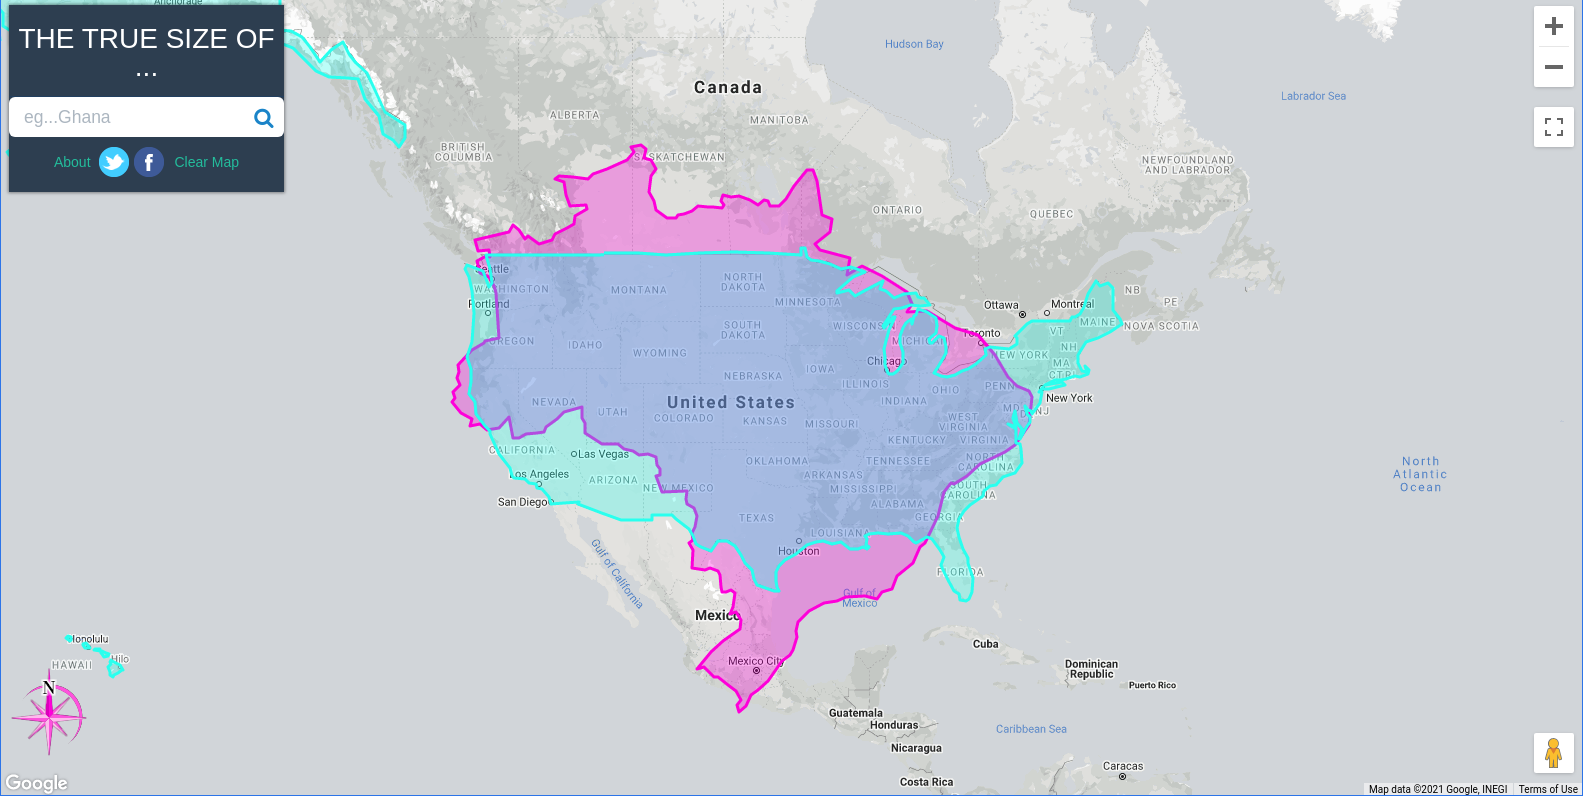
\includegraphics{_bookdown_files/_main_files/figure-html/media/modulo0/true-size-of.png}
\caption{True Size Of}
\end{figure}

\hypertarget{detalhando-os-conceitos}{%
\subsubsection{Detalhando os conceitos}\label{detalhando-os-conceitos}}

Então por que isso acontece? Como você aprenderá neste módulo, é difícil representar a forma tridimensional da Terra em uma folha de papel plana. Para fazer isso, os cartógrafos usam o que é chamado de \textbf{projeção cartográfica}, para projetar os pontos da superfície tridimensional da Terra em uma superfície plana. No entanto, ao fazer isso, eles introduzem alguma \textbf{distorção}. Essa distorção pode ser de forma, tamanho, direção e distâncias dos objetos representados no mapa. Todos os mapas têm pelo menos uma dessas distorções. Por causa dessa distorção, um mapa nunca pode mostrar toda a verdade sobre a Terra.

No mapa online que usamos, o mapa de fundo que não muda de tamanho (em cinza) é um exemplo de \textbf{dados raster}. Os dados raster são representações do mundo baseadas em pixels, semelhantes a como fotografias funcionam. Enquanto isso, a forma dos países que podemos mover são exemplos de \textbf{dados vetor, ou vetoriais}. Os dados vetoriais, ao contrário dos rasters, representam o mundo usando objetos discretos (no sentido matemático da palavra), como pontos, linhas e polígonos.

\hypertarget{conteuxfado-principal}{%
\subsection{Conteúdo principal}\label{conteuxfado-principal}}

\hypertarget{tuxedtulo-da-fase-1-mapas-e-coordenadas}{%
\subsubsection{Título da Fase 1: Mapas e Coordenadas}\label{tuxedtulo-da-fase-1-mapas-e-coordenadas}}

\hypertarget{conteuxfado-tutorial}{%
\paragraph{Conteúdo / Tutorial}\label{conteuxfado-tutorial}}

Quando as pessoas pensam na Terra atualmente, elas geralmente imaginam uma massa esférica azul, verde, branca e marrom flutuando no espaço. É por isso que tradicionalmente usamos globos para representar a Terra.

Figura 1. A Bola de Gude Azul ( https://commons.wikimedia.org/wiki/Earth\#/media/File:The\_Blue\_Marble.jpg)

Figura 2. Globo de l'Isle (1765) ( https://commons.wikimedia.org/wiki/Globe\#/media/File:3quarter\_globe.jpg)

No entanto, embora o globo seja capaz de capturar a maioria das características da Terra, ele possui duas desvantagens principais:

\begin{itemize}
\tightlist
\item
  Os globos são pesados e difíceis de transportar.
\item
  Os globos só podem ser usados em pequenas escalas (por exemplo, encontrar locais de países, as posições relativas de cidades, etc.). Eles são praticamente inúteis para atividades que exigem grandes escalas ou detalhes finos (por exemplo, navegação dentro de uma cidade).
\end{itemize}

É aqui que entram os mapas. Os mapas corrigem essas duas desvantagens dos globos, representando a Terra como uma superfície plana. Ao fazer isso, os mapas se tornam portáteis e adequados para uma infinidade de usos. Dito isso, os mapas também apresentam uma desvantagem própria. Através do processo de conversão de um objeto tridimensional (globo) em um bidimensional (mapa), distorções são geradas, de tal forma que é impossível para um mapa capturar perfeitamente as diferentes características da Terra (ou seja, formas, áreas e direções).

\hypertarget{projeuxe7uxf5es-cartogruxe1ficas}{%
\subparagraph{Projeções cartográficas}\label{projeuxe7uxf5es-cartogruxe1ficas}}

Uma projeção cartográfica é usada para achatar a superfície da Terra (ou de um globo qualquer) em um plano, a fim de criar um mapa. Este processo de transformação gera distorção.

\begin{figure}
\centering
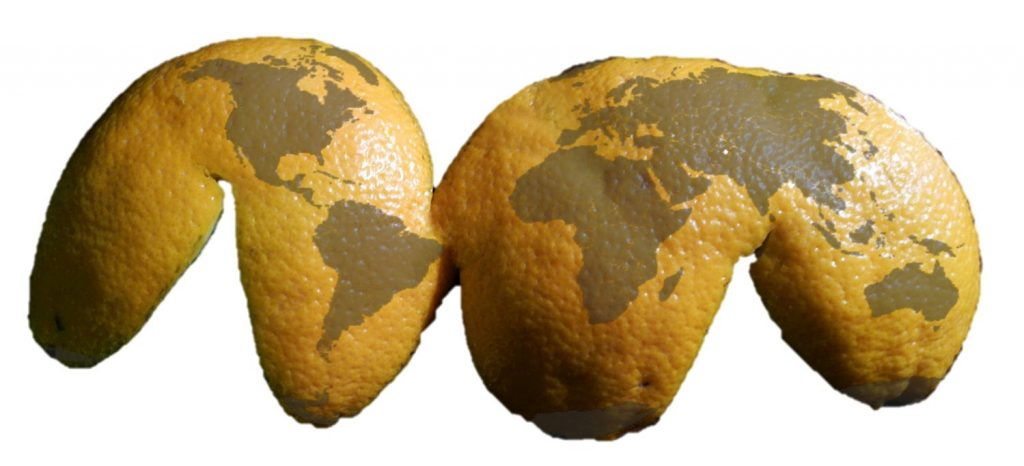
\includegraphics{_bookdown_files/_main_files/figure-html/media/modulo0/dalandan.png}
\caption{A terra como uma laranja}
\end{figure}

Pense na Terra como uma laranja. Se você descascá-la, poderá deixá-la plana, mas nunca poderá torná-la perfeitamente plana. Você sempre encontrará um dos seguintes problemas:

\begin{itemize}
\tightlist
\item
  \textbf{Alongamento} - o alongamento da casca (ou superfície) em uma ou mais direções
\item
  \textbf{Rasgos} - a divisão ou ruptura da casca (ou superfície)
\item
  \textbf{Compressão} - o encurtamento ou encolhimento da casca (ou superfície)
\end{itemize}

Por causa desses problemas, cada mapa contém distorção em uma ou mais das seguintes características:

\begin{itemize}
\tightlist
\item
  \textbf{Forma}
\item
  \textbf{Área}
\item
  \textbf{Distância}
\item
  \textbf{Direção}
\end{itemize}

As projeções cartográficas podem preservar (sem distorção) uma ou mais dessas características, mas nunca todas ao mesmo tempo. Outra opção é balancear e minimizar as distorções para todas as características ao mesmo tempo. Isso se deve à natureza das próprias características.

Características principais como \textbf{Forma} e \textbf{Área} são \textbf{mutuamente excludentes} e não podem ser preservadas simultaneamente. Enquanto isso, as características secundárias \textbf{Distância} e \textbf{Direção} \textbf{não têm como estar corretas em todos os lugares} do mapa.

Ao escolher qual projeção cartográfica usar, é importante que você considere o propósito do mapa. Por exemplo, se deseja realizar análises baseadas em área, é melhor usar uma projeção cartográfica que preserva a área.

Existem várias classificações de projeções cartográficas. A primeira é baseada nas \textbf{características que elas preservam}.

\begin{itemize}
\tightlist
\item
  Projeções de mapa \textbf{conforme} ou \textbf{ortomórficas} são aquelas que preservam a forma ou a conformidade angular. Estes são comumente usados para fins de navegação ou meteorológicos. As formas são preservadas, mas as áreas são distorcidas. Quanto maior a área, maior a distorção.
\item
  Projeções de mapa de \textbf{equivalente} ou \textbf{de igual área} são aquelas que preservam a proporção ou áreas relativas dos objetos no mapa. Nesse tipo de projeção cartográfica, quanto maior a área mapeada, mais precisa ela será.
\item
  As projeções cartográficas \textbf{equidistantes} preservam a distância das linhas que originam em um ou dois pontos no mapa ou têm escala adequada ao longo de uma ou mais linhas.
\item
  As projeções cartográficas \textbf{azimutais} preservam a direção a partir de um ou dois pontos no mapa. São úteis para mapear rotas de aeronaves e embarcações marítimas entre portos.
\end{itemize}

Uma única projeção cartográfica pode preservar mais de uma característica (por exemplo, uma projeção azimutal equidistante que preserva a direção e as distâncias a partir de um ou dois pontos no mapa), mas nem todas delas, como mostrado na tabela abaixo.

Conforme

Equivalente

Equidistante

Azimutal

Conforme

\begin{itemize}
\item
  Não

  Não

  Sim

  Equivalente

  Não

  \begin{itemize}
  \item
    Não

    Sim

    Equidistante

    Não

    Não

    \begin{itemize}
    \item
      Sim

      Azimutal

      Sim

      Sim

      Sim

      \begin{itemize}
      \tightlist
      \item
      \end{itemize}
    \end{itemize}
  \end{itemize}
\end{itemize}

Tabela: Ambas características podem ser preservadas por um mapa ao mesmo tempo?

Existe outra classificação de projeções cartográficas que não preserva nenhuma das características do mapa, mas tenta minimizar todas as distorções no mapa. Estes são chamados de projeções \textbf{Erro Mínimo (Minimum Error, ou Compromise)} (mapas que não preservam a forma nem a área são chamados de \textbf{Afiláticos}).

Uma maneira de visualizar a distorção é usando o que é chamado de \textbf{indicador de Tissot}. Este indicador caracteriza as distorções locais usando círculos e mostrando como esses círculos são transformados ao longo do mapa.

\begin{figure}
\centering
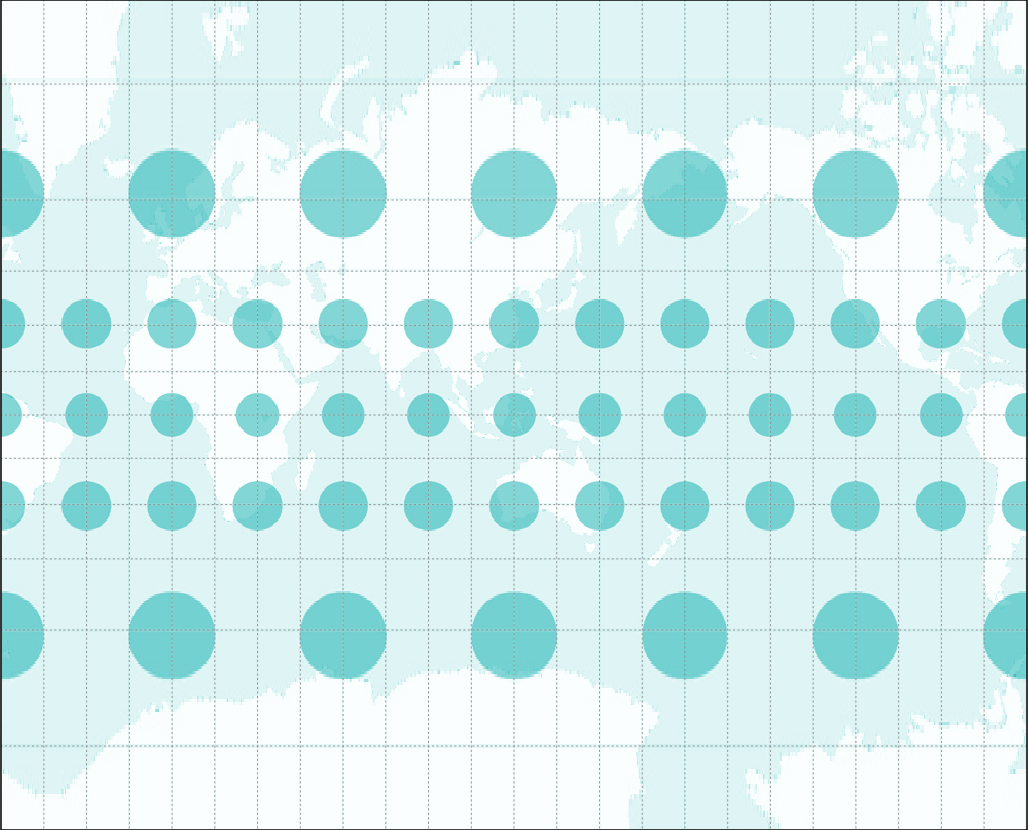
\includegraphics{_bookdown_files/_main_files/figure-html/media/modulo0/conformal.png}
\caption{Projeção conforme}
\end{figure}

Figura 3. Projeção conforme com seu índice de Tissot. Os círculos permanecem como círculos por todo o mapa, mas suas áreas aumentam a medida que os círculos se movem do equador em direção aos pólos.

\begin{figure}
\centering
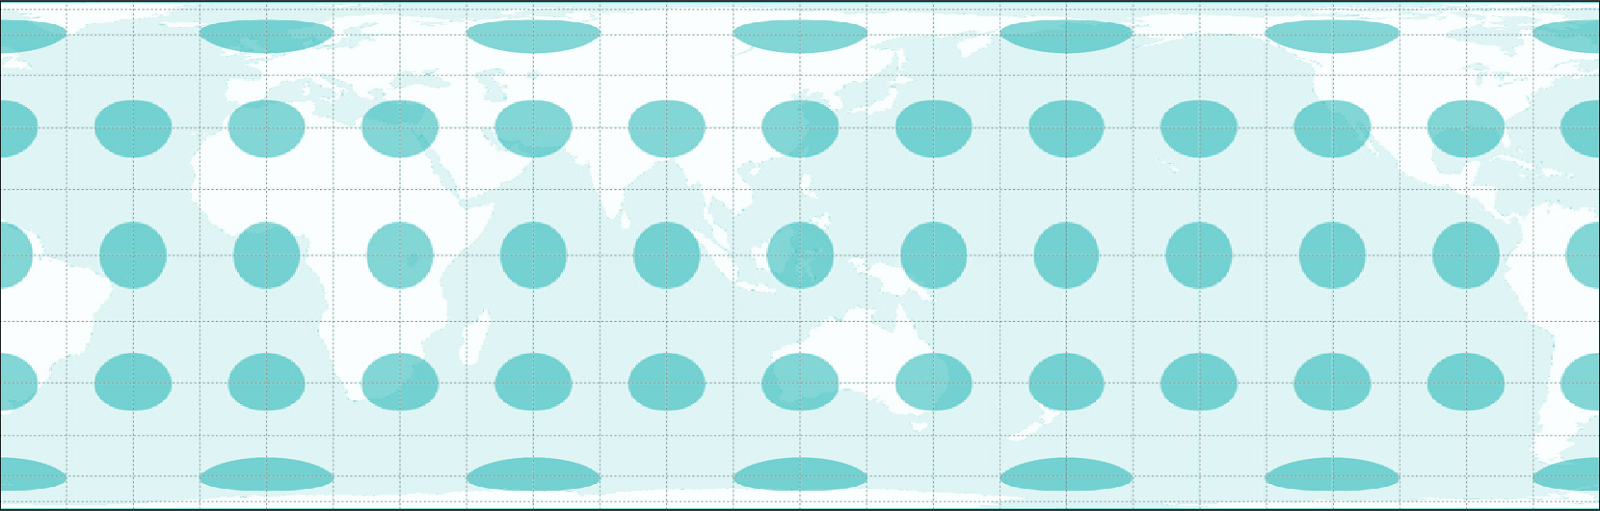
\includegraphics{_bookdown_files/_main_files/figure-html/media/modulo0/authalic.png}
\caption{Projeção equivalente}
\end{figure}

Figura 4. Projeção equivalente com seu índice de Tissot. Os círculos tornam-se elipses, mas suas áreas permanecem as mesmas.

\begin{figure}
\centering
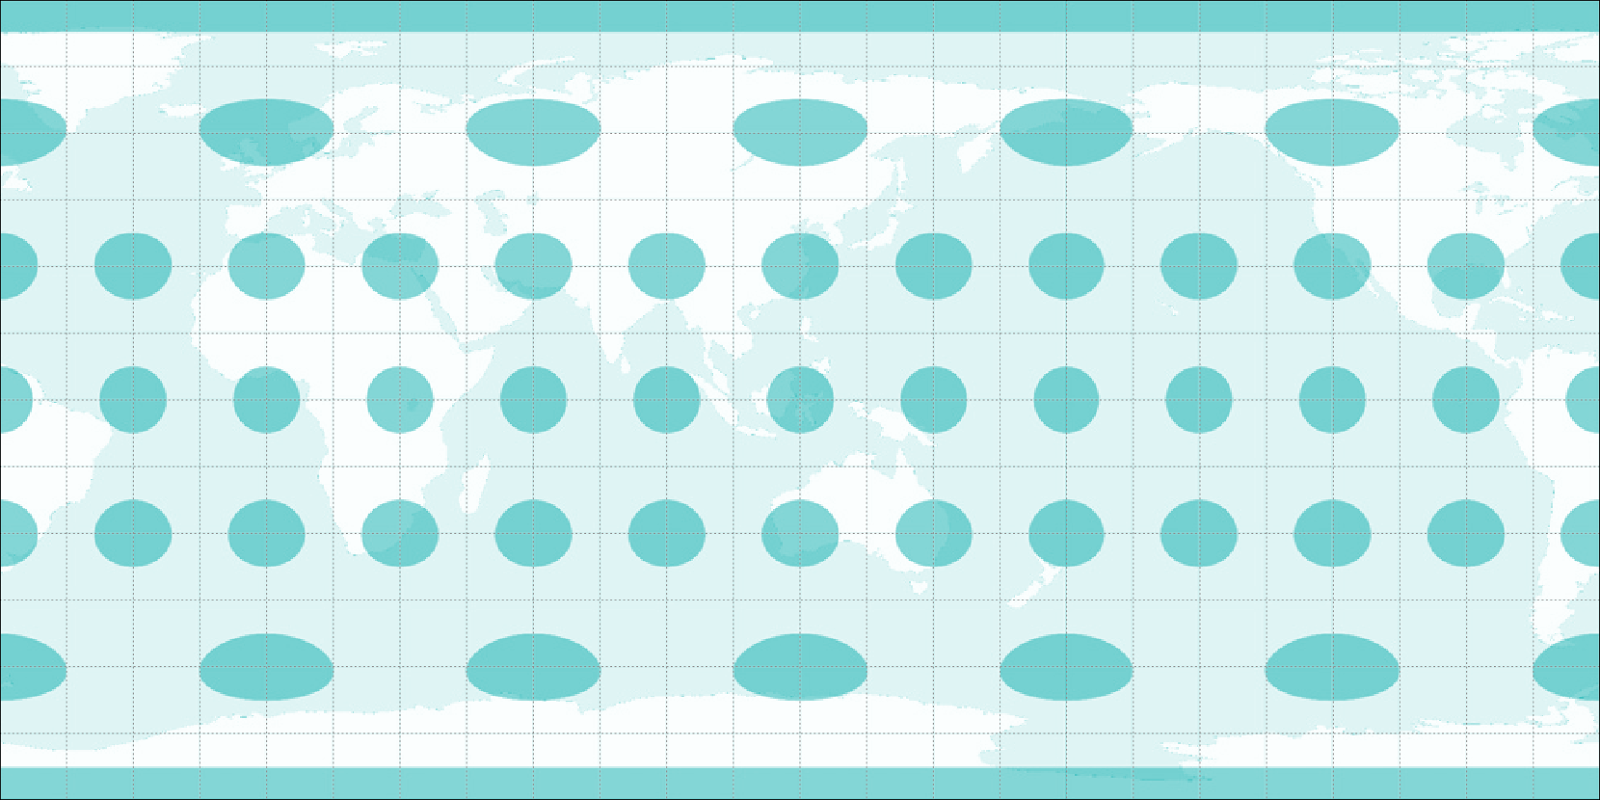
\includegraphics{_bookdown_files/_main_files/figure-html/media/modulo0/equidistant.png}
\caption{Projeção equidistante}
\end{figure}

Figura 5. Projeção equidistante com seu índice de Tissot. Observe que as alturas dos círculos são iguais, o que significa que a escala / distâncias ao longo dos meridianos são preservadas.

\begin{figure}
\centering

\includegraphics{_bookdown_files/_main_files/figure-html/media/modulo0/az-equidistant.png}
\caption{Projeção azimutal equidistante}
\end{figure}

Figura 6. Projeção azimutal equidistante com seu índice de Tissot. Observe que os círculos estão todos apontando para o centro do mapa e as alturas dos círculos são todas iguais.

Outra maneira de classificar as projeções do mapa é pela \textbf{superfície desenvolvível (``developable surface'')} usada para criar o mapa. Uma superfície é desenvolvível se ela puder ser planificada sem introduzir distorções. As superfícies mais comumente usadas são: Cilindros (Figura 7), Cones (Figura 8) e Planos (Figura 9).

\begin{figure}
\centering
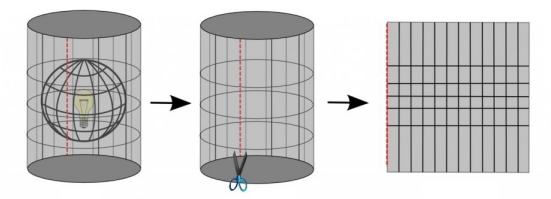
\includegraphics{_bookdown_files/_main_files/figure-html/media/modulo0/cylinder.png}
\caption{Cilindro como uma superfície desenvolvível}
\end{figure}

Figura 7. As projeções cilíndricas têm meridianos (longitude) e paralelos (latitude) encontrando-se em ângulos retos com as distâncias entre os meridianos sendo iguais.

\begin{figure}
\centering
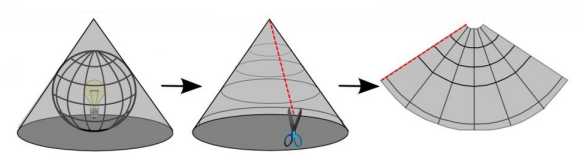
\includegraphics{_bookdown_files/_main_files/figure-html/media/modulo0/cone.png}
\caption{Cone como superfície desenvolvível}
\end{figure}

Figura 8. As projeções cônicas têm meridianos retos indo para um ponto nos pólos. Os paralelos são arcos.

\begin{figure}
\centering
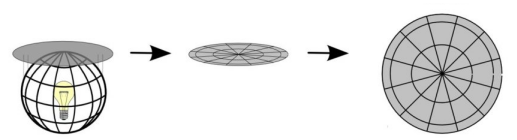
\includegraphics{_bookdown_files/_main_files/figure-html/media/modulo0/plane.png}
\caption{Plano como superfície desenvolvível}
\end{figure}

Figura 9. As projeções planas (comumente usadas em projeções azimutais) têm meridianos retos semelhantes às projeções cônicas, mas seus paralelos são círculos em vez de arcos.

Existem inúmeras outras superfícies desenvolvíveis que podem ser usadas para transformar um globo em um mapa. Eles podem ser uma variação das superfícies comuns, como no caso de projeções pseudo-cilíndricas e pseudo-cônicas ou podem ser superfícies únicas e diferentes, como no mapa Dymaxion, que usa um icosaedro (poliedro com 20 faces), ou a Projeção de Cahill-Keyes que usa um octaedro (poliedro com 8 faces).

A projeção de um mapa também pode ser classificada de acordo com seu \textbf{aspecto} (Figura 10) ou o modo como a superfície desenvolvível está posicionada no globo: Normal, Transversal ou Oblíqua.

\begin{figure}
\centering
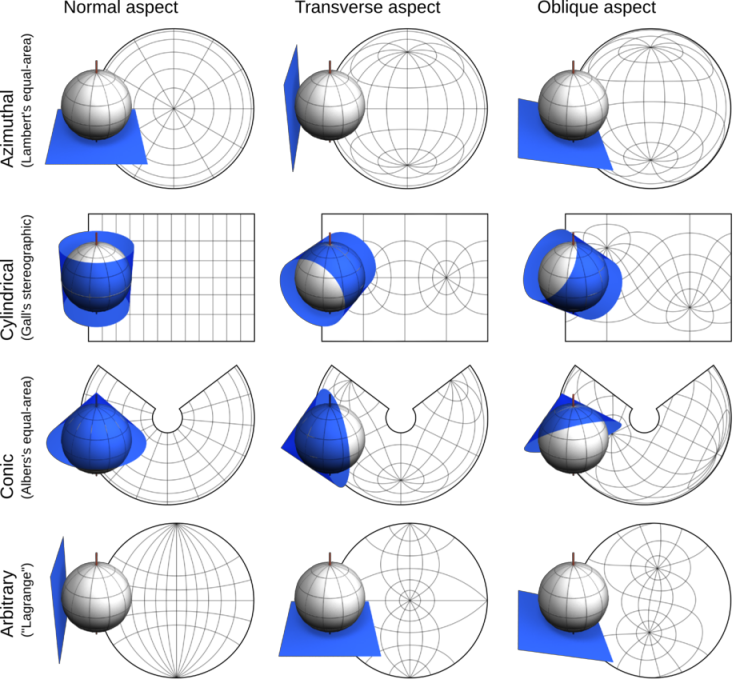
\includegraphics{_bookdown_files/_main_files/figure-html/media/modulo0/aspects.png}
\caption{Aspectos de uma projeção cartográfica}
\end{figure}

Figura 10. Aspectos de uma projeção cartográfica

\hypertarget{sistemas-de-referuxeancia-de-coordenadas}{%
\subparagraph{Sistemas de referência de coordenadas}\label{sistemas-de-referuxeancia-de-coordenadas}}

Um \textbf{Sistema de Referência de Coordenadas (SRC, ou CRS na sigla em inglês)} é usado para especificar a localização de um objeto na superfície da Terra por meio do uso de coordenadas. SRCs podem ser classificados em dois:

\begin{itemize}
\tightlist
\item
  \textbf{Sistemas de referência de coordenadas geográficas} usam graus de latitude e longitude como coordenadas para se referir à posição.
\item
  \textbf{Sistemas de referência de coordenadas projetadas} usam unidades lineares (por exemplo, metros, pés, quilômetros) de leste e norte como coordenadas.
\end{itemize}

O conhecimento dos sistemas de referência de coordenadas é importante porque mesmo que dois mapas (ou camadas) mostrem o mesmo local, as coordenadas das localizações nesses mapas serão diferentes se os SRC que eles usam forem diferentes.

\textbf{Veja este exemplo:} Mapa A e Mapa B mostram a mesma área e extensão. Eles são basicamente o mesmo mapa. A única diferença é o sistema de referência de coordenadas que eles usam. O Mapa A usa SRC X e o Mapa B usa SRC Y. Digamos que obtivemos a coordenada do Ponto 1, que é (10, 10), do Mapa A. Se olharmos para a coordenada (10,10) no Mapa B, é possível que o Ponto 1 não esteja lá, pois o Mapa B usa um SRC diferente. Ou, se você sobrepor os mapas um ao outro usando uma referência comum, os objetos dos dois mapas não coincidirão. Este conhecimento de sistemas de referência de coordenadas é importante para qualquer tipo de GIS.

As versões do QGIS anteriores à versão 3 tinham a opção de ativar o que é chamado de ``OTF'' ou ``Transformação On-The-Fly (em `tempo real')''. Isso permitia que camadas com diferentes SRC fossem projetadas na tela do mapa como se estivessem no mesmo SRC. Com o QGIS 3 em diante, esta opção é ativada automaticamente como comportamento padrão do QGIS. QGIS também executa esta ação automaticamente para tarefas de processamento. Isso é muito importante porque se as camadas não estiverem no mesmo SRC, os resultados das consultas espaciais e do processamento como junções espaciais, clipes, etc. podem ser comprometidos.

Você pode notar que alguns Sistemas de Referência de Coordenadas são referidos por seu Código EPSG. Este código se refere ao código do SRC no conjunto de dados de parâmetros geodésicos EPSG, que é um registro de dados geodésicos, sistemas de referência espacial, elipsóides terrestres, transformações de coordenadas e unidades de medida relacionadas. A maioria dos GIS, incluindo QGIS, referem-se ao código EPSG para identificar sistemas de referência de coordenadas, projeções e realizar transformações entre esses sistemas.

Alguns códigos EPSG comuns incluem:

\begin{itemize}
\tightlist
\item
  \textbf{EPSG: 4326} - WGS 84, sistema de coordenadas de latitude / longitude baseado no Sistema de Posicionamento Global (GPS) entre outros.
\item
  \textbf{EPSG: 3857} - Projeção Web Mercator usada para exibição por muitas ferramentas de mapeamento baseadas na web, como OpenStreetMap e Google Maps
\item
  \textbf{EPSG: 31973 a EPSG: 31974 e EPSG: 31978 a EPSG: 31985} - Universal Transverse Mercator (UTM) Zonas 19N a 20N, e 18S a 25S. Zonas UTM usadas no Brasil
\item
  \textbf{EPSG: 4674} - Sistema de Referência SIRGAS 2000, utilizado nas Américas a partir do ano 2000
\end{itemize}

\hypertarget{quiz}{%
\paragraph{Quiz}\label{quiz}}

\begin{enumerate}
\def\labelenumi{\arabic{enumi}.}
\tightlist
\item
  Que tipo de projeção é melhor para os seguintes casos?

  \begin{enumerate}
  \def\labelenumii{\arabic{enumii}.}
  \tightlist
  \item
    um mapa de uso geral que precisa ter uma aparência agradável
  \item
    um mapa mostrando uma análise de área por unidade entre diferentes locais
  \item
    um mapa que mostra uma comparação de uma zona de 10 km de raio de diferentes locais
  \end{enumerate}
\item
  Que tipo de sistema de referência de coordenadas (geográfico ou projetado) é melhor utilizado para os seguintes casos?

  \begin{enumerate}
  \def\labelenumii{\arabic{enumii}.}
  \setcounter{enumii}{3}
  \tightlist
  \item
    mostrar a localização de pontos usando GPS
  \item
    calcular a distância entre dois pontos
  \end{enumerate}
\item
  Verdadeiro ou falso - É possível preservar as seguintes características do mapa juntas em um único mapa:

  \begin{enumerate}
  \def\labelenumii{\arabic{enumii}.}
  \setcounter{enumii}{5}
  \tightlist
  \item
    Área e forma
  \item
    Distância e direção
  \end{enumerate}
\end{enumerate}

\hypertarget{tuxedtulo-da-fase-2-tipos-de-dados-espaciais}{%
\subsubsection{Título da fase 2: Tipos de dados espaciais}\label{tuxedtulo-da-fase-2-tipos-de-dados-espaciais}}

\hypertarget{conteuxfado-tutorial-1}{%
\paragraph{Conteúdo / Tutorial}\label{conteuxfado-tutorial-1}}

Em sua essência, um Sistema de Informação Geográfica (SIG) deve ser capaz de modelar objetos, informações e fenômenos do mundo real, como limites de lotes, rios, estradas, temperatura, etc. Ele faz isso por meio de modelos de dados espaciais.

Os modelos de dados espaciais são compostos de dois componentes principais que, quando combinados, modelam a realidade. Esses componentes são:

\begin{itemize}
\tightlist
\item
  \textbf{Feições espaciais (ou geometria)}
\item
  \textbf{Atributos}
\end{itemize}

\begin{figure}
\centering
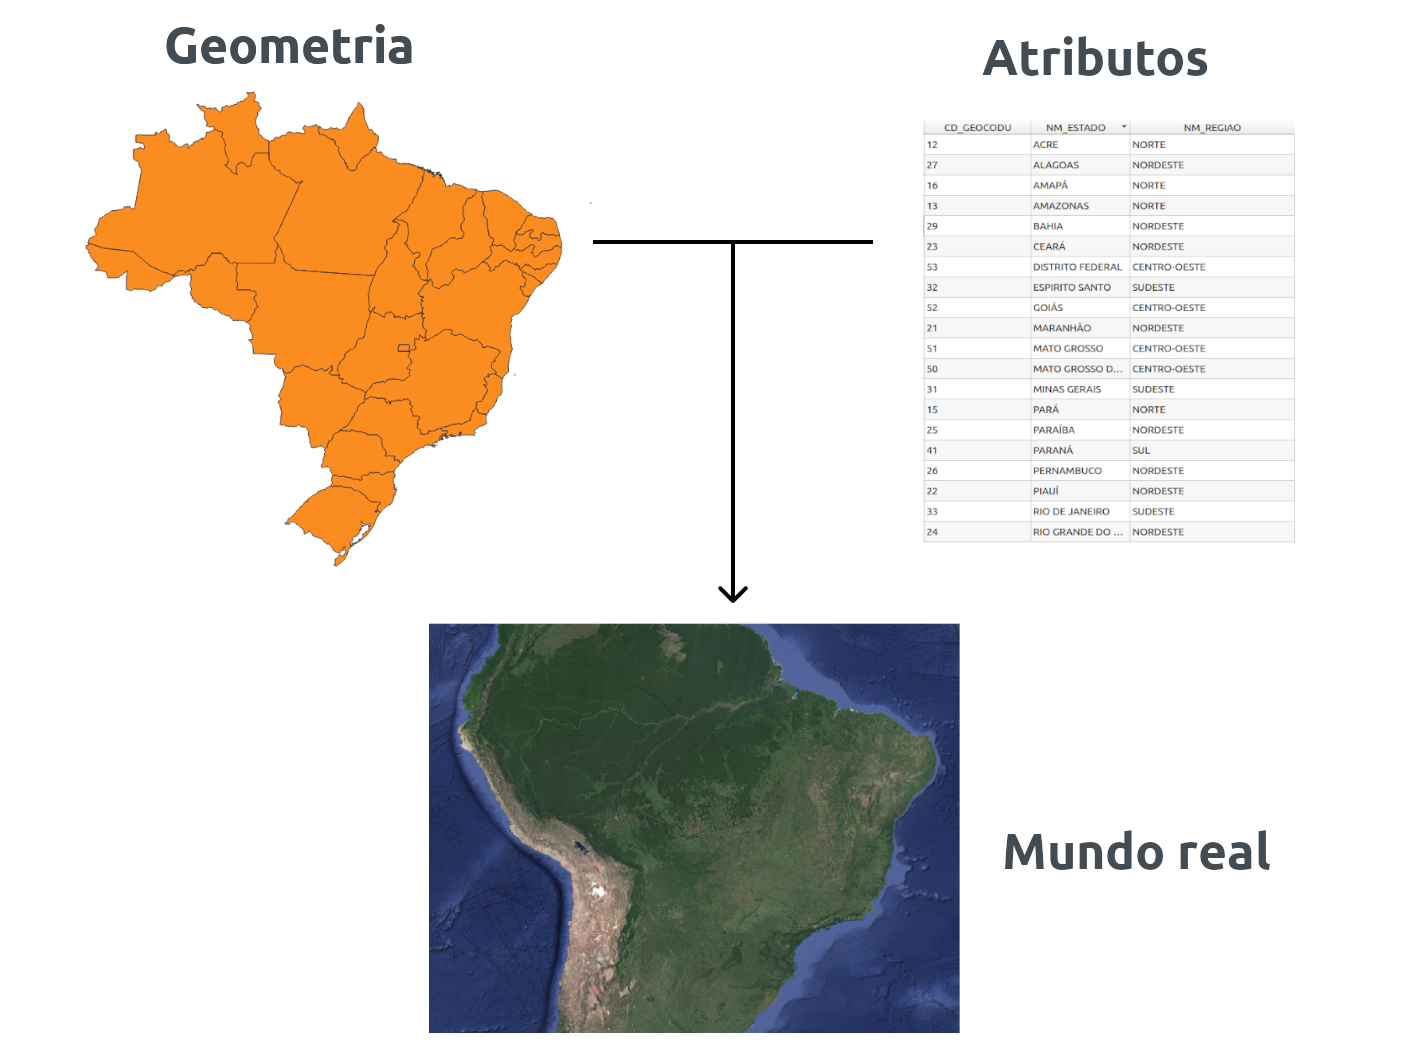
\includegraphics{_bookdown_files/_main_files/figure-html/media/modulo0/spatial-model.png}
\caption{Modelo de dados espaciais}
\end{figure}

Existem dois modelos principais de dados espaciais: \textbf{raster} e \textbf{vetorial}. Embora qualquer objeto do mundo real possa ser representado por qualquer um dos dois modelos de dados, um deles é geralmente melhor para representar certos objetos do mundo real do que o outro.

\hypertarget{dados-raster}{%
\subparagraph{Dados raster}\label{dados-raster}}

Os dados raster são mais utilizados para representar fenômenos contínuos, como elevação ou temperatura.

Um raster é uma representação de objetos do mundo real composta de linhas e colunas de células ou pixels, no qual cada célula ou pixel representa uma área geográfica (pense em uma fotografia ou imagem). O valor da célula representa o valor de um atributo na referida área geográfica. O tamanho da área depende da resolução espacial do raster.

Rasters são bastante úteis para modelagem de adequação de locais (suitability modelling), pois você pode combinar rasters por meio de operações matemáticas (álgebra de raster).

\begin{figure}
\centering
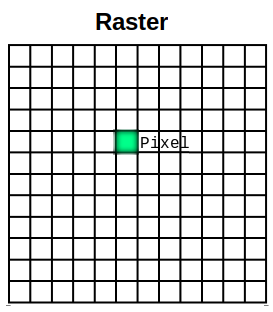
\includegraphics{_bookdown_files/_main_files/figure-html/media/modulo0/raster.png}
\caption{Modelo de dados raster}
\end{figure}

Figura 12. Um raster consiste em pixels de tamanhos iguais em linhas e colunas.

Um pixel raster pode conter apenas um valor de cada vez. Assim, um raster pode modelar apenas um objeto ou fenômeno por vez.

\hypertarget{dados-vetoriais}{%
\subparagraph{Dados vetoriais}\label{dados-vetoriais}}

Os dados vetoriais são mais utilizados para representar objetos discretos.

Os dados vetoriais possuem três formas: ponto, linha e polígono. São mais preciso que rasters porque pontos, linhas e polígonos são modelados usando coordenadas bem definidas, tornando-os melhores na representação de objetos discretos do que rasters.

Os vetores são comumente usados quando necessitamos precisão com comprimentos, áreas e distâncias. Eles também são úteis ao realizar análises de rede (por exemplo, encontrar o caminho mais curto um ponto a outro em uma rede de vias).

\begin{figure}
\centering
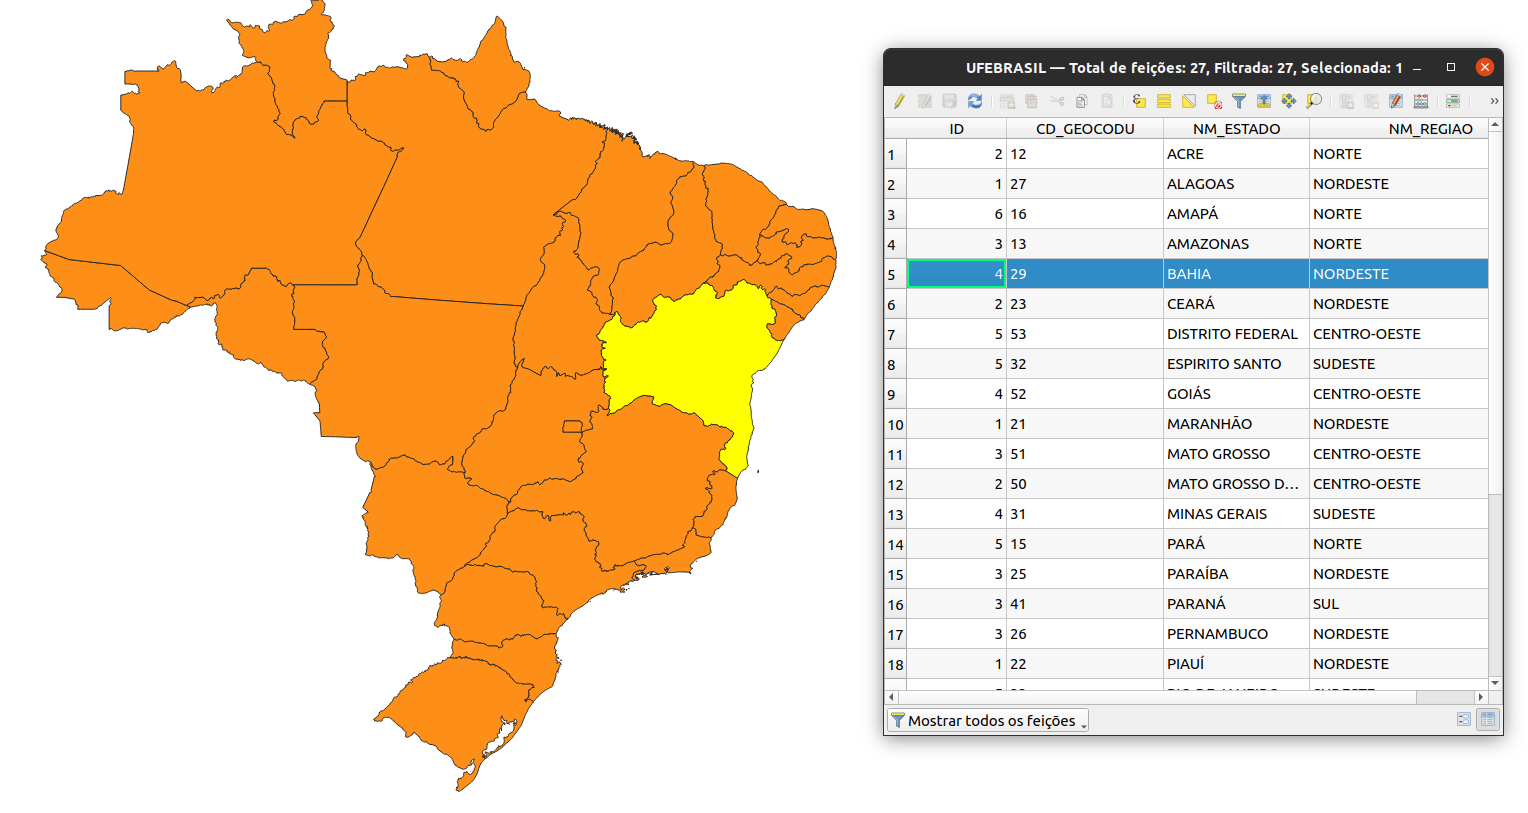
\includegraphics{_bookdown_files/_main_files/figure-html/media/modulo0/vector.png}
\caption{Modelo de dados vetoriais}
\end{figure}

Figura 13. Um vetor consiste em feições com seus atributos correspondentes.

Comparado aos pixels raster, uma feição vetorial pode conter mais de um valor por vez. Esses valores são armazenados como colunas na tabela de atributos. Cada feição é armazenada como uma linha.

\hypertarget{quiz-1}{%
\paragraph{Quiz}\label{quiz-1}}

\begin{enumerate}
\def\labelenumi{\arabic{enumi}.}
\tightlist
\item
  Qual tipo de dado pode representar melhor os seguintes objetos / fenômenos:

  \begin{enumerate}
  \def\labelenumii{\arabic{enumii}.}
  \tightlist
  \item
    estradas
  \item
    casas
  \item
    densidade populacional
  \item
    perigo de inundação
  \end{enumerate}
\end{enumerate}

\hypertarget{tuxedtulo-da-fase-3-sistema-de-informauxe7uxe3o-geogruxe1fica-sig}{%
\subsubsection{Título da Fase 3: Sistema de Informação Geográfica (SIG)}\label{tuxedtulo-da-fase-3-sistema-de-informauxe7uxe3o-geogruxe1fica-sig}}

\hypertarget{conteuxfado-tutorial-2}{%
\paragraph{Conteúdo / Tutorial}\label{conteuxfado-tutorial-2}}

As informações geográficas e de localização tornaram-se onipresentes no século 21 em todos os níveis de granularidade. Temos satélites, aeronaves e até drones comerciais que são capazes de capturar grandes quantidades de dados brutos em grandes áreas por longos períodos de tempo. Existem também sensores que coletam e reúnem informações de localização, como o GPS e outros aplicativos em nossos telefones e dispositivos.

Com todos esses dados à nossa disposição, é fundamental saber gerenciá-los, analisá-los e apresentá-los. É aqui que entram os Sistemas de Informação Geográfica, ou mais comumente conhecidos como SIG, ou GIS.

SIG é uma ferramenta / framework / sistema que nos permite trabalhar com informação geográfica (ou espacial) e sua correspondente informação de atributo (não espacial). Em particular, um GIS deve ser capaz de:

\begin{itemize}
\tightlist
\item
  \textbf{Coletar}, \textbf{armazenar}, \textbf{editar}, \textbf{manipular}, ou em termos mais gerais, \textbf{gerenciar} dados espaciais.
\item
  \textbf{Analizar} os dados usando seu componente espacial (onde os dados estão) ou atributo (o valor dos dados).
\item
  \textbf{Apresentar} os dados e análises como informações significativas por meio de mapas, gráficos, plotagens e outras visualizações.
\end{itemize}

\emph{SIG não é apenas mapeamento}. Embora a elaboração de mapas seja um dos aspectos mais importantes e comumente conhecidos do SIG, ela ainda é apenas uma parte de seus muitos recursos. Podemos ver a estrutura SIG moderna como sendo composta por:

\begin{itemize}
\tightlist
\item
  \textbf{Dados} - referem-se às informações utilizadas pelo SIG que podem ou não conter informações de localização (por exemplo, nomes de lojas, localizações de lojas).
\item
  \textbf{Tecnologia} - inclui os componentes de hardware e software de um SIG - as máquinas, instrumentos e computadores com os aplicativos de software usados para fazer o trabalho geoespacial.
\item
  \textbf{Métodos e análises} - referem-se à ciência e matemática em SIG, que permitem realizar consultas e cálculos espaciais e não espaciais (de atributos).
\item
  \textbf{Visualização} - embora semelhante aos métodos e análises, a visualização pode ser considerada como um componente separado, pois se refere especificamente aos meios pelos quais um SIG representa os dados graficamente. Isso inclui não apenas mapas, embora seja o caso mais comum, mas também tabelas, gráficos, etc.
\item
  \textbf{Pessoas} - são as pessoas e / ou grupos de pessoas que estão envolvidas no uso, desenvolvimento, ensino e manutenção de SIG.
\end{itemize}

Todas as partes da estrutura SIG moderna - dos dados às pessoas - são essenciais para garantir seu sucesso.

\hypertarget{perguntas-do-questionuxe1rio}{%
\paragraph{Perguntas do questionário}\label{perguntas-do-questionuxe1rio}}

\begin{enumerate}
\def\labelenumi{\arabic{enumi}.}
\tightlist
\item
  Verdadeiro ou falso:

  \begin{enumerate}
  \def\labelenumii{\arabic{enumii}.}
  \tightlist
  \item
    Um SIG só pode ser usado com dados geoespaciais.
  \item
    Um mapa é sempre o resultado ao se usar um SIG.
  \item
    Aprender SIG é difícil e caro.
  \end{enumerate}
\end{enumerate}

\hypertarget{tuxedtulo-da-fase-4-adicional-software-livre-e-de-cuxf3digo-aberto-para-uso-geoespacial-foss4g}{%
\subsubsection{Título da Fase 4 (adicional): Software Livre e de Código Aberto para uso Geoespacial (FOSS4G)}\label{tuxedtulo-da-fase-4-adicional-software-livre-e-de-cuxf3digo-aberto-para-uso-geoespacial-foss4g}}

\hypertarget{conteuxfado-tutorial-3}{%
\paragraph{Conteúdo / Tutorial}\label{conteuxfado-tutorial-3}}

QGIS é apenas um exemplo de software livre e de código aberto para uso geoespacial (FOSS4G). Outros exemplos de FOSS4G são GRASS, PostGIS, GeoServer, GeoNode, etc. Esses aplicativos FOSS4G são ótimas ferramentas para trabalhar não só porque são confiáveis, mas também porque, sendo gratuitos e de código aberto, têm uma barreira de entrada menor e são altamente personalizáveis para qualquer necessidade. Você pode encontrar uma variedade de softwares geoespaciais gratuitos e de código aberto para cada necessidade e para cada parte do ``stack'' geoespacial.

\begin{figure}
\centering
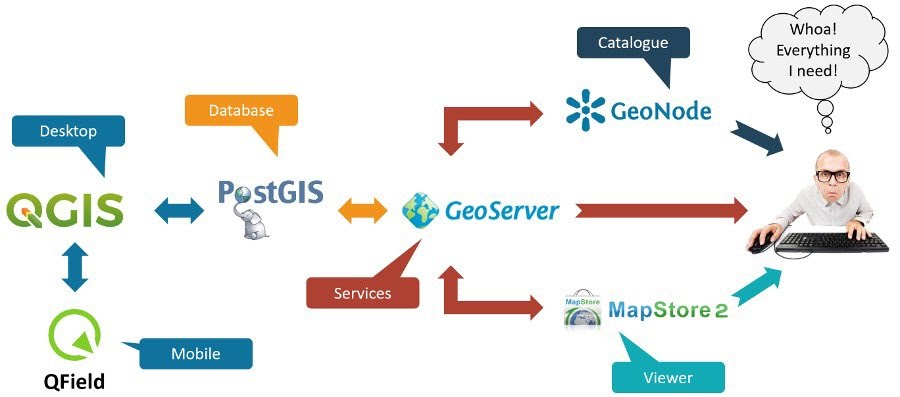
\includegraphics{_bookdown_files/_main_files/figure-html/media/modulo0/foss4g-stack.jpeg}
\caption{Stack de aplicativos de software livre e de código aberto para geoespaciais (FOSS4G)}
\end{figure}

Figura 14. Uma amostra de stack geoespacial de código aberto (ou FOSS4G) (de Simon Nitz (\url{https://twitter.com/si_nitz?lang=en}))

\hypertarget{software-gruxe1tis}{%
\subparagraph{Software grátis}\label{software-gruxe1tis}}

\textbf{Livre como em liberdade e não apenas grátis.}

Software livre é o software que adere às Quatro Liberdades Essenciais do Software Livre, que são:

\begin{enumerate}
\def\labelenumi{\arabic{enumi}.}
\tightlist
\item
  A liberdade de executar o programa como desejar, para qualquer propósito (liberdade 0).
\item
  A liberdade de estudar como o programa funciona e alterá-lo para que ele faça o que você deseja (liberdade 1). O acesso ao código-fonte é uma pré-condição para isso.
\item
  A liberdade de redistribuir cópias para que você possa ajudar outras pessoas (liberdade 2).
\item
  A liberdade de distribuir cópias de suas versões modificadas para outros (liberdade 3). Ao fazer isso, você pode dar a toda a comunidade a chance de se beneficiar com suas mudanças. O acesso ao código-fonte é uma pré-condição para isso.
\end{enumerate}

\hypertarget{cuxf3digo-aberto}{%
\subparagraph{Código aberto}\label{cuxf3digo-aberto}}

Softwares de código aberto são aqueles que possuem licenças que permitem uso sem precisar pagar royalties e que permitem a reutilização do software, juntamente com acesso livre ao código-fonte. Por convenção, essas licenças de código aberto são aquelas que estão em conformidade com a definição de código aberto prevista pela Open Source Initiative. O código-fonte aberto não só garante acesso gratuito ao software e código-fonte, mas também a capacidade de redistribuir o software sem custos adicionais.

Por causa da natureza aberta do software de código aberto, ele também é um ótimo modelo de desenvolvimento de software, no qual todos são livres para atualizar, melhorar, modificar e compartilhar suas modificações com a comunidade.

\hypertarget{osgeo}{%
\subparagraph{OSGeo}\label{osgeo}}

Existem muitos softwares geoespaciais de código aberto e, às vezes, a parte mais difícil é saber onde e como começar a trabalhar com esses softwares. Felizmente, a Open Source Geospatial Foundation (OSGeo) (\url{https://www.osgeo.org/}) existe para ajudar a promover a adoção global de tecnologia geoespacial aberta e apoiar o desenvolvimento dessas tecnologias.

\hypertarget{perguntas-do-questionuxe1rio-1}{%
\paragraph{Perguntas do questionário}\label{perguntas-do-questionuxe1rio-1}}

N/D

\hypertarget{se-vocuxea-quiser-ir-mais-longe}{%
\subsubsection{Se você quiser ir mais longe}\label{se-vocuxea-quiser-ir-mais-longe}}

Se você quiser testar usar aplicativos FOSS4G facilmente, experimente o OSGeoLive (\url{https://live.osgeo.org/en/index.html}) que é uma distribuição Linux (sistema operacional) que vem pré-instalado com QGIS, GRASS e outros aplicativos FOSS4G.

\hypertarget{para-praticar-suas-novas-habilidades-tente}{%
\subsubsection{Para praticar suas novas habilidades, tente\ldots{}}\label{para-praticar-suas-novas-habilidades-tente}}

N/D

\hypertarget{dicas}{%
\subsubsection{Dicas}\label{dicas}}

N/D

\hypertarget{introduuxe7uxe3o-ao-qgis}{%
\chapter{Introdução ao QGIS}\label{introduuxe7uxe3o-ao-qgis}}

\textbf{Autor}: Ben Hur

\hypertarget{introduuxe7uxe3o-pedaguxf3gica-1}{%
\section{Introdução Pedagógica}\label{introduuxe7uxe3o-pedaguxf3gica-1}}

Este módulo serve como uma introdução ao QGIS. No final deste módulo, os alunos devem estar familiarizados com:

\begin{itemize}
\tightlist
\item
  O que é o QGIS
\item
  Interface do QGIS
\item
  Configurações do QGIS
\item
  Complementos do QGIS
\end{itemize}

Eles também devem aprender:

\begin{itemize}
\tightlist
\item
  Como instalar e abrir o QGIS
\item
  As diferentes partes e recursos da interface do QGIS
\item
  Como editar o layout e o tema da interface
\item
  As diferentes configurações do QGIS, como alterá-las e como elas afetam o QGIS
\item
  O que são perfis de usuário e como usá-los
\item
  O que são complementos e como instalá-los
\end{itemize}

O módulo também irá discutir algumas nuances do QGIS e o que o torna único ou diferente de outros softwares GIS, como formatos de arquivo QGIS.

\hypertarget{ferramentas-e-recursos-necessuxe1rios-1}{%
\section{Ferramentas e recursos necessários}\label{ferramentas-e-recursos-necessuxe1rios-1}}

As ferramentas e recursos necessários para este módulo são:

\begin{itemize}
\tightlist
\item
  Computador
\item
  Conexão de internet
\item
  QGIS 3.16 instalado no computador (\url{https://qgis.org/en/site/forusers/download.html})
\end{itemize}

\hypertarget{pruxe9-requisitos-1}{%
\section{Pré-requisitos}\label{pruxe9-requisitos-1}}

\begin{itemize}
\tightlist
\item
  Conhecimento básico de informática
\end{itemize}

\hypertarget{recursos-adicionais-1}{%
\section{Recursos adicionais}\label{recursos-adicionais-1}}

\begin{itemize}
\tightlist
\item
  Manual do usuário QGIS - \url{https://docs.qgis.org/3.16/en/docs/user_manual/}
\item
  Manual de treinamento QGIS - \url{https://docs.qgis.org/3.16/en/docs/training_manual/index.html}
\end{itemize}

\hypertarget{introduuxe7uxe3o-temuxe1tica-1}{%
\section{Introdução temática}\label{introduuxe7uxe3o-temuxe1tica-1}}

O mapa abaixo (\url{https://flic.kr/p/2jFfGJP}), de Andrés Felipe Lancheros Sánchez, mostra partes da cidade de Bogotá na Colômbia feitas no estilo da pintura ``Noite estrelada'' de Vincent van Gogh.

\begin{figure}
\centering
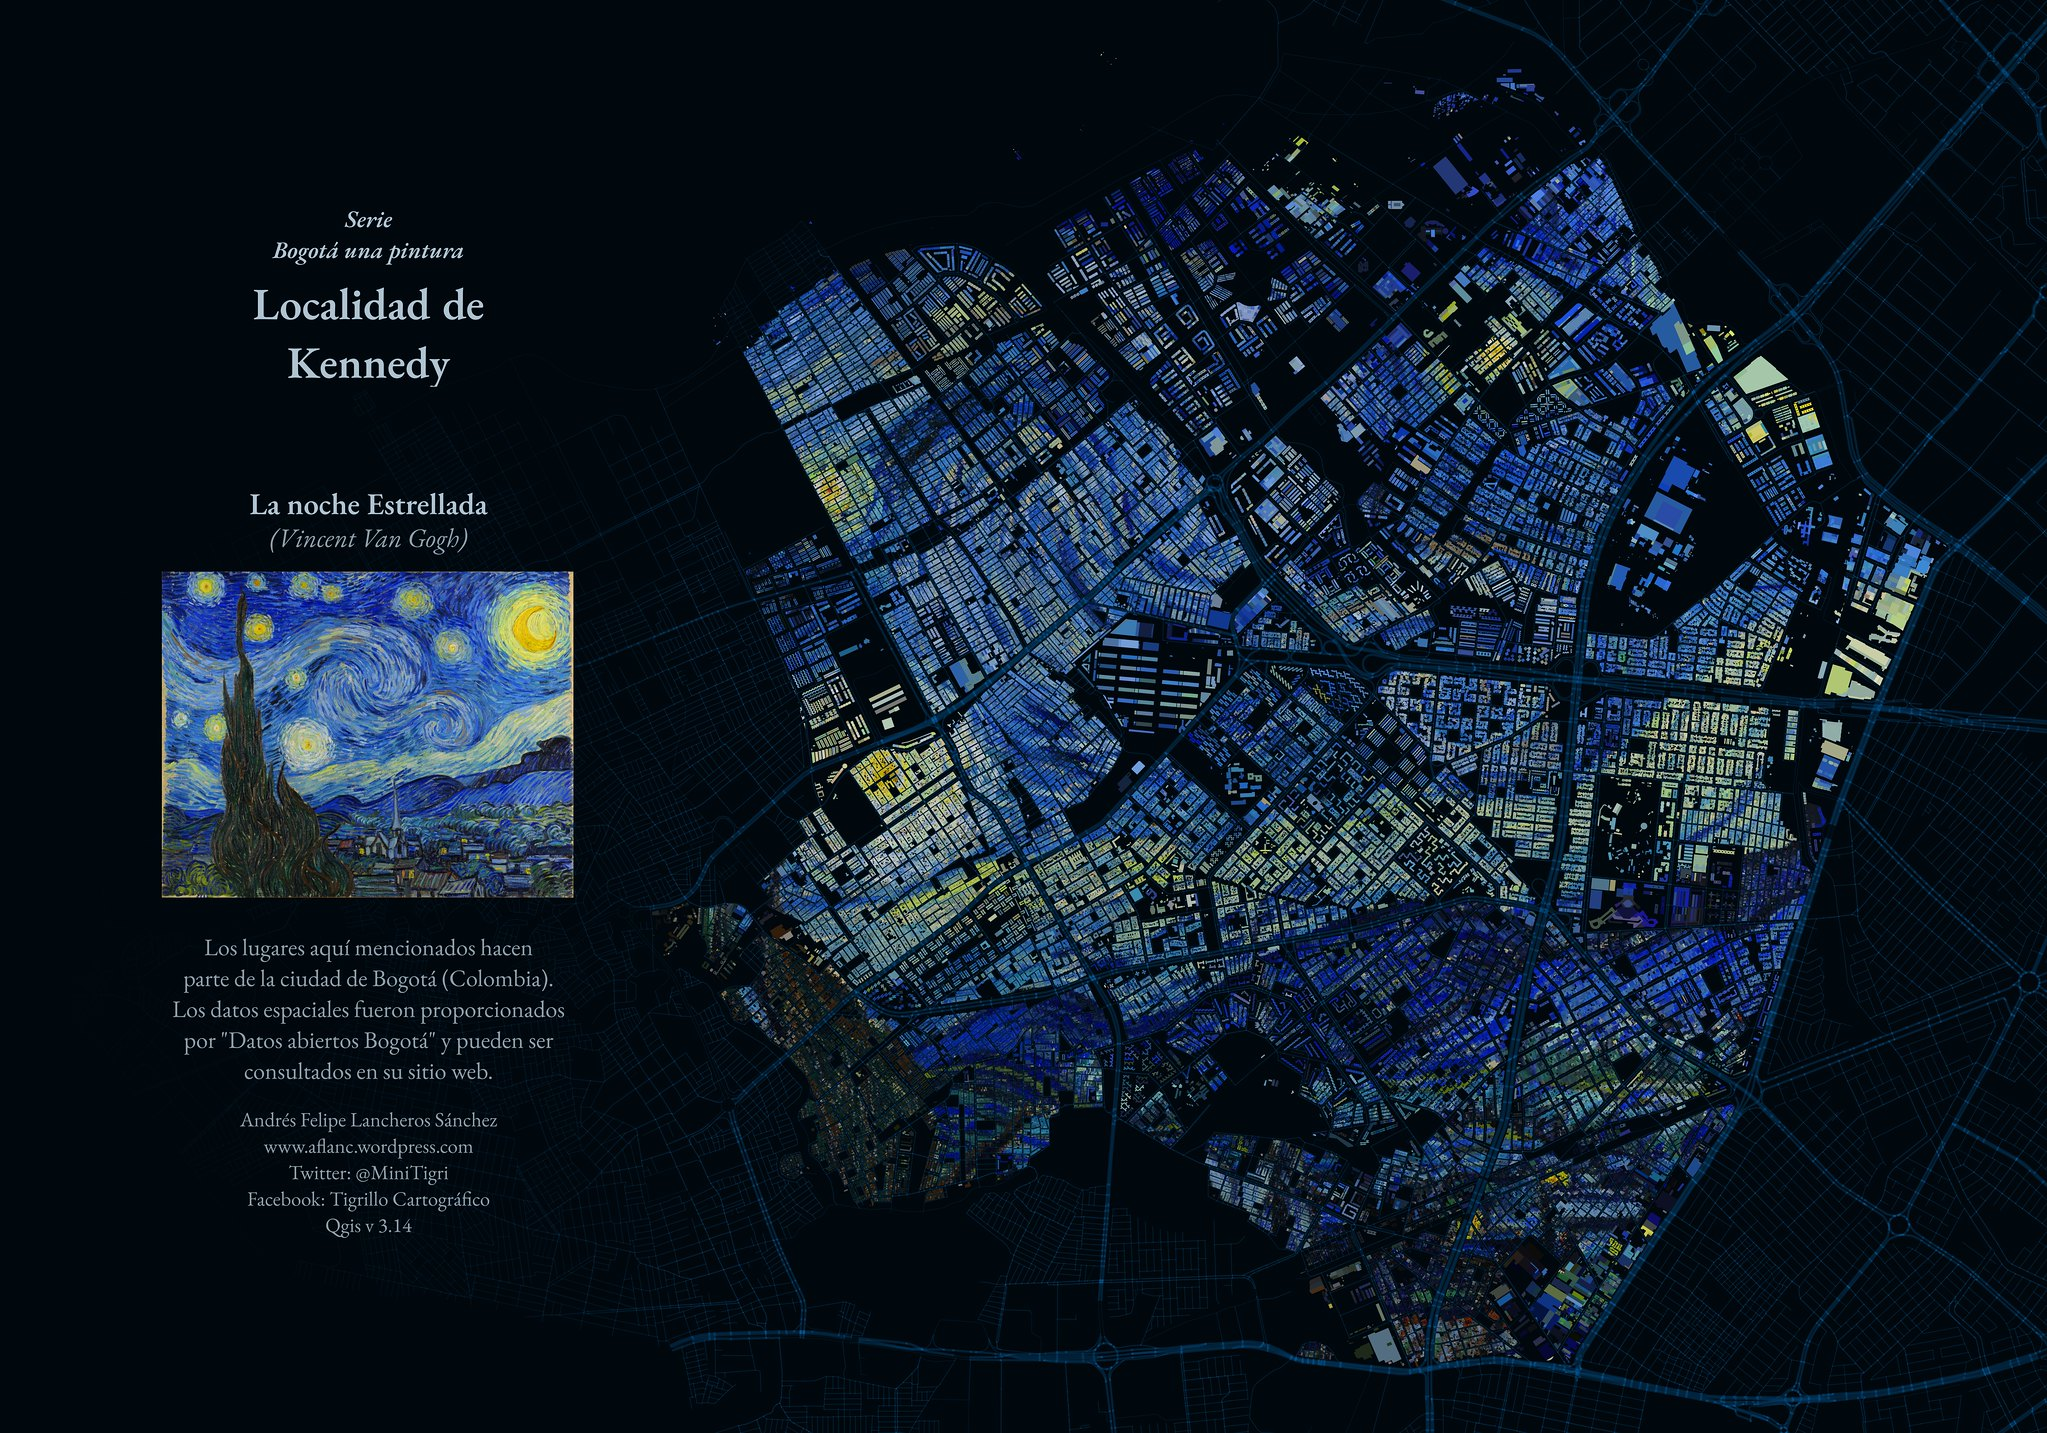
\includegraphics{_bookdown_files/_main_files/figure-html/media/modulo1/sample-1.jpg}
\caption{Mapa de Bogotá, Colômbia no estilo Noite Estrelada}
\end{figure}

Este próximo mapa (\url{https://flic.kr/p/2jAsphv}) mostra dados de rastreamento de tempestade da NOAA (o órgão de metereologia do governo dos EUA) entre 1851 e 2020 feitos por Fajr Alim.

\begin{figure}
\centering
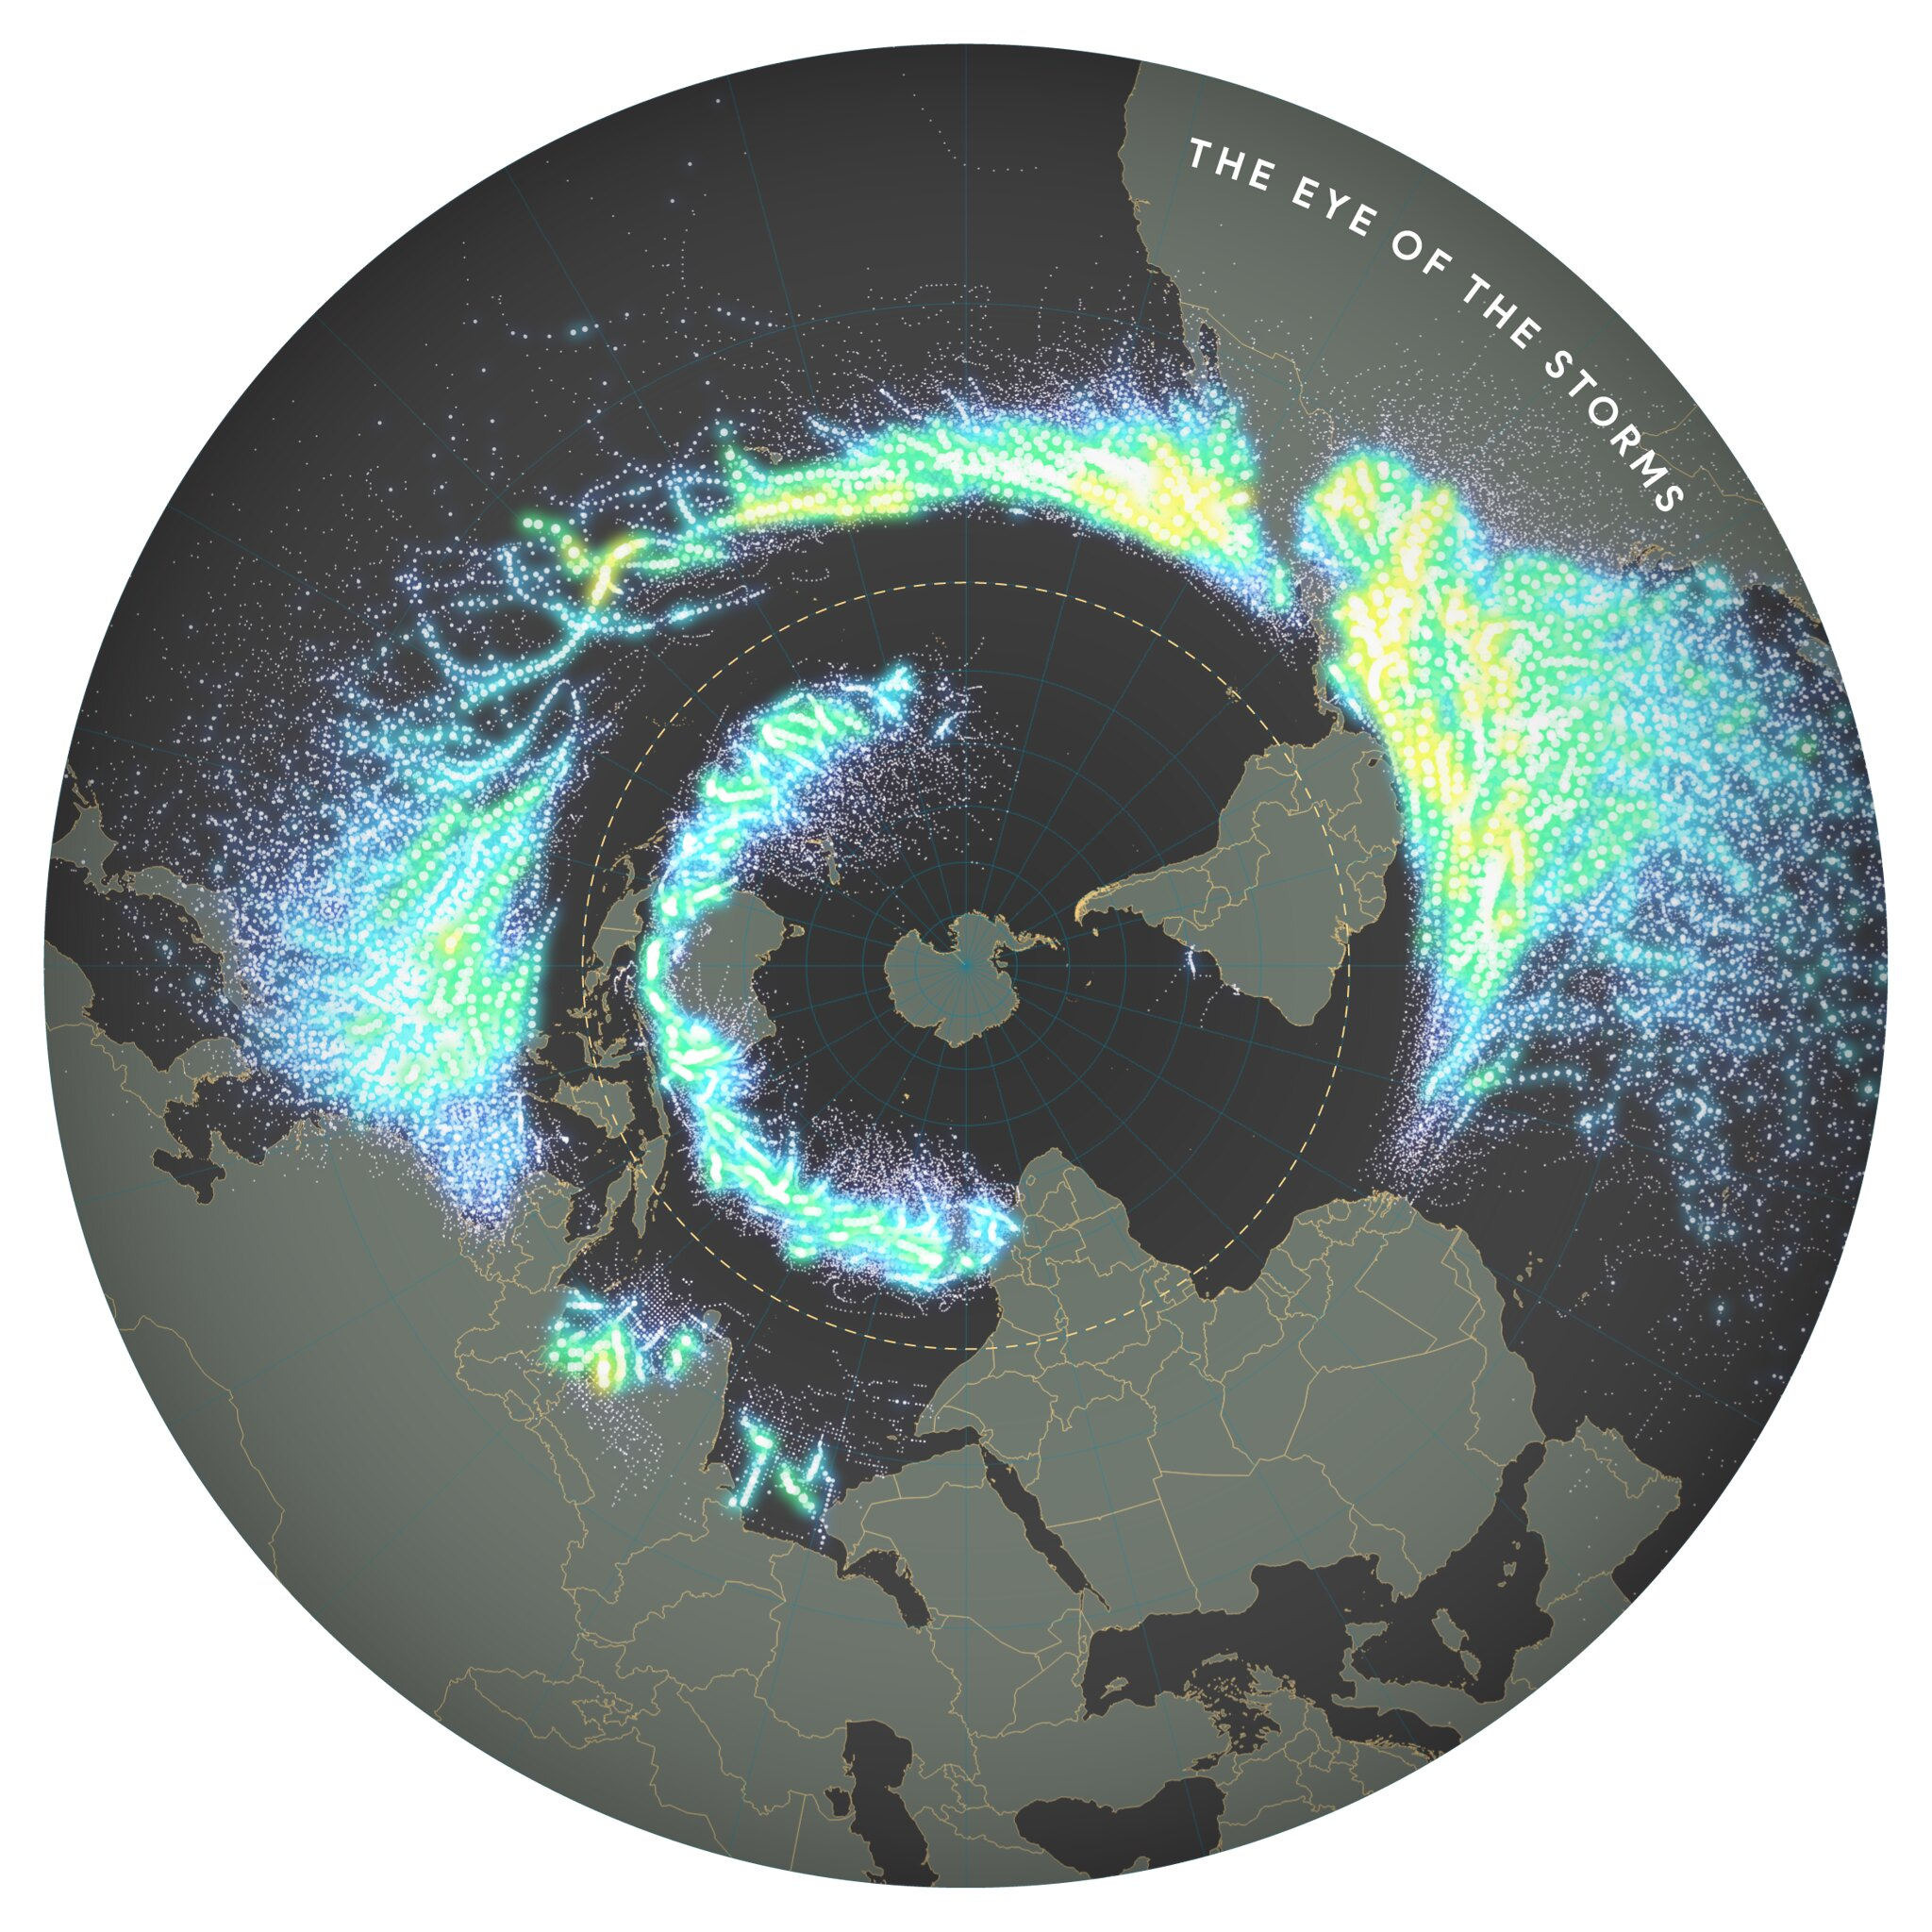
\includegraphics{_bookdown_files/_main_files/figure-html/media/modulo1/sample-2.jpg}
\caption{Dados de rastreamento de tempestade entre 1851 a 2020}
\end{figure}

Este próximo (\url{https://flic.kr/p/FA9TiR}) é um mapa da Ilha Kerguelen, feito por Heinrich Lingnau Schneider.

\begin{figure}
\centering
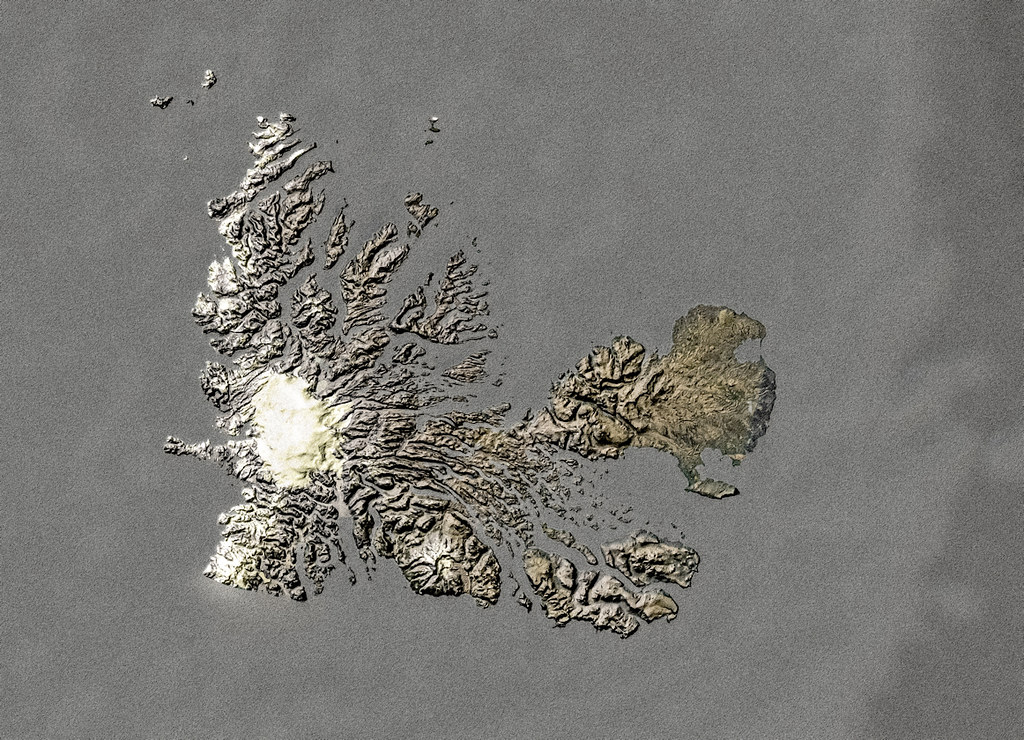
\includegraphics{_bookdown_files/_main_files/figure-html/media/modulo1/sample-3.jpg}
\caption{Mapa da Ilha Kerguelen}
\end{figure}

Este último (\href{https://flic.kr/p/v2kqVzsg}{https://flic.kr/p/2kqVzsg}) é de tentativas de arremessos de quadra e pontos marcados por tentativa durante a temporada 81 do Torneio de Basquete Masculino UAAP em as Filipinas por Ben Hur Pintor.

\begin{figure}
\centering
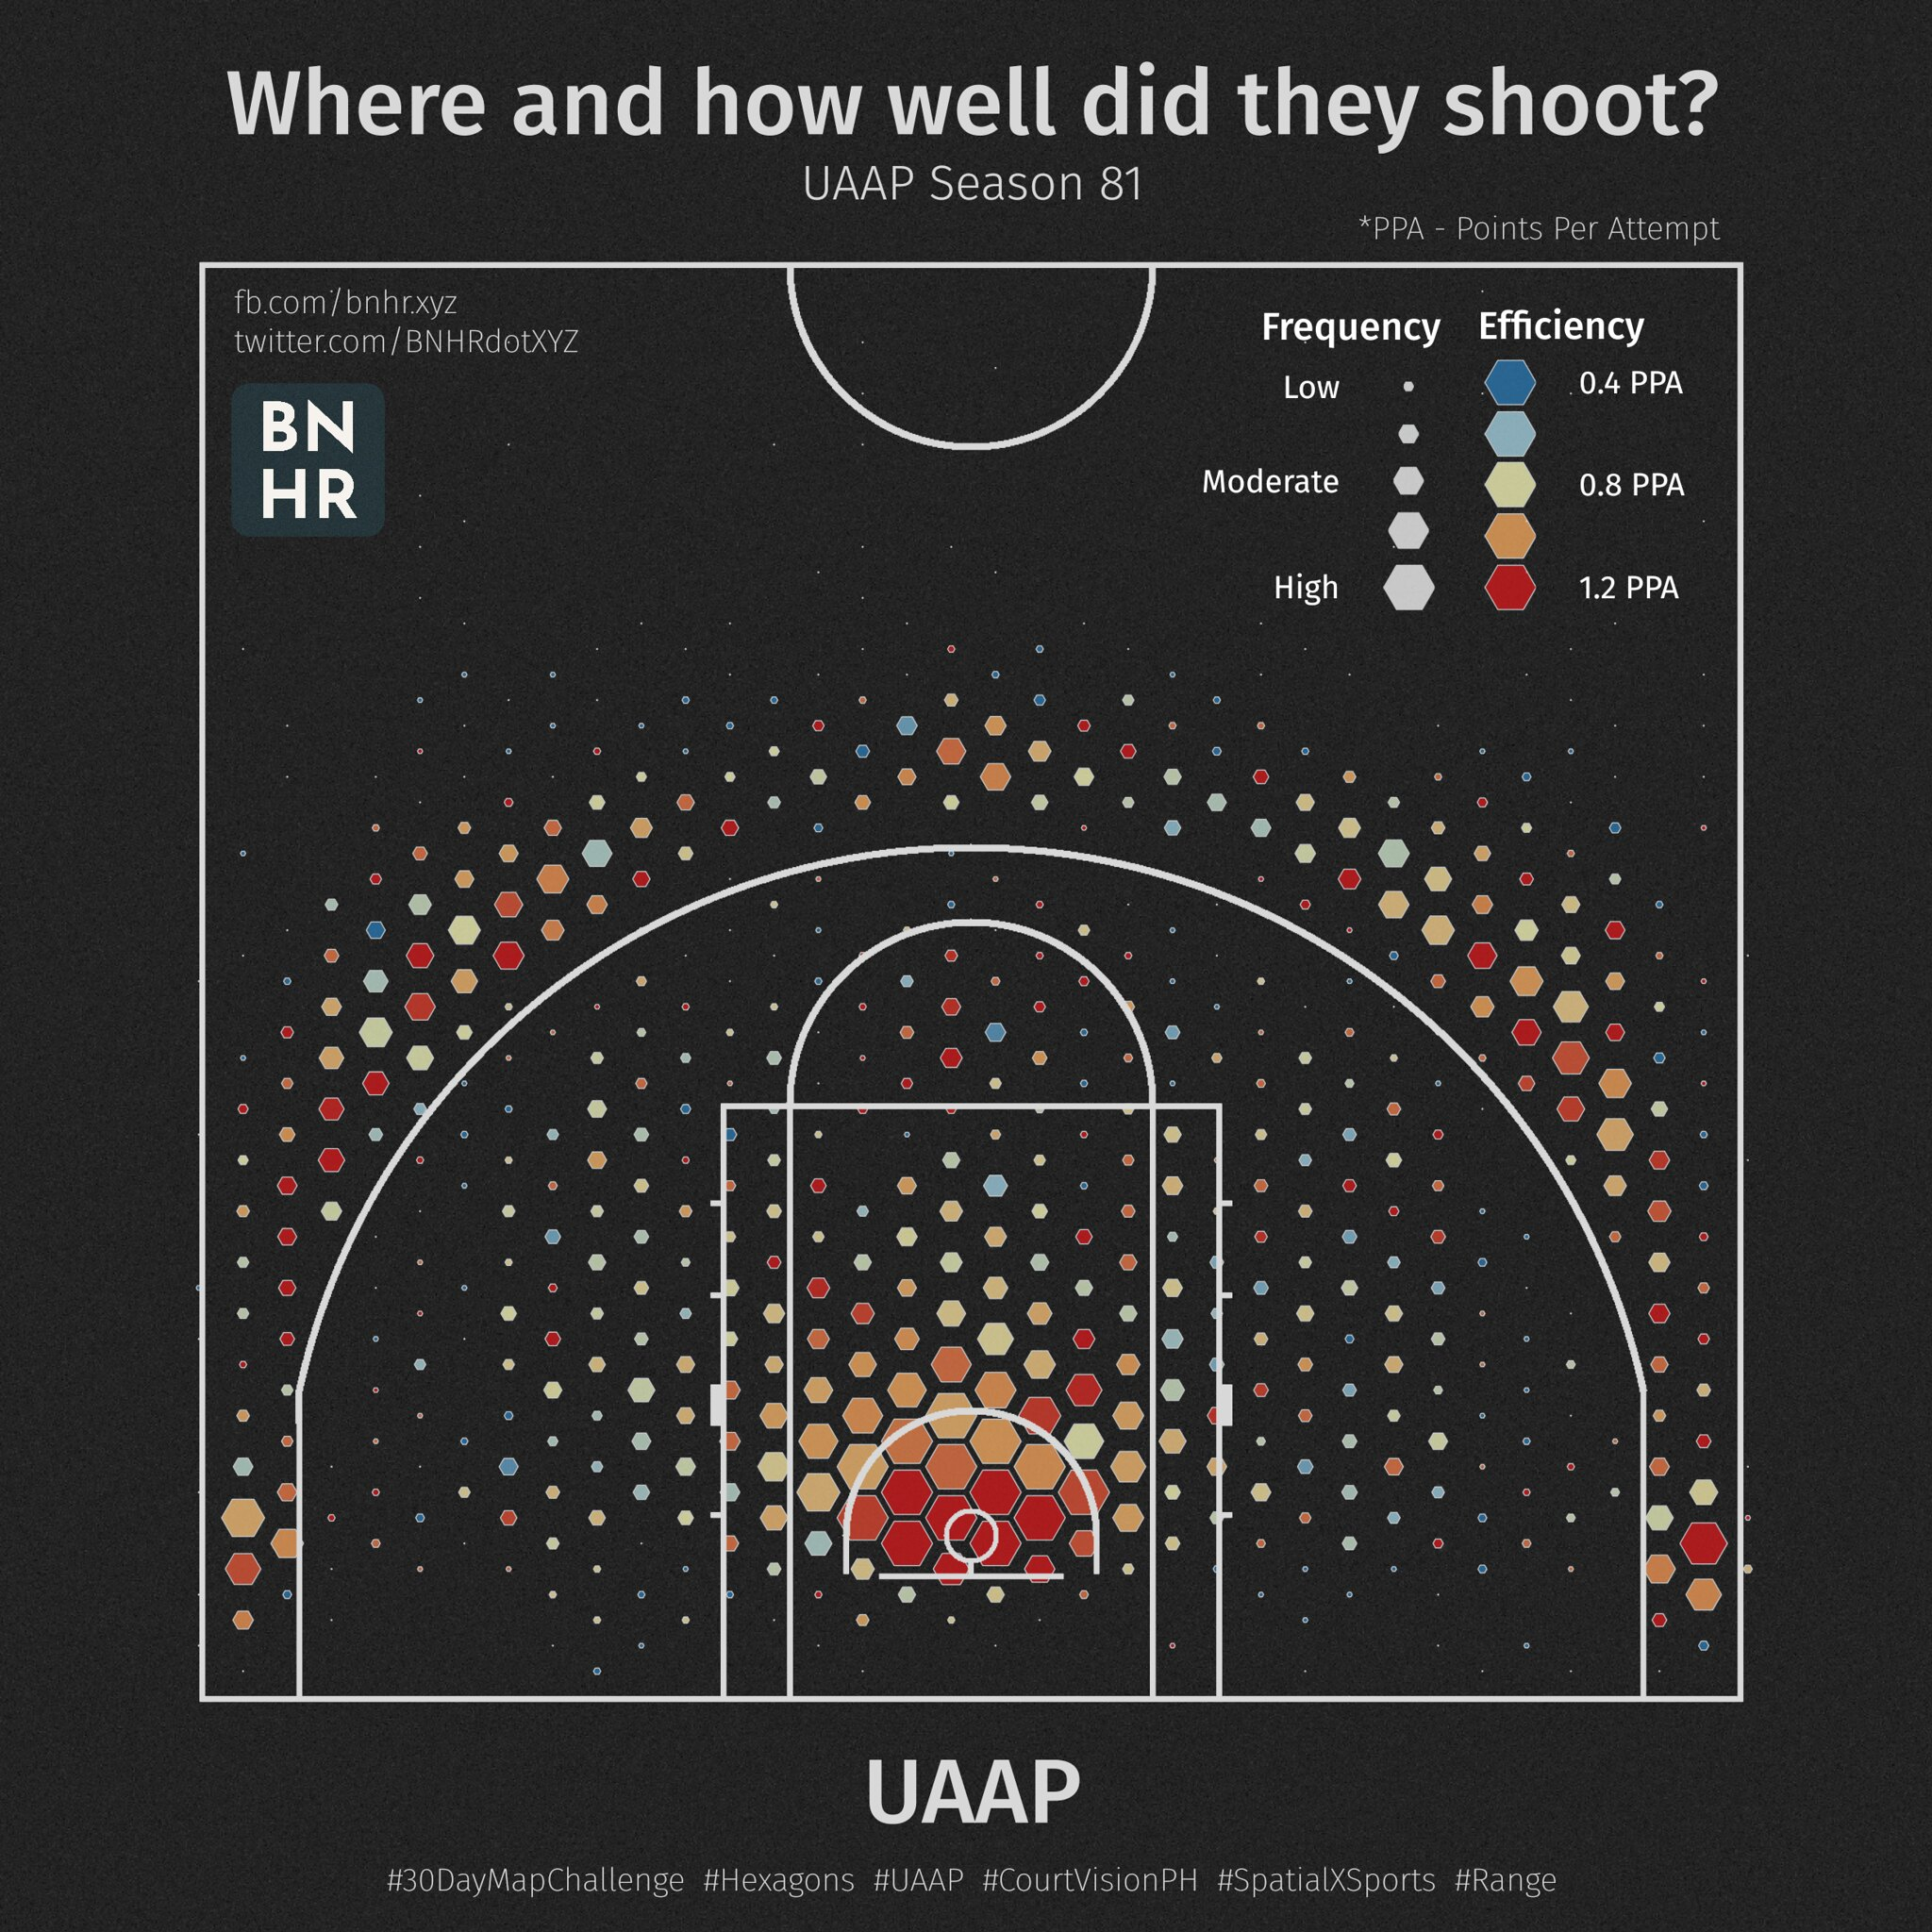
\includegraphics{_bookdown_files/_main_files/figure-html/media/modulo1/sample-4.jpg}
\caption{Tentativas de arremessos de quadra e pontos marcados na temporada 81 do UAAP}
\end{figure}

O que todos esses mapas têm em comum? Todos eles foram feitos usando o QGIS.

\hypertarget{detalhamento-dos-conceitos}{%
\section{Detalhamento dos conceitos}\label{detalhamento-dos-conceitos}}

Os mapas mostrados acima foram todos criados no QGIS (\url{https://qgis.org/en/site/}), um Sistema de Informação Geográfica (SIG, ou GIS) gratuito e de código aberto. O QGIS pode ser usado com todos os tipos de dados espaciais (como dados de basquete no último exemplo) e não apenas com dados geoespaciais relacionados à Terra.

As pessoas são capazes de criar mapas maravilhosos e surpreendentes, como os exemplos acima, porque o QGIS é gratuito, de código aberto e possui recursos poderosos de gerenciamento de dados, análise e apresentação.

\hypertarget{conteuxfado-principal-1}{%
\section{Conteúdo principal}\label{conteuxfado-principal-1}}

\hypertarget{tuxedtulo-da-fase-1-introduuxe7uxe3o-ao-qgis-e-uxe0-interface-do-qgis}{%
\subsection{Título da fase 1: Introdução ao QGIS e à interface do QGIS}\label{tuxedtulo-da-fase-1-introduuxe7uxe3o-ao-qgis-e-uxe0-interface-do-qgis}}

\hypertarget{o-que-uxe9-o-qgis}{%
\subsubsection{\texorpdfstring{\textbf{O que é o QGIS}}{O que é o QGIS}}\label{o-que-uxe9-o-qgis}}

\textbf{QGIS}, conhecido como Quantum GIS antes de seu lançamento 2.X, é um Sistema de Informação Geoespacial (GIS) maduro, multiplataforma, gratuito e de código aberto.

É um GIS de nível enterprise que possui recursos para coletar, armazenar, analisar, apresentar e gerenciar dados espaciais e não espaciais. Ele também se integra bem com outras tecnologias geoespaciais existentes e serve como parte integrante de qualquer pilha (stack) FOSS4G (Software Livre e de Código Aberto para Geoespacial).

Por ser multiplataforma, o QGIS pode ser executado em GNU / Linux, macOS, Windows e até mesmo Android.

\hypertarget{ciclo-de-lanuxe7amento-e-versuxf5es}{%
\subsubsection{\texorpdfstring{\textbf{Ciclo de lançamento e versões}}{Ciclo de lançamento e versões}}\label{ciclo-de-lanuxe7amento-e-versuxf5es}}

Os lançamentos e o desenvolvimento do QGIS seguem um cronograma / roteiro baseado no tempo (\href{https://www.qgis.org/en/site/\%20getinvolved\%20/\%20development\%20/\%20roadmap.html}{https://www.qgis.org/en/site/getinvolved/development/roadmap.html}).

Uma versão do QGIS é especificada por três números (X.Y.Z). Por exemplo, QGIS 3.16.4.

\begin{itemize}
\tightlist
\item
  X refere-se à versão principal. Neste caso, QGIS 3.
\item
  Y refere-se à versão de lançamento. Neste caso, a versão 16. As versões de lançamento são sempre números pares, pois os números ímpares são reservados para versões de desenvolvimento.
\item
  Z refere-se ao Point Release (PR) dessa versão. Para 3.16.4, isso significa que é o quarto ponto de lançamento da versão 3.16.
\end{itemize}

Existem três ramificações (ou branches) principais do QGIS que os usuários podem instalar. Estas são a ramificação \textbf{Long Term Release (LTR)}, a ramificação \textbf{Latest Release (LR)} e a ramificação \textbf{Development (Nightly)}.

\begin{itemize}
\tightlist
\item
  \textbf{Long Term Release (LTR)} tem esse nome porque é mantido e recebe correções de bug até o próximo LTR ser lançado. Atualmente, isso significa um (1) ano. Em fevereiro de 2021, o LTR atual é 3.16.4. Está programado para ser substituído pelo QGIS 3.22.4 em fevereiro de 2022.
\item
  \textbf{Última versão (LR)} refere-se a versão de lançamento do QGIS que contém os recursos mais recentes ou mais recentes. Um novo LR é lançado a cada quatro (4) meses. Por exemplo, um novo LR 3,18 foi lançado em fevereiro de 2021. O próximo LR (3.20) será lançado 4 meses a partir de agora, ou seja, em junho de 2021. Atualmente, cada terceiro LR se torna o próximo LTR. Por exemplo, o LTR de fevereiro de 2021 é a versão 3.16. O terceiro LR de 3.16 é 3.22, portanto, o próximo LTR será baseado na versão de lançamento 3.22.
\item
  \textbf{Development / Nightly} é baseado na versão mais recente do código-fonte QGIS, mas é útil se você deseja testar, depurar ou ajudar no desenvolvimento do QGIS.
\end{itemize}

Então, qual versão você deve usar? Depende. Se você precisa de uma versão que é mantida por mais tempo e não precisa necessariamente de novos recursos à medida que são lançados, a versão LTR pode ser a versão para você. Se você precisa dos recursos mais recentes e não se importa em fazer uma atualização a cada poucos meses, a versão LR pode ser ideal para você. Às vezes, também é bom dar uma olhada nas versões de desenvolvimento ou noturnas, especialmente se você estiver curioso ou animado com os próximos recursos do QGIS.

Para obter mais informações, visite: \href{https://bnhr.xyz/2020/10/26/\%20about-qgis-versions-release-cycle-english.html}{https://bnhr.xyz/2020/10/26/about-qgis-versions-release-cycle-english.html}

\hypertarget{exemplos-de-mapas-qgis}{%
\subsubsection{\texorpdfstring{\textbf{Exemplos de mapas QGIS}}{Exemplos de mapas QGIS}}\label{exemplos-de-mapas-qgis}}

\begin{figure}
\centering
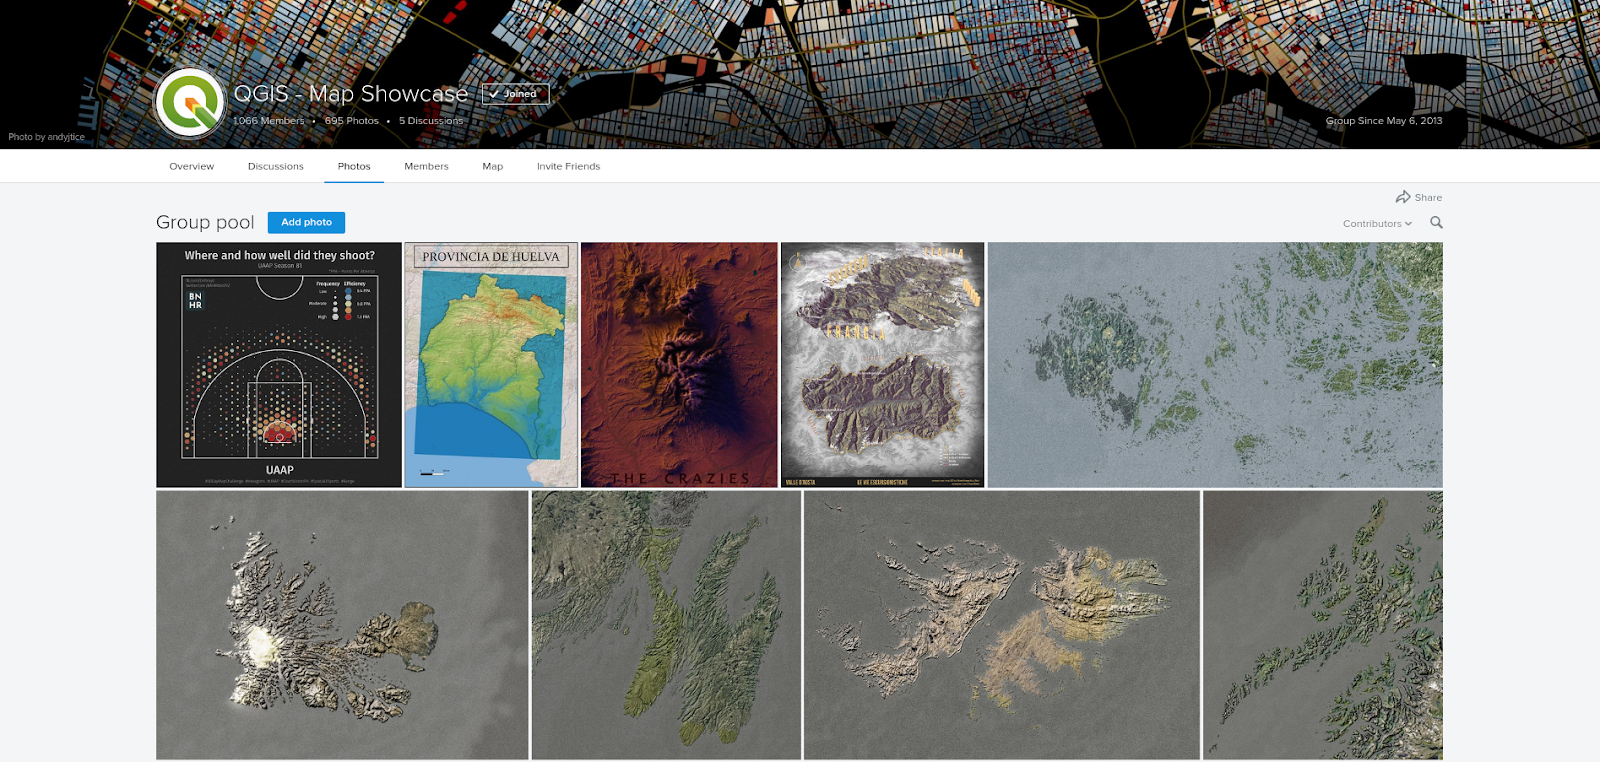
\includegraphics{_bookdown_files/_main_files/figure-html/media/modulo1/qgis-map-showcase.png}
\caption{QGIS Map Showcase}
\end{figure}

Figura 1.1. Demonstração do mapa QGIS

Para mais mapas criados com o QGIS, visite: \href{https://www.flickr.com/groups/2244553@N22/\%20piscina/com/50355460063/}{https://www.flickr.com/groups/2244553@N22/pool/with/50355460063/}

\hypertarget{instalando-o-qgis}{%
\subsubsection{\texorpdfstring{\textbf{Instalando o QGIS}}{Instalando o QGIS}}\label{instalando-o-qgis}}

QGIS é multiplataforma e funciona em Linux, Windows e macOS. Sendo de código aberto, você pode construir e instalar o QGIS a partir de seu código-fonte, disponível em \url{https://github.com/qgis/QGIS/}.

Instaladores e instruções de instalação também estão disponíveis em \url{https://qgis.org/en/site/forusers/download.html} ou \href{https://qgis.org/en/site/forusers/alldownloads.html}{https: //qgis.org/en/site/forusers/alldownloads.html}.

Para \textbf{Linux (ou GNU / Linux)}, o QGIS geralmente está disponível no gerenciador de pacotes de sua distribuição. Para usuários Debian / Ubuntu, o QGIS tem repositórios para os ramos LR, LTR e Desenvolvimento (Development), bem como versões do QGIS com dependências do PPA ubuntugis-unstable. O QGIS também está disponível como pacote Flatpak ou no Conda.

Para \textbf{Windows}, os usuários podem escolher entre o instalador de rede OSGeo4W ou os instaladores independentes. Há um instalador independente para a versão LTR e LR.

Os instaladores autônomos são os mais fáceis de instalar e são recomendados para iniciantes. Várias versões do QGIS podem ser instaladas em seu computador ao mesmo tempo. Isso significa que você pode ter ambas as versões QGIS 3.16 e 3.18 instaladas.

O OSGeo4W Network Installer é um pouco mais avançado e complexo do que os instaladores autônomos, mas também oferece a capacidade de atualizar e atualizar sua versão do QGIS no local, o que significa que você não precisará desinstalar uma versão mais antiga se quiser instalar um mais novo.

Em alguns casos, você precisará de direitos de administrador para instalar o QGIS, portanto, se estiver instalando em um computador onde o seu usuário não possui direitos de administrador, pode ser necessário pedir ao seu administrador de TI ou escritório para instalar o QGIS para você.

A instalação no Windows também vem com QGIS com GRASS (outro GIS Livre e de Código Aberto).

Observe que o QGIS está \href{https://blog.qgis.org/2020/10/15/phasing-out-32-bit-support-in-qgis/}{removendo lentamente o suporte de 32 bits para Windows}, então é melhor para instalar o QGIS em um computador que executa um sistema operacional de 64 bits.

Para o \textbf{macOS}, existem instaladores oficiais ``All-in-one'' assinados para macOS High Sierra (10.13) e mais recentes. O QGIS ainda não foi autenticado conforme exigido pelas regras de segurança do macOS Catalina (10.15). Na primeira inicialização, clique com o botão direito no ícone do aplicativo QGIS, segure a tecla Option e escolha Abrir.

\hypertarget{partes-da-interface-do-qgis}{%
\subsubsection{\texorpdfstring{\textbf{Partes da interface do QGIS}}{Partes da interface do QGIS}}\label{partes-da-interface-do-qgis}}

Depois de instalar o QGIS, você pode executá-lo ou abri-lo como faria com qualquer programa em seu computador. Ao abrir o QGIS, você será saudado com a Interface do Usuário (IU, ou UI em inglês) padrão que se parecerá com a abaixo.

\begin{figure}
\centering
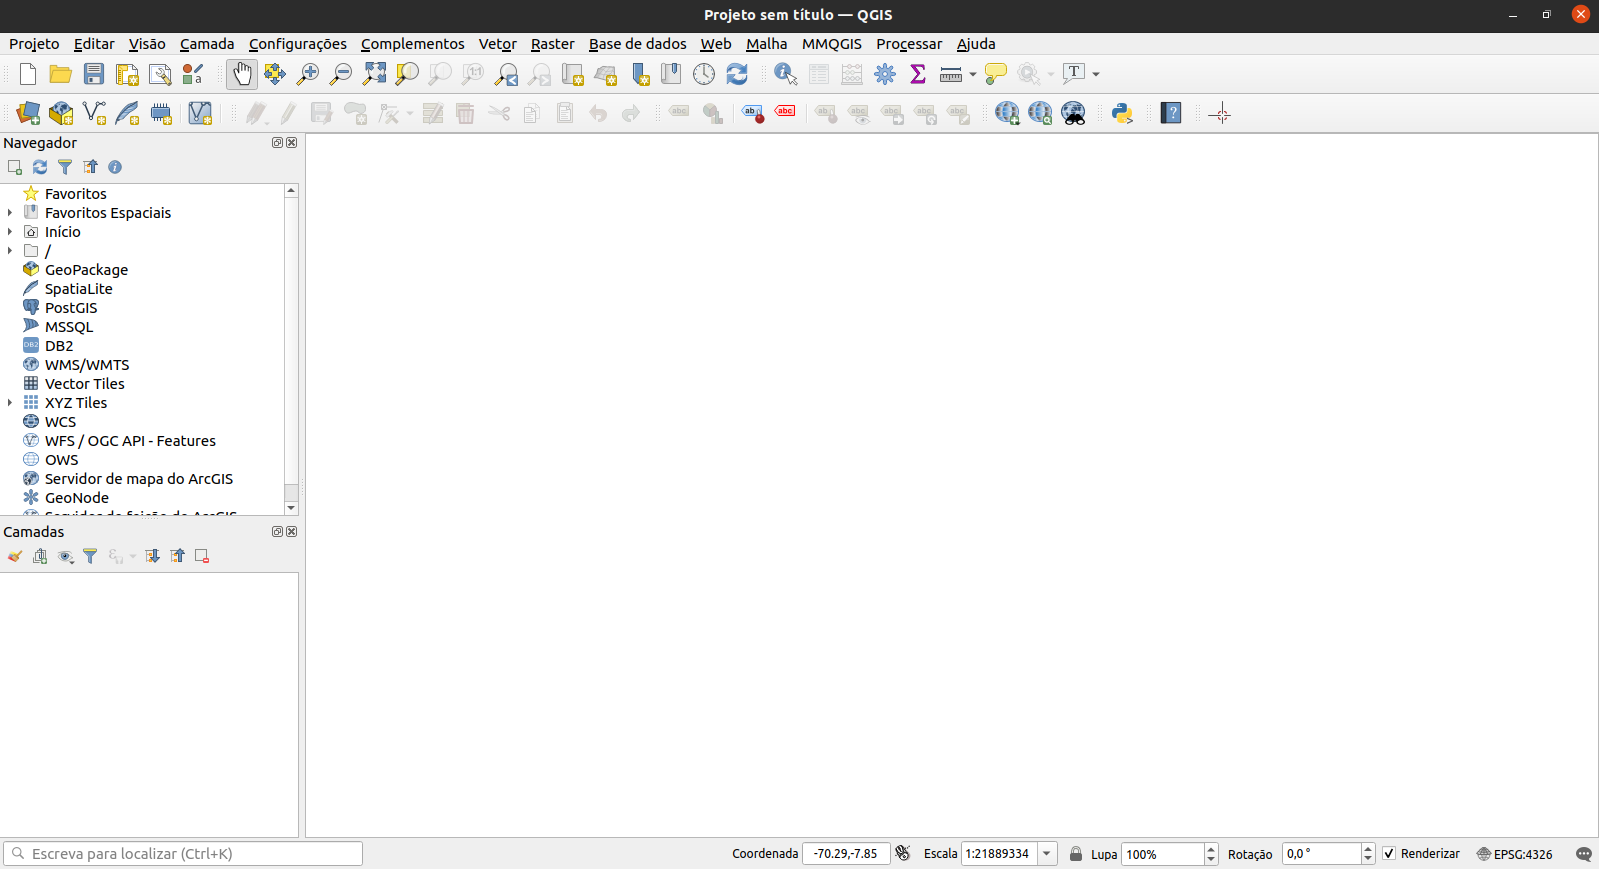
\includegraphics{_bookdown_files/_main_files/figure-html/media/modulo1/qgis-interface.png}
\caption{A interface QGIS}
\end{figure}

Figura 1.2. A interface QGIS em uma nova instalação

Existem seis partes principais da interface de usuário do QGIS - barra de menu, tela do mapa, barra de ferramentas, painéis, barra de status e localizador.

No centro da interface está uma tela de mapa. Painéis e barras de ferramentas podem ser posicionados em torno dessa tela. Os painéis também podem ser acoplados para criar um painel com várias abas. Existem também outras partes da interface, como a interface Python, janelas de complemento, etc.

\textbf{Barra de menus} - a barra de menus é um menu hierárquico simples que fornece acesso às funções e comandos do QGIS. Geralmente está localizado na parte superior da interface.

\textbf{Tela do mapa} - a tela do mapa é onde as camadas carregadas no QGIS são mostradas. Este é também o local onde os filtros, seleções, e simbologias criadas pelo usuário são refletidas. Mais de uma tela de mapa pode estar presente a qualquer momento. Um usuário pode aplicar zoom, panorâmica e até mesmo girar a tela do mapa. Uma tela de mapa também pode mostrar dados 3D.

\textbf{Barras de ferramentas} - as barras de ferramentas mostram botões de acesso fácil aos comandos, recursos, complementos do QGIS. Eles podem ser movidos e encaixados na tela do mapa. A lista de barras de ferramentas pode ser encontrada, ativada e desativada na barra de menus em \textbf{Exibir ‣ Barras de ferramentas}. Exemplos de barras de ferramentas são a barra de ferramentas de atributos e a barra de ferramentas de digitalização.

\textbf{Painéis} - os painéis são semelhantes às barras de ferramentas, mas, em vez de botões, fornecem uma interface para funções e recursos mais complexos. O painel de camadas e o painel do navegador são dois exemplos. Semelhante às barras de ferramentas, eles podem ser movidos e encaixados na tela do mapa. A lista de painéis pode ser encontrada, ativada e desativada na barra de menus em \textbf{Exibir ‣ Painéis}.

\textbf{Barra de status} - a barra de status é comumente encontrada na parte inferior da interface e mostra informações relevantes, como CRS, escala, notificações, etc.

\textbf{Barra Localizadora} - a barra Localizadora é encontrada no canto inferior esquerdo da interface do QGIS. Ele permite que o usuário acesse facilmente camadas, campos, algoritmos de processamento e outras funcionalidades no QGIS. Este é um dos recursos mais poderosos do QGIS.

\begin{figure}
\centering
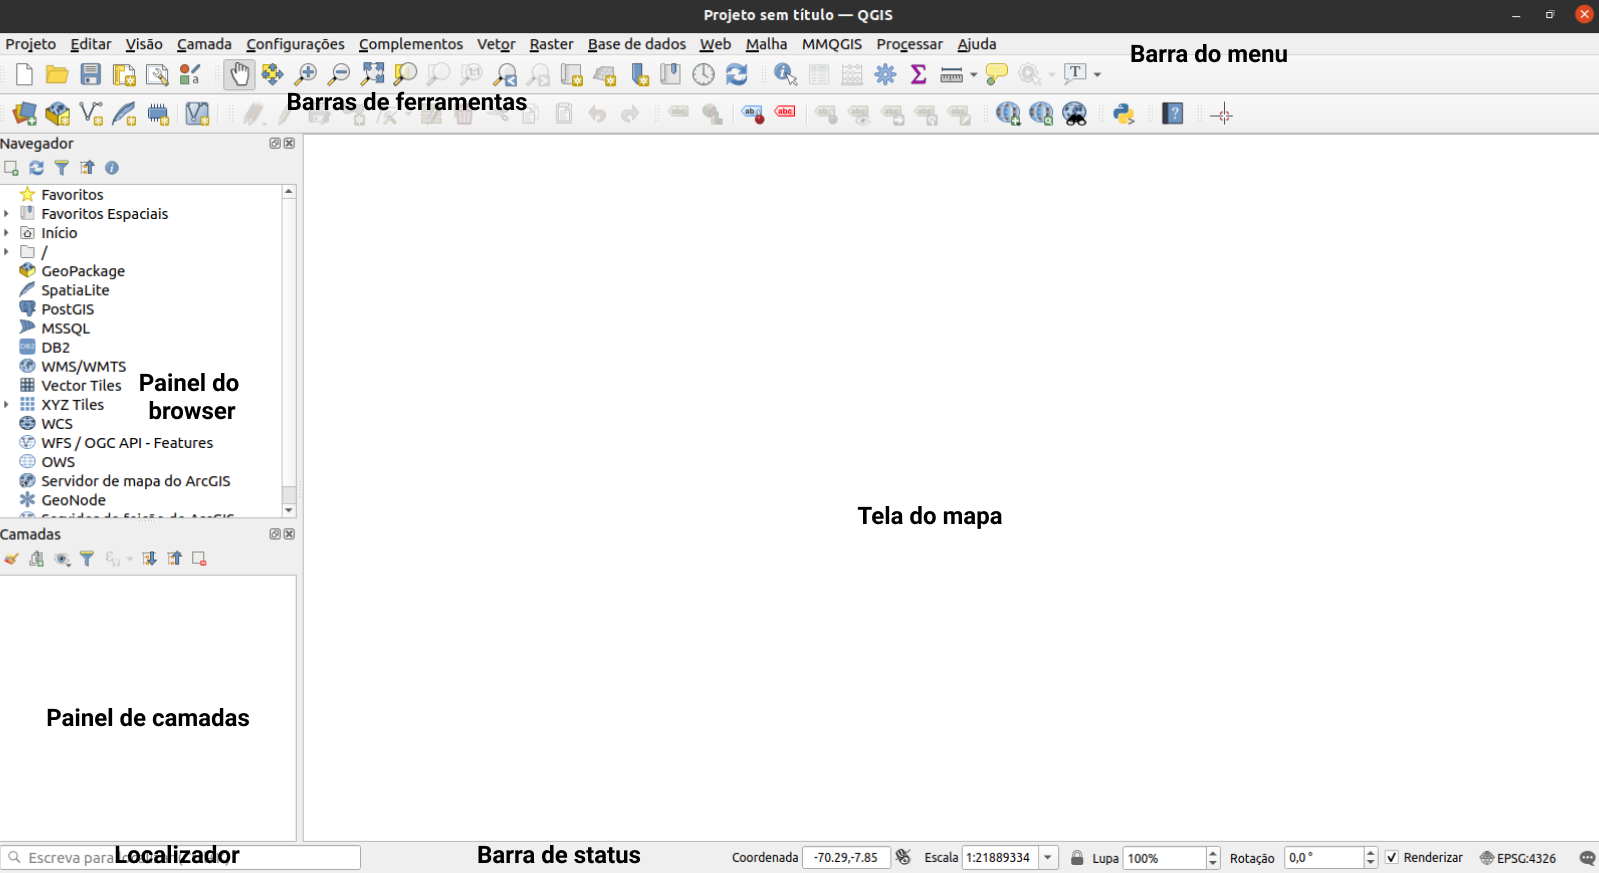
\includegraphics{_bookdown_files/_main_files/figure-html/media/modulo1/qgis-interface-parts.png}
\caption{Partes da interface QGIS}
\end{figure}

Figura 1.3. Partes da interface QGIS

Uma das belezas do QGIS é a personalização ele que oferece aos seus usuários. Essa personalização começa com a interface do usuário. Ao editar algumas configurações e mover algumas partes da interface, você pode ter um QGIS semelhante a este abaixo:

\begin{figure}
\centering
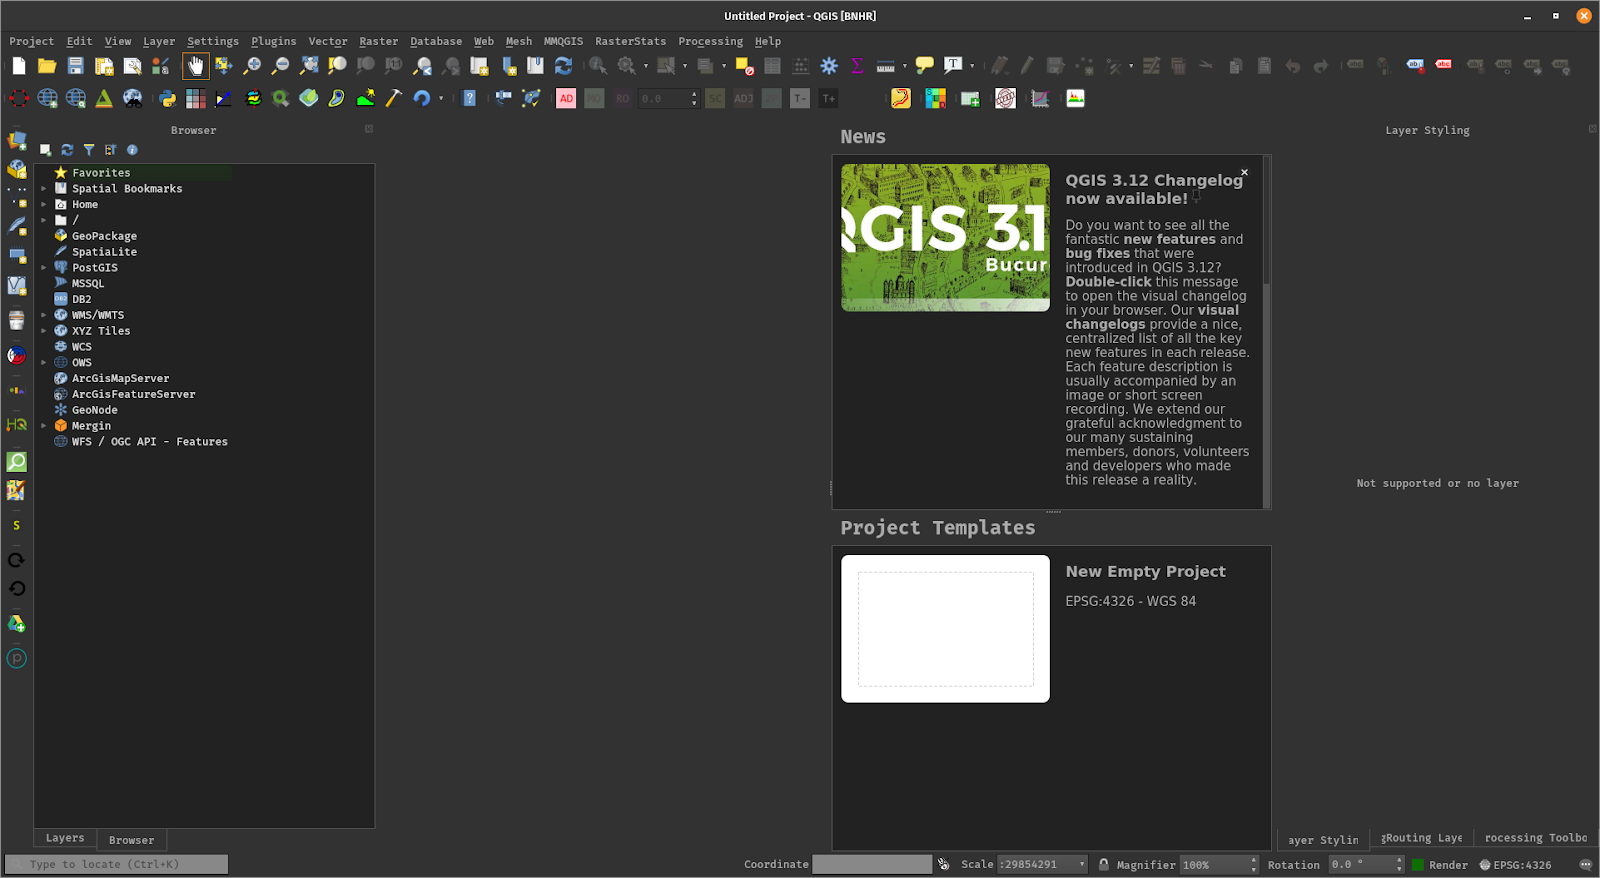
\includegraphics{_bookdown_files/_main_files/figure-html/media/modulo1/qgis-interface-custom.png}
\caption{Interface QGIS com algumas personalizações}
\end{figure}

Figura 1.4. A interface QGIS com algumas personalizações

\hypertarget{tutorial-exercuxedcio-1-mudando-a-aparuxeancia-e-layout-da-interface-qgis}{%
\subsubsection{\texorpdfstring{\textbf{Tutorial / Exercício 1: Mudando a aparência e layout da interface QGIS}}{Tutorial / Exercício 1: Mudando a aparência e layout da interface QGIS}}\label{tutorial-exercuxedcio-1-mudando-a-aparuxeancia-e-layout-da-interface-qgis}}

\begin{enumerate}
\def\labelenumi{\arabic{enumi}.}
\tightlist
\item
  Abra o \textbf{QGIS}
\item
  Clique no menu \textbf{Visão}
\end{enumerate}

\begin{figure}
\centering
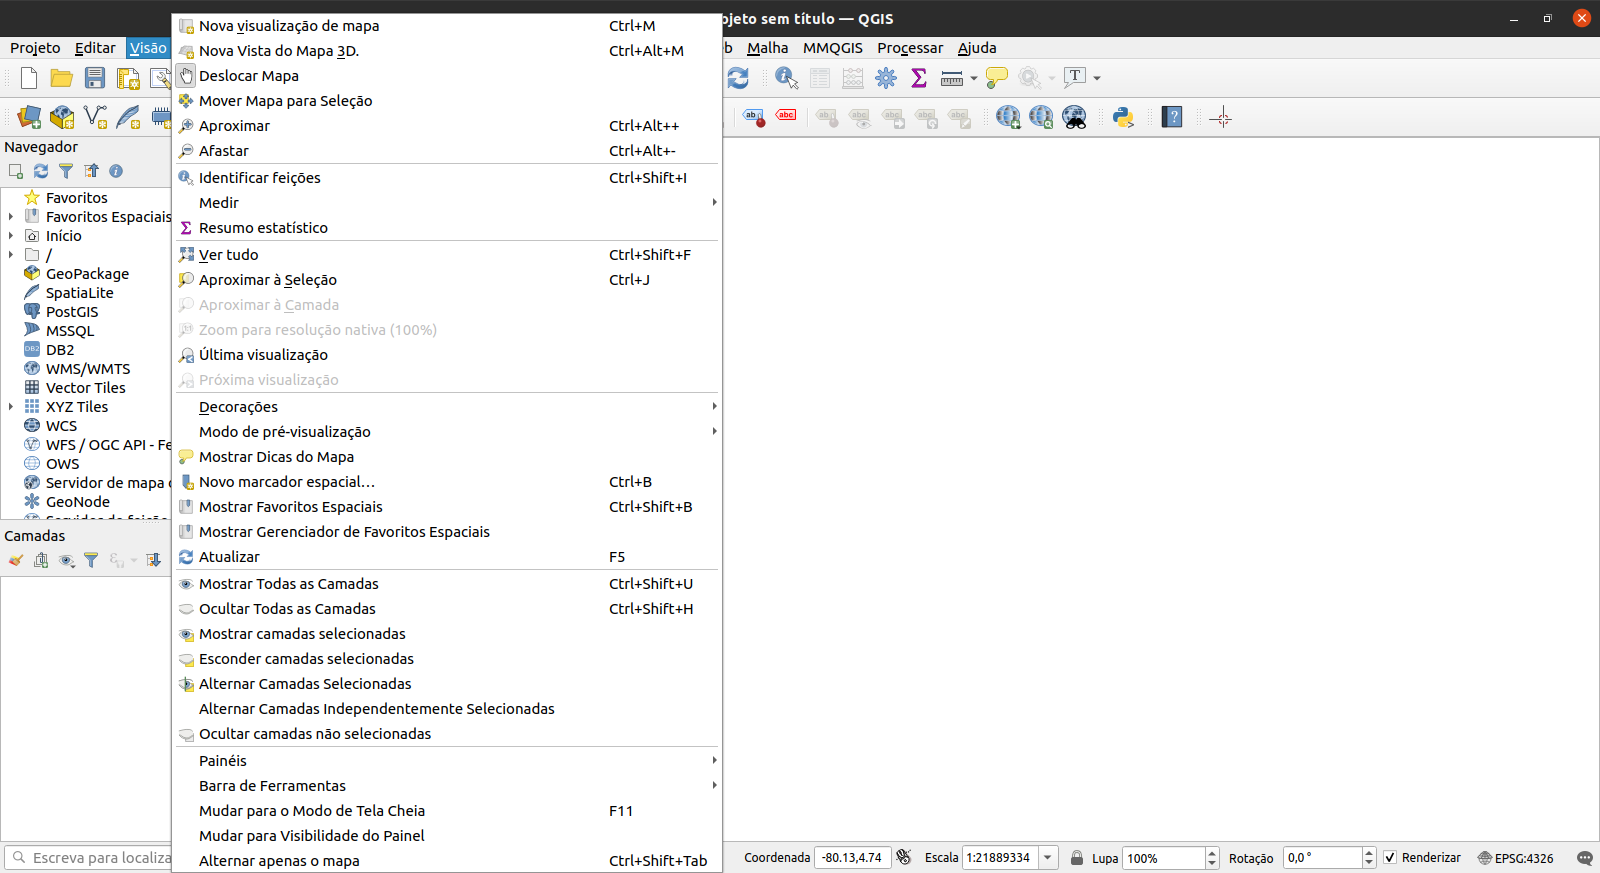
\includegraphics{_bookdown_files/_main_files/figure-html/media/modulo1/ex01-01.png}
\caption{Abra o QGIS e clique no menu Exibir}
\end{figure}

\begin{enumerate}
\def\labelenumi{\arabic{enumi}.}
\setcounter{enumi}{2}
\tightlist
\item
  Observe o menu \textbf{Painéis}
\end{enumerate}

\begin{figure}
\centering
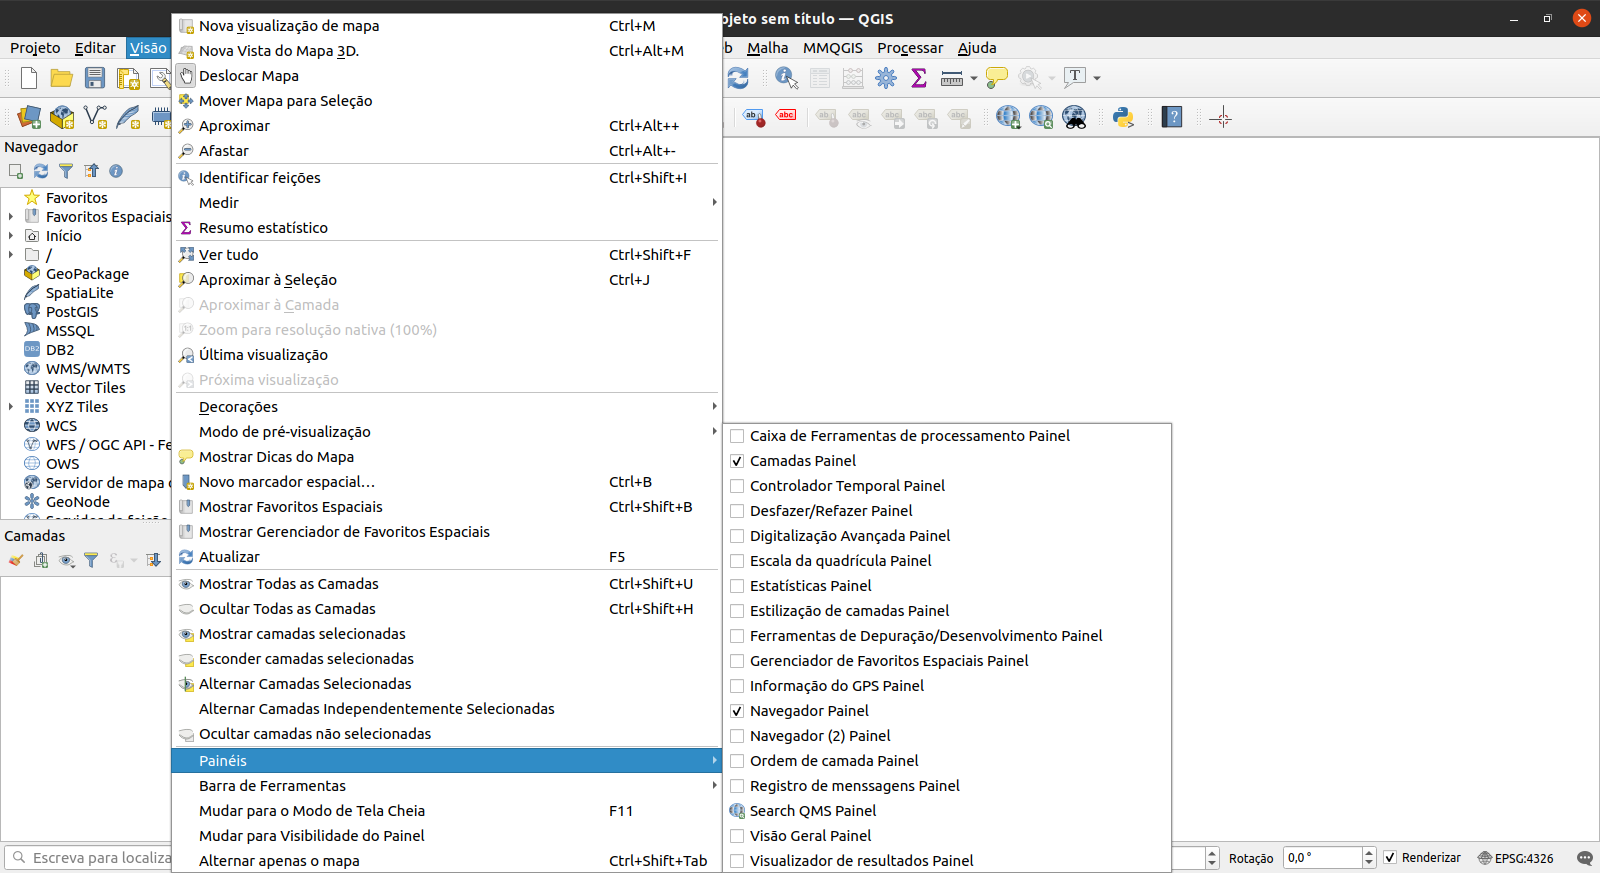
\includegraphics{_bookdown_files/_main_files/figure-html/media/modulo1/ex01-02.png}
\caption{Observe o menu Painéis}
\end{figure}

\begin{enumerate}
\def\labelenumi{\arabic{enumi}.}
\setcounter{enumi}{3}
\tightlist
\item
  Observe o menu \textbf{Barras de ferramentas}
\end{enumerate}

\begin{figure}
\centering
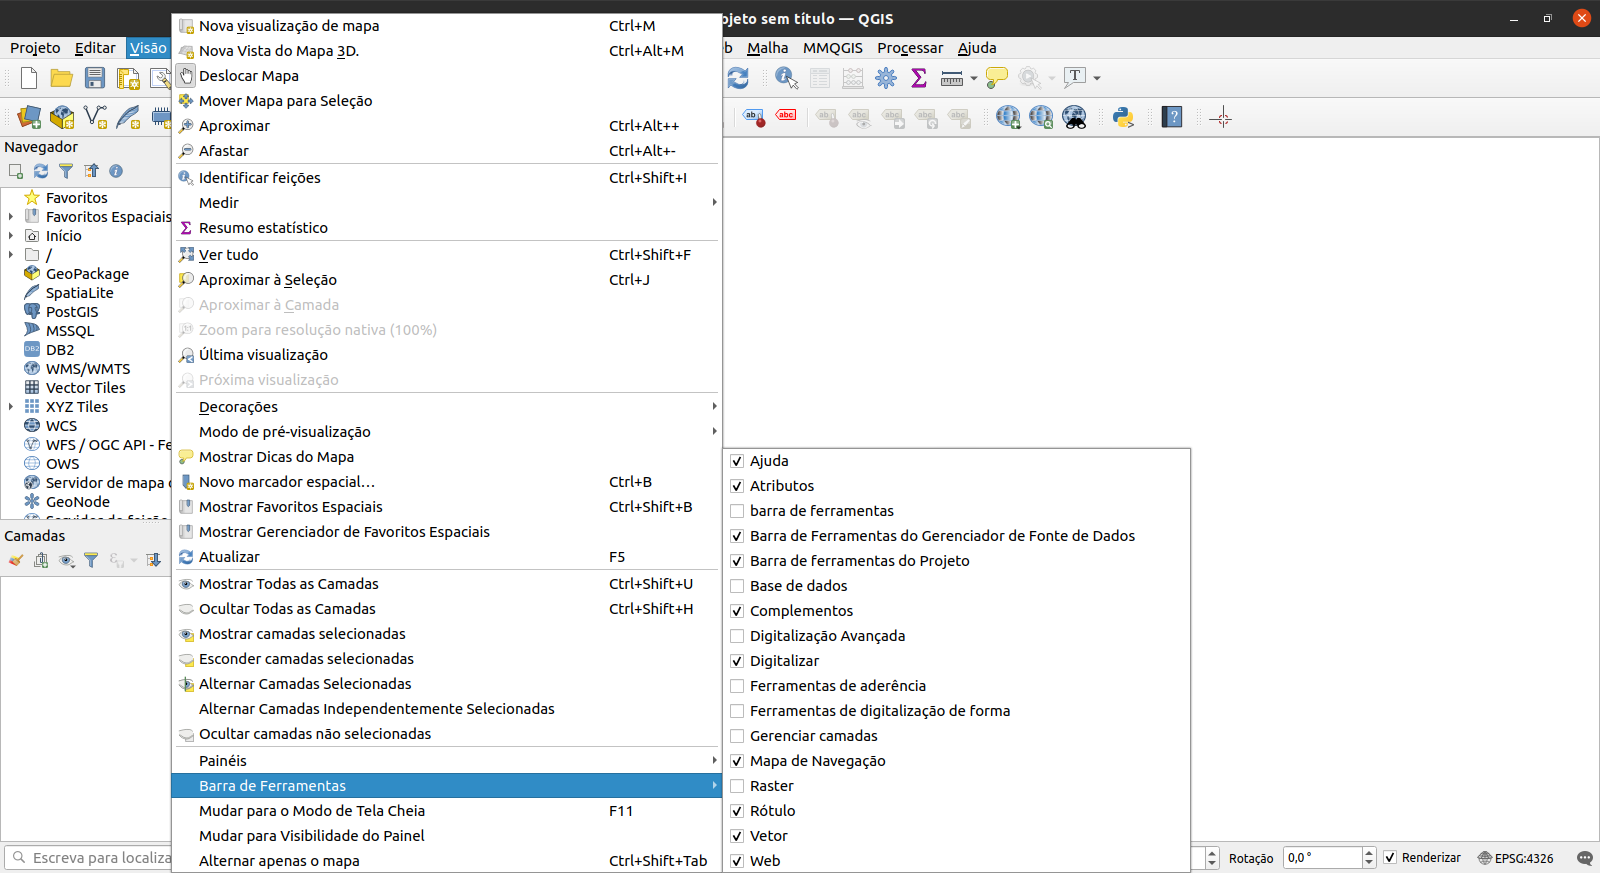
\includegraphics{_bookdown_files/_main_files/figure-html/media/modulo1/ex01-03.png}
\caption{Observe o menu Barras de ferramentas}
\end{figure}

\begin{enumerate}
\def\labelenumi{\arabic{enumi}.}
\setcounter{enumi}{4}
\tightlist
\item
  Selecione as \textbf{Barras de ferramentas} e \textbf{Painéis} que você deseja mostrar na interface do usuário. Alguns dos painéis úteis incluem \textbf{Estilização de camadas} e \textbf{Caixa de Ferramentas de Processamento}.
\item
  Mova as \textbf{Barras de Ferramentas} e \textbf{Painéis} para as posições que fizerem mais sentido para você
\end{enumerate}

\textbf{Resetando a interface QGIS}

Para redefinir sua tela para as configurações padrão, vá para \textbf{Configurações ‣ Opções ‣ Guia Sistema ‣ Configurações ‣ Botão Redefinir} e reinicie o QGIS.

\hypertarget{perguntas-do-questionuxe1rio-2}{%
\subsubsection{\texorpdfstring{\textbf{Perguntas do questionário}}{Perguntas do questionário}}\label{perguntas-do-questionuxe1rio-2}}

\begin{enumerate}
\def\labelenumi{\arabic{enumi}.}
\tightlist
\item
  Verdadeiro ou falso:

  \begin{enumerate}
  \def\labelenumii{\arabic{enumii}.}
  \tightlist
  \item
    Você pode ter várias telas de mapa - \textbf{\emph{Verdadeiro}}
  \item
    Você pode mostrar ou ocultar painéis e barras de ferramentas - \textbf{\emph{Verdadeiro}}
  \item
    Você só pode colocar painéis no lado esquerdo ou direito da tela do mapa - \textbf{\emph{Falso (você também pode colocar painéis acima ou abaixo da tela do mapa)}}
  \end{enumerate}
\end{enumerate}

\hypertarget{tuxedtulo-da-fase-2-complementos-complementos-qgis}{%
\subsection{Título da fase 2: Complementos (Complementos) QGIS}\label{tuxedtulo-da-fase-2-complementos-complementos-qgis}}

A capacidade de adicionar, criar e estender a funcionalidade do QGIS por meio de complementos (ou plug-ins) é um de seus recursos mais poderosos.

A partir do QGIS 3.16.3, existem mais de 700 complementos disponíveis para o usuário baixar e melhorar. Esses complementos variam do complexo ao simples.

Os complementos QGIS podem ser classificados como:

\begin{itemize}
\tightlist
\item
  \textbf{Complementos core} - integrado à sua versão do QGIS, não pode ser desinstalado
\item
  \textbf{Complementos externos} - manualmente instalados por meio de busca em um repositório externo (ou seja, QGIS Official Plugin Repository) ou através do código-fonte.
\end{itemize}

Os complementos podem ser instalados de três (3) maneiras:

\begin{enumerate}
\def\labelenumi{\arabic{enumi}.}
\tightlist
\item
  Através da caixa de diálogo Gerenciar e instalar complementos (\textbf{Complementos ‣ Gerenciar e instalar complementos})
\item
  Instalando do ZIP, que pode ser acessado na guia \textbf{Instalar do ZIP} na caixa de diálogo Gerenciar e instalar complementos.
\item
  Adicionando manualmente o código-fonte na pasta de complementos do seu perfil QGIS. Essa pasta geralmente pode ser encontrada em:

  \begin{enumerate}
  \def\labelenumii{\arabic{enumii}.}
  \tightlist
  \item
    \textbf{Linux}: .local/share/QGIS/QGIS3/profiles/default/python/plugins
  \item
    \textbf{Mac OS X}: Biblioteca/Aplicativo/Suporte/QGIS/QGIS3/profiles/default/python/plugins
  \item
    \textbf{Windows:} C:\textbackslash Usuário\textless Nome\textgreater{}\AppData\Roaming\QGIS\QGIS3\profiles\default\python\plugins
  \end{enumerate}
\end{enumerate}

\begin{figure}
\centering
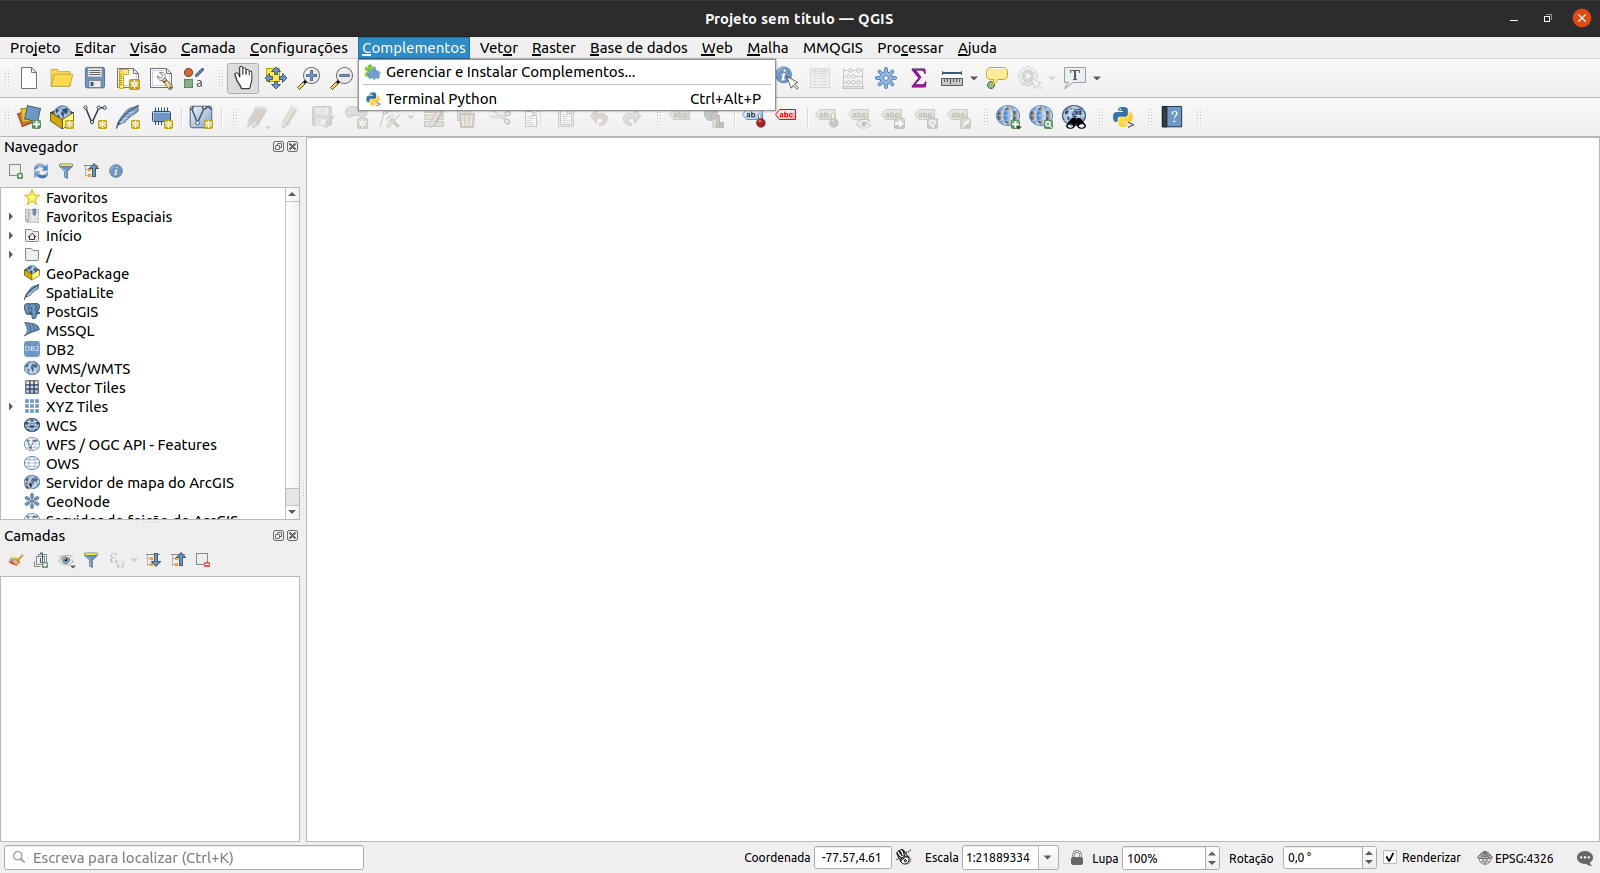
\includegraphics{_bookdown_files/_main_files/figure-html/media/modulo1/plugins-menu.png}
\caption{Menu Gerenciar e Instalar Complementos}
\end{figure}

Figura 1.5. Acessando a caixa de diálogo Gerenciar e instalar complementos

\textbf{Diálogo Gerenciar e Instalar Complementos}

A caixa de diálogo Gerenciar e instalar complementos se conecta ao repositório de complementos oficiais do QGIS (ou qualquer repositório que você indicar na guia Configurações) para buscar complementos disponíveis para sua versão do QGIS. Possui cinco (5) abas:

\begin{itemize}
\tightlist
\item
  \textbf{Aba Tudo} - mostra TODOS os complementos disponíveis para sua versão QGIS, incluindo aqueles que já estão instalados em sua máquina
\item
  \textbf{Aba Instalados} - mostra apenas os complementos instalados em sua máquina
\item
  \textbf{Aba não instalado} - mostra os complementos que não estão instalados em sua máquina
\item
  \textbf{Aba Instalar a partir do do ZIP} - permite que você instale complementos de um arquivo ZIP
\item
  \textbf{Aba Opções} - oferece opções sobre quando verificar se há atualizações de complementos, incluir ou não complementos experimentais e obsoletos ou adicionar / alterar o repositório para buscar complementos
\end{itemize}

Se o complemento que você está procurando está marcado como experimental ou obsoleto, você precisa marcar \textbf{Mostrar complementos experimentais} e \textbf{Mostrar complementos obsoletos} na guia Opções.

A \textbf{Barra de Pesquisa} permite que você pesquise complementos encontrados no(s) repositório(s) de complementos aos quais você está conectado.

\begin{figure}
\centering
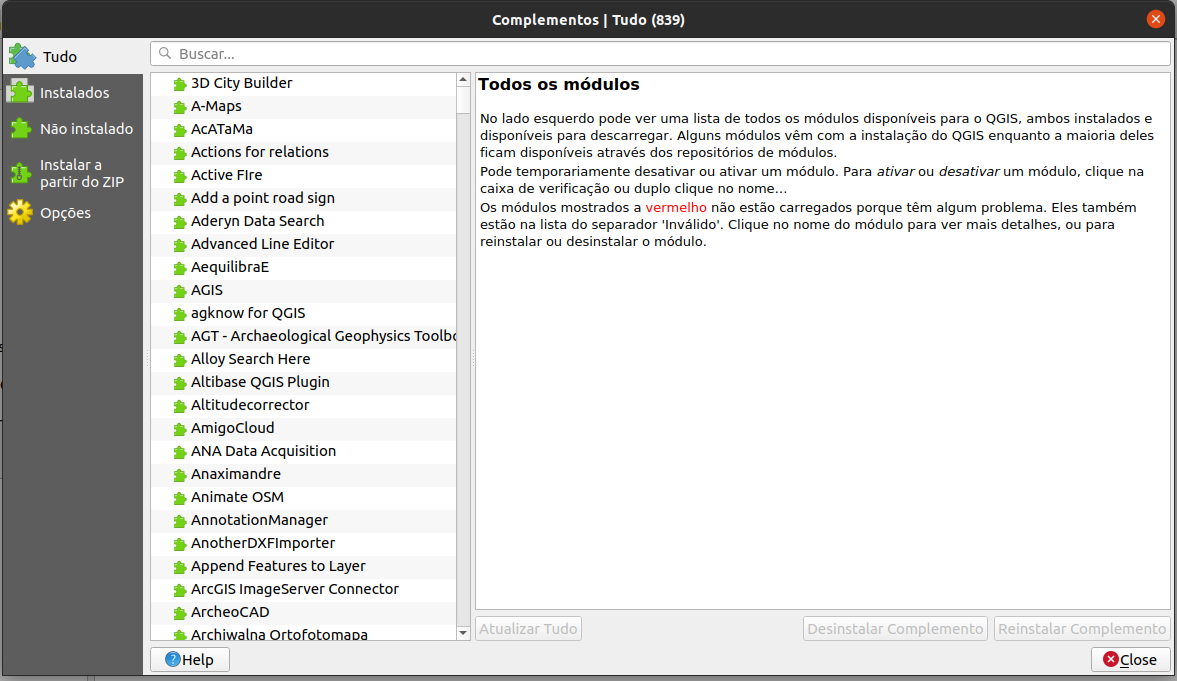
\includegraphics{_bookdown_files/_main_files/figure-html/media/modulo1/manage-and-install-plugins-dialog.png}
\caption{Caixa de diálogo Gerenciar e instalar complementos}
\end{figure}

Figura 1.6. A caixa de diálogo Gerenciar e instalar complementos

\hypertarget{tutorial-exercuxedcio-2-instalando-um-complemento-qgis}{%
\subsubsection{\texorpdfstring{\textbf{Tutorial / Exercício 2: Instalando um complemento QGIS}}{Tutorial / Exercício 2: Instalando um complemento QGIS}}\label{tutorial-exercuxedcio-2-instalando-um-complemento-qgis}}

\begin{enumerate}
\def\labelenumi{\arabic{enumi}.}
\tightlist
\item
  Abra a caixa de diálogo \textbf{Gerenciar e instalar complementos} em \textbf{Complementos ‣ Gerenciar e instalar complementos} na barra de menus. Isso abrirá a caixa de diálogo Gerenciar e instalar complementos.
\end{enumerate}

\begin{figure}
\centering
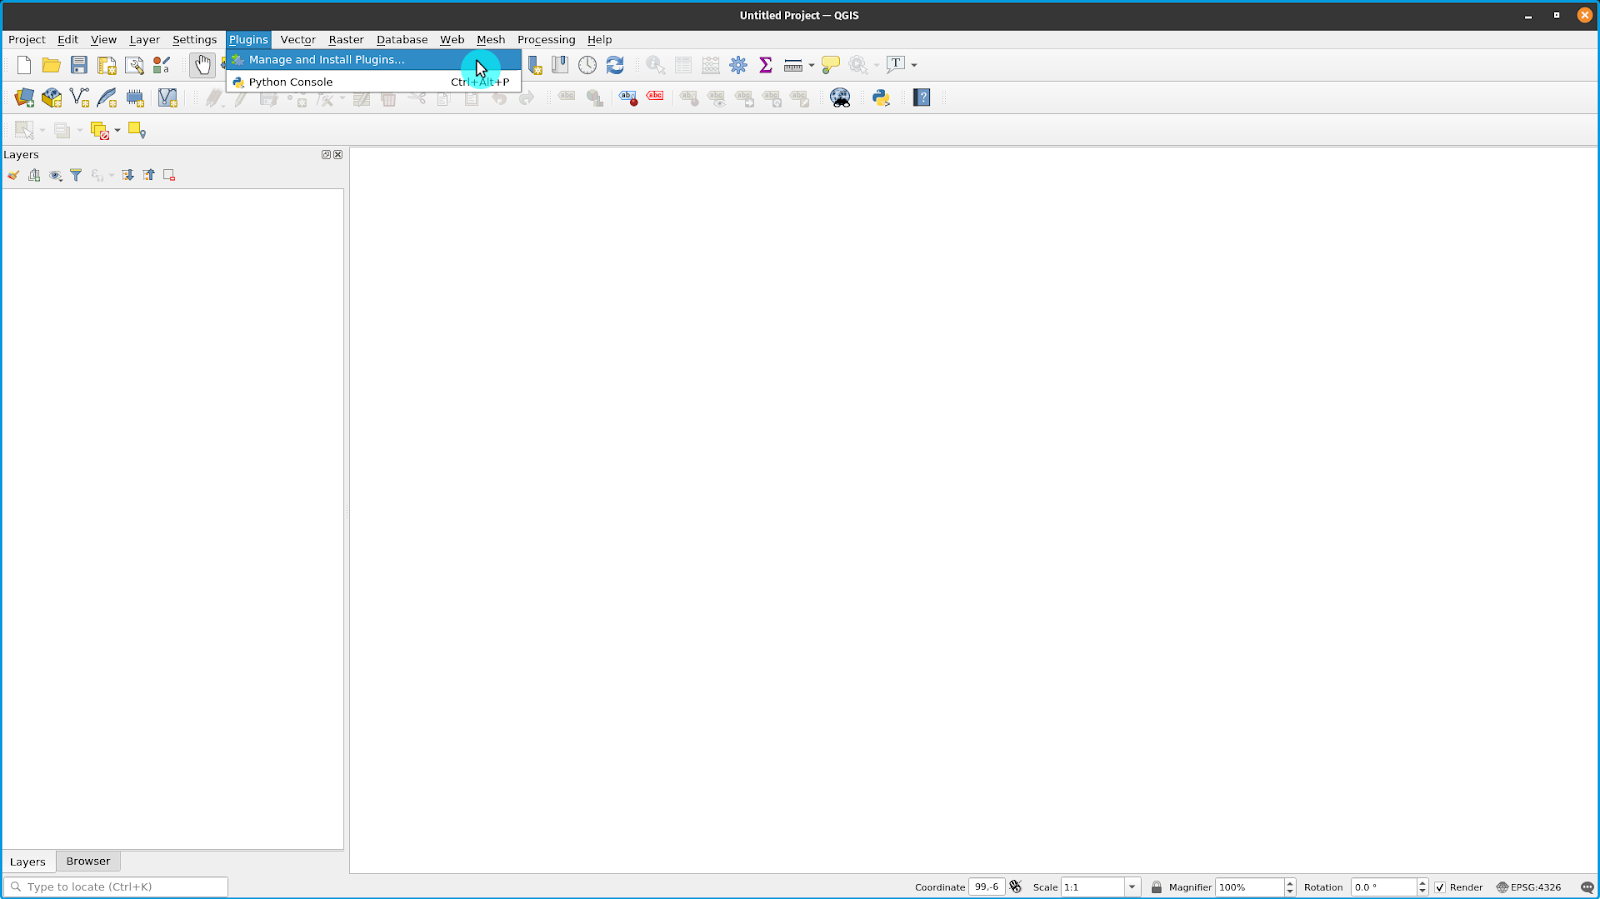
\includegraphics{_bookdown_files/_main_files/figure-html/media/modulo1/plugins-menu-2.png}
\caption{Abrir caixa de diálogo Gerenciar e instalar complementos}
\end{figure}

\begin{figure}
\centering
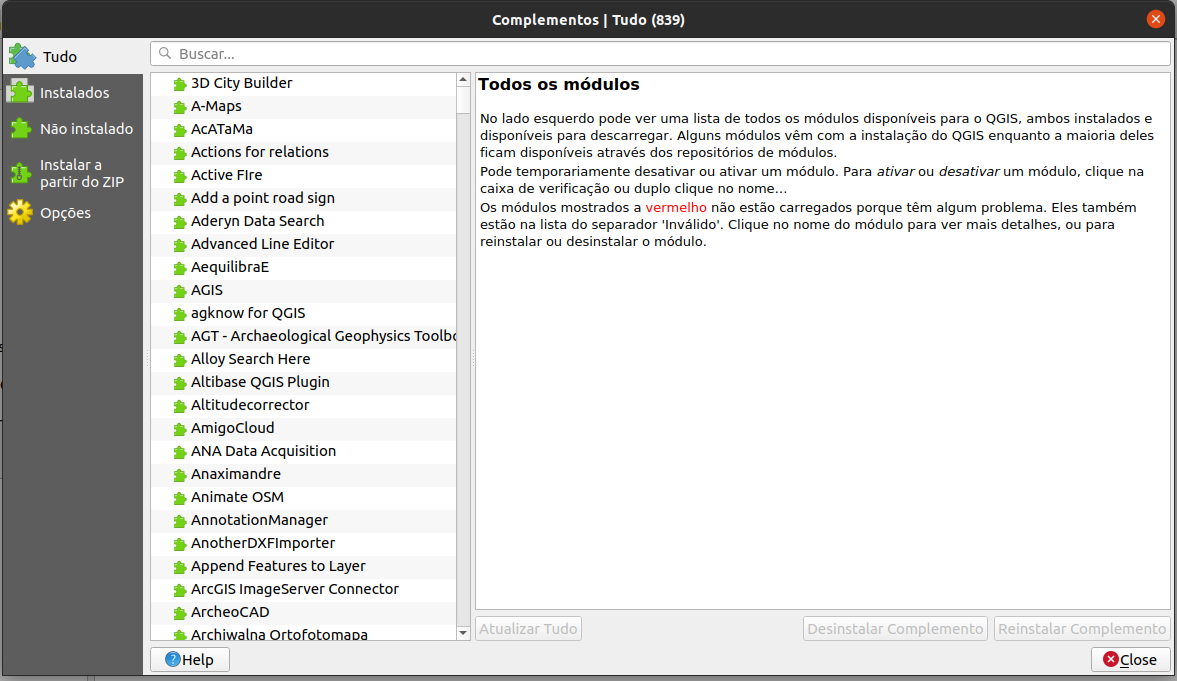
\includegraphics{_bookdown_files/_main_files/figure-html/media/modulo1/manage-and-install-plugins-dialog.png}
\caption{Caixa de diálogo Gerenciar e instalar complementos}
\end{figure}

\begin{enumerate}
\def\labelenumi{\arabic{enumi}.}
\setcounter{enumi}{1}
\tightlist
\item
  Instale os complementos a seguir procurando por eles na guia \textbf{Todos} e clicando em \textbf{Instalar complemento} no canto inferior direito da caixa de diálogo Gerenciar e instalar complementos.

  \begin{itemize}
  \tightlist
  \item
    Memory Layer Saver
  \end{itemize}
\end{enumerate}

\begin{figure}
\centering
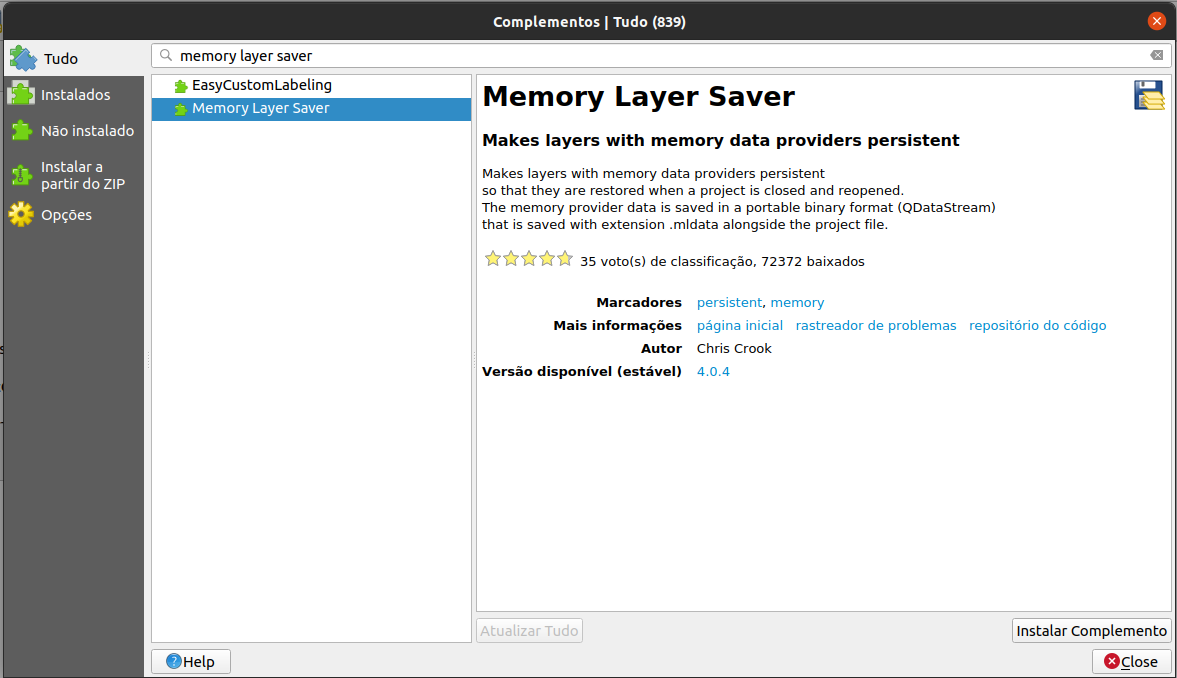
\includegraphics{_bookdown_files/_main_files/figure-html/media/modulo1/memory-layer-saver-plugin.png}
\caption{Instalar o plugin Memory Layer Saver}
\end{figure}

\begin{itemize}
\tightlist
\item
  QuickOSM
\end{itemize}

\begin{figure}
\centering
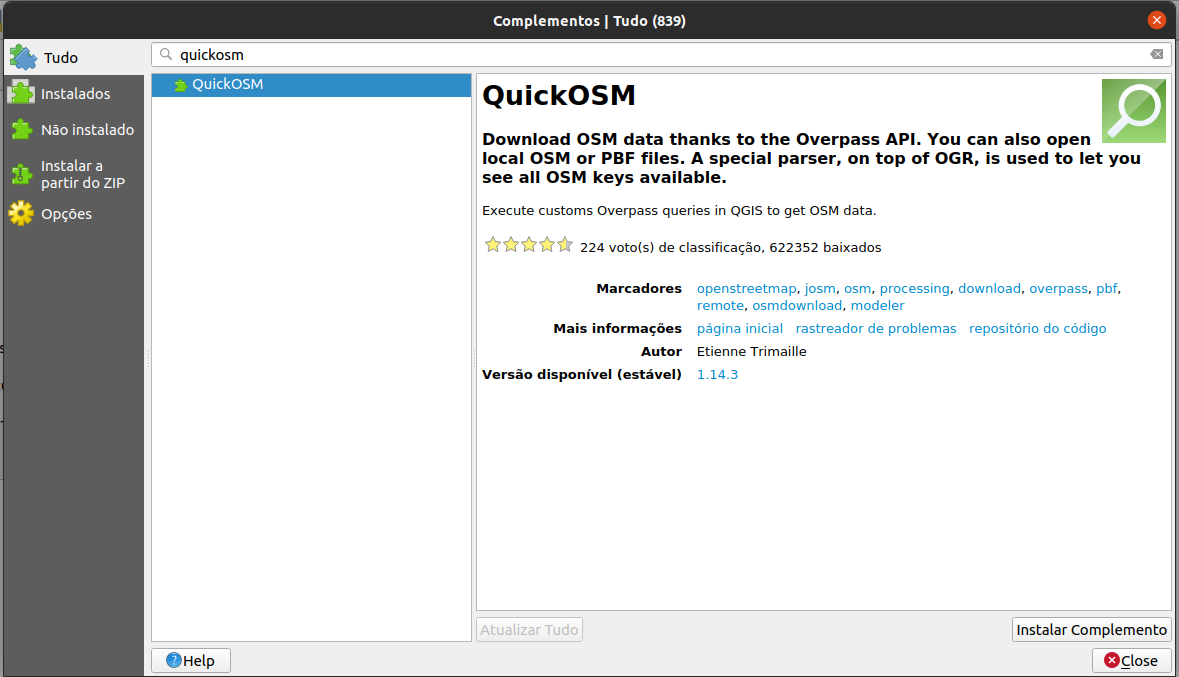
\includegraphics{_bookdown_files/_main_files/figure-html/media/modulo1/quickosm-plugin.png}
\caption{Instalar plugin QuickOSM}
\end{figure}

\begin{enumerate}
\def\labelenumi{\arabic{enumi}.}
\setcounter{enumi}{2}
\tightlist
\item
  Verifique se os complementos foram instalados com sucesso. O plugin Memory Layer Saver deve estar disponível em \textbf{Complementos ‣ Memory Layer Saver} na barra de menus, enquanto o plugin QuickOSM deve estar disponível em \textbf{Vetor ‣ QuickOSM} na barra de menus.
\end{enumerate}

\hypertarget{perguntas-do-questionuxe1rio-3}{%
\subsubsection{\texorpdfstring{\textbf{Perguntas do questionário}}{Perguntas do questionário}}\label{perguntas-do-questionuxe1rio-3}}

\begin{enumerate}
\def\labelenumi{\arabic{enumi}.}
\tightlist
\item
  Verdadeiro ou falso

  \begin{enumerate}
  \def\labelenumii{\arabic{enumii}.}
  \tightlist
  \item
    Você pode remover ou desinstalar os complementos do Core - \textbf{\emph{Falso}}
  \item
    Você pode adicionar complementos que não são encontrados no repositório oficial de complementos do QGIS - \textbf{\emph{Verdadeiro}}
  \end{enumerate}
\end{enumerate}

\hypertarget{tuxedtulo-da-fase-3-configurauxe7uxf5es-qgis}{%
\subsection{Título da Fase 3: Configurações QGIS}\label{tuxedtulo-da-fase-3-configurauxe7uxf5es-qgis}}

\textbf{Configurações do sistema e do projeto}

As configurações do QGIS permitem que você edite e gerencie coisas diferentes sobre o QGIS, como perfis de usuário, estilos, sistemas de referência de coordenadas, atalhos de teclado, a interface do usuário, cores padrão, etc. As configurações do sistema podem ser encontradas no menu \textbf{Configurações} e são as configurações padrão usadas pelo QGIS, a menos que sejam substituídas pelas configurações de um projeto. As configurações do projeto podem ser encontradas em \textbf{Projeto ‣ Propriedades} e referem-se às configurações ou propriedades do projeto atual. Esses valores substituem os padrões do sistema.

\begin{figure}
\centering
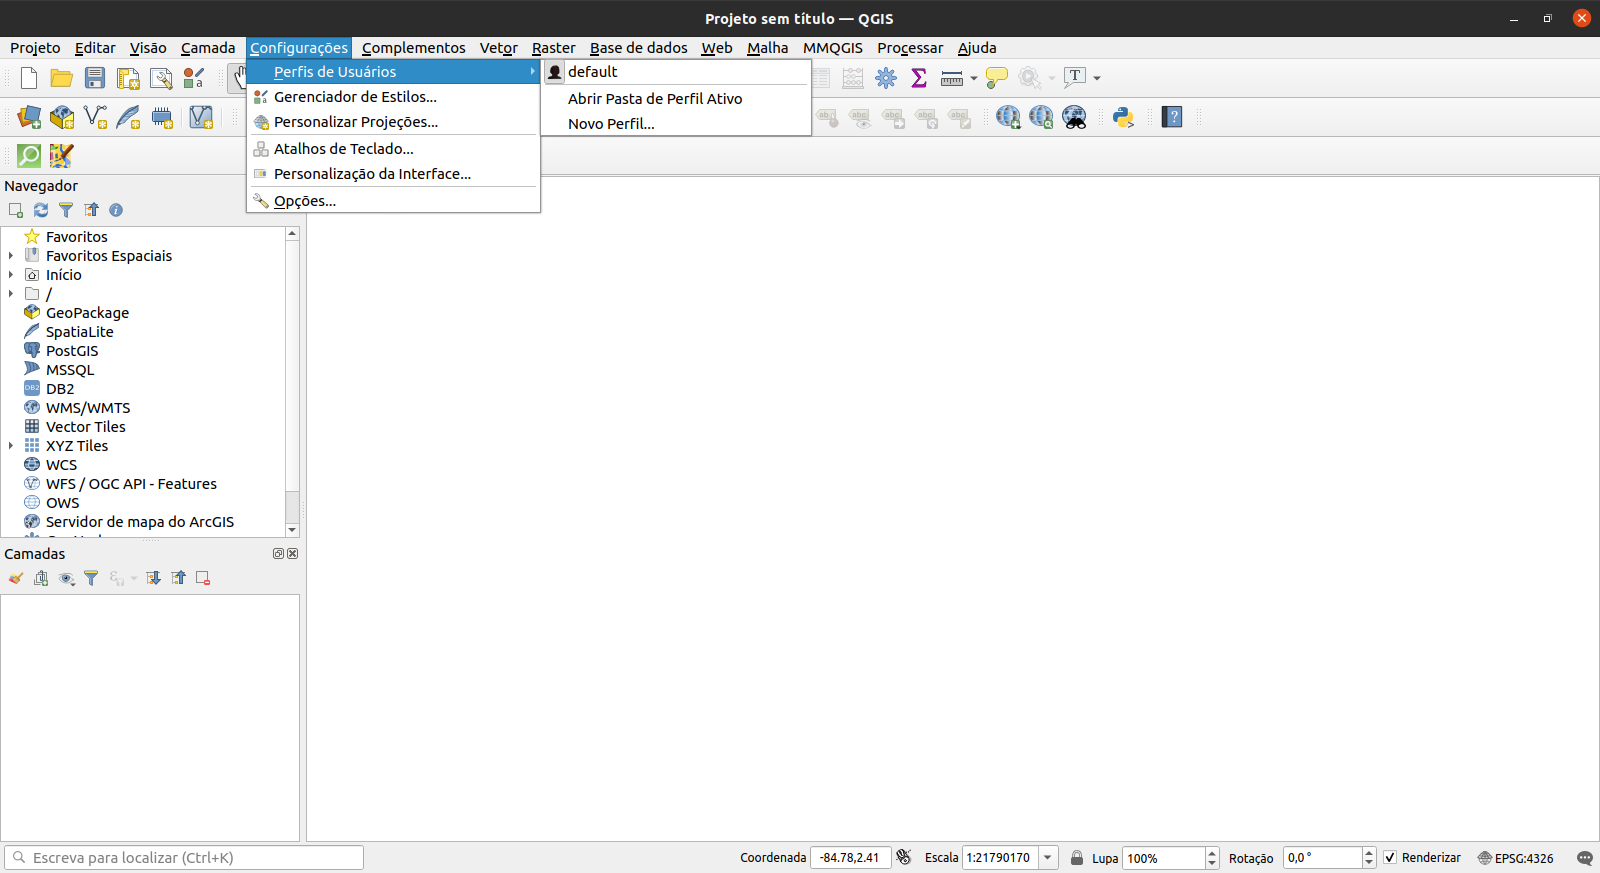
\includegraphics{_bookdown_files/_main_files/figure-html/media/modulo1/settings-1.png}
\caption{As Configurações do Sistema}
\end{figure}

Figura 1.7. As configurações do sistema

\begin{figure}
\centering
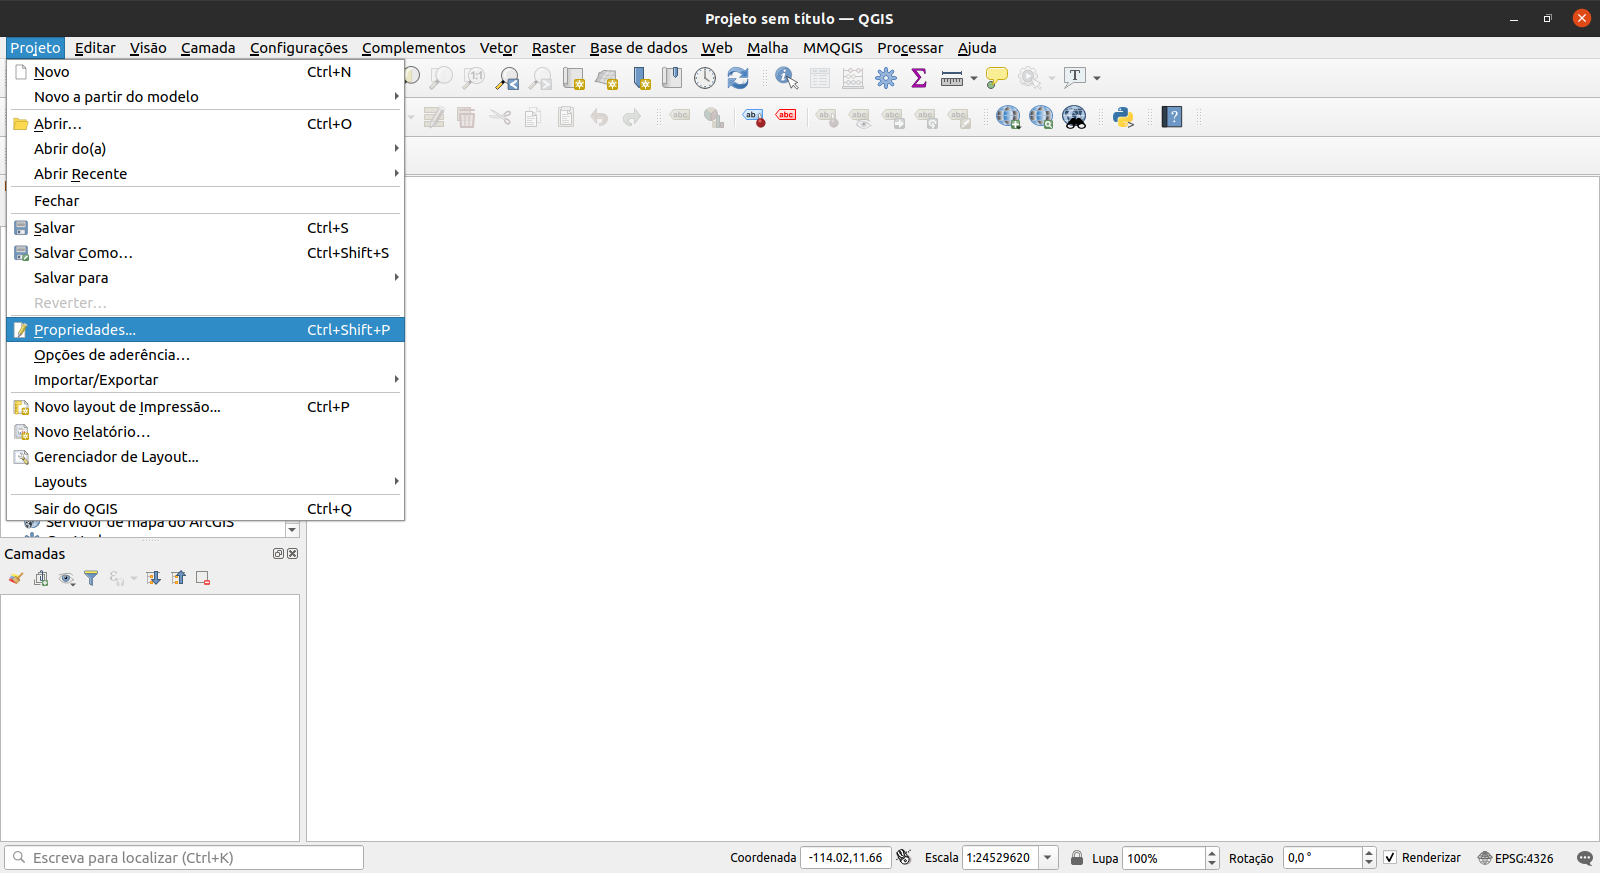
\includegraphics{_bookdown_files/_main_files/figure-html/media/modulo1/settings-2.png}
\caption{Configurações do projeto}
\end{figure}

Figura 1.8. Configurações do projeto

\textbf{Mudando o tema QGIS}

Você pode alterar a aparência do QGIS em \textbf{Configurações ‣ Opções ‣ Aba Geral}.

Você pode escolher entre três temas - padrão (default), Blend of Grey e Night Mapping. Você também pode alterar o tamanho dos ícones, a fonte usada pelo QGIS e outros padrões do sistema.

\begin{figure}
\centering
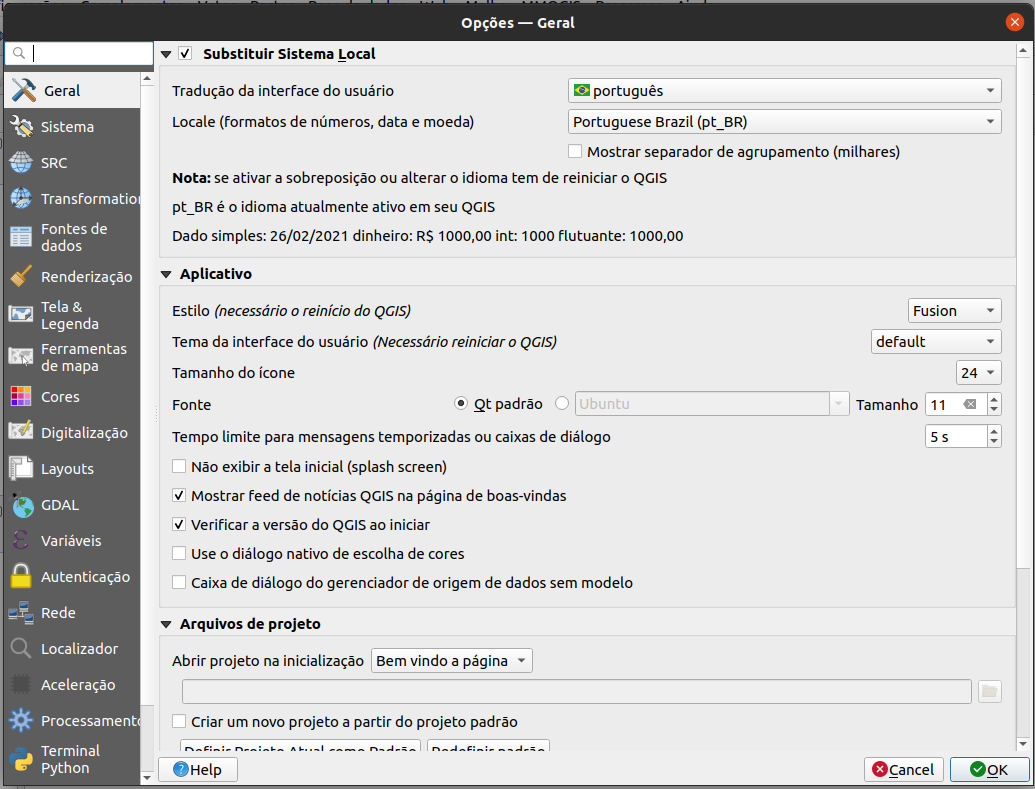
\includegraphics{_bookdown_files/_main_files/figure-html/media/modulo1/change-theme.png}
\caption{Configurações gerais do QGIS}
\end{figure}

Figura 1.9. Configurações gerais do QGIS

Para algumas configurações no QGIS, pode ser necessário reiniciar o aplicativo para que tenham efeito.

\textbf{Perfis de usuário}

QGIS 3.X introduziu o conceito de Perfis de Usuário QGIS.

Um perfil de usuário é uma coleção de configurações para complementos instalados, barras de ferramentas habilitadas, organização da interface do usuário e outras configurações. QGIS vem com um Perfil de Usuário padrão chamado default. Perfis de usuário permitem que o usuário crie configurações diferentes para análises específicas (por exemplo, um perfil de usuário específico para gestão de recursos hídricos, digitalização de dados, cartografia, etc.), projetos particulares ou mesmo clientes.

Perfis de usuário podem ser criados e acessados na barra de menus em: \textbf{Configurações ‣ Perfis de usuário}.

O perfil de usuário ativo é mostrado com {[}Perfil do usuário{]} na barra de título.

\begin{figure}
\centering
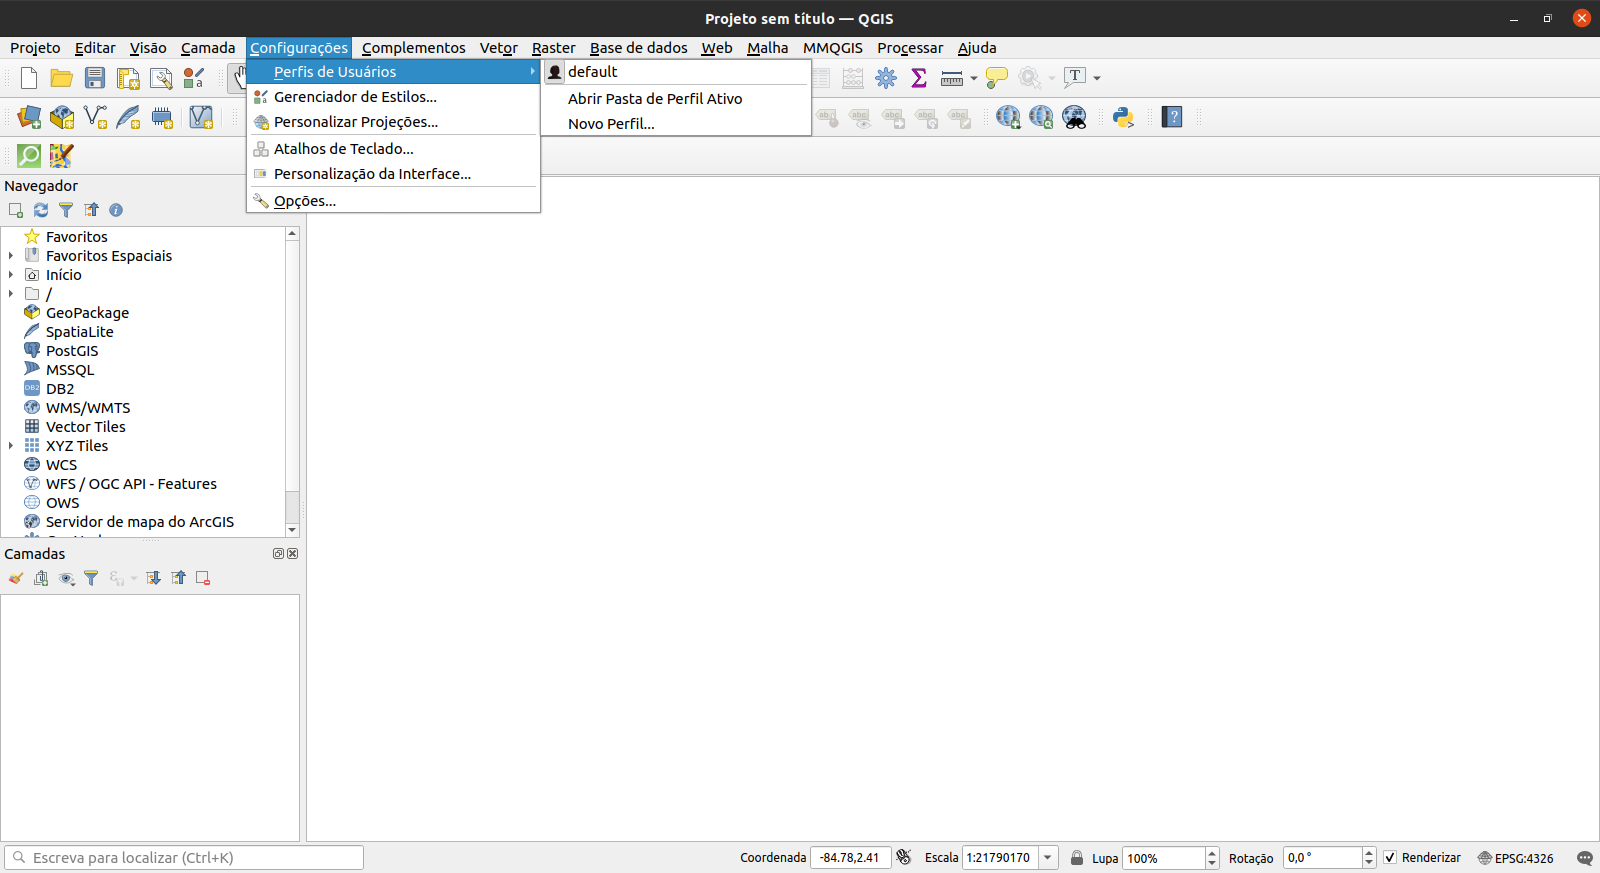
\includegraphics{_bookdown_files/_main_files/figure-html/media/modulo1/user-profiles-1.png}
\caption{Acessando perfis de usuário}
\end{figure}

Figura 1.10. Acessando perfis de usuário

Os perfis de usuário são salvos em um diretório em seu computador que pode ser acessado clicando em \textbf{Configurações ‣ Perfis de usuário ‣ Abrir pasta de perfil ativo}.

\hypertarget{tutorial-exercuxedcio-03-criando-um-perfil-de-usuuxe1rio}{%
\subsubsection{\texorpdfstring{\textbf{Tutorial / Exercício 03: Criando um Perfil de Usuário}}{Tutorial / Exercício 03: Criando um Perfil de Usuário}}\label{tutorial-exercuxedcio-03-criando-um-perfil-de-usuuxe1rio}}

\begin{enumerate}
\def\labelenumi{\arabic{enumi}.}
\tightlist
\item
  Vá para \textbf{Configurações ‣ Perfis de usuário ‣ Novo perfil \ldots{}}
\end{enumerate}

\begin{figure}
\centering
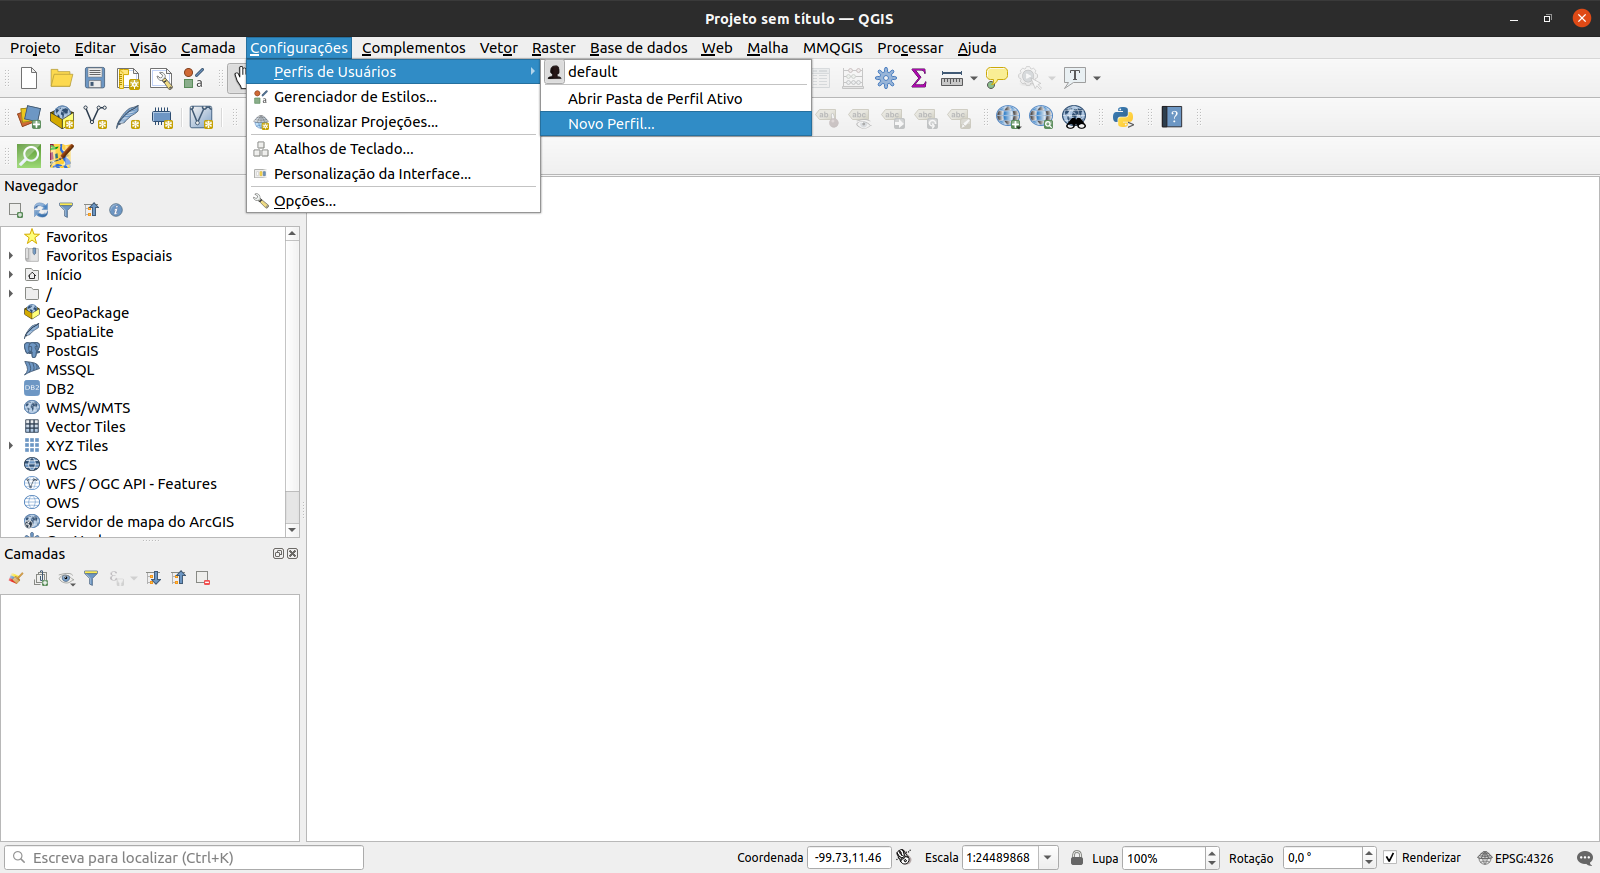
\includegraphics{_bookdown_files/_main_files/figure-html/media/modulo1/user-profiles-2.png}
\caption{alt\_text}
\end{figure}

\begin{enumerate}
\def\labelenumi{\arabic{enumi}.}
\setcounter{enumi}{1}
\tightlist
\item
  Dê um nome ao seu novo perfil de usuário.
\end{enumerate}

\begin{figure}
\centering
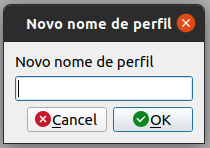
\includegraphics{_bookdown_files/_main_files/figure-html/media/modulo1/user-profiles-3.png}
\caption{alt\_text}
\end{figure}

\begin{enumerate}
\def\labelenumi{\arabic{enumi}.}
\setcounter{enumi}{2}
\item
  Uma nova janela QGIS deve abrir com seu novo perfil de usuário. Observe que o nome do seu perfil é mostrado na barra de título do QGIS.
\item
  Você percebe alguma diferença no novo perfil do usuário? Verifique a interface do usuário, os complementos e as configurações do perfil antigo e do novo perfil que você criou.
\end{enumerate}

\hypertarget{perguntas-do-questionuxe1rio-4}{%
\subsubsection{\texorpdfstring{\textbf{Perguntas do questionário}}{Perguntas do questionário}}\label{perguntas-do-questionuxe1rio-4}}

\begin{enumerate}
\def\labelenumi{\arabic{enumi}.}
\tightlist
\item
  Verdadeiro ou falso

  \begin{enumerate}
  \def\labelenumii{\arabic{enumii}.}
  \tightlist
  \item
    Você só pode ter um perfil de usuário no QGIS. - \textbf{\emph{Falso (você pode ter vários perfis de usuário)}}
  \item
    Você não pode substituir as configurações e propriedades do sistema. - \textbf{\emph{Falso}}
  \end{enumerate}
\end{enumerate}

\hypertarget{tuxedtulo-da-fase-4-adicional-formatos-de-arquivo-do-qgis}{%
\subsection{Título da Fase 4 (adicional): Formatos de arquivo do QGIS}\label{tuxedtulo-da-fase-4-adicional-formatos-de-arquivo-do-qgis}}

\hypertarget{arquivo-de-projeto-qgis-qgs-qgz}{%
\subsubsection{\texorpdfstring{\textbf{Arquivo de projeto QGIS (QGS / QGZ)}}{Arquivo de projeto QGIS (QGS / QGZ)}}\label{arquivo-de-projeto-qgis-qgs-qgz}}

Projetos QGIS estão para QGIS como arquivos .mxd são para ArcMap. Esses arquivos vêm como \textbf{QGS (\emph{.qgs)\textbf{ ou }QGZ (}.qgz)}. A principal diferença entre os dois é que o formato QGZ é um arquivo compactado (zip) contendo um arquivo QGS e um arquivo QGD. O formato QGS é um formato XML para armazenar projetos QGIS. O arquivo QGD é o banco de dados sqlite associado do projeto QGIS que contém dados auxiliares para o projeto. Se não houver dados auxiliares, o arquivo QGD ficará vazio.

Um arquivo de projeto QGIS contém tudo o que é necessário para armazenar um projeto QGIS, incluindo:

\begin{itemize}
\tightlist
\item
  título do projeto
\item
  CRS do projeto
\item
  a árvore de camadas
\item
  configurações de ajuste
\item
  relações
\item
  a extensão da tela do mapa
\item
  modelos de projeto
\item
  legend
\item
  docas mapview (2D e 3D)
\item
  as camadas com links para os conjuntos de dados subjacentes (fontes de dados) e outras propriedades da camada, incluindo extensão, CRS, junções, estilos, renderizador, modo de mesclagem, opacidade e muito mais
\item
  propriedades do projeto
\end{itemize}

Os arquivos do projeto QGIS podem ser salvos em um banco de dados GeoPackage ou PostGIS. Salvar o arquivo do projeto junto com o arquivo de estilo e as camadas correspondentes em um único GeoPackage facilita o compartilhamento de projetos QGIS.

\hypertarget{definiuxe7uxe3o-da-camada-qgis-qlr}{%
\subsubsection{\texorpdfstring{\textbf{Definição da camada QGIS (QLR)}}{Definição da camada QGIS (QLR)}}\label{definiuxe7uxe3o-da-camada-qgis-qlr}}

Um arquivo de definição de camada QGIS (\textbf{QLR}) é um arquivo XML que contém um ponteiro para a fonte de dados da camada, além das informações de estilo QGIS para a camada. Atualmente, um arquivo QLR corresponde a uma única camada apenas.

O caso de uso para este arquivo é simples: ter um único arquivo para abrir uma fonte de dados e trazer todas as informações de estilo relacionadas. Os arquivos QLR também permitem definir a fonte de dados subjacente em um arquivo fácil de abrir.

Um exemplo de uso de QLR é para abrir uma camada de um banco de dados PostGIS. Em vez de se conectar ao banco de dados, encontrar a camada e aplicar um filtro, você pode apenas abrir um arquivo .qlr que aponta para a camada PostGIS correta com seu estilo e filtro correspondentes.

\hypertarget{arquivo-de-estilo-qgis-qml}{%
\subsubsection{\texorpdfstring{\textbf{Arquivo de estilo QGIS (QML)}}{Arquivo de estilo QGIS (QML)}}\label{arquivo-de-estilo-qgis-qml}}

\textbf{QML} é um formato XML para armazenar estilos de camadas. Um arquivo QML (.qml) contém todas as informações que dizem ao QGIS como renderizar geometrias de feições que incluem definições de símbolos, tamanhos e rotações, rótulos, opacidade, modo de mesclagem e muito mais.

Um arquivo .qml deve ter o mesmo nome da fonte de dados a que ele corresponde. Quando ele for encontrado no mesmo diretório ou pasta da fonte de dados, carregar a fonte de dados também carregará automaticamente seu estilo, conforme definido no arquivo .qml.

Por exemplo, se você tiver um GeoJSON chamado \texttt{regioes.geojson} e um arquivo QML chamado \texttt{regioes.qml}, carregar as \texttt{regioes.geojson} no QGIS aplicará os estilos definidos em \texttt{regioes.qml} na camada carregada.

Ao usar GeoPackages (.gpkg), um arquivo .qml muitas vezes não é necessário, pois você pode salvar o estilo de uma camada diretamente no geopacote.

\hypertarget{se-vocuxea-quiser-ir-mais-longe-1}{%
\subsection{Se você quiser ir mais longe:}\label{se-vocuxea-quiser-ir-mais-longe-1}}

Você pode tentar criar seu próprio plugin QGIS. Se não houver um complemento que faça o que você deseja, você pode criar um você mesmo.

O \textbf{Plugin Builder} é um plugin que cria um modelo que pode servir como ponto de partida para o desenvolvimento do plugin QGIS para que você não precise criar um desde o início. Você pode instalá-lo na caixa de diálogo Gerenciar e instalar complementos.

Claro, você sempre pode criar um plugin do zero. Se você estiver interessado em criar seu próprio plugin, pode verificar a documentação oficial do QGIS (\url{https://documentation.qgis.org/}). Para complementos Python, é uma boa ideia verificar o PyQGIS Developer Cookbook (\href{https://docs.qgis.org/3.16/en/docs/pyqgis_developer_cookbook\%20/}{https://docs.qgis.org/3.16/en/docs/pyqgis\_developer\_cookbook/}).

Para obter mais informações, consulte: \href{https://bnhr.xyz/2018/10/08/qgis-plugins-3.0.\%20html}{https://bnhr.xyz/2018/10/08/qgis-plugins-3.0.html}

\hypertarget{para-praticar-suas-novas-habilidades-tente-1}{%
\subsection{Para praticar suas novas habilidades, tente \ldots{}}\label{para-praticar-suas-novas-habilidades-tente-1}}

\begin{itemize}
\tightlist
\item
  Altere o tema e a aparência da interface do usuário QGIS de acordo com sua preferência.
\item
  Instale outros complementos QGIS.
\item
  Altere outras configurações do QGIS.

  \begin{itemize}
  \tightlist
  \item
    Crie um sistema de referência de coordenadas personalizado
  \item
    Adicione uma tela inicial personalizada (\href{https://bnhr.xyz/2020/09/05/custom-splash\%20-screen-qgis.html}{https://bnhr.xyz/2020/09/05/custom-splash-screen-qgis.html})
  \end{itemize}
\end{itemize}

\hypertarget{dicas-1}{%
\subsection{Dicas}\label{dicas-1}}

N/D

\hypertarget{camadas-no-qgis}{%
\chapter{Camadas no QGIS}\label{camadas-no-qgis}}

\textbf{Autor}: Ben Hur

\hypertarget{introduuxe7uxe3o-pedaguxf3gica-2}{%
\section{Introdução Pedagógica}\label{introduuxe7uxe3o-pedaguxf3gica-2}}

Este módulo irá ensinar-lhe os conceitos básicos das camadas no QGIS e como carregá-las. No final deste módulo, os alunos devem estar familiarizados com:

\begin{itemize}
\tightlist
\item
  as diferentes fontes de dados e formatos de arquivo que podem ser carregados no QGIS
\item
  as diferentes maneiras que os dados podem ser carregados no QGIS
\item
  alguns formatos de arquivo de dados comuns
\end{itemize}

Eles também devem ser capazes de:

\begin{itemize}
\tightlist
\item
  carregar camadas (vetores e rasters) usando o painel do navegador e o gerenciador de fonte de dados
\item
  conectar o QGIS a serviços remotos
\item
  trabalhar com camadas temporárias e virtuais
\item
  instalar alguns plug-ins que carregarão outros conjuntos de dados no QGIS
\item
  mostrar propriedades da camada, como metadados informações
\item
  salvar e exportar camadas
\end{itemize}

\hypertarget{ferramentas-e-recursos-necessuxe1rios-2}{%
\section{Ferramentas e recursos necessários}\label{ferramentas-e-recursos-necessuxe1rios-2}}

As ferramentas e recursos necessários para este módulo são:

\begin{itemize}
\tightlist
\item
  computador
\item
  conexão à Internet
\item
  QGIS 3.16 instalado no computador (\href{https://qgis.org/en/site/forusers/download.html}{https://qgis.org/en/site/forusers /download.html})
\end{itemize}

\hypertarget{pruxe9-requisitos-2}{%
\section{Pré-requisitos}\label{pruxe9-requisitos-2}}

\begin{itemize}
\tightlist
\item
  conhecimento básico de operação de um computador
\item
  familiaridade com formatos de dados espaciais e a interface QGIS (conclusão dos Módulos 0 e 1)
\end{itemize}

\hypertarget{recursos-adicionais-2}{%
\section{Recursos adicionais}\label{recursos-adicionais-2}}

\begin{itemize}
\tightlist
\item
  QGIS User Guide - \url{https://docs.qgis.org/3.16/en/docs/user_manual/}
\item
  Manual de treinamento QGIS - \url{https://docs.qgis.org/3.16/en/docs/training_manual/index.html}
\item
  Basemaps no QGIS - \url{https://bnhr.xyz/2018/10/07/basemaps-in-qgis.html}
\item
  Conectando o QGIS ao Serviços remotos - {[}\url{https://bnhr.xyz/2018/10/12/connecting-qgis-to-remote-services.html}{]} (\url{https://bnhr.xyz/2018/10/12/connecting-qgis-to} -remote-services.html)
\item
  Spreadsheet Layers Plugin - \href{https://bnhr.xyz/2018/\%2027/07\%20/\%20plugin-fridays-spreadsheet-layers-plugin.html}{https://bnhr.xyz/2018/07/27/plugin-fridays-spreadsheet-layers-plugin.html}
\end{itemize}

\hypertarget{introduuxe7uxe3o-temuxe1tica-2}{%
\section{Introdução temática}\label{introduuxe7uxe3o-temuxe1tica-2}}

\begin{figure}
\centering
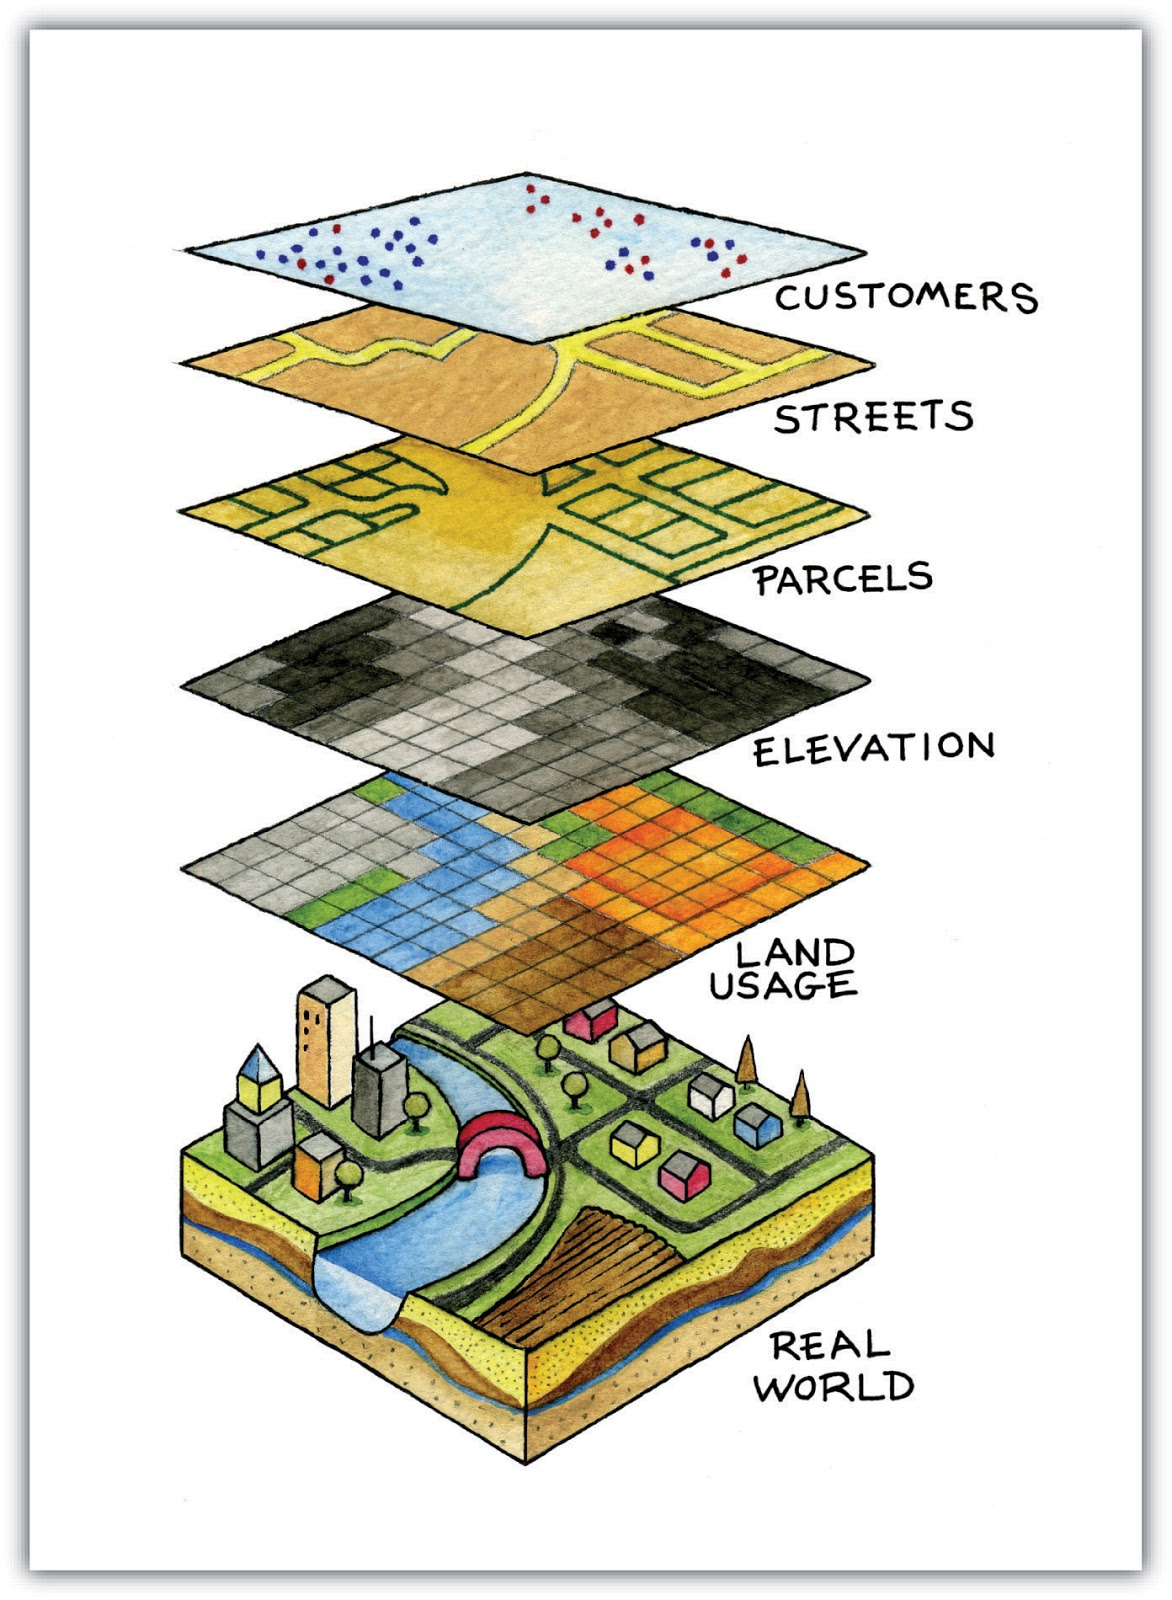
\includegraphics{_bookdown_files/_main_files/figure-html/media/modulo2/spatial-layers.jpg}
\caption{Análise de múltiplas camadas em GIS}
\end{figure}

Figura 2.1. Uma sobreposição de mapa contendo diferentes camadas e tipos de dados (\href{https://saylordotorg.\%20github.io/text_essentials-of-geographic-information-systems/s11-02-multiple-layer-analysis.html}{https://saylordotorg.github.io/text\_essentials-of-geographic-information-systems/s11-02-multiple-layer-analysis.html})

Aprendemos nos módulos anteriores que modelos de dados espaciais, como vetores e rasters, são modelos de objetos do mundo real e fenômenos e, embora seja perfeitamente normal ter uma única camada que modele uma única coisa (por exemplo, elevação, temperatura, localização de residências, zoneamento, etc.), na prática, se quisermos realizar análises úteis ou criar um modelo que reflita o mundo real melhor, então, precisaríamos usar vários dados e camadas juntos. Sobrepor vários mapas temáticos da mesma área, colocando-os uns sobre os outros, é uma das técnicas de análise geográfica mais antigas e comuns.

\hypertarget{detalhamento-dos-conceitos-1}{%
\section{Detalhamento dos conceitos}\label{detalhamento-dos-conceitos-1}}

A imagem acima nos dá um exemplo simples e concreto disso. Imagine que você é um consultor GIS encarregado de encontrar a melhor localização para uma nova escola. Para fazer isso, você precisaria reunir as informações relevantes que o ajudariam a decidir. Isso pode incluir informações sobre as ruas da cidade, lotes de terreno, localização e distribuição de possíveis estudantes, a topografia da área, uso do solo, etc.

Esses conjuntos de dados podem vir em diferentes tipos e formatos. Alguns podem ser arquivos vetoriais, enquanto outros podem ser raster. Alguns podem estar no mesmo sistema de referência de coordenadas, enquanto outros podem estar em sistemas de referência de coordenadas diferentes. Alguns podem ser arquivos locais encontrados em seu computador, enquanto outros só podem ser carregados pela Internet. Por causa das muitas possibilidades do tipo de dados que você precisaria para sua análise espacial, um bom GIS deve ser capaz de manipular e gerenciar uma variedade de fontes de dados.

\hypertarget{conteuxfado-principal-2}{%
\section{Conteúdo principal}\label{conteuxfado-principal-2}}

\hypertarget{tuxedtulo-da-fase-1-tipos-de-dados-formatos-de-arquivo-o-painel-do-navegador-e-o-painel-de-camadas}{%
\subsection{Título da fase 1: Tipos de dados, formatos de arquivo, o painel do navegador e o painel de camadas}\label{tuxedtulo-da-fase-1-tipos-de-dados-formatos-de-arquivo-o-painel-do-navegador-e-o-painel-de-camadas}}

\hypertarget{tipos-de-dados-e-formatos-de-arquivo-comuns}{%
\subsubsection{\texorpdfstring{\textbf{Tipos de dados e formatos de arquivo comuns}}{Tipos de dados e formatos de arquivo comuns}}\label{tipos-de-dados-e-formatos-de-arquivo-comuns}}

Além dos modelos de dados espaciais (rasters e vetores) discutidos no primeiro módulo, a familiaridade com formatos de arquivo geoespaciais e seus prós e contras também é importante para qualquer pessoa que faça análise espacial.

A maioria das pessoas que são novas em GIS geralmente são apresentadas aos dados espaciais por meio de shapefiles. A maioria das pessoas nunca supera esse formato e usa shapefiles para todos os tipos e formas de dados vetoriais. Isso é semelhante a como uma marca específica como a Coca Cola começa a ser usada como o termo geral para refrigerantes. Isso não é necessariamente errado, mas é lamentável, pois os shapefiles são apenas um dos muitos tipos de formato de dados vetoriais. Na verdade, há muitos outros formatos de vetor como geopackage, geojson, topojson e flatgeobuf. O formato do shapefile, embora onipresente, tem algumas limitações significativas, como:

\begin{itemize}
\tightlist
\item
  Não é apenas um arquivo único. Na verdade, um shapefile consiste em vários arquivos, 3 dos quais são obrigatórios: .shp, .shx, .dbf. Todos os outros arquivos são chamados de arquivos secundários (sidecar).
\item
  Tem um limite de tamanho de 2 GB para cada arquivo individual.
\item
  Os nomes dos campos são limitados a 10 caracteres.
\item
  Colunas de atributos são limitadas a 255 colunas.
\item
  Não há suporte para alguns tipos de dados, como tempo.
\item
  Não armazena explicitamente topologia.
\end{itemize}

Outros formatos de dados, como GeoPackage, GeoJSON, TopoJSON e flatgeobuf, corrigem essas limitações dos shapefiles. Na verdade, QGIS e GRASS GIS mudaram para GeoPackage como o formato de arquivo vetorial padrão ao importar ou exportar camadas e, embora GeoPackage também tenha algumas limitações, é um formato completamente aberto e permite que a comunidade ajude a moldar o futuro do formato.

Então, se não shapefiles, o que você deve usar?

Não há nada de errado em usar shapefiles, especialmente se for adequado ao seu caso de uso. Se você não precisa de um conjunto de dados que vai além de 2 GB; se não houver problema em ter um limite de 10 caracteres para os nomes dos campos; ou se você estiver trabalhando com um pequeno número de arquivos localmente, um shapefile é totalmente adequado.

No entanto, se você deseja empacotar seu projeto QGIS junto com todas as camadas (vetores, rasters), estilos e modelos; ou você deseja compartilhar vários tipos de camadas e dados espaciais em um único arquivo, vale a pena dar uma olhada em um GeoPackage. GeoPackages e GeoJSONs também são compatíveis com a web e podem ser usados diretamente por bibliotecas de mapeamento da web, como Mapbox e Leaflet.

Você pode ler mais no link abaixo: \href{https://bnhr.xyz/2018/12/12/i-choose\%20-geopackage.html}{https://bnhr.xyz/2018/12/12/i-choose-geopackage.html}

Enquanto isso, qualquer formato que pode ser representado como uma grade de pixels ou células pode ser lido pelo QGIS como dados raster. Isso inclui formatos de imagem como PNG (.png) e JPEG (.jpg). É importante notar que embora todos os formatos de arquivo de imagem possam ser lidos como rasters, nem todos são georreferenciados ou contêm informações geoespaciais que nos permitem localizá-los corretamente na Terra. Para instâncias como essa, podemos usar o que é conhecido como um arquivo mundial (ou world) (\url{https://en.wikipedia.org/wiki/World_file}). Um arquivo world é um arquivo de dados de texto simples separado, cujo nome é o mesmo do arquivo raster ao qual pertence e cuja extensão de arquivo tem a letra w adicionada ao final. Por exemplo, o arquivo world para \textbf{world.png} será nomeado \textbf{world.pngw} ou \textbf{world.pgw}.

Alguns formatos de arquivo de imagem contêm georreferenciamento e informações explícitas e não precisam de um arquivo word. Alguns exemplos são GeoTIFFs (.tif ou tiff) e formato de arquivo ERDAS Imagine (.img).

Para obter mais informações sobre formatos de arquivo, você também pode acessar: \href{https://saylordotorg.\%20github.io/text_essentials-of-geographic-information-systems/s09-03-file-formats.html}{https://saylordotorg.github.io/text\_essentials-of-geographic-information-systems/s09-03-file-formats.html} Os

Dados geoespaciais também podem vir no formato de bancos de dados geoespaciais. Eles podem ser bancos de dados de nível empresarial, como o Postgres, gratuito e de código aberto, com extensão PostGIS (\url{https://postgis.net/}) ou ArcSDE, proprietário da ESRI. Existem também bancos de dados geográficos de arquivos que podem armazenar diferentes tipos de dados (por exemplo, vetores e rasters) dentro deles. Alguns exemplos são o OGC GeoPackage, gratuito e aberto (.gpkg) (\url{https://www.geopackage.org/}) e o formato patenteado File Geodatabase da ESRI (.gdb).

\hypertarget{tipos-de-fontes-de-dados}{%
\subsubsection{\texorpdfstring{\textbf{Tipos de fontes de dados}}{Tipos de fontes de dados}}\label{tipos-de-fontes-de-dados}}

Um dos recursos mais poderosos do QGIS é sua capacidade de conectar, carregar e usar diferentes dados espaciais e não espaciais de uma variedade de fontes. O QGIS pode abrir:

\begin{itemize}
\tightlist
\item
  arquivos raster e vetoriais
\item
  bancos de dados locais
\item
  arquivos e bancos de dados na Internet por meio de seu identificador de recurso uniforme (URI) ou localizador de recurso uniforme (URL),
\item
  serviços da web (serviços da web OSGeo e serviços da web ArcGIS), tile services e portais de dados como GeoNode
\item
  e muitos mais\ldots{}
\end{itemize}

O QGIS também pode conectar e carregar dados de serviços como dados SRTM da NASA, imagens do planeta, SentinelHub, Google Earth Engine e OpenStreetMap através de plug-ins.

Isso torna o QGIS um componente integral para qualquer infraestrutura ou fluxo de trabalho de dados espaciais.

\hypertarget{carregando-camadas-no-qgis}{%
\subsubsection{\texorpdfstring{\textbf{Carregando camadas no QGIS}}{Carregando camadas no QGIS}}\label{carregando-camadas-no-qgis}}

Existem várias maneiras de carregar camadas no QGIS. Estes incluem:

\begin{enumerate}
\def\labelenumi{\arabic{enumi}.}
\tightlist
\item
  \textbf{Arraste e solte} a camada na Tela do Mapa QGIS ou no Painel de Camadas. Esta pode ser a maneira mais fácil de carregar uma camada no QGIS, mas não é a abordagem recomendada, pois há várias coisas que podem dar errado ao usar esta abordagem, como ao carregar dados tabulares não espaciais, por exemplo CSVs.
\item
  Usando o \textbf{Painel do navegador}.
\item
  Usando o \textbf{Gerenciador de fonte de dados}.
\item
  Usando a \textbf{barra de ferramentas do Gerenciador de fonte de dados} e a \textbf{barra de ferramentas Gerenciar camadas}.
\end{enumerate}

** NOTA: ** \emph{Ao carregar camadas, as cores padrão de suas camadas podem ser diferentes das cores padrão mostradas neste módulo.}

\hypertarget{o-painel-do-navegador}{%
\subsubsection{\texorpdfstring{\textbf{O painel do navegador}}{O painel do navegador}}\label{o-painel-do-navegador}}

O \textbf{Painel do navegador} exibe uma árvore de arquivos que mostra os arquivos e pastas do seu computador, bem como as conexões com bancos de dados e servidores web. Por padrão, ele é encaixado no lado esquerdo da interface do usuário QGIS junto com o Painel de Camadas.

O painel do navegador expõe muitas funcionalidades para conectar, carregar e mostrar informações sobre camadas. Você também pode criar conexões para diretórios favoritos e marcadores espaciais no painel do navegador.

Para saber mais sobre o painel do navegador, acesse: \href{https://docs.qgis.org/3.16/en\%20/docs/user_manual/introduction/browser.html}{https://docs.qgis.org/3.16/en/docs/user\_manual/introduction/browser.html}

\hypertarget{exercuxedcio-01.1-o-painel-do-navegador}{%
\subsubsection{\texorpdfstring{\textbf{Exercício 01.1: O painel do navegador}}{Exercício 01.1: O painel do navegador}}\label{exercuxedcio-01.1-o-painel-do-navegador}}

\begin{enumerate}
\def\labelenumi{\arabic{enumi}.}
\tightlist
\item
  Abra o QGIS.
\item
  Verifique o painel do navegador (Figura 2.2). Se você não conseguir encontrar o painel do navegador, pode torná-lo visível em \textbf{Exibir ‣ Painéis ‣ Painel do navegador} na barra de menus.
\end{enumerate}

\begin{figure}
\centering
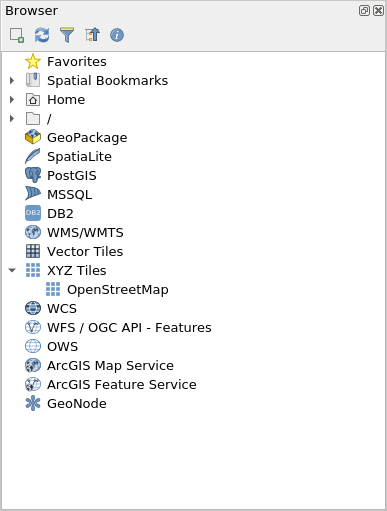
\includegraphics{_bookdown_files/_main_files/figure-html/media/modulo2/qgis-browser-1.png}
\caption{O painel do navegador QGIS}
\end{figure}

Figura 2.2. O painel do navegador

\begin{enumerate}
\def\labelenumi{\arabic{enumi}.}
\setcounter{enumi}{2}
\tightlist
\item
  Observe como os drives e pastas podem ser expandidas para mostrar as subpastas dentro delas.
\item
  Localize a pasta \textbf{Módulo 2 - Camadas no QGIS} (Figura 2.3) na árvore de arquivos (observe onde você salvou ou baixou o arquivo). Você deve ser capaz de ver os dados necessários para esta pasta de trabalho. No meu exemplo à direita, vinculei a pasta mencionada a um dos meus Favoritos para acessá-la facilmente no painel do navegador. Você pode adicionar um diretório favorito ao Painel do navegador clicando com o botão direito em Favoritos e adicionando o diretório.
\item
  Verifique os arquivos dentro da pasta (Figura 2.3). Existem vários deles. A partir da própria árvore de arquivos, já podemos ter uma ideia dos arquivos e camadas que podemos carregar no QGIS. Os ícones à esquerda dos nomes indicam se os dados são um vetor 
\includegraphics{_bookdown_files/_main_files/figure-html/media/modulo2/symbol-vector.png}, um raster 
\includegraphics{_bookdown_files/_main_files/figure-html/media/modulo2/symbol-raster.png}, um banco de dados 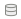
\includegraphics{_bookdown_files/_main_files/figure-html/media/modulo2/symbol-db.png" Símbolo do banco de dados"} ou dados tabulares simples 
\includegraphics{_bookdown_files/_main_files/figure-html/media/modulo2/symbol-table.png}.
\end{enumerate}

\begin{figure}
\centering
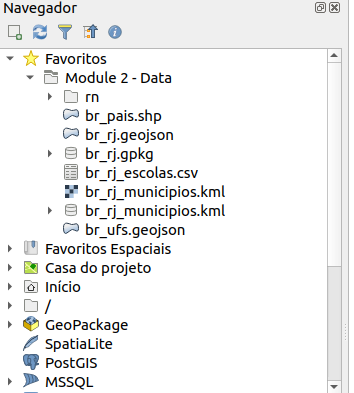
\includegraphics{_bookdown_files/_main_files/figure-html/media/modulo2/qgis-browser-2.png}
\caption{Arquivos do módulo 2 no painel do navegador}
\end{figure}

Figura 2.3. Os arquivos do módulo no painel do navegador

\begin{enumerate}
\def\labelenumi{\arabic{enumi}.}
\setcounter{enumi}{5}
\item
  Existem 5 arquivos na pasta de dados:

  \begin{enumerate}
  \def\labelenumii{\arabic{enumii}.}
  \tightlist
  \item
    um GeoPackage (br\_rj.gpkg) que contém um arquivo vetorial (br\_rj\_hospitais) e raster (br\_rj\_srtm\_dem);
  \item
    um GeoJSON (br\_ufs.geojson);
  \item
    um arquivo kml (br\_rj\_municipios.kml);
  \item
    um arquivo de forma (br\_pais.shp); e
  \item
    um arquivo de valores separados por vírgula (CSV) (br\_rj\_escolas.csv).
  \end{enumerate}
\item
  Clique com o botão direito em br\_pais.shp e clique em Propriedades da camada (Figura 2.4). Isso abre a janela de propriedades da camada (Figura 2.5). Observe as informações fornecidas na janela. Qual é a geometria da camada? Qual CRS é usado? Quantos recursos existem na camada?
\end{enumerate}

\begin{figure}
\centering
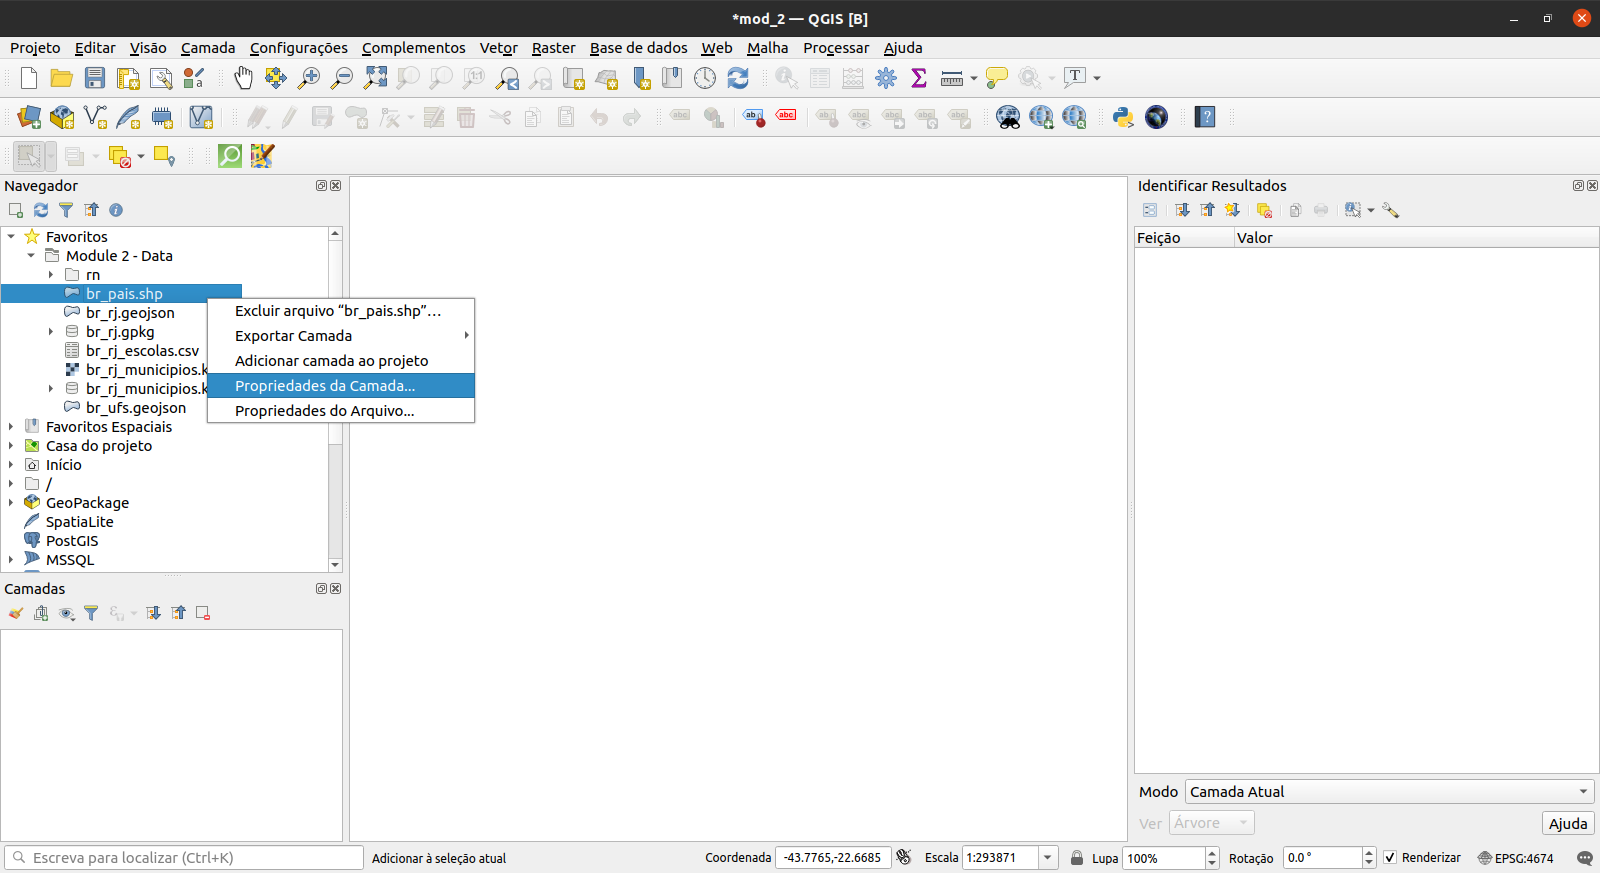
\includegraphics{_bookdown_files/_main_files/figure-html/media/modulo2/qgis-browser-3.png}
\caption{Verificando as propriedades da camada}
\end{figure}

Figura 2.4 Verificando as propriedades da camada

\begin{figure}
\centering
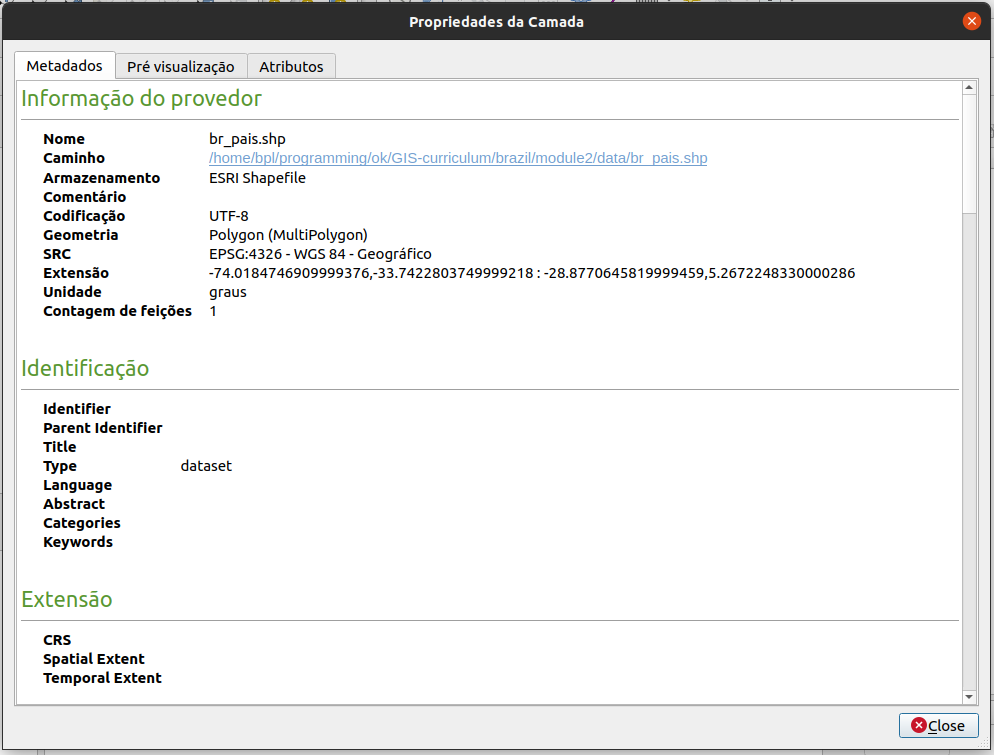
\includegraphics{_bookdown_files/_main_files/figure-html/media/modulo2/qgis-browser-layer-properties.png}
\caption{Propriedades da camada no painel do navegador}
\end{figure}

Figura 2.5. Propriedades da camada no painel do navegador

\begin{enumerate}
\def\labelenumi{\arabic{enumi}.}
\setcounter{enumi}{7}
\item
  Além de fornecer metadados nas camadas, você também pode visualizar a geometria e os atributos da camada na janela de propriedades da camada.
\item
  Você pode carregar uma camada do painel do navegador:

  \begin{enumerate}
  \def\labelenumii{\arabic{enumii}.}
  \tightlist
  \item
    \textbf{clicando duas vezes na camada}
  \item
    \textbf{clicando com o botão direito na camada ‣ Adicionar camada ao projeto}
  \item
    \textbf{arrastando a camada para a área do mapa}
  \end{enumerate}
\item
  Tente carregar as camadas \textbf{br\_pais}, \textbf{br\_ufs} e \textbf{br\_rj\_municipios} usando qualquer um dos métodos acima.
\end{enumerate}

\begin{figure}
\centering
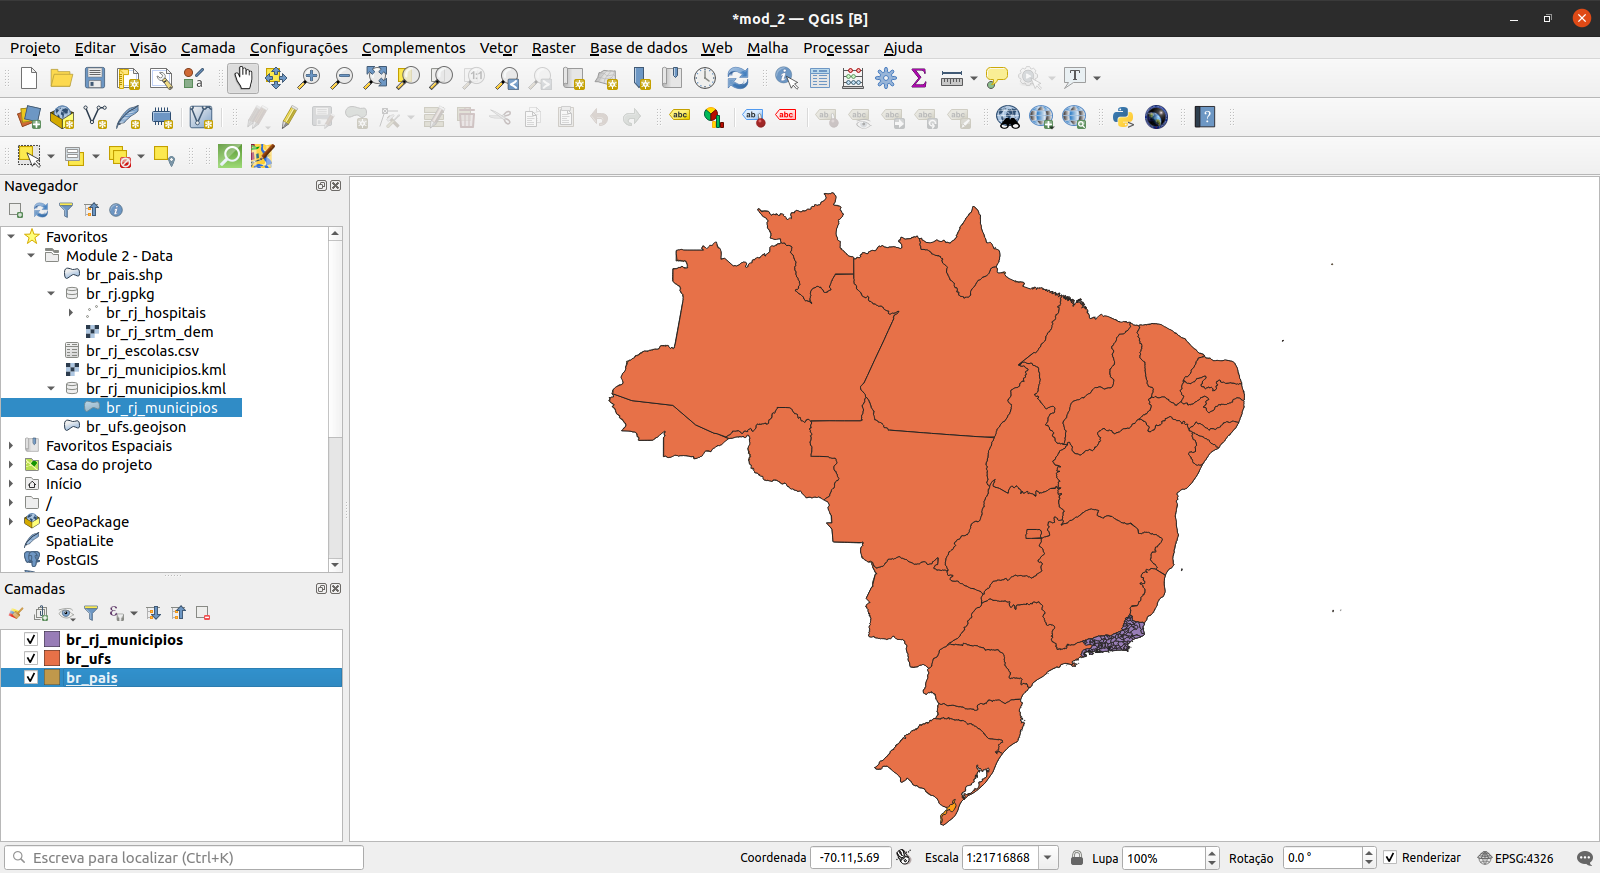
\includegraphics{_bookdown_files/_main_files/figure-html/media/modulo2/vector-layers-loaded-1.png}
\caption{As camadas vetoriais carregadas no QGIS}
\end{figure}

Figura 2.6. As camadas vetoriais carregadas no QGIS

\hypertarget{o-painel-de-camadas}{%
\subsubsection{\texorpdfstring{\textbf{O painel de camadas}}{O painel de camadas}}\label{o-painel-de-camadas}}

O painel de camadas lista todas as camadas atuais no projeto. Ele ajuda a gerenciar sua visibilidade e ordem e pode ser usado para mostrar as propriedades da camada. O painel de camadas pode ser ativado em \textbf{Exibir ‣ Painéis ‣ Painel de camadas} ou usando o atalho \textbf{CTRL + 1}. Ele também é chamado de legenda do mapa. Se você carregou todos os vetores do exercício anterior, seu painel de camadas deve aparecer como abaixo:

\begin{figure}
\centering
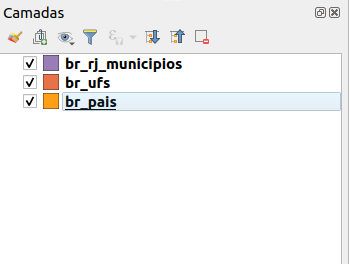
\includegraphics{_bookdown_files/_main_files/figure-html/media/modulo2/layers-panel-1.png}
\caption{Painel de camadas}
\end{figure}

Figura 2.7. O painel de camadas

A visibilidade de uma camada pode ser controlada marcando ou desmarcando a caixa à esquerda do nome da camada. Ao arrastar as camadas para cima ou para baixo no painel Camadas, sua ordem pode ser alterada. Semelhante ao software de manipulação de imagem como GIMP ou Photoshop, as camadas listadas perto do topo são desenhadas sobre as camadas listadas abaixo. Portanto, se duas camadas mostrarem a mesma área, a camada mais alta no painel camadas será desenhada no topo da camada inferior e pode ocultar a camada inferior na tela do mapa. É importante notar esse ponto porque pode haver casos em que pensamos que uma camada não aparece no QGIS quando na realidade está sendo coberta ou escondida por uma camada em cima dela.

\textbf{NOTA:} A ordem Z das camadas no Painel de camadas pode ser substituída pelo \textbf{Painel de ordem das camadas}.

O painel de camadas também permite ao usuário renomear e remover camadas, filtrar a visibilidade da camada, criar e gerenciar grupos de camadas e visualizações de mapas.

A tabela de atributos de uma camada vetorial também pode ser aberta no painel Camadas \textbf{clicando com o botão direito do mouse na camada ‣ Abrir tabela de atributos}.

Para saber mais sobre o painel de camadas, acesse: \href{https://docs.qgis.org\%20/3.16/en/docs/user_manual/introduction/general_tools.html\#layers-panel}{https://docs.qgis.org/3.16/en/docs/user\_manual/introduction/general\_tools.html\#layers-panel}

\hypertarget{propriedades-da-camada}{%
\subsubsection{\texorpdfstring{\textbf{Propriedades da camada}}{Propriedades da camada}}\label{propriedades-da-camada}}

Clicar com o botão direito em uma camada no painel Camadas e selecionar Propriedades da camada abrirá a caixa de diálogo Propriedades da camada.

\begin{figure}
\centering
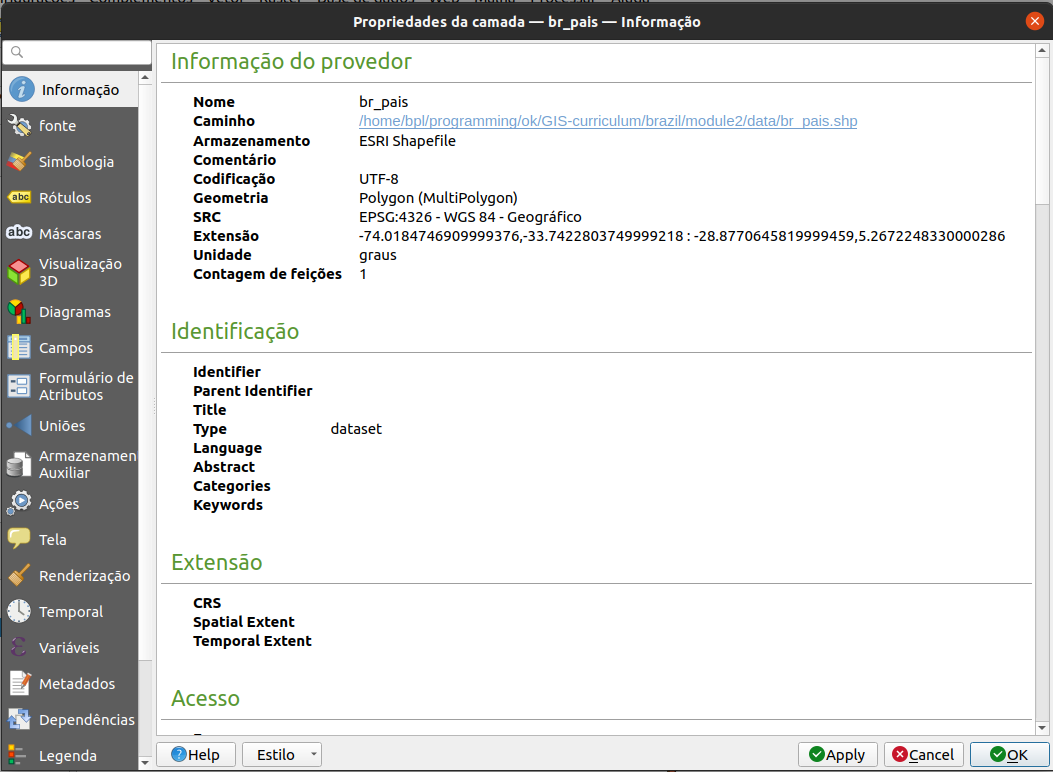
\includegraphics{_bookdown_files/_main_files/figure-html/media/modulo2/layer-properties.png}
\caption{A caixa de diálogo Propriedades da camada}
\end{figure}

Figura 2.8. A caixa de diálogo Propriedades da camada

Existem várias guias na caixa de diálogo Propriedades da camada que permitem ao usuário ver informações e até mesmo editar / modificar propriedades relacionadas à camada.

A guia Informações mostra uma representação somente leitura de informações resumidas e metadados da camada atual, incluindo:

\begin{itemize}
\tightlist
\item
  o provedor de dados
\item
  metadados
\item
  geometria ou informações de campo
\end{itemize}

A guia Fonte mostra as configurações gerais para uma camada vetorial.

Abas como Simbologia, Rótulos, Máscaras e Visualização 3D permitem que o usuário modifique a simbologia e o estilo da camada.

Outras guias permitem que os usuários realizem junções com a Camada (Junção), obtenham informações sobre os campos de atributos (Campos), adicionem Formulários personalizados para adicionar novos dados (Formulários de Atributo) e muito mais.

Outra guia que vale a pena mencionar é a guia Metadados, que fornece ao usuário a capacidade de criar e editar um relatório de metadados na camada. Isso inclui informações sobre:

\begin{itemize}
\tightlist
\item
  Identificação de dados: atribuição básica do conjunto de dados (dado pai, identificador, título, resumo, idioma \ldots);
\item
  Categorias às quais os dados pertencem, como categorias ISO e personalizadas;
\item
  Palavras-chave para recuperar os dados e conceitos associados seguindo um vocabulário padrão;
\item
  Acesso ao conjunto de dados (licenças, direitos, taxas e restrições);
\item
  Extensão do conjunto de dados, seja espacial (CRS, extensão do mapa, altitudes) ou temporal;
\item
  Contato do(s) proprietário(s) do conjunto de dados;
\item
  Links para recursos auxiliares e informações relacionadas; e
\item
  História do conjunto de dados.
\end{itemize}

Um resumo das informações preenchidas é fornecido na guia Validação e ajuda a identificar possíveis problemas relacionados ao formulário de metadados. Atualmente, os metadados são salvos no arquivo de projeto, mas também podem ser salvos em um arquivo .qmd separado ao lado das camadas baseadas em arquivo ou em um banco de dados .sqlite local para camadas remotas.

Para saber mais sobre as propriedades da camada vetorial, acesse: \href{https://docs.qgis.org/3.16/en\%20/docs/user_manual/working_with_vector/vector_properties.html}{https://docs.qgis.org/3.16/en/docs/user\_manual/working\_with\_vector/vector\_properties.html}

Para saber mais sobre as propriedades da camada raster, vá para: \href{https:\%20//docs.qgis.org/3.16/en/docs/user_manual/working_with_raster/raster_properties.html}{https://docs.qgis.org/3.16/en/docs/user\_manual/working\_with\_raster/raster\_properties.html}

\hypertarget{metadados-geoespaciais}{%
\subsubsection{\texorpdfstring{\textbf{Metadados geoespaciais}}{Metadados geoespaciais}}\label{metadados-geoespaciais}}

Metadados são simplesmente dados sobre os dados. Eles responde, o ``quem, o que, quando, onde e como'' dos dados e vem em todas as formas e tamanhos. Para fins de GIS, geralmente estamos preocupados com metadados geoespaciais. Os metadados geoespaciais são descritos pelo US Federal Geographic Data Committee (FGDC) como:

\emph{``um arquivo de informações, geralmente apresentado como um documento XML, que captura as características básicas de um recurso de dados ou informações. Representa quem, o quê, quando, onde, por que e como do recurso. Metadados geoespaciais comumente documentam dados digitais geográficos, como arquivos de Sistema de Informação Geográfica (GIS), bancos de dados geoespaciais e imagens da Terra, mas também podem ser usados para documentar recursos geoespaciais, incluindo catálogos de dados, aplicativos de mapeamento, modelos de dados e sites relacionados. Os registros de metadados incluem os principais elementos do catálogo da biblioteca, como Título, Resumo e Dados de Publicação; elementos geográficos, como extensão geográfica e informações de projeção; e elementos de banco de dados, como Definições de Rótulo de Atributo e Valores de Domínio de Atributo.''}

A importância dos metadados é que eles não apenas promovem a transparência, mas também facilitam o compartilhamento de dados e informações. É por isso que é importante sempre adicionar metadados aos nossos conjuntos de dados. Ao adicionar metadados, é igualmente importante seguir padrões - regras e práticas amplamente promovidas, aceitas e seguidas - para que os metadados que criamos sejam interoperáveis. Um desses padrões é a ISO 19115: 2014 ``Informação Geográfica - Metadados'' da ISO / TC 211 ({[}\url{https://www.iso.org/obp/ui/\#iso:std:iso:19115:-1:ed-1:v1:en}{]} (\url{https://www.iso.org/obp/ui/\#iso:std:iso:19115:-1:ed-1:v1:en}))

\hypertarget{exercuxedcio-01.2-adicionando-metadados}{%
\subsubsection{\texorpdfstring{\textbf{Exercício 01.2: Adicionando metadados}}{Exercício 01.2: Adicionando metadados}}\label{exercuxedcio-01.2-adicionando-metadados}}

\begin{enumerate}
\def\labelenumi{\arabic{enumi}.}
\tightlist
\item
  Abra as Propriedades da camada da camada br\_pais.
\item
  Verifique as informações mostradas na guia Informações e observe as informações mostradas. Está completo? Podemos adicionar mais informações?
\end{enumerate}

\begin{figure}
\centering
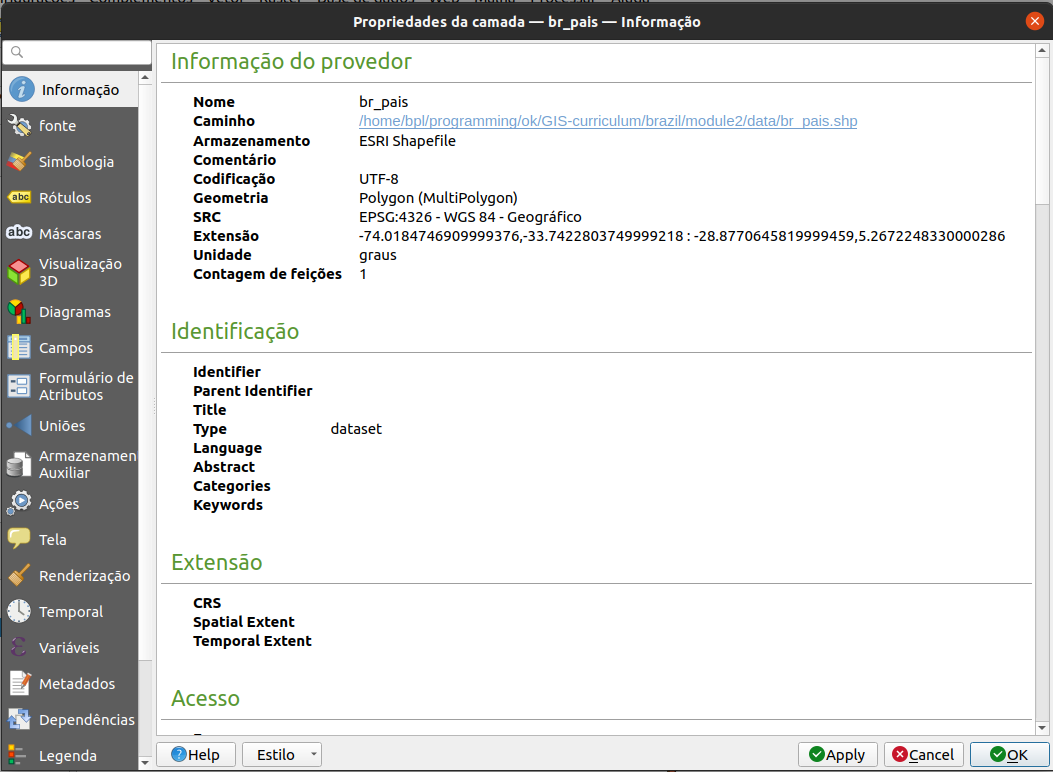
\includegraphics{_bookdown_files/_main_files/figure-html/media/modulo2/metadata-1.png}
\caption{Propriedades de informações da camada br\_pais}
\end{figure}

Figura 2.9. Propriedades de informações da camada br\_pais

\begin{enumerate}
\def\labelenumi{\arabic{enumi}.}
\setcounter{enumi}{2}
\tightlist
\item
  Vá para a guia Metadados e tente adicionar mais informações sobre a camada, como extensão, categoria de dados, licença, etc. Clique em OK quando terminar.
\end{enumerate}

\begin{figure}
\centering
\includegraphics{_bookdown_files/_main_files/figure-html/media/modulo2/metadata-2.png}
\caption{Editando alguns metadados}
\end{figure}

Figura 2.10. Editando alguns metadados

\begin{enumerate}
\def\labelenumi{\arabic{enumi}.}
\setcounter{enumi}{3}
\tightlist
\item
  Vá para a guia Informações novamente e veja se algo mudou.
\end{enumerate}

\begin{figure}
\centering
\includegraphics{_bookdown_files/_main_files/figure-html/media/modulo2/metadata-3.png}
\caption{A guia Informações após a edição de alguns metadados}
\end{figure}

Figura 2.11. A guia Informações depois de editar alguns metadados

\hypertarget{perguntas-do-questionuxe1rio-5}{%
\subsubsection{Perguntas do questionário}\label{perguntas-do-questionuxe1rio-5}}

\begin{enumerate}
\def\labelenumi{\arabic{enumi}.}
\item
  Verdadeiro ou falso:

  \begin{enumerate}
  \def\labelenumii{\arabic{enumii}.}
  \tightlist
  \item
    Todos os arquivos vetoriais são shapefiles. - *** Falso (um shapefile é um formato de arquivo de um arquivo vetorial. Outros formatos de arquivo de dados vetoriais incluem geopackage, geojson e flatgeobuf) ***
  \item
    Quando renderizado no mapa, uma camada que é superior no painel de camadas sempre cobrirá ou aparecerá no topo de uma camada que está abaixo no painel de camadas. - *** Falso (quando ativado, a ordem no painel de ordem de camadas substituirá a ordem no painel de camadas) ***
  \item
    Você pode verificar as informações de metadados sobre uma camada no painel Camadas e no painel do navegador. - *** Verdadeiro ***
  \end{enumerate}
\end{enumerate}

\hypertarget{tuxedtulo-da-fase-2-o-gerenciador-de-fonte-de-dados-e-conexuxe3o-com-serviuxe7os-remotos}{%
\subsection{Título da fase 2: O gerenciador de fonte de dados e conexão com serviços remotos}\label{tuxedtulo-da-fase-2-o-gerenciador-de-fonte-de-dados-e-conexuxe3o-com-serviuxe7os-remotos}}

\hypertarget{o-gerenciador-de-fonte-de-dados}{%
\subsubsection{\texorpdfstring{\textbf{O Gerenciador de fonte de dados}}{O Gerenciador de fonte de dados}}\label{o-gerenciador-de-fonte-de-dados}}

Se você não quiser usar o painel do navegador para carregar camadas, você sempre pode usar o \textbf{Gerenciador de fonte de dados}.

O \textbf{Gerenciador de fonte de dados} foi introduzido com o lançamento do QGIS 3. É um local único para adicionar e carregar camadas de diferentes fontes de dados no QGIS. Antes de sua introdução, havia janelas separadas para carregar diferentes fontes de dados (ou seja, uma para rasters, outra para vetores, etc.). Ele pode ser acessado via \textbf{Camadas ‣ Gerenciador de fonte de dados} ou \textbf{CTRL + L}.

\begin{figure}
\centering
\includegraphics{_bookdown_files/_main_files/figure-html/media/modulo2/data-source-manager-1.png}
\caption{Gerenciador de fonte de dados}
\end{figure}

Figura 2.12. O Gerenciador de fonte de dados

\hypertarget{exercuxedcio-02.1-o-gerenciador-de-fonte-de-dados}{%
\subsubsection{\texorpdfstring{\textbf{Exercício 02.1: O Gerenciador de fonte de dados}}{Exercício 02.1: O Gerenciador de fonte de dados}}\label{exercuxedcio-02.1-o-gerenciador-de-fonte-de-dados}}

\begin{enumerate}
\def\labelenumi{\arabic{enumi}.}
\item
  Abra o \textbf{Gerenciador de fonte de dados}. Ele contém guias no lado direito que pertencem ao tipo de fonte de dados que você deseja carregar ou conectar. Semelhante ao navegador, você pode carregar e conectar vários tipos de dados do Gerenciador de fonte de dados.
\item
  \textbf{Carregando vetores}

  \begin{enumerate}
  \def\labelenumii{\arabic{enumii}.}
  \item
    Para carregar vetores, vá para a guia Vetor. Podem ser carregados arquivos, arquivos dentro de um diretório, um banco de dados e até mesmo arquivos remotos por meio de um protocolo como HTTP, nuvem, etc.
  \item
    Vamos carregar o arquivo vetorial (br\_rj\_hospitais) encontrado dentro do geopackage br\_rj. Esta camada é uma camada de pontos das localizações dos hospitais na cidade do Rio de Janeiro.

    \begin{enumerate}
    \def\labelenumiii{\arabic{enumiii}.}
    \tightlist
    \item
      Tipo de fonte: Arquivo
    \item
      Fonte: Selecione o geopackage br\_rj usando o botão \includegraphics{media/data-source-manager-search.png}
    \item
      Clique em Adicionar
    \item
      Se houver mais de 1 arquivo vetorial dentro do geopackage, o QGIS pedirá que você selecione quais carregar.
    \end{enumerate}
  \end{enumerate}
\end{enumerate}

\begin{figure}
\centering
\includegraphics{_bookdown_files/_main_files/figure-html/media/modulo2/data-source-manager-vector.png}
\caption{Carregando um vetor dentro de um GeoPackage}
\end{figure}

Figura 2.13. Carregando um vetor dentro de um GeoPackage

\begin{enumerate}
\def\labelenumi{\arabic{enumi}.}
\setcounter{enumi}{2}
\item
  \textbf{Carregando Rasters}

  \begin{enumerate}
  \def\labelenumii{\arabic{enumii}.}
  \item
    Para carregar um raster, vá para a aba Raster. Arquivos e arquivos remotos podem ser carregados por meio de um protocolo como HTTP, nuvem, etc. Há um raster (br\_rj\_srtm\_dem) dentro do geopackage br\_rj. Este raster é um modelo digital de elevação da região da cidade do Rio de Janeiro. Para carregá-lo:

    \begin{enumerate}
    \def\labelenumiii{\arabic{enumiii}.}
    \tightlist
    \item
      Tipo de fonte: Arquivo
    \item
      Fonte: Selecione o geopackage br\_rj usando o botão pesquisar \includegraphics{_bookdown_files/_main_files/figure-html/media/modulo2/data-source-manager-search.png}
    \item
      Clique em Adicionar
    \item
      Se há mais de 1 arquivo raster dentro do geopackage, o QGIS irá pedir para você selecionar quais carregar
    \end{enumerate}
  \end{enumerate}
\end{enumerate}

\begin{figure}
\centering
\includegraphics{_bookdown_files/_main_files/figure-html/media/modulo2/data-source-manager-raster.png}
\caption{Carregando um raster dentro de um GeoPackage}
\end{figure}

Figura 2.14. Carregando um raster dentro de um GeoPackage

\begin{enumerate}
\def\labelenumi{\arabic{enumi}.}
\setcounter{enumi}{3}
\item
  \textbf{Carregando CSV e outros arquivos de texto delimitado}

  \begin{enumerate}
  \def\labelenumii{\arabic{enumii}.}
  \item
    Além de vetores e rasters, outro arquivo comum em GIS são CSVs e planilhas. Felizmente, é relativamente fácil carregar esses arquivos no QGIS.
  \item
    CSVs e outros arquivos de texto delimitados podem ser carregados por meio da guia Texto Delimitado no Gerenciador de Fonte de Dados, adicionando-os do Painel do Navegador e até mesmo arrastando-os para a Tela do Mapa. No entanto, algumas coisas devem ser consideradas se o CSV que você possui contém informações de geometria (por exemplo, localizações de pontos). A regra geral é:

    \begin{enumerate}
    \def\labelenumiii{\arabic{enumiii}.}
    \tightlist
    \item
      Use o Gerenciador de fonte de dados para carregar CSVs, quer eles contenham ou não informações de geometria.
    \item
      Se os CSVs forem carregados por meio do painel do navegador ou arrastando-os, certifique-se de que haja um arquivo CSVT correspondente para preservar os tipos de dados do campo.
    \item
      Se você encontrar problemas ao preservar os tipos de dados para seus textos delimitados (especificamente CSVs), você pode usar o que é chamado de arquivo CSVT. Você pode ler mais sobre como carregar CSVs no QGIS no seguinte link: \href{https:\%20//bnhr.xyz/2018/08/07/specifying-csv-data-types-using-a-csvt-file.html}{https://bnhr.xyz/2018/08/07/specifying-csv-data-types-using-a-csvt-file.html}
    \end{enumerate}
  \item
    CSVs e planilhas podem ser carregados no QGIS com ou sem informações espaciais ou geométricas. Quando carregados com informações espaciais, são tratados como dados vetoriais. Quando são carregados sem, são tratados como dados tabulares normais.
  \item
    Há um arquivo CSV na pasta de dados denominado br\_rj\_escolas.csv que contém as localizações das escolas no Rio de Janeiro. Para carregá-lo:

    \begin{enumerate}
    \def\labelenumiii{\arabic{enumiii}.}
    \item
      Vá para a guia Texto delimitado
    \item
      Nome do arquivo: Selecione o br\_rj\_escolas CSV usando o botão pesquisar \includegraphics{_bookdown_files/_main_files/figure-html/media/modulo2/data-source-manager-search.png}
    \item
      Formato de arquivo: CSV
    \item
      Opções de registro e campos: mantenha o padrão
    \item
      Definição de geometria:

      \begin{itemize}
      \tightlist
      \item
        Coordenadas de ponto
      \item
        Campo X: longitude
      \item
        Campo Y: latitude
      \item
        Geometria CRS: EPSG: 4326 - WGS 84
      \end{itemize}
    \item
      Configurações de camada: Marque Olhar arquivo e Usar índice espacial

      \begin{itemize}
      \tightlist
      \item
        Quando Olhar arquivo é marcado, as atualizações para o CSV local são refletidas automaticamente na camada carregada no QGIS.
      \item
        Usar índice espacial adicione um índice espacial à camada carregada, o que torna o processamento vetorial mais rápido.
      \end{itemize}
    \end{enumerate}
  \end{enumerate}
\end{enumerate}

\begin{figure}
\centering
\includegraphics{_bookdown_files/_main_files/figure-html/media/modulo2/data-source-manager-csv.png}
\caption{Carregando um arquivo CSV}
\end{figure}

Figura 2.15. Carregando um arquivo CSV

Assim que todas as camadas dos exercícios anteriores forem carregadas, o Painel de camadas deve ser semelhante à imagem abaixo:

\begin{figure}
\centering
\includegraphics{_bookdown_files/_main_files/figure-html/media/modulo2/layers-panel-2.png}
\caption{Painel de camadas com todas as camadas carregadas}
\end{figure}

Figura 2.16. Painel de camadas com todas as camadas carregadas

A tela do mapa deve ser semelhante a:

\begin{figure}
\centering
\includegraphics{_bookdown_files/_main_files/figure-html/media/modulo2/map-canvas-1.png}
\caption{Interface QGIS com todas as camadas carregadas}
\end{figure}

Figura 2.17. Interface QGIS com todas as camadas carregadas

Sinta-se à vontade para reorganizar as camadas no painel de camadas.

\hypertarget{conectando-qgis-a-serviuxe7os-remotos}{%
\subsubsection{\texorpdfstring{\textbf{Conectando QGIS a Serviços Remotos}}{Conectando QGIS a Serviços Remotos}}\label{conectando-qgis-a-serviuxe7os-remotos}}

Além de arquivos vetoriais e raster, QGIS também pode se conectar a serviços remotos, como serviços de tiles, OGC Web Services (WMS, WFS), e até ESRI ArcGIS Web Services. Esta conexão pode ser criada a partir do painel do navegador ou do gerenciador de fonte de dados.

\hypertarget{exercuxedcio-02.2-conectando-se-a-tiles-xyz}{%
\subsubsection{\texorpdfstring{\textbf{Exercício 02.2: Conectando-se a tiles XYZ}}{Exercício 02.2: Conectando-se a tiles XYZ}}\label{exercuxedcio-02.2-conectando-se-a-tiles-xyz}}

Os tiles XYZ geralmente são usados como mapas base e não são utilizados apenas em aplicativos de desktop, mas, mais comumente, em aplicativos da web.

Para conectar a um servidor de tiles:

\begin{enumerate}
\def\labelenumi{\arabic{enumi}.}
\tightlist
\item
  Vá para \textbf{Painel do navegador}
\item
  \textbf{Clique com o botão direito do mouse em XYZ Tiles ‣ Nova conexão}
\item
  Adicione o seguinte:
\end{enumerate}

\begin{verbatim}
    Nome: ESRI World Imagery
    URL: https://server.arcgisonline.com/ArcGIS/rest/services/World_Imagery/MapServer/tile/{z}/{y}/{x}
\end{verbatim}

\begin{enumerate}
\def\labelenumi{\arabic{enumi}.}
\setcounter{enumi}{3}
\tightlist
\item
  Clique em OK.
\end{enumerate}

\begin{figure}
\centering
\includegraphics{_bookdown_files/_main_files/figure-html/media/modulo2/xyz-1.png}
\caption{Adicionando uma conexão XYZ no QGIS}
\end{figure}

Figura 2.18. Adicionando uma conexão XYZ no QGIS

\begin{enumerate}
\def\labelenumi{\arabic{enumi}.}
\setcounter{enumi}{4}
\tightlist
\item
  Isso deve adicionar um item ESRI World Imagery em XYZ Tiles no painel do navegador.
\end{enumerate}

\begin{figure}
\centering
\includegraphics{_bookdown_files/_main_files/figure-html/media/modulo2/xyz-2.png}
\caption{Servidor ESRI World Imagery Tile adicionado ao Painel do Navegador}
\end{figure}

Figura 2.19. Servidor ESRI World Imagery Tile adicionado ao Painel do Navegador

\begin{enumerate}
\def\labelenumi{\arabic{enumi}.}
\setcounter{enumi}{5}
\tightlist
\item
  Você pode carregar a camada de mosaico XYZ como qualquer outra camada do Painel do Navegador.
\end{enumerate}

\begin{figure}
\centering
\includegraphics{_bookdown_files/_main_files/figure-html/media/modulo2/xyz-3.png}
\caption{Camada do mapa base OpenStreetMap carregada no QGIS}
\end{figure}

Figura 2.20. Camada OpenStreetMap carregada no QGIS

\textbf{BÔNUS:} Se você deseja adicionar vários mapas de base em tiles XYZ no painel do navegador, siga as instruções nesta postagem: \url{https://bnhr.xyz/2018/10/07/basemaps-in-qgis.html}

\textbf{BÔNUS 2:} Você pode adicionar os URLs dos tileservers encontrados no site Leaflet Providers (\href{https://leaflet-\%20extras.github.io/leaflet-providers/preview/}{https://leaflet-extras.github.io/leaflet-providers/preview/}) como tiles XYZ no painel do navegador.

\hypertarget{exercuxedcio-02.3-conectando-se-a-wms-wmts-e-wfs}{%
\subsubsection{\texorpdfstring{\textbf{Exercício 02.3: Conectando-se a WMS / WMTS e WFS}}{Exercício 02.3: Conectando-se a WMS / WMTS e WFS}}\label{exercuxedcio-02.3-conectando-se-a-wms-wmts-e-wfs}}

WMS ou Web Map Service é um Open Geospatial Consortium (OGC) (\href{https://www\%20.ogc.org\%20/}{https://www.ogc.org/}) padrão de serviço da web de reclamação para exibição de imagens (tiles raster) pela Internet. Quando os dados são fornecidos via WMS, o usuário não pode editar diretamente as informações contidas neles nem alterar seu estilo.

Enquanto isso, o WFS ou Web Feature Services é outro serviço da Web compatível com OGC para servir recursos (vetores) pela Internet. Quando os dados são fornecidos via WFS, o usuário tem acesso aos atributos subjacentes e à geometria, permitindo alterar estilos, editar e usar a camada para análise vetorial.

Para conectar-se a um WMS:

\begin{enumerate}
\def\labelenumi{\arabic{enumi}.}
\tightlist
\item
  Vá para \textbf{Painel do navegador}
\item
  \textbf{Clique com o botão direito em WMS / WMTS ‣ Nova conexão}
\item
  Adicione o seguinte:
\end{enumerate}

\begin{verbatim}
Nome: Risco de inundação LiPAD 100 anos
URL de: https://api.mapbox.com/styles/v1/osmph/cjqrynb300m522sper0emmgs6/wmts?access_token=sk.eyJ1Ijoib3NtcGgiLCJhIjoiY2pxbjF6czN2MGllbTQy4bXVUOW44ZDlMS
\end{verbatim}

Clique em adicionar

\begin{figure}
\centering
\includegraphics{_bookdown_files/_main_files/figure-html/media/modulo2/wms-1.png}
\caption{Criando uma nova conexão WMS/WMTS}
\end{figure}

Figura 2.21. Criação de uma nova conexão WMS / WMTS

\begin{enumerate}
\def\labelenumi{\arabic{enumi}.}
\setcounter{enumi}{4}
\tightlist
\item
  Isso deve adicionar um item de Risco de inundação LiPAD 100 anos nas conexões WMS / WMTS e OWS no painel do navegador.
\end{enumerate}

\begin{figure}
\centering
\includegraphics{_bookdown_files/_main_files/figure-html/media/modulo2/wms-2.png}
\caption{O LiPAD 100-year Flood Hazard WMS adicionado ao painel do navegador}
\end{figure}

Figura 2.22. O LiPAD 100-year Flood Hazard WMS adicionado ao painel do navegador

\begin{enumerate}
\def\labelenumi{\arabic{enumi}.}
\setcounter{enumi}{5}
\tightlist
\item
  Você pode carregar as camadas WMS como qualquer outra camada do painel do navegador.
\end{enumerate}

\begin{figure}
\centering
\includegraphics{_bookdown_files/_main_files/figure-html/media/modulo2/wms-3.png}
\caption{Mapa de risco de inundação do WMS carregado no QGIS}
\end{figure}

Figura 2.23. Mapa de risco de inundação do WMS carregado no QGIS

\begin{enumerate}
\def\labelenumi{\arabic{enumi}.}
\setcounter{enumi}{6}
\tightlist
\item
  A conexão com o WFS segue o mesmo procedimento.
\end{enumerate}

\hypertarget{perguntas-do-questionuxe1rio-6}{%
\subsubsection{\texorpdfstring{\textbf{Perguntas do questionário}}{Perguntas do questionário}}\label{perguntas-do-questionuxe1rio-6}}

\begin{enumerate}
\def\labelenumi{\arabic{enumi}.}
\item
  Verdadeiro ou falso:

  \begin{enumerate}
  \def\labelenumii{\arabic{enumii}.}
  \tightlist
  \item
    Você só pode carregar arquivos locais no QGIS - *** Falso (você também pode carregar arquivos remotos, como aqueles armazenados online ou servidos por serviços da web) ***
  \end{enumerate}
\end{enumerate}

\hypertarget{tuxedtulo-da-fase-3-exportando-camadas-camadas-na-memuxf3ria-temporuxe1rias-e-camadas-virtuais}{%
\subsection{Título da Fase 3: Exportando Camadas, Camadas na Memória (Temporárias) e Camadas Virtuais}\label{tuxedtulo-da-fase-3-exportando-camadas-camadas-na-memuxf3ria-temporuxe1rias-e-camadas-virtuais}}

\hypertarget{exportando-camadas-do-qgis}{%
\subsubsection{\texorpdfstring{\textbf{Exportando Camadas do QGIS}}{Exportando Camadas do QGIS}}\label{exportando-camadas-do-qgis}}

Exportar camadas (ou salvar camadas em arquivos) é simples no QGIS. Simplesmente \textbf{clique com o botão direito do mouse na camada ‣ Exportar} para visualizar as opções de exportação da camada.

\begin{figure}
\centering
\includegraphics{_bookdown_files/_main_files/figure-html/media/modulo2/exporting-layers.png}
\caption{Exportando uma camada do QGIS}
\end{figure}

Figura 2.24. Exportar uma camada do QGIS

\begin{itemize}
\item
  \textbf{Salvar recursos como \ldots{}} permite que você salve a camada raster ou vetorial.

  \begin{itemize}
  \item
    Quando um \textbf{filtro} está ativo na camada vetorial, apenas os recursos filtrados (aqueles que aparecem na tela do mapa) são exportados.
  \item
    \textbf{Salvar recursos selecionados como \ldots{}} é uma opção para camadas vetoriais que permite salvar apenas os recursos selecionados atualmente.
  \item
    \textbf{Salvar como arquivo de definição de camada \ldots{}} cria um arquivo QLR (consulte Módulo 1, Formatos de arquivo QGIS) para a camada
  \item
    \textbf{Salvar como arquivo de estilo de camada QGIS \ldots{}} salva um arquivo QML (consulte Módulo 1, Formatos de arquivo QGIS) para a camada
  \end{itemize}
\end{itemize}

Ao exportar uma camada, o QGIS oferece a opção de selecionar o formato do arquivo de saída, os campos a serem incluídos (se for um arquivo vetorial), o sistema de referência de coordenadas de saída e outras opções. Isso significa que você pode realizar a projeção de coordenadas exportando uma camada.

\begin{figure}
\centering
\includegraphics{_bookdown_files/_main_files/figure-html/media/modulo2/save-vector.png}
\caption{Caixa de diálogo Salvar camada vetorial}
\end{figure}

Figura 2.25. Caixa de diálogo Salvar Camada de Vetor

Para obter mais informações sobre como salvar uma camada de um arquivo existente, vá para: {[}\url{https://docs.qgis.org/3.16/en/docs/user_manual/managing_data_source/create_layers.html\#save-layer-from-an-} arquivo existente{]} (\url{https://docs.qgis.org/3.16/en/docs/user_manual/managing_data_source/create_layers.html\#save-layer-from-an-existing-file})

\hypertarget{camadas-na-memuxf3ria}{%
\subsubsection{\texorpdfstring{\textbf{Camadas na memória}}{Camadas na memória}}\label{camadas-na-memuxf3ria}}

Às vezes, não precisamos ou não queremos salvar fisicamente as camadas que usamos em nossa análise em nossos computadores, especialmente se forem apenas temporárias.

QGIS entende isso e permite que os usuários criem camadas \textbf{temporárias / rascunho (scratch)}. Essas camadas podem ser usadas de forma semelhante às camadas vetoriais regulares, mas não precisam ser permanentemente salvas em um arquivo em nossas unidades de armazenamento porque o QGIS as armazena na memória ou RAM. Camadas temporárias são mostradas no Painel de camadas com este ícone \includegraphics{_bookdown_files/_main_files/figure-html/media/modulo2/symbol-temp.png}.

Os resultados dos algoritmos de processamento são armazenadas como camadas temporárias por padrão.

A desvantagem das camadas temporárias é que o QGIS ``\textbf{esquece}'' essas ``\textbf{camadas na memória}'' quando é fechado. Para remediar isso, podemos usar o \textbf{plugin Memory Layer Saver} para permitir que nossas camadas temporárias sejam persistentes. Ao salvar um projeto QGIS que usa camadas temporárias, é uma boa prática executar / ativar o plugin Memory Layer Saver primeiro. Para usar o plugin Memory Layer Saver, simplesmente vá para \textbf{Plugins ‣ Memory Layer Saver} antes de salvar e fechar seu projeto QGIS. Na próxima vez que você abrir seu projeto QGIS, as camadas temporárias (ou camadas na memória) ainda devem estar presentes.

É claro que você também pode tornar a camada temporária permanente, exportando a camada para um arquivo. Ao clicar no ícone \includegraphics{_bookdown_files/_main_files/figure-html/media/modulo2/symbol-temp.png} você abrirá automaticamente uma caixa de diálogo de exportação de camada.

\hypertarget{camadas-virtuais}{%
\subsubsection{\texorpdfstring{\textbf{Camadas virtuais}}{Camadas virtuais}}\label{camadas-virtuais}}

Uma camada virtual é um tipo especial de camada vetorial que é criada ``instantaneamente'' como resultado de uma consulta de dados de outra camada.

Por exemplo, podemos criar uma camada virtual que cria um buffer em torno de outra camada. Sempre que uma nova feição for adicionada à camada fonte, a camada virtual será atualizada automaticamente.

Atualmente, as camadas virtuais não parecem funcionar com as camadas fonte na memória.

As camadas virtuais são dinâmicas. Isso significa que quando a camada de base / origem é atualizada, a camada virtual também é atualizada. Isso pode economizar espaço e reduzir a duplicação de dados, já que os dados da camada virtual simplesmente obterão dados da camada base sem a necessidade de salvar nada no disco, embora possa haver alguma sobrecarga de desempenho se consultas ou operações complexas forem usadas para definir a camada virtual.

Códigos semelhantes a SQL são usadas para definir a camada virtual.

As camadas virtuais dependem de outras camadas, portanto, é importante que as camadas de base não sejam movidas ou renomeadas.

Quando a camada de base é atualizada, você precisa atualizar a exibição do mapa fazendo uma movendo ou ampliando o mapa para mostrar a atualização da camada virtual.

\hypertarget{perguntas-do-questionuxe1rio-7}{%
\subsubsection{\texorpdfstring{\textbf{Perguntas do questionário}}{Perguntas do questionário}}\label{perguntas-do-questionuxe1rio-7}}

\begin{enumerate}
\def\labelenumi{\arabic{enumi}.}
\item
  Verdadeiro ou falso:

  \begin{enumerate}
  \def\labelenumii{\arabic{enumii}.}
  \tightlist
  \item
    Ao exportar uma camada vetorial, você pode selecionar o formato para salvá-la. -- \textbf{\emph{Verdadeiro}}
  \item
    Camadas temporárias (ou scratch) são sempre esquecidas pelo QGIS quando ele é fechado. - *** Falso (elas podem se tornar persistentes usando o plug-in Memroy Layer Saver)***
  \item
    Quando a camada de base para uma camada virtual é atualizada, a camada virtual é automaticamente atualizada na tela do mapa sem a necessidade de entrada do usuário. - \textbf{\emph{Falso (o usuário precisa atualizar a tela do mapa, movimentando ou ampliando antes que a atualização da camada virtual seja refletida na tela)}}
  \end{enumerate}
\end{enumerate}

\hypertarget{se-vocuxea-quiser-ir-mais-longe-2}{%
\subsection{Se você quiser ir mais longe:}\label{se-vocuxea-quiser-ir-mais-longe-2}}

\hypertarget{instale-alguns-plug-ins-que-servem-como-fontes-de-dados}{%
\subsubsection{\texorpdfstring{\textbf{Instale alguns plug-ins que servem como fontes de dados}}{Instale alguns plug-ins que servem como fontes de dados}}\label{instale-alguns-plug-ins-que-servem-como-fontes-de-dados}}

Alguns plug-ins fornecem a funcionalidade de carregar dados no QGIS. Estes incluem dados vetoriais, imagens de satélite, arquivos raster, mapas de base, etc. Tente instalar os seguintes plug-ins e descubra que tipo de dados eles carregam no QGIS:

\begin{itemize}
\tightlist
\item
  QuickOSM (\url{https://plugins.qgis.org/plugins/QuickOSM/})
\item
  SRTM-Downloader (\url{https://plugins.qgis.org/plugins/SRTM-Downloader/})
\item
  QuickMapServices (\url{https://plugins.qgis.org/plugins/quick_map_services/})
\end{itemize}

PS Alguns desses plug-ins exigem que você se inscreva para uma conta com o provedor de dados.

\hypertarget{conecte-se-a-instuxe2ncias-geonode}{%
\subsubsection{\texorpdfstring{\textbf{Conecte-se a instâncias GeoNode}}{Conecte-se a instâncias GeoNode}}\label{conecte-se-a-instuxe2ncias-geonode}}

GeoNode (\url{https://geonode.org/}) é um sistema de gerenciamento de conteúdo geoespacial de código aberto construído com uma pilha FOSS4G madura que inclui PostGIS, GeoServer, MapStore, etc. Você pode pensar no GeoNode como um portal de dados geoespaciais. Você pode conectar facilmente o QGIS a uma instância GeoNode através do conector GeoNode no Painel do Navegador ou no Gerenciador de Fonte de Dados.

\begin{enumerate}
\def\labelenumi{\arabic{enumi}.}
\tightlist
\item
  Vá para o \textbf{Painel do navegador}
\item
  Clique com o botão direito em \textbf{GeoNode ‣ Nova conexão}
\item
  Adicione o seguinte:
\end{enumerate}

\begin{verbatim}
Nome: UNESCO IHP-WINS
URL: [http://ihp-wins.unesco.org/](http://ihp-wins.unesco.org/)
\end{verbatim}

\begin{figure}
\centering
\includegraphics{_bookdown_files/_main_files/figure-html/media/modulo2/connect-geonode.png}
\caption{Conectar ao GeoNode}
\end{figure}

Você pode saber mais sobre como conectar o QGIS a serviços remotos em: \href{https://bnhr.xyz/2018/\%2012/10\%20/\%20Connecting-qgis-to-remote-services.html}{https://bnhr.xyz/2018/10/12/connecting-qgis-to-remote-services.html}

\hypertarget{exercuxedcio-tutorial-sobre-camadas-virtuais}{%
\subsubsection{\texorpdfstring{\textbf{Exercício / Tutorial sobre Camadas Virtuais}}{Exercício / Tutorial sobre Camadas Virtuais}}\label{exercuxedcio-tutorial-sobre-camadas-virtuais}}

\begin{enumerate}
\def\labelenumi{\arabic{enumi}.}
\tightlist
\item
  Abra o QGIS.
\item
  Carregue uma imagem de satélite ou mapa base de satélite via tiles XYZ ou plugin QuickMapServices (por exemplo, Google Satellite).
\item
  Crie uma nova camada de geopackage com \includegraphics{_bookdown_files/_main_files/figure-html/media/modulo2/symbol-gpkg.png} na barra de ferramentas do Gerenciador de fonte de dados. Nomeie-o como \texttt{arvores}, adicione campos de raio (número inteiro) e espécies (texto) e use um CRS projetado (por exemplo, EPSG: 3857)
\end{enumerate}

\begin{figure}
\centering
\includegraphics{_bookdown_files/_main_files/figure-html/media/modulo2/virtual-1.png}
\caption{Nova camada GeoPackage}
\end{figure}

Quando for avisado de que o arquivo já existe, selecione Adicionar nova camada.

\begin{figure}
\centering
\includegraphics{_bookdown_files/_main_files/figure-html/media/modulo2/virtual-2.png}
\caption{GeoPackage Layer já existe}
\end{figure}

\begin{enumerate}
\def\labelenumi{\arabic{enumi}.}
\setcounter{enumi}{3}
\tightlist
\item
  Ative a edição na camada \texttt{arvores} clicando com o botão direito nela ‣ Alterne a edição ou clique \includegraphics{media/symbol-edit.png} na barra de ferramentas de digitalização.
\item
  Selecione uma área na imagem de satélite que contenha árvores.
\item
  Com a edição ativada, habilite a adição de pontos à camada Árvores clicando em \includegraphics{media/symbol-add-point.png} (CTRL +.).
\item
  Digitalize árvores individuais clicando em sua localização e adicionando as informações de atributo. Faça isso para 4 árvores. Para este exercício, você pode apenas adivinhar as informações.
\end{enumerate}

\begin{figure}
\centering
\includegraphics{_bookdown_files/_main_files/figure-html/media/modulo2/virtual-3.png}
\caption{Adicionar novas árvores}
\end{figure}

\begin{enumerate}
\def\labelenumi{\arabic{enumi}.}
\setcounter{enumi}{7}
\tightlist
\item
  Depois de adicionar os pontos, não se esqueça de salvar suas edições clicando em \includegraphics{_bookdown_files/_main_files/figure-html/media/modulo2/symbol-save-edits.png} na barra de ferramentas Digitalização antes de desligar a Edição.
\end{enumerate}

\begin{figure}
\centering
\includegraphics{_bookdown_files/_main_files/figure-html/media/modulo2/virtual-4.png}
\caption{Novos pontos (árvores) adicionados}
\end{figure}

\begin{enumerate}
\def\labelenumi{\arabic{enumi}.}
\setcounter{enumi}{8}
\tightlist
\item
  Adicione uma camada virtual clicando em \includegraphics{_bookdown_files/_main_files/figure-html/media/modulo2/symbol-virtual.png}
  na barra de ferramentas do Gerenciador de fonte de dados.
\item
  Defina o nome da camada para \texttt{cobertura\_de\_arvores}. Importe as árvores. Adicione a seguinte consulta:
\end{enumerate}

\begin{verbatim}
select fid, buffer(geometry, radius), species from arvores
\end{verbatim}

\begin{figure}
\centering
\includegraphics{_bookdown_files/_main_files/figure-html/media/modulo2/virtual-5.png}
\caption{Criar camada virtual}
\end{figure}

\begin{figure}
\centering
\includegraphics{_bookdown_files/_main_files/figure-html/media/modulo2/virtual-6.png}
\caption{Camada virtual no QGIS}
\end{figure}

Adicione um novo ponto e, em seguida, atualize a exibição do mapa (aplicando zoom ou panorâmica na tela do mapa) para ver a atualização na camada virtual. O que você notou?

\hypertarget{para-praticar-suas-novas-habilidades-tente-2}{%
\subsection{Para praticar suas novas habilidades, tente \ldots{}}\label{para-praticar-suas-novas-habilidades-tente-2}}

\hypertarget{carregar-rasters-e-vetores-encontrados-na-internet}{%
\subsubsection{\texorpdfstring{\textbf{Carregar rasters e vetores encontrados na internet}}{Carregar rasters e vetores encontrados na internet}}\label{carregar-rasters-e-vetores-encontrados-na-internet}}

Além de arquivos binários locais (vetores, rasters), o QGIS também pode carregar vetores e rasters encontrados na Internet. Use o Gerenciador de fonte de dados para carregar os dados do seguinte URL:

\url{https://raw.githubusercontent.com/benhur07b/stomp-covid19-data/master/spatial/stompcovidph_regions.geojson}

\hypertarget{carregar-uma-planilha-no-qgis-usando-o-plugin-spreadsheet-layers}{%
\subsubsection{\texorpdfstring{\textbf{Carregar uma planilha no QGIS usando o plugin Spreadsheet Layers}}{Carregar uma planilha no QGIS usando o plugin Spreadsheet Layers}}\label{carregar-uma-planilha-no-qgis-usando-o-plugin-spreadsheet-layers}}

Instale o plugin Spreadsheet Layers e tente carregar uma planilha no QGIS. O plugin aceita formatos Open Document Standard (.ods) e arquivos Microsoft Excel (.xls, .xlsx).

Leia aqui: \href{https://bnhr.xyz/2018/07/27/plugin-fridays-spreadsheet\%20-layers-plugin.html}{https://bnhr.xyz/2018/07/27/plugin-fridays-spreadsheet-layers-plugin.html}

\hypertarget{dicas-2}{%
\subsection{Dicas}\label{dicas-2}}

\begin{enumerate}
\def\labelenumi{\arabic{enumi}.}
\tightlist
\item
  Se você precisar de uma camada de mapa mundial, tente digitar \textbf{world} na barra de Coordenadas da barra de Status. O que acontece? Este é apenas um dos ``óvos de páscoa'' (easter eggs), ou surpresas encontradas no QGIS quando você digita certas palavras na barra de Coordenadas.
\end{enumerate}

\hypertarget{openstreetmap-e-a-camada-de-assentamentos-de-alta-resoluuxe7uxe3o}{%
\chapter{OpenStreetMap e a camada de assentamentos de alta resolução}\label{openstreetmap-e-a-camada-de-assentamentos-de-alta-resoluuxe7uxe3o}}

\textbf{Autor}: Ben Hur

\hypertarget{introduuxe7uxe3o-pedaguxf3gica-3}{%
\section{Introdução pedagógica}\label{introduuxe7uxe3o-pedaguxf3gica-3}}

Este módulo apresentará o OpenStreetMap (OSM) e a camada de assentamentos de alta resolução (High Resolution Settlement Layer - HRSL). No final deste módulo, os alunos estarão familiarizados com:

\begin{itemize}
\tightlist
\item
  Princípios do OpenStreetMap
\item
  Dados e casos de uso do OpenStreetMap
\item
  Dados e casos de uso da camada de assentamentos de alta resolução
\end{itemize}

Eles também devem ser capazes de:

\begin{itemize}
\tightlist
\item
  carregar dados OSM como vetores e tiles no QGIS
\item
  carregar o raster HRSL no QGIS
\end{itemize}

\hypertarget{ferramentas-e-recursos-necessuxe1rios-3}{%
\section{Ferramentas e recursos necessários}\label{ferramentas-e-recursos-necessuxe1rios-3}}

As ferramentas e recursos necessários para este módulo são:

\begin{itemize}
\tightlist
\item
  computador
\item
  conexão com a internet
\item
  QGIS 3.16 instalado no computador (\url{https://qgis.org/en/site/forusers/download.html})
\item
  Camadas vetoriais \texttt{br\_rj\_capital} e \texttt{br\_rj\_centro} (dentro de \url{module3.gpkg}).
\end{itemize}

\hypertarget{pruxe9-requisitos-3}{%
\section{Pré-requisitos}\label{pruxe9-requisitos-3}}

\begin{itemize}
\tightlist
\item
  conhecimento básico de operação de um computador
\item
  familiaridade com formatos de dados espaciais, a interface QGIS e como carregar camadas no QGIS (conclusão dos Módulos 0, 1 e 2)
\end{itemize}

\hypertarget{recursos-adicionais-3}{%
\section{Recursos adicionais}\label{recursos-adicionais-3}}

\begin{itemize}
\tightlist
\item
  OpenStreetMap - \href{https://www.openstreetmap.org/}{https: / /www.openstreetmap.org/}
\item
  OpenStreetMap Wiki - \url{https://wiki.openstreetmap.org/}
\item
  Manual do usuário da API OVerpass - \url{https://dev.overpass-api.de/overpass-doc/en/}
\item
  Facebook - AHigh Resolution Settlement Layer - \url{https://research.fb.com/downloads/high-resolution-settlement-layer-hrsl/}
\item
  CEISIN - High Resolution Settlement Layer - \url{https://ciesin.columbia.edu/data/hrsl/}
\item
  HDX HRSL - \href{https://dados.humdata.org/search?organization=facebook\&q=\%22High\%20Resolution\%20Population\%20Density\%20Maps\%20\%2B\%20Demographic\%20Estimates\%22}{https://data.humdata.org/search?organization=facebook\&q=\%22High\%20Resolution\%20Population\%20Density\%20Maps\%20\%2B\%20Demographic\%20Estimates\%22}
\end{itemize}

\hypertarget{introduuxe7uxe3o-temuxe1tica-3}{%
\section{Introdução temática}\label{introduuxe7uxe3o-temuxe1tica-3}}

Os mapas se tornaram onipresentes em nossas vidas diárias. Podemos simplesmente acessar nossos telefones e abrir aplicativos que utilizam mapas e dados de localização. Existem aplicativos que usamos para nos orientar e nos localizar, para navegar e ir de um lugar para outro; mapas são mostrados quando pedimos comida em nosso serviço de entrega favorito, etc. Os mapas se tornaram tão essenciais para o nosso dia a dia que nós tendemos a esquecer que existem lugares no mundo que ainda não estão mapeados ou não foram encontrados nos mapas digitais que usamos.

\hypertarget{anuxe1lise-dos-conceitos}{%
\section{Análise dos conceitos}\label{anuxe1lise-dos-conceitos}}

A onipresença dos mapas em nossas vidas é um subproduto da grande quantidade de dados de localização e dados espaciais que estamos coletando. As oportunidades e o potencial para criar algo bom a partir dos dados geoespaciais disponíveis para nós são excelentes, mas isso só será possível se esses conjuntos de dados geoespaciais forem gratuitos e abertos.

\hypertarget{conteuxfado-principal-3}{%
\section{Conteúdo principal}\label{conteuxfado-principal-3}}

\hypertarget{tuxedtulo-da-fase-1-dados-do-openstreetmap-osm}{%
\subsection{Título da fase 1: Dados do OpenStreetMap (OSM)}\label{tuxedtulo-da-fase-1-dados-do-openstreetmap-osm}}

\hypertarget{o-que-uxe9-openstreetmap-osm}{%
\subsubsection{\texorpdfstring{\textbf{O que é OpenStreetMap (OSM)?}}{O que é OpenStreetMap (OSM)?}}\label{o-que-uxe9-openstreetmap-osm}}

OpenStreetMap (OSM) (\url{https://www.openstreetmap.org/}) é um mapa editável gratuito de todo o mundo, construído por voluntários de todo o mundo e lançado com uma licença de conteúdo aberto. É um projeto que cria e distribui dados geográficos gratuitos para o mundo - um mapa do mundo feito pelas pessoas e para as pessoas. Se algo estiver faltando no OSM, você pode adicioná-lo. Se algo estiver errado no OSM, você pode corrigi-lo. OSM é um bem digital comum que amplia muito o valor das informações adicionadas a ele.

\begin{figure}
\centering
\includegraphics{_bookdown_files/_main_files/figure-html/media/modulo3/osm.png}
\caption{Site do OpenStreetMap}
\end{figure}

Figura 3.1. OpenStreetMap

Para obter mais informações sobre por que o OpenStreetMap existe e sua importância, veja: \href{https://wiki.openstreetmap.org/wiki/FAQ\#Why_OpenStreetMap\%20.3F}{https://wiki.openstreetmap.org/wiki/FAQ\#Why\_OpenStreetMap.3F}

Você também pode ler: \url{https://wiki.openstreetmap.org/wiki/About_OpenStreetMap}

De acordo com o OpenStreetMap, ele possui ``dados abertos, licenciados sob a Open Data Commons Open Database License (ODbL)'' (\url{https://opendatacommons.org/licenses/odbl/}) pela OpenStreetMap Foundation (OSMF) (\url{https://osmfoundation.org/}) e você é livre para ``copiar, distribuir, transmitir e adaptar nossos dados, desde que dê crédito ao OpenStreetMap e seus contribuidores. Se você alterar ou ampliar nossos dados, poderá distribuir o resultado apenas sob a mesma licença.'' Ao criar um mapa que usa dados OSM, é necessário dar crédito a ``contribuidores do © OpenStreetMap''. Você pode ler mais sobre os direitos autorais e a licença do OpenStreetMap aqui: \url{https://www.openstreetmap.org/copyright}

\hypertarget{onde-o-openstreetmap-uxe9-usado}{%
\subsubsection{\texorpdfstring{\textbf{Onde o OpenStreetMap é usado?}}{Onde o OpenStreetMap é usado?}}\label{onde-o-openstreetmap-uxe9-usado}}

Um dos principais valores do OpenStreetMap é a capacidade de coletar, editar e compartilhar dados de mapas que podem ser usados para muitos propósitos diferentes. Essa é a liberdade proporcionada pelo ObDL. Como o OpenStreetMap permite que os usuários utilizem seus dados com pouquíssimas restrições, há uma grande variedade de aplicativos, serviços e casos de uso que são construídos, estão sendo construídos ou podem ser construídos com o OpenStreetMap. O OpenStreetMap é usado para criar mapas, serviços de roteamento, educação e até mesmo para fins humanitários e de advocacy.

Na verdade, existe o HOT (Humanitarian OpenStreetMap Team) ou a Equipe Humanitária OpenStreetMap (\url{https://www.hotosm.org/}), que é uma equipe internacional dedicada à ação humanitária e ao desenvolvimento da comunidade através do mapeamento aberto.

O OpenStreetMap também é uma parte crucial de algumas comunidades de mapeamento de advocacy, como MapBeks (\url{https://wiki.openstreetmap.org/wiki/MapBeks}) - uma comunidade online de mapeamento LGBT, sediada nas Filipinas, que defende a inclusão e representação da diversidade voltada especificamente para lésbicas, gays, bissexuais, transgêneros, queer, intersexuais, etc. (LGBTQI +) no OpenStreetMap; e Mental Health AWHEREness (\url{https://mentalhealthawhereness.com/}) - uma plataforma e mapa on-line que mostram a localização de instalações e serviços de saúde mental que oferecem ajuda para pessoas nas Filipinas, organizada por voluntários.

Uma lista de serviços baseados em OpenStreetMap pode ser encontrada em \url{https://wiki.openstreetmap.org/wiki/List_of_OSM-based_services}.

\hypertarget{como-o-openstreetmap-pode-ser-usado-no-qgis}{%
\subsubsection{\texorpdfstring{\textbf{Como o OpenStreetMap pode ser usado no QGIS?}}{Como o OpenStreetMap pode ser usado no QGIS?}}\label{como-o-openstreetmap-pode-ser-usado-no-qgis}}

Os dados OSM podem ser usados no QGIS de várias maneiras. O primeiro é usando camadas de tiles derivadas de OSM como mapas base. Na verdade, o QGIS vem com uma conexão a uma camada de tiles do OpenStreetMap por padrão. Você pode encontrar essa camada chamada ``OpenStreetMap'' na lista de tiles XYZ no painel do navegador.

Você pode adicionar outros tiles derivados do OSM no QGIS, como aqueles encontrados na lista de fornecedores do Leaflet (\href{https://leaflet-extras.github\%20.io\%20/\%20leaflet-owners\%20/\%20preview\%20/}{https://leaflet-extras.github.io/leaflet-providers/preview/}). Os tiles derivados do OSM fornecem aos usuários acesso livre e aberto a um mapa de base atualizado, uma vez que esses tiles são normalmente atualizados para corresponder ao estado atual do OSM.

Você também pode carregar os recursos do OSM como dados vetoriais no QGIS. Isso pode ser feito baixando dados OSM de sites como GEOFABRIK (\url{https://www.geofabrik.de/data/download.html}).

Os dados de feições OSM também podem ser carregados diretamente no QGIS usando o plugin QuickOSM. Este plugin utiliza a API Overpass (\url{https://wiki.openstreetmap.org/wiki/Overpass_API}) que permite aos usuários selecionar rapidamente um subconjunto de OSM dados usando consultas. Isso é possível porque as feições no OSM (\url{https://wiki.openstreetmap.org/wiki/Mapfeatures}) são marcados (``tagueados'') usando um sistema de tags livre (\url{https://wiki.openstreetmap.org/wiki/Tags}) que permite ao mapa incluir um número ilimitado de atributos que descrevem cada característica. Essas tags podem então ser usadas para consultar certas feições com base em seus atributos / tags.

Normalmente, a comunidade OSM e as comunidades locais concordam com certas combinações de chave e valor adequadas para as tags mais comumente usadas, que funcionam como um padrão informal. Isso garante que os usuários de dados possam esperar consistência na marcação de características comuns, como estradas, edifícios, etc. No entanto, usuários sempre podem criar novas tags para melhorar o estilo do mapa ou análises de suporte que dependem de atributos ou tags dos recursos previamente não mapeados.

\hypertarget{exercuxedcio-1-carregando-dados-osm-no-qgis-usando-o-plugin-quickosm}{%
\subsubsection{\texorpdfstring{\textbf{Exercício 1: Carregando dados OSM no QGIS usando o plugin QuickOSM}}{Exercício 1: Carregando dados OSM no QGIS usando o plugin QuickOSM}}\label{exercuxedcio-1-carregando-dados-osm-no-qgis-usando-o-plugin-quickosm}}

Neste exercício, vamos carregar dados da rede rodoviária e localizações de cadeias de fast food do OSM que podem ser encontradas no Rio de Janeiro, capital usando o QuickOSM plugar.

QuickOSM funciona consultando as tags (chaves e valores) dos recursos do OSM. Para obter mais informações sobre como usar a chave / valor no QuickOSM, vá para: \href{https://wiki.openstreetmap.org/wiki/Mapfeatures.}{https://wiki.openstreetmap.org/wiki/Mapfeatures}.

\begin{enumerate}
\def\labelenumi{\arabic{enumi}.}
\tightlist
\item
  Carregue as camadas vetoriais \texttt{br\_rj\_capital} e \texttt{br\_rj\_centro} encontradas dentro do geopackage module3. Certifique-se de que a camada \texttt{br\_rj\_capital} está sobre a camada \texttt{br\_rj\_centro}, para que ela seja visível.
\end{enumerate}

\begin{figure}
\centering
\includegraphics{_bookdown_files/_main_files/figure-html/media/modulo3/quickosm-1.png}
\caption{Camadas do Rio de Janeiro carregadas no QGIS}
\end{figure}

Figura 3.2. Camadas do Rio de Janeiro (capital e centro da cidade) carregadas no QGIS

\begin{enumerate}
\def\labelenumi{\arabic{enumi}.}
\setcounter{enumi}{1}
\item
  Certifique-se de que o plugin QuickOSM está instalado e ativado. Ele deve aparecer em \textbf{Vetor ‣ QuickOSM} na barra de menus. Caso contrário, instale e ative o plug-in primeiro usando a caixa de diálogo Gerenciar e instalar plug-ins.
\item
  Abra o plugin QuickOSM (\textbf{Vetor ‣ QuickOSM ‣ QuickOSM}). Uma caixa de diálogo deve abrir com cinco guias:

  \begin{enumerate}
  \def\labelenumii{\arabic{enumii}.}
  \tightlist
  \item
    Consulta rápida

    \begin{itemize}
    \tightlist
    \item
      Permite ao usuário criar e executar uma consulta simples com uma combinação de valor-chave para carregar um subconjunto de dados de recursos OSM que atenda aos requisitos da consulta.
    \end{itemize}
  \item
    Consulta

    \begin{itemize}
    \tightlist
    \item
      Permite ao usuário executar consultas complexas usando a API Overpass.
    \item
      Possui um link para o aplicativo da web Overpass Turbo.
    \end{itemize}
  \item
    Arquivo OSM:

    \begin{itemize}
    \tightlist
    \item
      Permite ao usuário carregar dados de arquivos OSM brutos (por exemplo .pbf).
    \end{itemize}
  \item
    Parâmetros:

    \begin{itemize}
    \tightlist
    \item
      Permite ao usuário selecionar a API Overpass a ser usada.
    \end{itemize}
  \item
    Sobre:

    \begin{itemize}
    \tightlist
    \item
      Mostra informações sobre o plugin.
    \end{itemize}
  \end{enumerate}
\end{enumerate}

\begin{figure}
\centering
\includegraphics{_bookdown_files/_main_files/figure-html/media/modulo3/quickosm-2.png}
\caption{Plugin QuickOSM}
\end{figure}

Figura 3.3. Plugin QuickOSM

\begin{enumerate}
\def\labelenumi{\arabic{enumi}.}
\setcounter{enumi}{3}
\item
  Carregue todas as rodovias dentro da extensão da camada \texttt{br\_rj\_centro}.

  \begin{itemize}
  \tightlist
  \item
    Chave: highway
  \item
    Valor: (em branco significa TODOS)
  \item
    Extensão da camada: \texttt{br\_rj\_centro}
  \item
    Avançado:

    \begin{itemize}
    \tightlist
    \item
      Marque Nó, Caminho, Relação, Linhas, Multilinhas
    \end{itemize}
  \end{itemize}
\end{enumerate}

\begin{figure}
\centering
\includegraphics{_bookdown_files/_main_files/figure-html/media/modulo3/quickosm-3.png}
\caption{Carregar todas as estradas na extensão da camada br\_rj\_centro}
\end{figure}

Figura 3.4. Carregue todas as rodovias na extensão da camada \texttt{br\_rj\_centro}

\begin{enumerate}
\def\labelenumi{\arabic{enumi}.}
\setcounter{enumi}{4}
\tightlist
\item
  Clique em Executar consulta. Basicamente, o que estamos dizendo ao QuickOSM é obter todos os recursos de linha ou multilinha marcados com uma chave (tag) de estrada e carregá-los no QGIS. Quando o plugin terminar de carregar a camada, seu mapa deverá ficar assim:
\end{enumerate}

\begin{figure}
\centering
\includegraphics{_bookdown_files/_main_files/figure-html/media/modulo3/quickosm-4.png}
\caption{Dados de estradas carregados do OSM}
\end{figure}

Figura 3.5. Dados da rodovia carregados do OSM

\begin{enumerate}
\def\labelenumi{\arabic{enumi}.}
\setcounter{enumi}{5}
\tightlist
\item
  Observe que as camadas carregadas pelo QuickOSM são camadas temporárias. Você deve salvá-los como arquivos ou torná-los persistentes se precisar usá-los posteriormente.
\item
  Se quiser ver a versão de consulta Overpass de sua Consulta Rápida, clique em Mostrar consulta e a consulta será aberta na guia Consulta. Você pode então editar sua consulta para torná-la mais complexa.
\end{enumerate}

\begin{figure}
\centering
\includegraphics{_bookdown_files/_main_files/figure-html/media/modulo3/quickosm-5.png}
\caption{A versão de consulta Overpass da consulta rápida para carregar rodovias}
\end{figure}

Figura 3.6. A versão de consulta Overpass da consulta rápida para carregar rodovias

\begin{enumerate}
\def\labelenumi{\arabic{enumi}.}
\setcounter{enumi}{7}
\item
  Em seguida, vamos carregar todos os locais de restaurantes fast food na extensão da camada \texttt{br\_rj\_capital}. Abra o plug-in QuickOSM e coloque os seguintes parâmetros na guia Consulta rápida:

  \begin{itemize}
  \tightlist
  \item
    Chave: amenity
  \item
    Valor: fast\_food
  \item
    Extensão da camada: \texttt{br\_rj\_capital}
  \item
    Avançado:

    \begin{itemize}
    \tightlist
    \item
      Marque Nó, Caminho, Relação, Pontos
    \end{itemize}
  \end{itemize}
\end{enumerate}

\begin{figure}
\centering
\includegraphics{_bookdown_files/_main_files/figure-html/media/modulo3/quickosm-6.png}
\caption{Carregar amenidades (pontos) marcados como fast\_food na extensão da camada \texttt{br\_rj\_capital}}
\end{figure}

Figura 3.7: Carregar amenidades (pontos) marcados como fast\_food na extensão da camada \texttt{br\_rj\_capital}

\begin{enumerate}
\def\labelenumi{\arabic{enumi}.}
\setcounter{enumi}{8}
\tightlist
\item
  O resultado deve ser semelhante a abaixo:
\end{enumerate}

\begin{figure}
\centering
\includegraphics{_bookdown_files/_main_files/figure-html/media/modulo3/quickosm-7.png}
\caption{Locais de fast food carregados do OSM}
\end{figure}

Figura 3.8: Locais de fast food carregados do OSM

\begin{enumerate}
\def\labelenumi{\arabic{enumi}.}
\setcounter{enumi}{9}
\tightlist
\item
  Observe que até mesmo dados fora dos polígonos são carregados. Isso ocorre porque estamos usando a extensão da camada como nossa caixa delimitadora. Se precisarmos apenas dos recursos dentro do polígono, podemos selecionar ou recortar esses recursos. O processo de como fazer isso será discutido em módulos futuros.
\end{enumerate}

\hypertarget{perguntas-do-questionuxe1rio-8}{%
\subsubsection{\texorpdfstring{\textbf{Perguntas do questionário}}{Perguntas do questionário}}\label{perguntas-do-questionuxe1rio-8}}

\begin{enumerate}
\def\labelenumi{\arabic{enumi}.}
\item
  Verdadeiro ou falso:

  \begin{enumerate}
  \def\labelenumii{\arabic{enumii}.}
  \tightlist
  \item
    Um recurso no OpenStreetMap só pode ter uma tag ou atributo. - *** Falso ***
  \item
    Você só pode adicionar pontos no OpenStreetMap. - *** Falso (você também pode adicionar outros recursos, como linhas e polígonos) ***
  \item
    O OpenStreetMap só pode ser usado como um mapa online. - *** Falso (você também pode baixar e usar os dados vetoriais criados pelo OpenStreetMap, como ao usá-los com o plugin QuickOSM) ***
  \end{enumerate}
\end{enumerate}

\hypertarget{tuxedtulo-da-fase-2-os-dados-da-camada-de-assentamentos-de-alta-resoluuxe7uxe3o-hrsl}{%
\subsection{Título da fase 2: Os dados da camada de assentamentos de alta resolução (HRSL)}\label{tuxedtulo-da-fase-2-os-dados-da-camada-de-assentamentos-de-alta-resoluuxe7uxe3o-hrsl}}

\hypertarget{o-que-uxe9-high-resolution-settlement-layer-hrsl-ou-camada-de-assentamentos-de-alta-resoluuxe7uxe3o}{%
\subsubsection{\texorpdfstring{\textbf{O que é High Resolution Settlement Layer (HRSL), ou camada de assentamentos de alta resolução?}}{O que é High Resolution Settlement Layer (HRSL), ou camada de assentamentos de alta resolução?}}\label{o-que-uxe9-high-resolution-settlement-layer-hrsl-ou-camada-de-assentamentos-de-alta-resoluuxe7uxe3o}}

De acordo com o Facebook e o Center for International Earth Science Information Network (CIESIN) da Universidade de Columbia, EUA, o ``High Resolution Settlement Layer (HRSL) fornece estimativas da população humana distribuição a uma resolução de 1 segundo de arco (aproximadamente 30 metros)''.

Grades populacionais foram desenvolvidas para 140 países e podem ser acessadas no Humanitarian Data Exchange (\href{https://data.humdata.org/search?organization=facebook\&q=\%22High\%20Resolution\%20Population\%20Density\%20Maps\%20\%2B\%20Demographic\%20Estimates\%22}{https://data.humdata.org/search?organization=facebook\&q=\%22High\%20Resolution\%20Population\%20Density\%20Maps\%20\%2B\% 20Demographic\% 20Estimates\% 22}).

As estimativas da população são baseadas em dados do censo e imagens de satélite de alta resolução (0,5) da DigitalGlobe. Assentamentos e estruturas construídas pelo homem são identificados nas imagens pela aplicação de técnicas de visão computacional. Esses locais são então usados como um proxy para locais onde as pessoas vivem. Posteriormente, o CIESIN usou a alocação proporcional para distribuir os dados populacionais dos censos para as extensões de assentamento.

Para a iteração atual do HRSL, sete mapas / conjuntos de dados para a distribuição de várias populações estão disponíveis:

\begin{enumerate}
\def\labelenumi{\arabic{enumi}.}
\tightlist
\item
  Densidade populacional geral
\item
  Mulheres
\item
  Homens
\item
  Crianças (idades 0-5)
\item
  Jovens (idades 15-24)
\item
  Idosos (idades 60+)
\item
  Mulheres em idade reprodutiva (idades 15-49)
\end{enumerate}

\begin{figure}
\centering
\includegraphics{_bookdown_files/_main_files/figure-html/media/modulo3/hdx.png}
\caption{Dados HRSL em HDX}
\end{figure}

Figura 3.9: Dados HRSL em HDX

\hypertarget{casos-de-uso-do-hrsl}{%
\subsubsection{\texorpdfstring{\textbf{Casos de uso do HRSL}}{Casos de uso do HRSL}}\label{casos-de-uso-do-hrsl}}

As grades populacionais fornecem informações precisas e de alta resolução tanto sobre o delineamento dos assentamentos em áreas urbanas e rurais quanto sobre o número de pessoas que vivem nelas. Essas informações são úteis para muitas áreas de pesquisa, como resposta a desastres e humanitária, planejamento e desenvolvimento de infraestrutura.

Para ler mais sobre o HSRL, você pode ir para:

Como trabalhar com dados de densidade populacional do Facebook - {[}\url{http://www.statsmapsnpix.com/2021/01/how-to-work-with-facebook-population.html}{]} (\url{http://www.statsmapsnpix.com/2021/01/how-to-work-with-facebook-population.html})

População aberta e desafios abertos - \href{https://engineering.fb.com/2016/11/15/core-data/open-population-datasets-and-open-desafios/}{https://engineering.fb.com/2016/11/15/core-data/open-popul-datasets-and-open-challenge/}

Conectando o mundo com mapas melhores - \href{https://engineering.fb.com/2016/02/21/core-data/Connecting-the-world-with-better-maps/}{https://engineering.fb.com/2016/02/21/core-data/connecting-the-world-with-better-maps/}

Mapeando a população mundial, um prédio por vez - \url{https://arxiv.org/abs/1712.05839}

\hypertarget{exercuxedcio-2-carregando-os-dados-hrsl-no-qgis}{%
\subsubsection{\texorpdfstring{\textbf{Exercício 2: Carregando os dados HRSL no QGIS}}{Exercício 2: Carregando os dados HRSL no QGIS}}\label{exercuxedcio-2-carregando-os-dados-hrsl-no-qgis}}

Os dados HRSL encontrados no HDX vêm em formato GeoTIFF (raster) e CSV (vetor). Os CSV são localizações de pontos com valores de população correspondentes. Para este exercício, um subconjunto de dados para seu país já foi preparado, mas você sempre pode baixar o conjunto de dados inteiro ou mesmo outros conjuntos de dados para experimentar.

\begin{enumerate}
\def\labelenumi{\arabic{enumi}.}
\tightlist
\item
  Carregue o arquivo raster \textbf{hrsl\_rj\_capital\_populacao} no QGIS.
\end{enumerate}

\begin{figure}
\centering
\includegraphics{_bookdown_files/_main_files/figure-html/media/modulo3/hrsl-1.png}
\caption{O HRSL para Rio de Janeiro, capital}
\end{figure}

Figura 3.10: O HRSL para Rio de Janeiro, capital

\begin{enumerate}
\def\labelenumi{\arabic{enumi}.}
\setcounter{enumi}{1}
\tightlist
\item
  Verifique as Propriedades da camada.
\item
  Você também pode editar a Simbologia e o Estilo do raster (será discutido em um módulo futuro)
\end{enumerate}

\hypertarget{questuxf5es-do-questionuxe1rio}{%
\subsubsection{\texorpdfstring{\textbf{Questões do questionário}}{Questões do questionário}}\label{questuxf5es-do-questionuxe1rio}}

\begin{enumerate}
\def\labelenumi{\arabic{enumi}.}
\tightlist
\item
  Quais conjuntos de dados foram usados para obter a localização dos assentamentos e alocar a população para estes assentamentos?
\item
  Como o HRSL conseguiu os locais dos assentamentos?
\item
  Como a população de uma área foi alocada para os assentamentos?
\end{enumerate}

\hypertarget{se-vocuxea-quiser-ir-aluxe9m}{%
\subsection{Se você quiser ir além:}\label{se-vocuxea-quiser-ir-aluxe9m}}

\hypertarget{use-a-api-overpass-para-criar-uma-consulta-no-osm}{%
\subsubsection{\texorpdfstring{\textbf{Use a API Overpass para criar uma consulta no OSM}}{Use a API Overpass para criar uma consulta no OSM}}\label{use-a-api-overpass-para-criar-uma-consulta-no-osm}}

A API Overpass (\href{https:/\%20/wiki.openstreetmap.org/wiki/Overpass_API}{https://wiki.openstreetmap.org/wiki/Overpass\_API}), anteriormente conhecido como OSM Server Side Scripting, ou OSM3S antes de 2011, é uma API somente leitura que fornece partes personalizadas selecionadas dos dados do mapa OSM. Ao contrário da API principal, que é otimizada para edição, a API Overpass é otimizada para consumidores de dados para obter um pequeno subconjunto dos cerca de 10 milhões de elementos no OpenStreetMap. Esses subconjuntos podem ser selecionados por critérios de pesquisa, como localização, tipo de objetos, propriedades de tag, proximidade ou combinações deles. A API Overpass serve como back-end para outros serviços baseados em OSM, como o plugin QuickOSM.

O uso de uma consulta Overpass permite criar uma seleção de recursos mais complexa no QuickOSM. Por exemplo, vamos carregar todos os fast foods novamente dentro da extensão de \texttt{br\_rj\_capital}, mas desta vez vamos apenas pegar as franquias do Subway. Se você observar a tabela de atributos da camada de fast food, notará que ela possui um campo \textbf{name}. Os campos na tabela de atributos de dados carregados do OSM correspondem às chaves de tag, portanto, se quisermos apenas selecionar todos os ramos do Subway fast food, precisamos adicionar um filtro que seleciona um recurso se ele tiver um \textbf{chave:valor} de \textbf{name:Subway}. Este filtro pode ser facilmente adicionado na API Overpass.

\begin{enumerate}
\def\labelenumi{\arabic{enumi}.}
\tightlist
\item
  Abra o plugin QuickOSM e insira os parâmetros que usamos para consultar todos os fast foods.
\end{enumerate}

\begin{figure}
\centering
\includegraphics{_bookdown_files/_main_files/figure-html/media/modulo3/quickosm-6.png}
\caption{Parâmetros QuickOSM para carregar fast food no Rio de Janeiro}
\end{figure}

Consulta rápida para carregar todas as comodidades marcadas como fast food

\begin{enumerate}
\def\labelenumi{\arabic{enumi}.}
\setcounter{enumi}{1}
\tightlist
\item
  Clique em Mostrar consulta.
\end{enumerate}

\begin{figure}
\centering
\includegraphics{_bookdown_files/_main_files/figure-html/media/modulo3/overpass-1.png}
\caption{Versão Overpass da consulta}
\end{figure}

Consulta Overpass para carregar todas as comodidades marcadas como fast food

\begin{enumerate}
\def\labelenumi{\arabic{enumi}.}
\setcounter{enumi}{2}
\tightlist
\item
  Edite a consulta e adicione a linha \textbf{\textless has-kv k=``name'' v=``Subway''/\textgreater{}} após cada linha \textless has-kv k=``amenity'' v=``fast\_food''/\textgreater.
\end{enumerate}

\begin{figure}
\centering
\includegraphics{_bookdown_files/_main_files/figure-html/media/modulo3/overpass-2.png}
\caption{Consulta Overpass para carregar fast foods Subway}
\end{figure}

Consulta Overpass para carregar fast foods Subway

\begin{enumerate}
\def\labelenumi{\arabic{enumi}.}
\setcounter{enumi}{3}
\tightlist
\item
  Clique em Executar consulta. Isso deve carregar apenas as amenidades marcadas como fast\_food com o nome Subway. O nome da camada será OsmQuery.
\end{enumerate}

\begin{figure}
\centering
\includegraphics{_bookdown_files/_main_files/figure-html/media/modulo3/overpass-3.png}
\caption{Amenidades marcadas como fast food cujo nome é Subway carregado do OSM}
\end{figure}

Amenidades marcadas como fast food cujo nome é Subway carregado do OSM

\begin{enumerate}
\def\labelenumi{\arabic{enumi}.}
\setcounter{enumi}{4}
\tightlist
\item
  Experimente com outras redes de fast food.
\end{enumerate}

Você também pode testar e criar consultas Overpass no Overpass turbo (\url{https://wiki.openstreetmap.org/wiki/Overpass_turbo}) que é uma ferramenta web de mineração de dados para OpenStreetMap.

\hypertarget{para-praticar-suas-novas-habilidades-tente-3}{%
\subsection{Para praticar suas novas habilidades, tente\ldots{}}\label{para-praticar-suas-novas-habilidades-tente-3}}

\hypertarget{carregar-mais-recursos-do-osm-usando-o-plug-in-quickosm}{%
\subsubsection{\texorpdfstring{\textbf{Carregar mais recursos do OSM usando o plug-in QuickOSM}}{Carregar mais recursos do OSM usando o plug-in QuickOSM}}\label{carregar-mais-recursos-do-osm-usando-o-plug-in-quickosm}}

\begin{enumerate}
\def\labelenumi{\arabic{enumi}.}
\tightlist
\item
  Tente carregar outros recursos (pontos, linhas, polígonos) como hospitais, escolas, etc. usando o plugin QuickOSM.
\end{enumerate}

\hypertarget{dicas-3}{%
\subsection{Dicas}\label{dicas-3}}

Se você não conseguir encontrar a feição que deseja ou precisa no OpenStreetMap, você pode adicionar ou editar feições no próprio mapa. Inscreva-se em \url{https://www.openstreetmap.org/} e comece a contribuir!

\hypertarget{camadas-de-estilo}{%
\chapter{Camadas de estilo}\label{camadas-de-estilo}}

\textbf{Autor}: Ketty

\hypertarget{introduuxe7uxe3o-pedaguxf3gica-4}{%
\section{Introdução pedagógica}\label{introduuxe7uxe3o-pedaguxf3gica-4}}

Este módulo foi desenvolvido para te ensinar como mudar a aparência visual de um mapa selecionando símbolos apropriados, cores de mapa e aplicando efeitos apropriados. Ao final do módulo, você deverá conhecer conceitos como simbologia e estilos de mapas. Além disso, você aprenderá as seguintes habilidades;

\begin{itemize}
\tightlist
\item
  camadas de estilo
\item
  simbologia básica de raster e vetor e como aplicá-los a uma camada
\item
  modos de mesclagem (blending) e efeitos de desenho
\item
  usando expressões para executar uma operação espacial
\end{itemize}

\hypertarget{ferramentas-e-recursos-necessuxe1rios-4}{%
\section{Ferramentas e recursos necessários}\label{ferramentas-e-recursos-necessuxe1rios-4}}

\begin{itemize}
\tightlist
\item
  Computador
\item
  Conexão com a Internet
\item
  QGIS 3.16 ou posterior
\item
  Camada do limite administrativo do Rio de Janeiro (dentro de \href{data/module4.gpkg}{module4.gpkg})
\item
  Clínicas do Rio de Janeiro (dentro de \href{data/module4.gpkg}{module4.gpkg})
\item
  \href{data/hrsl_rj_capital_populacao.tif}{Camada de assentamentos de alta resolução do Rio de Janeiro}
\end{itemize}

\hypertarget{pruxe9-requisitos-4}{%
\section{Pré-requisitos}\label{pruxe9-requisitos-4}}

\begin{itemize}
\tightlist
\item
  Conhecimento básico de operação de um computador
\item
  Compreensão razoável de todos os módulos anteriores
\end{itemize}

\hypertarget{recursos-adicionais-4}{%
\section{Recursos adicionais}\label{recursos-adicionais-4}}

\begin{itemize}
\tightlist
\item
  Simbologia QGIS - {[}\url{https://docs.qgis.org/3.16/en/docs/training_manual/basic_map/symbology.html} {]} (\url{https://docs.qgis.org/3.16/en/docs/training_manual/basic_map/symbology.html})
\item
  Repositório de compartilhamento de estilo - {[}\url{https://www.gislounge.com/qgis-style-sharing-repository/} {]} (\url{https://www.gislounge.com/qgis-style-sharing-repository/})
\item
  Estilos - \href{https://plugins.qg\%20is.org/styles/}{https://plugins.qgis.org/styles/}
\item
  Style Hub - \url{https://style-hub.github.io/}
\item
  Hillshade no QGIS - {[}\url{https://bnhr.xyz/2019/02/08/mapping-icebergs-in-qgis.html}{]} (\url{https://bnhr.xyz/2019/02/08/mapping-icebergs-in-qgis.html})
\item
  Mapeando icebergs no QGIS - \url{https://bnhr.xyz/2019/02/08/mapping-icebergs-in-qgis.html}
\end{itemize}

\hypertarget{introduuxe7uxe3o-temuxe1tica-4}{%
\section{Introdução temática}\label{introduuxe7uxe3o-temuxe1tica-4}}

Vamos começar com um exemplo:

Vamos imaginar que você está em uma nova cidade, talvez como turista, a lazer ou a negócios. A cidade tem uma gama de locais que você precisa ver, incluindo museus, cafés, praias, monumentos, lojas culturais e mercados. Em seguida, você recebe um mapa de papel da cidade que mostra a localização dos pontos de todos os lugares imperdíveis da cidade. Os pontos turísticos estão todos marcados com pontos vermelhos. Em sua opinião, este mapa facilitaria seu passeio pela nova cidade? Eu imaginaria que não.

Por isso é sempre importante fazer um ``Mapa com diferentes símbolos e cores''. O que você vê em seu mapa depois de aplicar conceitos de estilo é uma representação visual dinâmica dos dados com os quais você está trabalhando.

\hypertarget{painuxe9is-guias-e-tipos-de-renderizauxe7uxe3o-principais}{%
\subsection{Painéis, guias e tipos de renderização principais}\label{painuxe9is-guias-e-tipos-de-renderizauxe7uxe3o-principais}}

\hypertarget{painel-de-estilo-da-camada}{%
\subsubsection{\texorpdfstring{\textbf{Painel de estilo da camada}}{Painel de estilo da camada}}\label{painel-de-estilo-da-camada}}

Este painel é um atalho para alguns dos recursos da caixa de diálogo de propriedades da camada. Na verdade, ele oferece uma maneira rápida e prática de definir a renderização e o comportamento de uma camada e de visualizar seus efeitos sem abrir a caixa de diálogo de propriedades da camada.

Além de evitar que você tenha que lidar com o janela das propriedades da camada, ele também evita que você congestione a tela com diálogos de recursos, visto que incorpora a maioria deles (seletor de cores, propriedades de efeitos, edição de regras, substituição de rótulos\ldots): por exemplo, clicar nos botões de cores dentro do painel de estilo da camada faz com que a caixa de diálogo do seletor de cores seja aberta dentro do próprio painel de estilo da camada, e não como uma caixa de diálogo separada.

Em uma lista suspensa de camadas atuais no painel de camadas, selecione um item e:

\begin{itemize}
\tightlist
\item
  defina sua simbologia, transparência e histograma no caso de uma camada raster. Essas opções são as mesmas disponíveis na caixa de diálogo Propriedades do raster (\url{https://docs.qgis.org/3.16/en/docs/user_manual/working_with_raster/raster_properties.html\#raster-properties-dialog}).

  \begin{itemize}
  \tightlist
  \item
    Acesse o Diálogo de Propriedades Raster clicando duas vezes em Camada Raster-\textgreater{} Geral
  \end{itemize}
\item
  defina sua simbologia e rótulos. Essas opções são as mesmas disponíveis na caixa de diálogo Propriedades do vetor (\href{https://docs.\%20qgis.org/3.16/en/docs/user_manual/working_with_vector/vector_properties.html\#vector-properties-dialog}{https://docs.qgis.org/3.16/en/docs/user\_manual/working\_with\_vector/vector\_properties.html\#vector-properties-dialog}).

  \begin{itemize}
  \tightlist
  \item
    Acesse a caixa de diálogo Propriedades do vetor clicando duas vezes em Camada do vetor-\textgreater{} Geral
  \end{itemize}
\item
  siga todo o histórico de alterações que você aplicou ao estilo da camada no projeto atual; você pode, portanto, cancelar ou restaurar qualquer estado selecionando-o na lista e clicando em Aplicar.
\end{itemize}

Outro recurso poderoso deste painel é a caixa de seleção Atualização ao vivo. Marque-o e suas alterações serão automaticamente renderizadas na tela do mapa conforme você avança. Assim, você não precisa mais clicar no botão Aplicar.

Para ativar o painel, clique em Visão -\textgreater{} Painéis e, a seguir, marque Estilização de camadas.

\begin{figure}
\centering
\includegraphics{_bookdown_files/_main_files/figure-html/media/modulo4/layer-styling.png}
\caption{alt\_text}
\end{figure}

Figura 4.1: Painel de estilo da camada

\hypertarget{guia-simbologia-nas-propriedades-das-camadas}{%
\subsubsection{\texorpdfstring{\textbf{Guia Simbologia nas Propriedades das camadas}}{Guia Simbologia nas Propriedades das camadas}}\label{guia-simbologia-nas-propriedades-das-camadas}}

Para acessar a guia Simbologia, clique duas vezes na camada para abrir as Propriedades de Camada -\textgreater{} Clique em Simbologia

Aqui, você pode especificar as configurações como o tipo de renderização, banda, valores mínimos e máximos, renderização de cores e reamostragem (resampling). Nas capturas de tela abaixo, você pode ver as guias de simbologia para conjuntos de dados vetoriais e raster, respectivamente;

\begin{figure}
\centering
\includegraphics{_bookdown_files/_main_files/figure-html/media/modulo4/style-vector.png}
\caption{alt\_text}
\end{figure}

\begin{figure}
\centering
\includegraphics{_bookdown_files/_main_files/figure-html/media/modulo4/style-raster.png}
\caption{alt\_text}
\end{figure}

Figura 4.2: Guia de simbologia para dados vetoriais e raster, respectivamente

\hypertarget{renderizauxe7uxe3o-raster-renderizauxe7uxe3o-de-banda}{%
\subsubsection{\texorpdfstring{\textbf{Renderização raster: renderização de banda}}{Renderização raster: renderização de banda}}\label{renderizauxe7uxe3o-raster-renderizauxe7uxe3o-de-banda}}

QGIS oferece quatro tipos diferentes de renderização. A escolha do renderizador depende do tipo de dados. O tipo de renderização padrão é a cor cinza de banda única. Você terá que alterá-lo para o tipo apropriado com base no tipo de dados.

\begin{itemize}
\tightlist
\item
  Cores multibanda (\url{https://docs.qgis.org/3.16/en/docs/user_manual/working_with_raster/raster_properties.html\#multiband-color}) - se o arquivo vier com várias bandas (por exemplo, uma imagem de satélite com várias bandas).
\item
  Valores paletados / únicos (\href{}{https://docs.qgis.org/3.16/en/docs/user\_manual/working\_with\_raster/raster\_properties.html\#paletted}) - para arquivos de banda única que vêm com uma paleta indexada (por exemplo, um mapa topográfico digital), ou para uso geral de paletas para renderizar camadas raster.
\item
  Faixa única de cinzas (\href{https://docs.qgis.org/3.16/en/docs/\%20user_manual\%20/\%20working_with_raster\%20/\%20raster_properties.html\%20\#\%20singleband-grey}{https://docs.qgis.org/3.16/en/docs/user\_manual/working\_with\_raster/raster\_properties.html\#singleband-gray}) - a imagem será renderizada como cinza (uma banda só dela). O QGIS escolherá este renderizador se o arquivo não for multibanda nem paletizado (por exemplo, um mapa de relevo sombreado).
\item
  Banda simples falsa-cor (\href{https://docs.qgis.org/3.16/en/docs/\%20user_manual\%20/\%20working_with_raster\%20/\%20raster_properties.html\%20\#\%20label-colormaptab}{https://docs.qgis.org/3.16/en/docs/user\_manual/working\_with\_raster/raster\_properties.html\#label-colormaptab}) - este renderizador pode ser usado para arquivos com uma paleta contínua ou mapa de cores (por exemplo, um mapa de elevação).
\item
  Hillshade (\href{https://docs.qgis.org/3.16/en/docs/\%20user_manual\%20/\%20working_with_raster\%20/\%20raster_properties.html\%20\#\%20hillshade-renderer}{(https://docs.qgis.org/3.16/en/docs/user\_manual/working\_with\_raster/raster\_properties.html\#hillshade-renderer}) - Cria hillshade (sombras de colina) a partir de uma banda.
\end{itemize}

\hypertarget{renderizauxe7uxe3o-de-vetor}{%
\subsubsection{\texorpdfstring{\textbf{Renderização de vetor}}{Renderização de vetor}}\label{renderizauxe7uxe3o-de-vetor}}

Quando você carrega camadas de dados espaciais no QGIS Desktop, elas são estilizadas com uma renderização de símbolo único aleatória. Para alterar isso, clique em Camada-\textgreater{} Propriedades-\textgreater{} Estilo.

Existem várias opções de renderização disponíveis no menu no canto superior esquerdo:

\begin{itemize}
\tightlist
\item
  Símbolo único - esta é a renderização padrão em que um único símbolo é aplicado a todas feições em uma camada.
\item
  Categorizado - permite que você escolha um campo de atributo categórico para estilizar a camada. Escolha o campo e clique em Classificar e o QGIS aplicará um símbolo diferente a cada valor único no campo. Você também pode usar o botão Definir expressão de coluna para aprimorar o estilo com uma expressão SQL.
\item
  Graduado - permite que você classifique os dados por um atributo de campo numérico em categorias discretas. Você pode especificar os parâmetros da classificação (tipo de classificação e número de classes) e pode usar o botão Definir expressão de coluna para aprimorar o estilo com uma expressão SQL.
\item
  Com base em regras - use para criar estilos baseados em regras personalizadas. As regras serão baseadas em expressões SQL.
\item
  Deslocamento de pontos - se você tiver uma camada de pontos com pontos empilhados, esta opção pode ser usada para deslocar os pontos para que fiquem todos visíveis.
\item
  Polígonos invertidos - este é um novo renderizador que permite que uma camada de polígonos seja convertida em uma máscara. Por exemplo, um polígono de limite de cidade usado com este renderizador se tornaria uma máscara ao redor da cidade. Também permite o uso de renderizadores categorizados, graduados e baseados em regras e expressões SQL.
\end{itemize}

\hypertarget{conteuxfado-principal-4}{%
\section{Conteúdo principal}\label{conteuxfado-principal-4}}

\hypertarget{fase-1-raster-buxe1sico-e-simbologia-vetorial}{%
\subsection{Fase 1: Raster básico e simbologia vetorial}\label{fase-1-raster-buxe1sico-e-simbologia-vetorial}}

A simbologia de dados vetoriais pode variar de acordo com a transparência, cor, rotação e tamanho.

\hypertarget{conteuxfado}{%
\subsubsection{\texorpdfstring{\textbf{Conteúdo}}{Conteúdo}}\label{conteuxfado}}

\begin{itemize}
\tightlist
\item
  Propriedades da camada e menu de simbologia
\item
  Tipos de renderização vetorial
\item
  Tipos de renderização raster (renderização de banda)
\end{itemize}

\hypertarget{exemplo-1-renderizauxe7uxe3o-vetorial}{%
\subsubsection{\texorpdfstring{\textbf{Exemplo 1: Renderização vetorial}}{Exemplo 1: Renderização vetorial}}\label{exemplo-1-renderizauxe7uxe3o-vetorial}}

\begin{enumerate}
\def\labelenumi{\arabic{enumi}.}
\tightlist
\item
  Para demonstrar este exemplo, nós usaremos dois conjuntos de dados de exemplo; 1. Clínicas (equipamentos de saúde, identificados no OpenStreetMap com a tag ``clinics'') e 2. Limite administrativo da cidade do Rio de Janeiro
\item
  Adicione as duas camadas vetoriais ao QGIS; Clique no botão Adicionar camada vetorial \includegraphics{_bookdown_files/_main_files/figure-html/media/modulo4/add-vector.png} ou use o painel do navegador.
\item
  É assim que eles são renderizados por padrão. Você notará que temos uma camada de polígono e uma camada de pontos. O próximo passo é mudar a simbologia de cada um deles. As cores de preenchimento podem não ser as mesmas do que as você está vendo aqui, mas isso não é um problema porque o QGIS seleciona cores aleatoriamente quando você adiciona uma camada.
\end{enumerate}

\includegraphics{_bookdown_files/_main_files/figure-html/media/modulo4/default-vector-render.png}Renderização padrão

Figura 4.3:

\begin{enumerate}
\def\labelenumi{\arabic{enumi}.}
\setcounter{enumi}{3}
\tightlist
\item
  Clique duas vezes na camada vetorial de polígono, que também é a camada de limite administrativo da cidade do Rio de Janeiro
\item
  Selecione a \textbf{Aba Simbologia} no menu que aparece
\item
  Altere a \textbf{Cor do preenchimento} para \textbf{Preenchimento transparente}. Dica: Clique na seta suspensa em Cor do preenchimento
\item
  O resultado deve ser o seguinte. Você pode notar que a opção sem preenchimento não tem cor
\end{enumerate}

\begin{figure}
\centering
\includegraphics{_bookdown_files/_main_files/figure-html/media/modulo4/no-fill-render.png}
\caption{Sem renderização de preenchimento para o polígono}
\end{figure}

Figura 4.4: Polígono sem preenchimento

\begin{enumerate}
\def\labelenumi{\arabic{enumi}.}
\setcounter{enumi}{7}
\tightlist
\item
  A próxima etapa é simbolizar a camada de ponto que também é a camada \texttt{rj\_clinics}
\item
  Clique duas vezes na \textbf{camada \texttt{rj\_clinics}} para abrir o diálogo \textbf{Propriedades da camada}. Altere o tipo de renderização de Símbolo Único para \textbf{Categorizado}, selecione \textbf{Valor} como \texttt{amenity}. O valor representa o campo de interesse. Especifique o símbolo e a escala de cor. Em seguida, clique em classificar.
\end{enumerate}

\begin{figure}
\centering
\includegraphics{_bookdown_files/_main_files/figure-html/media/modulo4/vector-style.png}
\caption{Diálogo de Propriedades da Camada}
\end{figure}

Figura 4.5: Diálogo de Propriedades da Camada

\begin{enumerate}
\def\labelenumi{\arabic{enumi}.}
\setcounter{enumi}{9}
\tightlist
\item
  O mapa resultante deve ser o seguinte
\end{enumerate}

\begin{figure}
\centering
\includegraphics{_bookdown_files/_main_files/figure-html/media/modulo4/final-vector-render.png}
\caption{Renderização vetorial final}
\end{figure}

Figura 4.6: Renderização vetorial final

\begin{enumerate}
\def\labelenumi{\arabic{enumi}.}
\setcounter{enumi}{10}
\tightlist
\item
  Lembre-se de organizar as camadas no \textbf{Painel de camadas} de forma que a camada poligonal fique abaixo da camada de pontos. Isso torna a camada de pontos visível.
\end{enumerate}

\hypertarget{exemplo-2-renderizauxe7uxe3o-raster}{%
\subsubsection{\texorpdfstring{\textbf{Exemplo 2: Renderização raster}}{Exemplo 2: Renderização raster}}\label{exemplo-2-renderizauxe7uxe3o-raster}}

\begin{enumerate}
\def\labelenumi{\arabic{enumi}.}
\tightlist
\item
  Clique duas vezes na camada raster, que também é a camada de densidade populacional. Isso também significa que ela é um conjunto de dados normalizado e, portanto, pode ser visualizado como um mapa coroplético.
\item
  Selecione a guia de simbologia no menu que aparece
\item
  Altere o modo de estilo para `Banda simples falsa-cor'
\end{enumerate}

\begin{figure}
\centering
\includegraphics{_bookdown_files/_main_files/figure-html/media/modulo4/qgis9.png}
\caption{Menu de simbologia}
\end{figure}

Figura 4.7: Menu de simbologia

\begin{enumerate}
\def\labelenumi{\arabic{enumi}.}
\setcounter{enumi}{3}
\tightlist
\item
  Especifique a interpolação, escala de cor e modo. Clique em classificar. O resultado é um mapa coroplético mostrando a densidade populacional na cidade do Rio de Janeiro.
\end{enumerate}

\begin{figure}
\centering
\includegraphics{_bookdown_files/_main_files/figure-html/media/modulo4/hrsl-style.png}
\caption{Densidade populacional da cidade do Rio de Janeiro}
\end{figure}

Figura 4.8: Densidade populacional da cidade do Rio de Janeiro

\begin{enumerate}
\def\labelenumi{\arabic{enumi}.}
\setcounter{enumi}{4}
\tightlist
\item
  Amplie para ver o novo mapa em maior detalhe
\end{enumerate}

\begin{figure}
\centering
\includegraphics{_bookdown_files/_main_files/figure-html/media/modulo4/zoom-in.png}
\caption{Mapa ampliado}
\end{figure}

Figura 4.9: Mapa ampliado

\begin{enumerate}
\def\labelenumi{\arabic{enumi}.}
\setcounter{enumi}{5}
\tightlist
\item
  Como alternativa, use o \textbf{painel Estilização de camadas}.
\end{enumerate}

\hypertarget{perguntas-do-questionuxe1rio-9}{%
\subsubsection{\texorpdfstring{\textbf{Perguntas do questionário}}{Perguntas do questionário}}\label{perguntas-do-questionuxe1rio-9}}

\begin{enumerate}
\def\labelenumi{\arabic{enumi}.}
\tightlist
\item
  O que é simbologia de camada?
\item
  Quais dos tipos de renderização abaixo são aplicáveis para dados vetoriais?
\item
  Quais são os tipos de renderização raster?
\end{enumerate}

\hypertarget{respostas-do-questionuxe1rio}{%
\subsubsection{\texorpdfstring{\textbf{Respostas do questionário}}{Respostas do questionário}}\label{respostas-do-questionuxe1rio}}

\begin{enumerate}
\def\labelenumi{\arabic{enumi}.}
\item
  \begin{enumerate}
  \def\labelenumii{\alph{enumii}.}
  \tightlist
  \item
    elemento gráfico representado como um marcador, traço ou preenchimento
  \item
    um ponteiro para os dados originais
  \item
    um repositório de diferentes esquemas de cores
  \end{enumerate}
\item
  \begin{enumerate}
  \def\labelenumii{\alph{enumii}.}
  \tightlist
  \item
    renderizador de símbolo único
  \item
    renderizador sem símbolos
  \item
    renderizador categorizado
  \item
    renderizador graduado
  \item
    símbolo proporcional
  \item
    renderizador de cluster de ponto
  \end{enumerate}
\item
  \begin{enumerate}
  \def\labelenumii{\alph{enumii}.}
  \tightlist
  \item
    pseudocolor de banda única
  \item
    cinza de banda única
  \item
    paletted
  \end{enumerate}
\item
  \begin{enumerate}
  \def\labelenumii{\alph{enumii}.}
  \setcounter{enumii}{3}
  \tightlist
  \item
    cor multibanda
  \end{enumerate}
\end{enumerate}

\hypertarget{fase-2-modos-de-mesclagem-e-efeitos-de-desenho}{%
\subsection{Fase 2: modos de mesclagem e efeitos de desenho}\label{fase-2-modos-de-mesclagem-e-efeitos-de-desenho}}

\hypertarget{conteuxfado-1}{%
\subsubsection{\texorpdfstring{\textbf{Conteúdo}}{Conteúdo}}\label{conteuxfado-1}}

\begin{itemize}
\tightlist
\item
  Alterando estruturas de símbolos
\item
  Alterando efeitos de desenho e modos de mesclagem (blending)
\item
  Visualização impactante de dados
\end{itemize}

\hypertarget{tutorial}{%
\subsubsection{\texorpdfstring{\textbf{Tutorial}}{Tutorial}}\label{tutorial}}

\begin{enumerate}
\def\labelenumi{\arabic{enumi}.}
\tightlist
\item
  Depois de carregar ambas as camadas no QGIS, a tela terá a aparência abaixo. Você notará que ambas as camadas têm um estilo simples. Este tutorial explicará como alterar efeitos de desenho e modos de mesclagem para uma melhor visualização.
\end{enumerate}

\begin{figure}
\centering
\includegraphics{_bookdown_files/_main_files/figure-html/media/modulo4/initial-workspace.png}
\caption{A área de trabalho inicial esperada}
\end{figure}

Figura 4.10: A área de trabalho inicial esperada

\begin{enumerate}
\def\labelenumi{\arabic{enumi}.}
\setcounter{enumi}{1}
\tightlist
\item
  Abra a janela Propriedades da camada e clique no item de menu Simbologia para a camada de limites administrativos. Dica: faça isso clicando duas vezes na camada ou use o painel de estilo da camada. Ative o painel de estilo da camada clicando em: Visão -\textgreater{} Painéis -\textgreater{} Estilo da camada.
\end{enumerate}

Na parte inferior do menu Simbologia, há uma caixa de seleção para efeitos do Desenho. Vamos habilitar isso e, em seguida, clicar no botão personalizar efeitos \includegraphics{_bookdown_files/_main_files/figure-html/media/modulo4/customise-effects-button.png} à sua direita:

\begin{figure}
\centering
\includegraphics{_bookdown_files/_main_files/figure-html/media/modulo4/draw-effects.png}
\caption{Janela Propriedades da camada e menu de simbologia}
\end{figure}

Figura 4.11: Janela Propriedades da camada e menu Simbologia

\begin{enumerate}
\def\labelenumi{\arabic{enumi}.}
\setcounter{enumi}{2}
\tightlist
\item
  Uma nova caixa de diálogo Propriedades de efeitos é aberta
\end{enumerate}

\begin{figure}
\centering
\includegraphics{_bookdown_files/_main_files/figure-html/media/modulo4/new-effects-dialog.png}
\caption{Caixa de diálogo Propriedades de efeitos}
\end{figure}

Figura 4.12: Diálogo de propriedades de efeitos

\begin{enumerate}
\def\labelenumi{\arabic{enumi}.}
\setcounter{enumi}{3}
\tightlist
\item
  Você pode ver que atualmente o único efeito listado é um efeito Fonte (Source). Os efeitos Fonte não são particularmente interessantes - tudo o que fazem é desenhar a camada original inalterada. Mude para um efeito de Desfoque \textbf{clicando na caixa de combinação Tipo de efeito e selecionando Desfoque}. Você pode então experimentar com os parâmetros de desfoque.
\end{enumerate}

\begin{figure}
\centering
\includegraphics{_bookdown_files/_main_files/figure-html/media/modulo4/blur-effect.png}
\caption{Selecione o tipo de efeito como desfoque}
\end{figure}

Figura 4.13: Selecione o tipo de efeito como desfoque

\begin{enumerate}
\def\labelenumi{\arabic{enumi}.}
\setcounter{enumi}{4}
\tightlist
\item
  Aplique as configurações e você verá que a camada de polígono agora está desfocada. Agora estamos chegando a algum lugar!
\end{enumerate}

\begin{figure}
\centering
\includegraphics{_bookdown_files/_main_files/figure-html/media/modulo4/blurry-result.png}
\caption{Camada desfocada}
\end{figure}

Figura 4.14: Camada desfocada

\begin{enumerate}
\def\labelenumi{\arabic{enumi}.}
\setcounter{enumi}{5}
\tightlist
\item
  Vamos usar a caixa de diálogo \textbf{Propriedades dos efeitos} novamente. Agora vamos tentar algo um pouco mais avançado. Em vez de apenas um único efeito, é possível encadear vários efeitos para criar resultados diferentes. Vamos fazer uma sombra projetada tradicional adicionando um efeito de \textbf{Sombra projetada} sob o efeito \textbf{Fonte}.
\end{enumerate}

\begin{figure}
\centering
\includegraphics{_bookdown_files/_main_files/figure-html/media/modulo4/drop-shadow.png}
\caption{Diálogo de propriedades de efeitos}
\end{figure}

Figura 4.15: Diálogo de propriedades de efeitos

\begin{enumerate}
\def\labelenumi{\arabic{enumi}.}
\setcounter{enumi}{6}
\tightlist
\item
  Os efeitos são desenhados de cima para baixo, então a sombra aparecerá abaixo dos polígonos de origem
\end{enumerate}

\begin{figure}
\centering
\includegraphics{_bookdown_files/_main_files/figure-html/media/modulo4/drop-shadow-result.png}
\caption{Efeito de sombra projetada}
\end{figure}

Figura 4.16: Efeito de sombra projetada

\begin{enumerate}
\def\labelenumi{\arabic{enumi}.}
\setcounter{enumi}{7}
\tightlist
\item
  Você pode empilhar quantos efeitos desejar. Por exemplo, um \textbf{brilho interno} sobre um \textbf{efeito fonte} com uma \textbf{sombra projetada} por baixo de tudo. Experimente!
\end{enumerate}

Em geral, lembre-se de que os efeitos podem ser aplicados a uma camada inteira ou às camadas de símbolo individuais para feições dentro de uma camada. Basicamente, as possibilidades são quase infinitas! Os plug-ins Python também podem estender isso ainda mais implementando efeitos adicionais.

Para mais exemplos sobre o que você pode fazer com Modos de mescla e Efeitos de desenho no QGIS, você pode verificar:
* Hillshade no QGIS - {[}\url{https://bnhr.xyz/2019/02/08/mapping-icebergs-in-qgis}. html{]} (\url{https://bnhr.xyz/2019/02/08/mapping-icebergs-in-qgis.html})
* Mapeando icebergs no QGIS - {[}\url{https://bnhr.xyz/2019/02/08/mapping-} icebergs-in-qgis.html{]} (\url{https://bnhr.xyz/2019/02/08/mapping-icebergs-in-qgis.html})

\hypertarget{fase-3-substituiuxe7uxf5es-definidas-por-dados-e-geradores-de-geometria}{%
\subsection{Fase 3: Substituições definidas por dados e geradores de geometria}\label{fase-3-substituiuxe7uxf5es-definidas-por-dados-e-geradores-de-geometria}}

\hypertarget{conteuxfado-2}{%
\subsubsection{\texorpdfstring{\textbf{Conteúdo}}{Conteúdo}}\label{conteuxfado-2}}

\begin{itemize}
\tightlist
\item
  Executar uma operação espacial dentro da simbologia da camada
\end{itemize}

\hypertarget{tutorial-1}{%
\subsubsection{\texorpdfstring{\textbf{Tutorial}}{Tutorial}}\label{tutorial-1}}

Um gerador de geometria é um tipo de camada símbolo que permite usar código para criar novas geometrias a partir de feições existentes e usar as novas geometrias `geradas' como símbolos que podem, por sua vez, ter estilos aplicados. Este é um recurso poderoso e é melhor explicado com um exemplo.

Você pode usar a simbologia do gerador de geometria com todos os tipos de camadas (pontos, linhas e polígonos). O símbolo resultante depende diretamente do tipo de camada.

Muito resumidamente, a simbologia do gerador de geometria permite que você execute algumas operações espaciais dentro da própria simbologia. Por exemplo, você pode executar uma operação espacial de centróide em uma camada de polígonos sem criar uma outras camada de pontos.

Além disso, você ainda tem todas as opções de estilo para alterar a aparência do símbolo resultante. Aqui está um tutorial de exemplo:

\begin{enumerate}
\def\labelenumi{\arabic{enumi}.}
\tightlist
\item
  Clique duas vezes na camada de limite administrativo
\item
  Clique em Preenchimento simples e altere o tipo de camada de símbolo para Gerador de geometria. Antes de começar a escrever a consulta espacial, escolha o Tipo de geometria na saída. Neste exemplo, vamos criar centróides para cada recurso, então altere o Tipo de geometria para Ponto / Multiponto.
\end{enumerate}

\begin{figure}
\centering
\includegraphics{_bookdown_files/_main_files/figure-html/media/modulo4/centroid.png}
\caption{Operação centróide na camada limite administrativa}
\end{figure}

Figura 4.17: Operação centróide na camada limite administrativa

\begin{enumerate}
\def\labelenumi{\arabic{enumi}.}
\setcounter{enumi}{2}
\tightlist
\item
  Ao clicar em OK, você verá que o limite da camada administrativa é renderizado como uma camada de ponto. Acabamos de executar uma operação espacial dentro da própria simbologia da camada.
\end{enumerate}

\begin{figure}
\centering
\includegraphics{_bookdown_files/_main_files/figure-html/media/modulo4/centroid-result.png}
\caption{Camada de pontos}
\end{figure}

Figura 4.18: Camada de pontos

\begin{enumerate}
\def\labelenumi{\arabic{enumi}.}
\setcounter{enumi}{3}
\tightlist
\item
  Observe que uma maneira alternativa e mais fácil de escrever consultas espaciais é usando o `diálogo Expressões'. Clique no \includegraphics{_bookdown_files/_main_files/figure-html/media/modulo4/expression.png} botão de expressões para abrir a caixa de diálogo de expressão. Aqui você terá acesso a uma extensa referência de funções. Você pode pesquisar uma função pelo nome. Por exemplo, digite ``centróide'' na barra de pesquisa.
\item
  Com a simbologia do gerador de geometria, você pode realmente ir além da simbologia normal.
\item
  Se você quiser ir mais longe, escreva uma consulta espacial para calcular um buffer em torno da camada de pontos, linhas ou polígonos.
\end{enumerate}

\hypertarget{perguntas-do-questionuxe1rio-10}{%
\subsubsection{** Perguntas do questionário **}\label{perguntas-do-questionuxe1rio-10}}

1.N / A

\hypertarget{respostas-do-questionuxe1rio-1}{%
\subsubsection{** Respostas do questionário **}\label{respostas-do-questionuxe1rio-1}}

1.N / A

\hypertarget{fazendo-mapas}{%
\chapter{Fazendo Mapas}\label{fazendo-mapas}}

\textbf{Autor}: Ketty

\hypertarget{introduuxe7uxe3o-pedaguxf3gica-5}{%
\section{Introdução Pedagógica}\label{introduuxe7uxe3o-pedaguxf3gica-5}}

Este módulo irá fornecer a você uma visão geral das etapas frequentemente necessárias para elaborar um mapa no QGIS. No final do módulo, os participantes conhecerão os seguintes conceitos:

\begin{itemize}
\tightlist
\item
  Tela do mapa e camadas relacionadas
\item
  O layout de impressão e o layout de impressão
\item
  Elementos e propriedades do mapa
\end{itemize}

Além disso, você terá aprendido as seguintes habilidades;

\begin{itemize}
\tightlist
\item
  Usando o layout de impressão para fazer um mapa
\item
  Adicionando elementos do mapa ao mapa
\item
  Gerenciando layouts de impressão diferentes
\end{itemize}

\hypertarget{ferramentas-e-recursos-necessuxe1rios-5}{%
\section{Ferramentas e recursos necessários}\label{ferramentas-e-recursos-necessuxe1rios-5}}

\begin{itemize}
\tightlist
\item
  Computador
\item
  Acesso à Internet
\item
  QGIS 3.16 ou posterior
\item
  Camada de limite administrativo \texttt{rj\_capital} (dentro de \href{data/module5.gpkg}{module5.gpkg})
\item
  \texttt{rj\_clinics} (dentro de \href{data/module5.gpkg}{module5.gpkg})
\item
  Unidades Federativas do Brasil, \texttt{br\_ufs} (dentro de \href{data/module5.gpkg}{module5.gpkg})
\item
  \href{data/hrsl_rj_capital_populacao.tif}{RJ High Resolution Settlement Layer}
\end{itemize}

\hypertarget{pruxe9-requisitos-5}{%
\section{Pré-requisitos}\label{pruxe9-requisitos-5}}

\begin{itemize}
\tightlist
\item
  Conhecimento básico de como operar um computador
\item
  Uma compreensão de todos os módulos anteriores
\end{itemize}

\hypertarget{recursos-adicionais-5}{%
\section{Recursos adicionais}\label{recursos-adicionais-5}}

\begin{itemize}
\tightlist
\item
  QGIS Map LayOut - \href{https://docs.qgis.org/3.16/en/docs/training_manual/map_layout/map_layout.html}{https://docs.qgis.org/3.16/en/ docs/training\_manual/map\_layout/map\_layout.html}
\item
  Modelos de layout - \url{https://layout-hub.github.io/}
\item
  Gerenciador de estilos - \url{https://docs.qgis.org/3.16/en/docs/user_manual/style_library/style_manager.html}
\item
  Biblioteca de estilos - \url{https://docs.qgis.org/3.16/en/docs/user_manual/style_library/index.html}
\end{itemize}

\hypertarget{introduuxe7uxe3o-temuxe1tica-5}{%
\section{Introdução temática}\label{introduuxe7uxe3o-temuxe1tica-5}}

Vamos começar com um exemplo:

Para fazer um mapa, você precisará de um tópico que gostaria de entender melhor, por exemplo `Distribuição espacial de clínicas (equipamentos de saúde) no Rio de Janeiro'. Você notará que o tópico fornece um tema para explorar e a localização geográfica. Munido com essas informações e os dados relevantes que permitem que você explore mais a questão, você pode prosseguir para elaborar um mapa.

\hypertarget{detalhamento-dos-conceitos-2}{%
\subsection{Detalhamento dos conceitos}\label{detalhamento-dos-conceitos-2}}

Este módulo enfocará os seguintes conceitos-chave de criação de mapas; tela do mapa e camadas relacionadas, o layout de impressão e elementos e propriedades do mapa. Primeiro, aqui estão as definições curtas de cada um:

\begin{itemize}
\tightlist
\item
  a \textbf{tela do mapa e camadas relacionadas}: é provavelmente o widget mais importante no QGIS porque mostra o mapa composto de camadas sobrepostas e permite a interação com o mapa e as camadas. Isso é abordado no Módulo 0: Introdução ao QGIS
\item
  o \textbf{layout de impressão}: O layout de impressão fornece layout e recursos de impressão. Ele permite que você adicione elementos como o mapa, rótulos de texto, imagens, legendas, barras de escala, formas básicas, setas, tabelas de atributos e quadros HTML. Com o layout de impressão, você pode criar belos mapas e atlas que podem ser impressos ou salvos como um arquivo PDF, uma imagem ou um arquivo SVG. Esta é uma maneira poderosa de compartilhar informações geográficas produzidas com QGIS que podem ser incluídas em relatórios ou publicadas. Você pode salvar o layout como um modelo e carregá-lo novamente em outra sessão. Finalmente, a geração de vários mapas com base em um modelo pode ser feita por meio do gerador de atlas. A imagem abaixo mostra o layout de impressão e a interface do layout de impressão. Esta interface é aberta quando você abre um novo layout de impressão.
\end{itemize}

\begin{figure}
\centering
\includegraphics{_bookdown_files/_main_files/figure-html/media/modulo5/print_comp2.png}
\caption{Layout de impressão}
\end{figure}

Figura 5.1: Layout de impressão

\begin{itemize}
\tightlist
\item
  \textbf{elementos e propriedades do mapa}: os mapas contêm muitas informações. A maioria dos mapas terá as cinco seguintes coisas: um título, uma legenda, uma grade, uma rosa dos ventos para indicar a direção e uma escala. O título informa o que está sendo representado no mapa.
\end{itemize}

\hypertarget{conteuxfado-principal-5}{%
\section{Conteúdo principal}\label{conteuxfado-principal-5}}

\hypertarget{tuxedtulo-da-fase-1-exportando-a-tela-do-mapa}{%
\subsection{Título da fase 1: Exportando a tela do mapa}\label{tuxedtulo-da-fase-1-exportando-a-tela-do-mapa}}

Neste tutorial, mostraremos duas maneiras de `Exportar a tela do mapa' para o layout de impressão do QGIS. O primeiro método é direto, enquanto o segundo método explora os recursos mais avançados fornecidos pelo layout de impressão.

\hypertarget{primeiro-muxe9todo-exportar-a-tela-do-mapa-sem-o-layout-de-impressuxe3o}{%
\subsubsection{\texorpdfstring{\textbf{Primeiro método: Exportar a tela do mapa sem o layout de impressão}}{Primeiro método: Exportar a tela do mapa sem o layout de impressão}}\label{primeiro-muxe9todo-exportar-a-tela-do-mapa-sem-o-layout-de-impressuxe3o}}

\begin{enumerate}
\def\labelenumi{\arabic{enumi}.}
\tightlist
\item
  As camadas de dados já devem estar adicionadas à tela do QGIS. As camadas podem então ser estilizadas para comunicar informações em seus dados. Adicione as decorações do mapa clicando em \textbf{Exibir ‣ Decorações}. Selecione sua decoração de mapa preferida. Por exemplo, você pode adicionar o rótulo de título, barra de escala e rótulo de direitos autorais. Para cada decoração, você terá que especificar as configurações em uma caixa de diálogo.
\item
  A etapa final é exportar o mapa para o formato de imagem ou PDF. Para fazer isso, clique em \textbf{Projeto ‣ Importar/Exportar} e selecione o formato de exportação de sua preferência. A caixa de diálogo de exportação abaixo deve aparecer.
\end{enumerate}

\begin{figure}
\centering
\includegraphics{_bookdown_files/_main_files/figure-html/media/modulo5/export-map-canvas-image.png}
\caption{Exportando a tela do mapa como imagem}
\end{figure}

\begin{figure}
\centering
\includegraphics{_bookdown_files/_main_files/figure-html/media/modulo5/export-map-canvas.png}
\caption{Exportando o mapa}
\end{figure}

Figura 5.2: Exportando o mapa

\begin{enumerate}
\def\labelenumi{\arabic{enumi}.}
\setcounter{enumi}{2}
\tightlist
\item
  Clique em \textbf{Salvar}. O mapa na tela do QGIS será salvo como um documento PDF ou imagem. Navegue até o local onde o arquivo foi salvo e agora você pode imprimir ou compartilhar o mapa.
\end{enumerate}

\begin{figure}
\centering
\includegraphics{_bookdown_files/_main_files/figure-html/media/modulo5/exported-map-canvas.png}
\caption{Tela do mapa exportada como imagem}
\end{figure}

Figura 5.3: Tela do mapa exportada como imagem

\hypertarget{segundo-muxe9todo-exportar-a-tela-do-mapa-para-a-impressuxe3o-layout}{%
\subsubsection{\texorpdfstring{\textbf{Segundo método: Exportar a tela do mapa para a impressão layout}}{Segundo método: Exportar a tela do mapa para a impressão layout}}\label{segundo-muxe9todo-exportar-a-tela-do-mapa-para-a-impressuxe3o-layout}}

\begin{enumerate}
\def\labelenumi{\arabic{enumi}.}
\tightlist
\item
  Neste tutorial, faremos um mapa mostrando a 1.) localização dos centros de saúde e 2.) densidade populacional do Rio de Janeiro. As camadas de dados já devem ser adicionadas à tela do QGIS. As camadas podem então ser estilizadas para comunicar as informações dos seus dados.
\end{enumerate}

\begin{figure}
\centering
\includegraphics{_bookdown_files/_main_files/figure-html/media/modulo5/new-print-layout.png}
\caption{Criando novo layout de impressão}
\end{figure}

Figura 5.4: Criando novo layout de impressão

\begin{enumerate}
\def\labelenumi{\arabic{enumi}.}
\setcounter{enumi}{1}
\tightlist
\item
  A tela do mapa agora pode ser exportada para o layout de impressão. Clique no `botão novo layout de impressão' \includegraphics{_bookdown_files/_main_files/figure-html/media/modulo5/newprint_composer.png}. Isso pode ser acessado através da barra de ferramentas. Como alternative, acesse usando a barra de menu `Projetos'. Uma caixa de diálogo de título será aberta, solicitando que você digite o título do Layout de impressão. Digite `Rio de Janeiro' e clique em OK.
\end{enumerate}

\begin{figure}
\centering
\includegraphics{_bookdown_files/_main_files/figure-html/media/modulo5/new-print-layout-name.png}
\caption{Nomeando o layout de impressão}
\end{figure}

Figura 5.5: Nomeando o layout de impressão

\begin{enumerate}
\def\labelenumi{\arabic{enumi}.}
\setcounter{enumi}{2}
\tightlist
\item
  O layout de impressão será aberto
\end{enumerate}

\begin{figure}
\centering
\includegraphics{_bookdown_files/_main_files/figure-html/media/modulo5/new-print-layout-window.png}
\caption{A janela Layout de impressão}
\end{figure}

Figura 5.6: A janela Layout de impressão

\begin{enumerate}
\def\labelenumi{\arabic{enumi}.}
\setcounter{enumi}{3}
\tightlist
\item
  Você notará que a tela do layout de impressão está vazia. Para adicionar o mapa estilizado da tela QGIS, clique no botão `Adicionar novo mapa ao layout'\includegraphics{_bookdown_files/_main_files/figure-html/media/modulo5/add_new_map_to_layout.png}, clique com o botão esquerdo do mouse e desenhe um retângulo no espaço em branco no centro do layout de impressão. O mapa será adicionado. Você acabou de adicionar um mapa para o layout de impressão. Agora é possível adicionar todos os outros elementos do mapa, como título, legenda, grades, etc.
\end{enumerate}

\begin{figure}
\centering
\includegraphics{_bookdown_files/_main_files/figure-html/media/modulo5/print-layout-map.png}
\caption{Adicionar mapa ao layout de impressão}
\end{figure}

Figura 5.7: Adicionar mapa a Layout de impressão

\hypertarget{perguntas-do-questionuxe1rio-11}{%
\subsubsection{\texorpdfstring{\textbf{Perguntas do questionário }}{Perguntas do questionário }}\label{perguntas-do-questionuxe1rio-11}}

\begin{enumerate}
\def\labelenumi{\arabic{enumi}.}
\tightlist
\item
  O que é a tela do mapa QGIS? (caixas de seleção)
\item
  Qual é a utilidade do layout de impressão? (caixas de seleção)
\item
  Qual dos seguintes não é um elemento do mapa? (botão de radio)
\end{enumerate}

\hypertarget{respostas-do-questionuxe1rio-2}{%
\subsubsection{\texorpdfstring{\textbf{Respostas do questionário }}{Respostas do questionário }}\label{respostas-do-questionuxe1rio-2}}

\begin{enumerate}
\def\labelenumi{\arabic{enumi}.}
\item
  \begin{enumerate}
  \def\labelenumii{\alph{enumii}.}
  \tightlist
  \item
    mostra o mapa composto de camadas de mapa sobrepostas
  \item
    permite interação com o mapa e camadas
  \item
    um widget para fazer mapas
  \end{enumerate}
\item
  \begin{enumerate}
  \def\labelenumii{\alph{enumii}.}
  \tightlist
  \item
    fornece layout crescente e recursos de impressão
  \item
    permite adicionar elementos do mapa
  \item
    lidar com a exportação e impressão de mapas
  \end{enumerate}
\item
  \begin{enumerate}
  \def\labelenumii{\alph{enumii}.}
  \tightlist
  \item
    Título
  \item
    Escala
  \item
    Legenda
  \item
    Cores e designs
  \end{enumerate}
\end{enumerate}

\hypertarget{tuxedtulo-da-fase-2-adicionando-e-editando-elementos-do-mapa-ao-layout-de-impressuxe3o}{%
\subsection{Título da fase 2: Adicionando e editando elementos do mapa ao layout de impressão}\label{tuxedtulo-da-fase-2-adicionando-e-editando-elementos-do-mapa-ao-layout-de-impressuxe3o}}

\hypertarget{conteuxfadotutorial}{%
\subsubsection{\texorpdfstring{\textbf{Conteúdo/Tutorial}}{Conteúdo/Tutorial}}\label{conteuxfadotutorial}}

Agora que o mapa estilizado foi adicionado ao layout de impressão, é hora de adicionar elementos importantes como o título, escala, legenda, grade, metadados etc. para o layout de impressão. A maioria dos botões está localizada à esquerda do layout de impressão.

\begin{enumerate}
\def\labelenumi{\arabic{enumi}.}
\tightlist
\item
  Clique no botão `Adicionar rótulo' \includegraphics{_bookdown_files/_main_files/figure-html/media/modulo5/add_title.png}, mantenha pressionado o botão esquerdo do mouse e desenhe um retângulo onde deseja colocar o título do mapa. Digite o título no menu `Propriedades principais' no lado direito do layout de impressão. As propriedades da fonte podem ser alteradas no item de menu `Aparência'.
\end{enumerate}

\begin{figure}
\centering
\includegraphics{_bookdown_files/_main_files/figure-html/media/modulo5/print-layout-with-title.png}
\caption{Adicione o título do mapa}
\end{figure}

Figura 5.8: Adicione o título do mapa

\begin{enumerate}
\def\labelenumi{\arabic{enumi}.}
\setcounter{enumi}{1}
\tightlist
\item
  Em seguida, adicionaremos a legenda e a escala. Uma declaração de atribuição de dados pode ser adicionada usando o botão `Adicionar rótulo'. Clique no botão de Adicionar rótulo na barra da esquerda. Siga as mesmas etapas do item 1. acima para adicionar esse elemento ao layout de impressão. Você pode adicionar outros elementos do mapa, mas tome cuidado para que o mapa não fique muito confuso.
\end{enumerate}

\begin{figure}
\centering
\includegraphics{_bookdown_files/_main_files/figure-html/media/modulo5/scale-bar.png}
\caption{Barra de escala}
\end{figure}

Figura 5.9: Adicionar barra de escala ao mapa

\begin{figure}
\centering
\includegraphics{_bookdown_files/_main_files/figure-html/media/modulo5/legend.png}
\caption{Legenda}
\end{figure}

Figura 5.9: Adicionar legenda ao mapa

\begin{figure}
\centering
\includegraphics{_bookdown_files/_main_files/figure-html/media/modulo5/attribution.png}
\caption{Atribuição}
\end{figure}

Figura 5.10: Adicionar atribuição ao mapa

\begin{enumerate}
\def\labelenumi{\arabic{enumi}.}
\setcounter{enumi}{2}
\item
  Se o layout do mapa estiver satisfatório, você já pode exportar o mapa um PDF, PNG, JPEG ou SVG, pronto para impressão. Lembre-se também de salvar o layout. Todas as funções de salvamento podem ser acessadas através do menu `layout'.
\item
  Salve o mapa como uma imagem usando \textbf{Layout ‣ Exportar como imagem} ou clicando no botão \textbf{Exportar como imagem} \includegraphics{_bookdown_files/_main_files/figure-html/media/modulo5/export-image-btn. png}. O QGIS irá perguntar a você em qual arquivo salvar o mapa, bem como os parâmetros da imagem.
\end{enumerate}

\begin{figure}
\centering
\includegraphics{_bookdown_files/_main_files/figure-html/media/modulo5/img-parameters.png}
\caption{Parâmetros de imagem}
\end{figure}

Figura 5.10: Adicionar atribuição ao mapa

\begin{figure}
\centering
\includegraphics{_bookdown_files/_main_files/figure-html/media/modulo5/exported-map.png}
\caption{Mapa exportado como img.}
\end{figure}

Figura 5.11 : Mapa exportado como imagem

\hypertarget{perguntas-do-questionuxe1rio-12}{%
\subsubsection{\texorpdfstring{\textbf{Perguntas do questionário}}{Perguntas do questionário}}\label{perguntas-do-questionuxe1rio-12}}

\begin{enumerate}
\def\labelenumi{\arabic{enumi}.}
\tightlist
\item
  Em qual das seguintes guias você pode alterar as propriedades dos elementos do mapa? (botão de opção)
\item
  Qual é a diferença entre o layout do mapa e o layout de impressão?
\item
  Como você pode adicionar texto de atribuição ao layout do mapa?
\end{enumerate}

\hypertarget{respostas-do-questionuxe1rio-3}{%
\subsubsection{\texorpdfstring{\textbf{Respostas do questionário }}{Respostas do questionário }}\label{respostas-do-questionuxe1rio-3}}

\begin{enumerate}
\def\labelenumi{\arabic{enumi}.}
\item
  \begin{enumerate}
  \def\labelenumii{\alph{enumii}.}
  \tightlist
  \item
    Composição
  \item
    Propriedades do item
  \item
    Geração de Atlas
  \end{enumerate}
\item
  O layout do mapa permite que você adicione mapas da tela do mapa, enquanto o layout de impressão permite que você componha seu mapa
\item
  Adicione uma caixa de título e digite o texto de atribuição. Observe que a caixa de título permite que você adicione todas as formas de texto ao seu mapa.
\end{enumerate}

\hypertarget{tuxedtulo-da-fase-3-automatizando-a-criauxe7uxe3o-de-mapas-usando-os-recursos-do-atlas}{%
\subsection{Título da Fase 3: Automatizando a criação de mapas usando os recursos do Atlas}\label{tuxedtulo-da-fase-3-automatizando-a-criauxe7uxe3o-de-mapas-usando-os-recursos-do-atlas}}

\hypertarget{conteuxfadotutorial-1}{%
\subsubsection{\texorpdfstring{\textbf{Conteúdo/Tutorial}}{Conteúdo/Tutorial}}\label{conteuxfadotutorial-1}}

Se sua organização publica mapas impressos ou on-line, geralmente você precisa criar muitos mapas com o mesmo modelo - geralmente um para cada unidade administrativa ou região de interesse. Criar esses mapas manualmente pode levar muito tempo e, se você quiser atualizá-los regularmente, isso pode se tornar uma tarefa árdua. O QGIS tem uma ferramenta chamada Atlas que pode ajudá-lo a criar um modelo de mapa e publicar facilmente um grande número de mapas para diferentes regiões geográficas. Vamos tomar as diferentes Unidades Federativas do Brasil como exemplo:

\begin{figure}
\centering
\includegraphics{_bookdown_files/_main_files/figure-html/media/modulo5/atlas-coverage.png}
\caption{Camada de cobertura}
\end{figure}

Figura 5.12: Camada de cobertura

\begin{figure}
\centering
\includegraphics{_bookdown_files/_main_files/figure-html/media/modulo5/atlas-attr.png}
\caption{Tabela de atributos}
\end{figure}

Figura 5.13: Tabela de atributos

\begin{enumerate}
\def\labelenumi{\arabic{enumi}.}
\item
  Esta camada servirá como camada de cobertura externa, o que significa que o Atlas QGIS irá cirar um mapa para cada uma das feições dessa camada de cobertura. Ao todo, serão gerados 27 mapas.
\item
  Abra ou crie um novo Layout de impressão e adicione um mapa.
\end{enumerate}

\begin{figure}
\centering
\includegraphics{_bookdown_files/_main_files/figure-html/media/modulo5/atlas-print-layout.png}
\caption{Layout de impressão do Atlas}
\end{figure}

Figura 5.14: Layout de impressão do Atlas

\begin{enumerate}
\def\labelenumi{\arabic{enumi}.}
\setcounter{enumi}{2}
\tightlist
\item
  No painel direito do Layout de impressão, certifique-se de selecionar o menu \textbf{Atlas} e marque a caixa \textbf{Gerar um atlas}. Você também pode abrir as Configurações do Atlas usando o botão Configurações do Atlas \includegraphics{_bookdown_files/_main_files/figure-html/media/modulo5/atlas-settings-btn.png} na barra de ferramentas do Atlas.
\end{enumerate}

\begin{figure}
\centering
\includegraphics{_bookdown_files/_main_files/figure-html/media/modulo5/generate-atlas.png}
\caption{Geração Atlas}
\end{figure}

Figura 5.15: Geração Atlas

\begin{enumerate}
\def\labelenumi{\arabic{enumi}.}
\setcounter{enumi}{2}
\tightlist
\item
  A próxima etapa é escolher a camada de cobertura; A camada de cobertura é a camada de índice usada para criar cada página. Um mapa/página para o Atlas será gerada para cada feição na camada de cobertura. No nosso caso, usar a camada de cobertura \texttt{br\_ufs} criará um mapa para cada uma das 27 UFs. O QGIS Atlas altera dinamicamente a extensão da visualização para cada recurso na camada de cobertura. Você pode optar por tornar a camada de cobertura oculta nos mapas que você cria (ou seja, a camada de cobertura não será visível no Layout de Impressão) e selecionar como nomear cada página do Atlas. Você também pode realizar alguma filtragem e classificação da camada de cobertura, se necessário. Para a \textbf{Saída}, você pode optar por ter um único arquivo como saída marcando a caixa de seleção \textbf{Exportar arquivo único quando possível}. Se desmarcado, você gerará um arquivo diferente por mapa.
\end{enumerate}

\begin{figure}
\centering
\includegraphics{_bookdown_files/_main_files/figure-html/media/modulo5/coverage-layer.png}
\caption{Selecionar camada de cobertura}
\end{figure}

Figura 5.16: Selecionar camada de cobertura

\begin{enumerate}
\def\labelenumi{\arabic{enumi}.}
\setcounter{enumi}{3}
\tightlist
\item
  Agora que definimos a camada de cobertura, devemos dizer ao Layout de impressão para usar o atlas para controlar a extensão dos mapas (área visível no mapa imprimível) que iremos gerar. Na guia \textbf{Propriedades do item}, marque a caixa para \textbf{Controlado pelo Atlas}
\end{enumerate}

\begin{figure}
\centering
\includegraphics{_bookdown_files/_main_files/figure-html/media/modulo5/atlas-controlled.png}
\caption{Controlado pelo Atlas}
\end{figure}

Figura 5.17: Certifique-se de que a extensão do mapa é controlado pelo Atlas

\begin{enumerate}
\def\labelenumi{\arabic{enumi}.}
\setcounter{enumi}{4}
\tightlist
\item
  Para visualizar seu Atlas, clique no botão Visualizar Atlas \includegraphics{_bookdown_files/_main_files/figure-html/media/modulo5/atlas-preview-btn.png} na barra de ferramentas Atlas. Isso mostrará os 27 mapas que você gerou. Use a barra de ferramentas do Atlas \includegraphics{_bookdown_files/_main_files/figure-html/media/modulo5/atlas-toolbar-nav.png} para navegar pelos mapas do Atlas.
\end{enumerate}

\begin{figure}
\centering
\includegraphics{_bookdown_files/_main_files/figure-html/media/modulo5/atlas-preview.png}
\caption{Atlas Preview}
\end{figure}

Figura 5.18: Atlas Preview

\begin{enumerate}
\def\labelenumi{\arabic{enumi}.}
\setcounter{enumi}{5}
\tightlist
\item
  Você pode exportar os mapas do Atlas através do botão \textbf{Exportar Atlas} \includegraphics{_bookdown_files/_main_files/figure-html/media/modulo5/atlas-export-btn.png} como imagens ou PDFs. Selecione \textbf{Exportar Atlas como imagem}. Você deve gerar 27 mapas, e cada mapa mostrará a extensão de uma das UFs.
\end{enumerate}

\begin{figure}
\centering
\includegraphics{_bookdown_files/_main_files/figure-html/media/modulo5/atlas-outputs.png}
\caption{Resultado do Atlas}
\end{figure}

Figura 5.18: Resultado do Atlas

\begin{enumerate}
\def\labelenumi{\arabic{enumi}.}
\setcounter{enumi}{6}
\item
  \textbf{DICA}: Para este exemplo, mapeamos apenas a camada de cobertura. O poder do Atlas é quando mapeamos várias camadas. Por exemplo, temos as clínicas, rede de estradas e dados de densidade populacional para todo o país carregados como camadas no QGIS. Em seguida, gostaríamos de criar um mapa para cada uma das UFs mostrando essas mesmas camadas. Usar o Atlas exigiria que criássemos apenas um modelo de layout e deixássemos o Atlas lidar com a geração dos outros mapas com base na camada de cobertura que usamos.
\item
  \textbf{DICA}: Você pode usar as expressões QGIS e substituições definidas por dados para definir os outros elementos do mapa em seu Atlas para que eles também mudem dinamicamente, dependendo da feição da camada de cobertura que está sendo mapeado. Por exemplo, você pode usar uma expressão QGIS chamando o valor do campo NAME\_1 em seu rótulo para que ele mude dinamicamente para exibir o valor de NAME\_1 para a feição atual que está sendo mapeada.
\end{enumerate}

Para obter mais informações sobre o Atlas QGIS, consulte: \url{https://www.youtube.com/watch?v=tOnMJBUvEjY}.

\hypertarget{perguntas-do-questionuxe1rio-13}{%
\subsubsection{\texorpdfstring{\textbf{Perguntas do questionário}}{Perguntas do questionário}}\label{perguntas-do-questionuxe1rio-13}}

n/a

\hypertarget{respostas-do-questionuxe1rio-4}{%
\subsubsection{\texorpdfstring{\textbf{Respostas do questionário}}{Respostas do questionário}}\label{respostas-do-questionuxe1rio-4}}

n/a

\hypertarget{atributos-da-camada}{%
\chapter{Atributos da camada}\label{atributos-da-camada}}

\textbf{Autor}: Ketty

\hypertarget{introduuxe7uxe3o-pedaguxf3gica-6}{%
\section{Introdução pedagógica}\label{introduuxe7uxe3o-pedaguxf3gica-6}}

Este módulo fornecerá uma visão geral das etapas comuns necessárias para trabalhar com a tabela de atributos e atributos da camada no QGIS. No final do módulo, você será capaz de entender os seguintes conceitos:

\begin{itemize}
\tightlist
\item
  Trabalhando com a tabela de atributos
\item
  Usando a calculadora de campos
\item
  Gerador de expressões QGIS
\item
  Campos de refatoração
\end{itemize}

Além disso, você aprenderá as seguintes habilidades:

\begin{itemize}
\tightlist
\item
  Entendendo a interface da tabela de atributos
\item
  Interagindo com recursos em uma tabela de atributos
\item
  Salvando recursos selecionados como nova camada
\item
  Editando campos de camada
\end{itemize}

Você usará a calculadora de campo e o gerador de expressão QGIS para executar operações matemáticas e funções no QGIS.

\hypertarget{ferramentas-e-recursos-necessuxe1rios-6}{%
\section{Ferramentas e recursos necessários}\label{ferramentas-e-recursos-necessuxe1rios-6}}

\begin{itemize}
\tightlist
\item
  Computador
\item
  Conexão com a Internet
\item
  QGIS 3.16 e superior
\item
  Camada de limite administrativo do Rio de Janeiro \texttt{rj\_capital} (dentro de \href{data/module6.gpkg}{module6.gpkg})
\item
  Clínicas do Rio de Janeiro \texttt{rj\_clinics} (dentro de \href{data/module6.gpkg}{module6.gpkg})
\item
  UFs do Brasil \texttt{br\_ufs} (dentro de \href{data/module6.gpkg}{module6.gpkg})
\item
  \href{data/hrsl_rj_capital_populacao.tif}{RJ High Resolution Settlement Layer}
\end{itemize}

\hypertarget{pruxe9-requisitos-6}{%
\section{Pré-requisitos}\label{pruxe9-requisitos-6}}

\begin{itemize}
\tightlist
\item
  Um conhecimento razoável de todos os módulos anteriores
\item
  Conhecimento básico de como operar um computador
\end{itemize}

\hypertarget{recursos-adicionais-6}{%
\section{Recursos adicionais}\label{recursos-adicionais-6}}

\begin{itemize}
\tightlist
\item
  Trabalhando com a Tabela de Atributos - \url{https://docs.qgis.org/3.16/en/docs/user_manual/working_with_vector/attribute_table.html?highlight=layer\%20attributes}
\item
  Expressões QGIS - \href{https://docs.qgis.org/3.16/en/docs/pyqgis_developer_cookbook/expressions.html}{https://docs.qgis.org/3.16/en/docs/ pyqgis\_developer\_cookbook/expression.html}
\end{itemize}

\hypertarget{introduuxe7uxe3o-temuxe1tica-6}{%
\section{Introdução temática}\label{introduuxe7uxe3o-temuxe1tica-6}}

Vamos começar com um exemplo:

Em alguns casos, por exemplo, para fins de planejamento de infraestrutura, você pode querer saber a área dos polígonos em uma camada. Se você tiver só um polígono, isso não será um problema. Mas e se você tiver muitos polígonos/áreas na camada? Calcular cada área uma a uma seria quase impossível. A camada de vetor das Unidades Feterativas do Brasil tem muitos polígonos, o que significa que seria um bom conjunto de dados para este tutorial. Vamos calcular a área de cada polígono de forma automatizada. No total, será calculada a área de 27 UFs.

\hypertarget{detalhamento-dos-conceitos-3}{%
\section{Detalhamento dos conceitos}\label{detalhamento-dos-conceitos-3}}

Muito do trabalho que você faz ao elaborar um mapa envolve trabalhar com atributos de camada. Se estiver desenhando a camada, configurando um pop-up, realizando análises ou visualizando, você precisa de algum nível de conhecimento dos campos da camada e dos valores que eles contêm. Se for sua própria camada, você conhecerá e entenderá seus atributos. Mas se não for, como você adquire esse conhecimento? Provavelmente, você inspeciona os nomes dos campos e examina os valores dos campos em busca de algumas pistas. E se você tiver sorte, você encontrará alguma documentação que descreve os atributos da camada.

A tabela de atributos exibe informações sobre os recursos de uma camada selecionada. Cada linha da tabela representa uma feição (com ou sem geometria) e cada coluna contém uma informação específica sobre a feição. As feições da tabela podem ser pesquisadas, selecionadas, movidas ou mesmo editadas. Especificamente, existem duas novas propriedades de campo que descrevem os valores contidos em um campo:

\begin{itemize}
\tightlist
\item
  \textbf{Descrição do campo} - algumas palavras, uma frase ou um parágrafo de texto que descreve os valores no campo.
\item
  \textbf{Tipo de valor do campo} - uma palavra-chave que categoriza o tipo de valores contidos no campo. A palavra-chave ajuda as pessoas a entender como usar os valores e permite que o QGIS e outros aplicativos façam sugestões mais inteligentes para trabalhar com eles, por exemplo, os tipos de valores no campo podem ser inteiros, strings, booleanos (verdadeiro ou falso), duplos ou ponto flutuante.
\end{itemize}

Aqui está um exemplo. Suponha que você tenha uma camada de parcela de terreno com estes campos:

\begin{itemize}
\tightlist
\item
  ID do lote - Número Inteiro
\item
  Proprietário - String (Texto)
\item
  Endereço da rua - String (Texto)
\item
  Descrição da propriedade - String (Texto)
\item
  Edifícios - Número Inteiro
\item
  Área do terreno - Número Duplo (ou decimal)
\item
  Valor avaliado - Número Duplo (ou decimal)
\item
  Data de avaliação - Data
\end{itemize}

Se você fosse descrever esses valores de campo, poderia escrever algo assim:

\begin{itemize}
\tightlist
\item
  ID do lote - o identificador exclusivo do lote
\item
  Proprietário - o nome do proprietário do imóvel
\item
  Endereço - a localização do lote
\item
  Descrição do imóvel - a descrição legal da propriedade
\item
  Edifícios - o número de edifícios no lote
\item
  Área do terreno - o tamanho da parcela em acres
\item
  valor da avaliação - o valor da parcela e edifícios em dólares
\item
  avaliação data - a data da última avaliação
\end{itemize}

Ao observar descrições, algumas palavras se destacam, como: identificador, nome, localização, descrição, número de, tamanho, valor e data. Estas são as \emph{palavras-chave} que descrevem quais são os valores do campo. As palavras-chave do tipo de valor do campo são construídas a partir desses tipos de palavras. Eles são:

\begin{itemize}
\tightlist
\item
  Nome ou Título
\item
  Descrição
\item
  Tipo ou Categoria
\item
  Contagem ou Quantidade
\item
  Porcentagem ou Proporção
\item
  Medição
\item
  Identificador Único
\item
  Ordenado ou Classificado
\item
  Binário
\item
  Local ou Nome do Local
\item
  Coordenada
\item
  Data e Hora
\end{itemize}

No exemplo de camada de pacote acima, o campo ID da parcela é um campo inteiro. Se o tipo de valor do campo indica que os valores do campo representam um identificador único em vez de uma contagem, o QGIS não sugere o desenho deste atributo de campo usando cores graduadas ou símbolos.

Além disso, outros conceitos como a funcionalidade de calculadora de campo na tabela de atributos permitem realizar cálculos com base em valores de atributos existentes ou funções definidas, por exemplo, calcular comprimento, área ou densidade populacional. Observe que os cálculos possíveis são determinados pelos atributos ou compõem seus dados. Por exemplo, só é possível calcular a densidade populacional se houver um campo com contagens de população. Usando o gerador de expressão e a calculadora de campo, você poderia então construir uma expressão ou fórmula para calcular a densidade populacional. Nesse caso, a fórmula seria; população total como um número de pessoas dividida pela área de terra coberta por essa população. Você notará que é importante saber o que cada um dos campos na tabela de atributos da camada representa. Isso significa que você precisa conhecer e compreender seus dados completamente. Isso torna mais fácil aplicar funções e expressões e, portanto, gerar análises, visualizaçõe e produtos de mapa significativos.

\hypertarget{tuxedtulo-da-fase-1-editando-atributos-da-camada}{%
\subsection{Título da fase 1: Editando atributos da camada}\label{tuxedtulo-da-fase-1-editando-atributos-da-camada}}

\hypertarget{conteuxfadotutorial-2}{%
\subsubsection{\texorpdfstring{\textbf{Conteúdo/Tutorial}}{Conteúdo/Tutorial}}\label{conteuxfadotutorial-2}}

A tabela de atributos exibe informações sobre os recursos de uma camada selecionada. Cada linha da tabela representa uma feição (com ou sem geometria) e cada coluna contém uma informação específica sobre a feição. As feições da tabela podem ser pesquisadas, selecionadas, movidas ou mesmo editadas.

\begin{enumerate}
\def\labelenumi{\arabic{enumi}.}
\tightlist
\item
  Carregue a camada vetorial de UFs PHL (encontrada em \href{data/module6.gpkg}{module6.gpkg}) no QGIS. Você pode descobrir quantas feições estão no recurso atual \textbf{clicando com o botão direito do mouse na camada no painel Camadas ‣ Mostrar contagem de feições}. Como você pode ver abaixo, a camada vetorial tem muitas feições. No total, são 27 feições correspondentes a 27 UFs.
\end{enumerate}

\begin{figure}
\centering
\includegraphics{_bookdown_files/_main_files/figure-html/media/modulo6/many-polygons.png}
\caption{Vários polígonos}
\end{figure}

Figura 6.1: Vários polígonos

\begin{enumerate}
\def\labelenumi{\arabic{enumi}.}
\setcounter{enumi}{1}
\tightlist
\item
  O próximo passo é explorar a interface da tabela de atributos. Abra a tabela de atributos \textbf{clicando com o botão direito do mouse na camada no painel Layers ‣ Abrir tabela de atributos}. Você também pode clicar no \textbf{botão Abrir Tabela de Atributos} \includegraphics{_bookdown_files/_main_files/figure-html/media/modulo6/open-attribute-btn.png} na Barra de Ferramentas de Atributos. Esta é a aparência da tabela de atributos. A barra de ferramentas tem vários botões; passe o mouse sobre cada botão para ver sua funcionalidade.
\end{enumerate}

\begin{figure}
\centering
\includegraphics{_bookdown_files/_main_files/figure-html/media/modulo6/attribute-tab.png}
\caption{Abrir tabela de atributos}
\end{figure}

Figura 6.2: Abrir tabela de atributos

Se você não quiser que a tabela de atributos seja uma janela flutuante, mas sim encaixá-la na interface QGIS, você pode clicar no \textbf{botão Tabela de atributos ancorada} \includegraphics{_bookdown_files/_main_files/figure-html/media/modulo6/dock-attr-btn.png}. Quando ancoradas, as tabelas de atributos aparecerão como abas em vez de janelas individuais.

\begin{figure}
\centering
\includegraphics{_bookdown_files/_main_files/figure-html/media/modulo6/docked-attribute-tab.png}
\caption{Tabela de atributos ancorada}
\end{figure}

Figura 6.3: Tabela de atributos ancorada

\begin{enumerate}
\def\labelenumi{\arabic{enumi}.}
\setcounter{enumi}{2}
\item
  Para cálculos de área, o Sistema de Referência de Coordenadas deve ser projetado. Isso permite calcular as distâncias corretamente. Lembre-se, nosso interesse é calcular automaticamente a área para cada uma das 27 UFs. Verifique o Sistema de Referência de Coordenadas da camada vetorial. Se for um sistema de referência de coordenadas geográficas, então reprojete a camada para um sistema de coordenadas projetadas. Verifique as diferentes projeções no site \href{https://epsg.io/?q=Brazil+kind\%3APROJCRS}{EPSG}. No Brasil, usaremos \href{https://epsg.io/5641}{SIRGAS 2000 / Brazil Mercator}, EPSG: 5641. Dos módulos anteriores, onde as projeções de mapas são amplamente discutidas, você já deve saber que as projeções de mapas são aplicadas em relação a um local específico na Terra.
\item
  Verifique as configurações do projeto; Acesse: \textbf{Projeto ‣ Propriedades Propriedades ‣ Geral}.
\end{enumerate}

\begin{figure}
\centering
\includegraphics{_bookdown_files/_main_files/figure-html/media/modulo6/gen-settings.png}
\caption{Planimetric}
\end{figure}

Figura 6.4: Configurações gerais

\begin{enumerate}
\def\labelenumi{\arabic{enumi}.}
\setcounter{enumi}{4}
\tightlist
\item
  Em seguida, clique no botão \textbf{Abrir calculadora de campo} \includegraphics{_bookdown_files/_main_files/figure-html/media/modulo6/field_calculator.png} no botão da barra de ferramentas. A caixa de diálogo da calculadora de campo será aberta; preencha o nome do campo de saída, neste caso será `area\_km2'. Escolha o número decimal (real) no tipo de campo de saída. Altere a precisão para 2 casas decimais. Para calcular a área, use a seguinte expressão:
\end{enumerate}

\begin{verbatim}
$area/1000000
\end{verbatim}

Você pode encontrar esta expressão em \textbf{Geometria}. Clique em OK e irá calcular automaticamente a área de cada polígono. Observe que o cálculo da área depende do sistema de referência de coordenadas usado, portanto, você pode ter resultados diferentes dependendo do CRS usado. Você também pode pesquisar e encontrar informações sobre expressões no lado direito da Calculadora de campo ou Construtor de expressões.

\begin{figure}
\centering
\includegraphics{_bookdown_files/_main_files/figure-html/media/modulo6/fieldcalc.png}
\caption{Diálogo da calculadora de campo}
\end{figure}

Figura 6.5: Diálogo da calculadora de campo

\begin{enumerate}
\def\labelenumi{\arabic{enumi}.}
\setcounter{enumi}{5}
\tightlist
\item
  Abra a tabela de atributos para ver o resultado. Você acabou de editar o conteúdo da tabela de atributos, de forma automatizada, ao invés de digitar os valores em cada célula manualmente, um por um.
\end{enumerate}

\begin{figure}
\centering
\includegraphics{_bookdown_files/_main_files/figure-html/media/modulo6/area.png}
\caption{Nova tabela de atributos com novos campos e atributos}
\end{figure}

Figura 6.6: Nova tabela de atributos com novos campos e atributos

\hypertarget{perguntas-do-questionuxe1rio-14}{%
\subsubsection{\texorpdfstring{\textbf{Perguntas do questionário}}{Perguntas do questionário}}\label{perguntas-do-questionuxe1rio-14}}

\begin{enumerate}
\def\labelenumi{\arabic{enumi}.}
\item
  Uma tabela de atributos é um banco de dados ou arquivo tabular contendo informações sobre um conjunto de características geográficas
\item
  As características geográficas são geralmente organizadas de forma que cada linha represente uma característica e cada coluna represente um atributo de característica
\item
  É necessário reprojetar camadas antes da área cálculos quando a camada tem um sistema de referência de coordenadas geográficas
\end{enumerate}

\hypertarget{respostas-do-questionuxe1rio-5}{%
\subsubsection{\texorpdfstring{\textbf{Respostas do questionário}}{Respostas do questionário}}\label{respostas-do-questionuxe1rio-5}}

\begin{enumerate}
\def\labelenumi{\arabic{enumi}.}
\tightlist
\item
  Verdadeiro
\item
  Verdadeiro
\item
  Verdadeiro
\end{enumerate}

\hypertarget{fase-2-entender-e-trabalhar-com-dados-de-atributos-consultas-e-anuxe1lises}{%
\subsection{Fase 2: Entender e trabalhar com dados de atributos, consultas e análises}\label{fase-2-entender-e-trabalhar-com-dados-de-atributos-consultas-e-anuxe1lises}}

\hypertarget{conteuxfadotutorial-3}{%
\subsubsection{\texorpdfstring{\textbf{Conteúdo/Tutorial}}{Conteúdo/Tutorial}}\label{conteuxfadotutorial-3}}

Neste ponto, você pode notar que a tabela de atributos armazena dados espaciais e não espaciais. Neste tutorial, você descobrirá maneiras de trabalhar com dados da tabela de atributos. Por exemplo, usando expressões, você poderá selecionar Clínicas em no Rio de Janeiro com atendimento de emergência, usando os dados da tabela de atributos.

\begin{enumerate}
\def\labelenumi{\arabic{enumi}.}
\tightlist
\item
  Adicione os seguintes conjuntos de dados à tela do mapa QGIS:
\end{enumerate}

\begin{itemize}
\tightlist
\item
  Camada de limite administrativo do Rio de Janeiro \texttt{rj\_capital} (dentro de \href{data/module6.gpkg}{module6.gpkg})
\item
  Clínicas do Rio de Janeiro \texttt{rj\_clinics} (dentro de \href{data/module6.gpkg}{module6.gpkg})
\item
  \href{data/hrsl_rj_capital_populacao.tif}{RJ High Resolution Settlement Layer}
\end{itemize}

\begin{figure}
\centering
\includegraphics{_bookdown_files/_main_files/figure-html/media/modulo6/add-layers.png}
\caption{Adicionar camadas diferentes}
\end{figure}

Figura 6.7: Adicionar camadas diferentes

\begin{enumerate}
\def\labelenumi{\arabic{enumi}.}
\setcounter{enumi}{1}
\tightlist
\item
  O a seleção será aplicada à camada Clínicas, portanto, abra a tabela de atributos da camada Clínica. Clique no botão selecionar recursos usando a expressão \includegraphics{_bookdown_files/_main_files/figure-html/media/modulo6/select_features_button.png} e digite a seguinte expressão no construtor de expressão;
\end{enumerate}

\begin{verbatim}
"amenity" = 'clinic' AND "emergency" = 'yes'
\end{verbatim}

Você notará que a expressão tem uma série de predicados como o sinal de comparação (=), o predicado lógico (AND) e uma string que é colocada entre aspas simples ('\,'). Existem também dois nomes de atributos (amenity, emergency) e seus valores (clinic, yes).

\begin{figure}
\centering
\includegraphics{_bookdown_files/_main_files/figure-html/media/modulo6/select.png}
\caption{select}
\end{figure}

Figura 6.8: Selecione pelo diálogo Construtor de Expressão

\begin{enumerate}
\def\labelenumi{\arabic{enumi}.}
\setcounter{enumi}{2}
\tightlist
\item
  11 clínicas são selecionadas. Você pode ver a seleção destacada em amarelo. As clínicas selecionadas também são destacada na tabela de atributos. Agora sabemos que há 11 clínicas com serviço de emergência no Rio de Janeiro (no dados do OpenStreetMap, pelo menos).
\end{enumerate}

\begin{figure}
\centering
\includegraphics{_bookdown_files/_main_files/figure-html/media/modulo6/selected-canvas.png}
\caption{alt\_text}
\end{figure}

Figura 6.9: Clínica/recurso selecionado está destacado (amarelo)

\begin{figure}
\centering
\includegraphics{_bookdown_files/_main_files/figure-html/media/modulo6/selected-attr.png}
\caption{alt\_text}
\end{figure}

Figura 6.10: Clínica/o recurso está destacado (azul)

Também é possível fazer seleções clicando em uma feição na tela do mapa.

O desenvolvimento de uma expressão funcional começa com a compreensão de seus dados; por exemplo, os atributos e os valores que eles possuem. Em seguida, precisamos fazer as perguntas certas e, finalmente, desenvolver a expressão correta, levando em consideração todas as regras matemáticas que tornam uma expressão livre de erros.

\hypertarget{perguntas-do-questionuxe1rio-15}{%
\subsubsection{\texorpdfstring{\textbf{Perguntas do questionário}}{Perguntas do questionário}}\label{perguntas-do-questionuxe1rio-15}}

\begin{enumerate}
\def\labelenumi{\arabic{enumi}.}
\tightlist
\item
  Esses operadores são fornecidos pelo construtor de expressões. \{+, -, *\}
\item
  As aspas simples devem incluir uma string.
\item
  A tabela de atributos armazena apenas dados não espaciais.
\end{enumerate}

\hypertarget{respostas-do-questionuxe1rio-6}{%
\subsubsection{\texorpdfstring{\textbf{Respostas do questionário}}{Respostas do questionário}}\label{respostas-do-questionuxe1rio-6}}

\begin{enumerate}
\def\labelenumi{\arabic{enumi}.}
\tightlist
\item
  Verdadeiro
\item
  Verdadeiro
\item
  Falso
\end{enumerate}

\hypertarget{tuxedtulo-da-fase-3-expressuxf5es-de-qgis-avanuxe7adas}{%
\subsection{Título da Fase 3: Expressões de QGIS avançadas}\label{tuxedtulo-da-fase-3-expressuxf5es-de-qgis-avanuxe7adas}}

A caixa de diálogo Construtor de expressões oferece acesso à:

\begin{itemize}
\tightlist
\item
  Aba Expressão (\href{https://docs.qgis.org/2.18/en/docs/user_manual/working_with_vector/expression.html\#functions-list}{https: //docs.qgis .org/2.18/en/docs/user\_manual/working\_with\_vector/expression.html \# functions-list} ) que, graças a uma lista de funções predefinidas, ajuda a escrever e verificar a expressão a usar;
\item
  Aba Editor de funções (\href{https://docs.qgis.org/2.18/en/docs\%20/user_manual/working_with_vector/expression.html\#function-editor}{https://docs.qgis.org/2.18/en/docs/user\_manual/working\_with\_vector/expression.html\#function-editor}) que ajuda a estender a lista de funções criando funções personalizadas.
\end{itemize}

\hypertarget{conteuxfadotutorial-4}{%
\subsubsection{\texorpdfstring{\textbf{Conteúdo/Tutorial}}{Conteúdo/Tutorial}}\label{conteuxfadotutorial-4}}

Existem muitos casos de uso para expressões, e aqui apresentaremos alguns exemplos. Observe como as expressões são desenvolvidas e quais operadores ou predicados são usados. Também é importante o fato de que todas essas expressões são desenvolvidas com base no conteúdo do conjunto de dados. Você pode adaptar isso ao conjunto de dados de sua escolha.

\begin{enumerate}
\def\labelenumi{\arabic{enumi}.}
\tightlist
\item
  Na Calculadora de campo, calcule um campo ``pop\_density'' usando os campos ``total\_pop'' e ``area\_km2'' existentes:
\end{enumerate}

\begin{verbatim}
"total_pop" / "area_km2"
\end{verbatim}

\begin{enumerate}
\def\labelenumi{\arabic{enumi}.}
\setcounter{enumi}{1}
\tightlist
\item
  Atualize o campo ``density\_level'' com categorias de acordo com os valores ``pop\_density'':
\end{enumerate}

\begin{verbatim}
CASE WHEN "pop_density" < 50 THEN 'Low population density'
     WHEN "pop_density" >= 50 AND  "pop_density" < 150 THEN 'Medium population density'
     WHEN "pop_density" > 150 THEN 'High population density'
END
\end{verbatim}

\begin{enumerate}
\def\labelenumi{\arabic{enumi}.}
\setcounter{enumi}{2}
\tightlist
\item
  Aplique um estilo categorizado a todos as feições de acordo com se o preço médio de sua casa é menor ou superior a 10.000 pesos por metro quadrado:
\end{enumerate}

\begin{verbatim}
"price_m2" > 10000
\end{verbatim}

\begin{enumerate}
\def\labelenumi{\arabic{enumi}.}
\setcounter{enumi}{3}
\tightlist
\item
  Usando a ferramenta ``Selecionar por expressão \ldots{}'', Selecione todas as características que representam áreas de ``alta densidade populacional'' e cujo preço médio da casa seja superior a 10.000 pesos por metro quadrado:
\end{enumerate}

\begin{verbatim}
"density level" = 'High population density' and "price_m2" > 10000
\end{verbatim}

\begin{enumerate}
\def\labelenumi{\arabic{enumi}.}
\setcounter{enumi}{4}
\tightlist
\item
  Da mesma forma, a expressão anterior também pode ser usada para definir quais características devem ser rotuladas ou mostradas no mapa.
\end{enumerate}

\hypertarget{perguntas-do-questionuxe1rio-16}{%
\subsubsection{\texorpdfstring{\textbf{Perguntas do questionário}}{Perguntas do questionário}}\label{perguntas-do-questionuxe1rio-16}}

\begin{enumerate}
\def\labelenumi{\arabic{enumi}.}
\tightlist
\item
  Tanto a calculadora de campo quanto o diálogo Selecionar por expressão podem ser usados para desenvolver expressões - \textbf{\emph{Verdadeiro}}
\item
  As expressões podem ser usadas para atualizar um novo campo - \textbf{\emph{Verdadeiro}}
\item
  As expressões podem ser usadas para aplicar um estilo - \textbf{\emph{Verdadeiro}}
\end{enumerate}

\hypertarget{criando-e-editando-camadas}{%
\chapter{Criando e editando camadas}\label{criando-e-editando-camadas}}

\textbf{Autor}: Ketty

\hypertarget{introduuxe7uxe3o-pedaguxf3gica-7}{%
\section{Introdução pedagógica}\label{introduuxe7uxe3o-pedaguxf3gica-7}}

Este módulo foi desenvolvido para te ensinar como usar as ferramentas QGIS para criar uma nova camada GIS. Nele, você aprenderá conceitos como digitalização e georreferenciamento.

\hypertarget{pruxe9-requisitos-7}{%
\section{Pré-requisitos}\label{pruxe9-requisitos-7}}

\begin{itemize}
\tightlist
\item
  Um bom conhecimento de todos os módulos anteriores
\item
  Conhecimento básico de operação de um computador
\end{itemize}

\hypertarget{recursos-adicionais-7}{%
\section{Recursos adicionais}\label{recursos-adicionais-7}}

\begin{itemize}
\tightlist
\item
  Criação de camadas - \url{https://docs.qgis.org/3.16/en/docs/user_manual/managing_data_source/create_layers.html}
\item
  Digitalização de áreas florestais - \href{https://docs.\%20qgis.org/3.16/en/docs/training_manual/forestry/stands_digitazing.html?highlight=digitizing}{https://docs.qgis.org/3.16/en/docs/training\_manual/forestry/stands\_digitazing.html?highlight=digitizing}
\item
  Leitura adicional - \href{https://docs.qgis.org/3.16/en/docs/training_manual/forestry/map_georeferencing.html?highlight=georeferencing}{Georreferenciando um mapa}
\end{itemize}

\hypertarget{introduuxe7uxe3o-temuxe1tica-7}{%
\section{Introdução temática}\label{introduuxe7uxe3o-temuxe1tica-7}}

Vamos começar com um exemplo:

Vamos imaginar que seu departamento esteja planejando construir novos hospitais para a cidade. Eles podem querer realizar uma pré-avaliação ambiental para o projeto de infraestrutura que foi planejado. A avaliação pode envolver a realização de pesquisas sobre quais dados estão disponíveis. Como você pode imaginar, há uma grande quantidade de dados geográficos disponíveis em formatos que não podem ser integrados imediatamente com outros dados GIS. Alguns desses dados podem estar na forma de mapas antigos, imagens de satélite de alta resolução ou imagens de sensoriamento remoto que costumam ser usadas para fazer mapas digitais como o Google Maps ou OpenStreetMap. É aqui que entra a criação e edição de camadas. Uma maneira pela qual novos dados podem ser criados em um GIS é por meio da digitalização. Outros métodos incluem georreferenciamento, escaneamento e vetorização, recorte, seleção e salvamento. É importante lembrar que os dados criados dependem dos daos originais serem únicos. Por exemplo, a imagem abaixo mostra que cada produto de imagem produzirá um conjunto de dados únicos.

\begin{figure}
\centering
\includegraphics{_bookdown_files/_main_files/figure-html/media/modulo7/rs-images.png}
\caption{Imagens de sensoriamento remoto de diferentes linhas costeiras}
\end{figure}

Figura 7.1: Imagens de sensoriamento remoto de diferentes áreas costeiras. A. Dados interferométricos do radar de abertura sintética (IFSAR) (usando microondas para coletar dados para a criação de imagens representativas), B. dados topográficos e batimétricos LIDAR (dados de altura e elevação representados por cores), C. imagens hiperespectrais (adicionando cor à energia invisível) , e D. fotografia digital (cores visíveis do olho humano representadas como elas próprias)

\hypertarget{detalhamento-dos-conceitos-4}{%
\section{Detalhamento dos conceitos}\label{detalhamento-dos-conceitos-4}}

Digitalizar em SIG é o processo de ``traçar'', de forma geograficamente correta, informações de mídias/mapas. O processo de georreferenciamento conta com a coordenação de pontos na imagem digitalizada (dados a serem georreferenciados) com pontos em dados geograficamente referenciados (dados para os quais a imagem será georreferenciada). Ao ``vincular'' pontos na imagem com essas mesmas localizações nos dados geograficamente referenciados, você criará uma transformação que converte a localização de toda a imagem na localização geográfica correta.

\begin{figure}
\centering
\includegraphics{_bookdown_files/_main_files/figure-html/media/modulo7/buildings.png}
\caption{Aqui, os edifícios foram digitalizados (rastreados) sobre uma foto aérea}
\end{figure}

Figura 7.2: Aqui, os edifícios foram digitalizado (traçados) em cima de uma foto aérea

Georreferenciamento, por outro lado, é o processo de obtenção de uma imagem digital, que pode ser por exemplo um mapa geológico digitalizado ou uma imagem de um mapa topográfico, e de adicionar informações geográficas à imagem para que o GIS ou software de mapeamento possam `posicionar' a imagem em seu local correto no mundo real.

\hypertarget{conteuxfado-principal-6}{%
\section{Conteúdo principal}\label{conteuxfado-principal-6}}

O QGIS permite que você crie novas camadas em diferentes formatos. Ele fornece ferramentas para criar GeoPackage, Shapefile, SpatiaLite, formato GPX e camadas Temporary Scratch (também conhecidas como camadas de memória). A edição permite adicionar, excluir e modificar recursos em conjuntos de dados vetoriais. A primeira etapa é colocar o conjunto de dados no modo de edição. Selecione a camada no painel Camadas e clique em Camada \textbar{} Alternar edição. Como alternativa, você pode clicar com o botão direito do mouse em uma camada no painel Camadas e escolher Alternar Edição no menu de contexto. Várias camadas podem ser editadas ao mesmo tempo. A camada que está sendo editada atualmente é aquela selecionada no painel Camadas. Uma vez no modo de edição, a barra de ferramentas de digitalização pode ser usada para adicionar, excluir e modificar recursos.

Digitalizar, como você deve ter adivinhado, é a arte (ou ciência) de criar dados vetoriais digitais a partir de outra fonte, como uma imagem raster. Para começar a digitalização, devemos primeiro entrar no modo de edição. O software GIS geralmente requer um modo separado para edição, para evitar que os usuários editem ou apaguem acidentalmente dados importantes. O modo de edição é ativado ou desativado individualmente para cada camada.

\hypertarget{tuxedtulo-da-fase-1-criando-uma-nova-camada-geopackage-ou-shapefile}{%
\subsection{Título da Fase 1: Criando uma nova camada GeoPackage ou Shapefile}\label{tuxedtulo-da-fase-1-criando-uma-nova-camada-geopackage-ou-shapefile}}

\hypertarget{criando-uma-nova-camada-geopackage}{%
\subsubsection{\texorpdfstring{\textbf{Criando uma nova camada GeoPackage}}{Criando uma nova camada GeoPackage}}\label{criando-uma-nova-camada-geopackage}}

\begin{enumerate}
\def\labelenumi{\arabic{enumi}.}
\tightlist
\item
  Para criar uma nova camada GeoPackage, pressione o botão Nova Camada GeoPackage \includegraphics{_bookdown_files/_main_files/figure-html/media/modulo7/geopackage-button.png}
  no menu Camada Criar Nova Camada ou na barra de ferramentas do Datasource Manager. A caixa de diálogo Nova Camada GeoPackage será exibida conforme mostrado na Figura 7.3.
\end{enumerate}

\begin{figure}
\centering
\includegraphics{_bookdown_files/_main_files/figure-html/media/modulo7/new-geopackage-dialog.png}
\caption{Diálogo de nova camada GeoPackage}
\end{figure}

Figura 7.3: Diálogo de nova camada GeoPackage

\begin{enumerate}
\def\labelenumi{\arabic{enumi}.}
\setcounter{enumi}{1}
\item
  O primeiro passo é indicar a localização do arquivo de banco de dados. Isso pode ser feito pressionando o botão \includegraphics{_bookdown_files/_main_files/figure-html/media/modulo7/database-file-location.png} à direita do campo Banco de dados e selecionando um arquivo GeoPackage existente ou criando um novo. O QGIS adicionará automaticamente a extensão correta ao nome que você fornecer.
\item
  Digite um nome para a nova camada (``Nome da tabela'')
\item
  Defina o tipo de geometria. Se não for uma camada sem geometria, você pode especificar se deve incluir dimensão Z e/ou incluir valores M.
\item
  Especifique o sistema de referência de coordenadas usando o botão \includegraphics{_bookdown_files/_main_files/figure-html/media/modulo7/mActionSetProjection.png}
\item
  Para adicionar campos à camada que você está criando:

  \begin{enumerate}
  \def\labelenumii{\arabic{enumii}.}
  \tightlist
  \item
    Insira o Nome do campo
  \item
    Selecione o Tipo de dados . Os tipos suportados são dados de texto, número inteiro (inteiro e inteiro 64), número decimal, data e data e hora, binário (BLOB) e booleano.
  \item
    Dependendo do formato de dados selecionado, insira o Comprimento máximo dos valores.
  \item
    Clique no botão Adicionar à lista de campos \includegraphics{_bookdown_files/_main_files/figure-html/media/modulo7/mActionNewAttribute.png}
  \end{enumerate}
\item
  Reproduza as etapas acima para cada campo que você precisar adicionar
\item
  Quando estiver satisfeito com os atributos, clique em OK. O QGIS adicionará a nova camada à legenda, e você poderá começar a editá-la.
\end{enumerate}

\hypertarget{criando-um-novo-shapefile}{%
\subsubsection{\texorpdfstring{\textbf{Criando um novo Shapefile}}{Criando um novo Shapefile}}\label{criando-um-novo-shapefile}}

\begin{enumerate}
\def\labelenumi{\arabic{enumi}.}
\tightlist
\item
  Para criar uma nova camada de formato ESRI Shapefile, pressione \includegraphics{_bookdown_files/_main_files/figure-html/media/modulo7/mActionNewVectorLayer.png} Novo botão Shapefile Layer\ldots{} no menu Camada ‣ Criar Nova Camada ‣ ou na barra de ferramentas Data Source Manager. A caixa de diálogo Nova Camada Shapefile será exibida conforme mostrado na Figura 7.4.
\end{enumerate}

\begin{figure}
\centering
\includegraphics{_bookdown_files/_main_files/figure-html/media/modulo7/new-shapefile-dialog.png}
\caption{alt\_text}
\end{figure}

Figura 7.4: Diálogo da nova camada do shapefile

\begin{enumerate}
\def\labelenumi{\arabic{enumi}.}
\setcounter{enumi}{1}
\item
  Forneça um caminho e nome de arquivo usando o botão \ldots{} próximo ao campo Nome do arquivo. O QGIS adicionará automaticamente a extensão correta ao nome que você fornecer.
\item
  Em seguida, indique a codificação do arquivo dos dados
\item
  Escolha o tipo de geometria da camada: Sem geometria (resultando em um arquivo de formato .DBF), ponto, multiponto, linha ou polígono
\item
  Especifique se a geometria deve ter dimensões adicionais: Nenhum, Z (valores + M) ou valores M
\item
  Especifique o sistema de referência de coordenadas usando o botão \includegraphics{_bookdown_files/_main_files/figure-html/media/modulo7/mActionSetProjection.png}; você pode selecionar o WGS 84 universal que é adequado para projetos de mapeamento web em todo o mundo
\item
  Para adicionar campos à camada que você está criando:

  \begin{enumerate}
  \def\labelenumii{\arabic{enumii}.}
  \tightlist
  \item
    Insira o Nome do campo
  \item
    Selecione o Tipo de dados. Somente número decimal, número inteiro, dados de texto e data são suportados.
  \item
    Dependendo do formato de dados selecionado, insira o Comprimento e a Precisão.
  \item
    Clique no botão Adicionar campos à lista \includegraphics{_bookdown_files/_main_files/figure-html/media/modulo7/mActionNewAttribute.png}
  \end{enumerate}
\item
  Reproduza as etapas acima para cada campo que você precisar adicionar
\item
  Quando estiver satisfeito com os atributos, clique em OK. O QGIS adicionará a nova camada à legenda e você poderá editá-la conforme descrito a seguir, `Digitalizando uma camada existente'.
\end{enumerate}

\hypertarget{tuxedtulo-da-fase-2-digitalizando-uma-camada-existente}{%
\subsection{Título da fase 2: digitalizando uma camada existente}\label{tuxedtulo-da-fase-2-digitalizando-uma-camada-existente}}

\hypertarget{conteuxfadotutorial-5}{%
\subsubsection{\texorpdfstring{\textbf{Conteúdo/Tutorial}}{Conteúdo/Tutorial}}\label{conteuxfadotutorial-5}}

Este tutorial mostrará como criar um novo arquivo usando dados auxiliares, como imagens de satélite fornecidas pelo Google. É importante saber qual tipo de feições (geometrias) você gostaria de criar de antemão; por exemplo, seriam pontos, linhas ou polígonos? Quando criamos a camada, devemos definir que tipo de dados ela conterá. O objetivo deste tutorial é criar um tipo de dado que possa ser facilmente manipulado, analisado e armazenado em um sistema GIS, daí a necessidade de criar arquivos vetoriais. Criaremos recursos de polígono como exemplo.

\begin{enumerate}
\def\labelenumi{\arabic{enumi}.}
\tightlist
\item
  Antes de adicionar novos dados vetoriais, você precisa de um conjunto de dados vetoriais (uma camada) para adicioná-los. Em nosso caso, começaremos criando uma nova camada de dados e, em seguida, adicionaremos recursos a ela. Primeiro, devemos definir nosso conjunto de dados.
\item
  Crie um novo projeto no QGIS clicando no ícone \emph{Novo Projeto} \includegraphics{_bookdown_files/_main_files/figure-html/media/modulo7/new-project.png}.
\item
  Vá para \emph{Camada ‣ Criar camada ‣ Nova camada GeoPackage}. Crie uma camada como a da imagem a seguir:
\end{enumerate}

\begin{figure}
\centering
\includegraphics{_bookdown_files/_main_files/figure-html/media/modulo7/new-vector.png}
\caption{Alt\_text}
\end{figure}

Figura 7.5: Nova caixa de diálogo GeoPackage

Neste ponto, devemos decidir que tipo de conjunto de dados queremos criar. Lembre-se de que uma camada de dados pode conter apenas feições de pontos, apenas linhas ou apenas polígonos - nunca mais de um tipo na mesma camada. Quando criamos a camada, devemos definir que tipo de dados ela conterá.

Como os polígonos são compostos de pontos e linhas, vamos criar polígonos. Depois de dominar isso, criar um ponto ou uma camada de linha deve ser fácil!

Dentro do diálogo, especifique um nome de arquivo para o novo arquivo, codificação de arquivo, tipo de geometria, o CRS e adicione dados específicos para o Novo Campo. Adicione outros nomes de campo. Isso requer um modelo de dados predefinido que capture adequadamente todas as informações sobre o referido recurso.

\begin{enumerate}
\def\labelenumi{\arabic{enumi}.}
\setcounter{enumi}{3}
\tightlist
\item
  A segunda etapa é adicionar a camada de satélite ESRI World Imagery à tela do mapa QGIS. Adicionamos isso em um módulo anterior e deve estar disponível para uso no \textbf{Painel do navegador} em \textbf{XYZ Tiles}.
\end{enumerate}

\begin{figure}
\centering
\includegraphics{_bookdown_files/_main_files/figure-html/media/modulo7/xyz-2.png}
\caption{ESRI World Imagery encontrado no painel do navegador}
\end{figure}

\begin{figure}
\centering
\includegraphics{_bookdown_files/_main_files/figure-html/media/modulo7/xyz-3.png}
\caption{ESRI World Imagery carregado no QGIS}
\end{figure}

Figura 7.6.1: Tela QGIS após adicionar a camada ESRI World Imagery

\begin{enumerate}
\def\labelenumi{\arabic{enumi}.}
\setcounter{enumi}{4}
\tightlist
\item
  Amplie a imagem até que você possa ver características como telhados, estradas, árvores, etc. Os telhados podem atuar como um proxy 2D para edifícios, portanto vamos digitalizar a camada de construção recém-criada.
\end{enumerate}

\begin{figure}
\centering
\includegraphics{_bookdown_files/_main_files/figure-html/media/modulo7/digitize-zoom.png}
\caption{Camada ESRI World Imagery ampliada}
\end{figure}

Figura 7.6.2: Camada ESRI World Imagery ampliada

\begin{enumerate}
\def\labelenumi{\arabic{enumi}.}
\setcounter{enumi}{5}
\tightlist
\item
  Vamos entrar no modo de edição para a camada \emph{edificios}
\item
  Selecione \emph{edificios} no painel Layers
\item
  Clique no botão \emph{Alternar Edição} \includegraphics{_bookdown_files/_main_files/figure-html/media/modulo7/edit-layer.png}.
\item
  Se você não conseguir encontrar este botão, certifique-se de que a barra de ferramentas Digitalização está habilitada. Deve haver uma marca de seleção ao lado da entrada do menu \emph{Ver ‣ Barras de ferramentas ‣ Digitalização}
\item
  Assim que estiver no modo de edição, as ferramentas de digitalização ficarão ativas
\end{enumerate}

\begin{figure}
\centering
\includegraphics{_bookdown_files/_main_files/figure-html/media/modulo7/digi-toolbar.png}
\caption{Ferramentas de digitalização}
\end{figure}

Figura 7.7: Ferramentas de digitalização

Da esquerda para a direita na imagem acima, são elas:

\begin{itemize}
\tightlist
\item
  \textbf{Alternar Edição}: ativa/desativa o modo de edição.
\item
  \textbf{Salvar edições de camada}: salva as alterações feitas na camada.
\item
  \textbf{Adicionar recurso}: comece a digitalizar um novo recurso.
\item
  \textbf{Mover recurso(s)}: mover um recurso inteiro.
\item
  \textbf{Ferramenta Nó}: mova apenas uma parte de um recurso.
\item
  \textbf{Excluir Selecionado}: exclui o recurso selecionado (ativo apenas se um recurso for selecionado).
\item
  \textbf{Cortar recursos}: corta o recurso selecionado (ativo apenas se um recurso for selecionado).
\item
  \textbf{Copiar recursos}: copia o recurso selecionado (ativo apenas se um recurso for selecionado).
\item
  \textbf{Colar recursos}: cole um recurso recortado ou copiado de volta no mapa (ativo apenas se um recurso foi recortado ou copiado).
\end{itemize}

Queremos adicionar um novo recurso.

\begin{enumerate}
\def\labelenumi{\arabic{enumi}.}
\setcounter{enumi}{10}
\tightlist
\item
  Clique no botão \emph{Adicionar feição} \includegraphics{_bookdown_files/_main_files/figure-html/media/modulo7/add-feature.png} para iniciar a digitalização. Vamos digitalizar os edifícios
\item
  Comece clicando em um ponto em algum lugar ao longo da borda do edifício
\item
  Coloque mais pontos clicando mais ao longo da borda, até que a forma que você está desenhando cubra completamente o campo. Isso é muito semelhante a desenhar um polígono. O vértice inicial e o vértice final devem se tocar, caso contrário, permanece uma linha.
\item
  Para colocar o último ponto, \textbf{clique com o botão direito onde você deseja que ele esteja}. Isso finalizará o recurso e abrirá a caixa de diálogo Atributos.
\item
  Preencha os valores conforme mostrado aqui
\end{enumerate}

\begin{figure}
\centering
\includegraphics{_bookdown_files/_main_files/figure-html/media/modulo7/digitize-1.png}
\caption{Digitalizando novo recurso}
\end{figure}

Figura 7.8.1: Digitalizando novo recurso

\begin{figure}
\centering
\includegraphics{_bookdown_files/_main_files/figure-html/media/modulo7/digitize-2.png}
\caption{Preencha os valores de atributo}
\end{figure}

Figura 7.8.2: Adicionando os atributos

\begin{enumerate}
\def\labelenumi{\arabic{enumi}.}
\setcounter{enumi}{15}
\tightlist
\item
  Clique em \emph{OK}. Você criou um novo recurso!
\end{enumerate}

\begin{figure}
\centering
\includegraphics{_bookdown_files/_main_files/figure-html/media/modulo7/digitize-3.png}
\caption{Novo recurso criado}
\end{figure}

Figura 7.8.3: Novo recurso criado

Se você cometer um erro ao digitalizar um recurso, poderá editá-lo posteriormente. Basta terminar de digitalizar o recurso e seguir estas etapas:

\begin{itemize}
\tightlist
\item
  Selecione o recurso com a ferramenta \emph{Select Feature}
\end{itemize}

\begin{figure}
\centering
\includegraphics{_bookdown_files/_main_files/figure-html/media/modulo7/select-feature.png}
\caption{Alt\_text}
\end{figure}

\begin{itemize}
\tightlist
\item
  Em seguida, use uma dessas ferramentas para editar o recurso
\end{itemize}

Mover ferramentas de recurso(s)

Move todo o(s) recurso(s)

Ferramentas de nó

Move apenas um ponto onde você pode ter clicado incorretamente

Excluir selecionado

Elimina totalmente o recurso para que você possa tentar novamente

Vá para Editar ‣ Desfazer ou pressione Ctrl + Z no teclado

Desfazer erros

\begin{enumerate}
\def\labelenumi{\arabic{enumi}.}
\setcounter{enumi}{16}
\tightlist
\item
  Agora tente sozinho, digitalize todos os edifícios na imagem.
\end{enumerate}

\hypertarget{tuxedtulo-da-fase-3-georreferenciando-um-mapa-topogruxe1fico}{%
\subsection{Título da Fase 3: Georreferenciando um mapa Topográfico}\label{tuxedtulo-da-fase-3-georreferenciando-um-mapa-topogruxe1fico}}

\hypertarget{conteuxfadotutorial-6}{%
\subsubsection{\texorpdfstring{\textbf{Conteúdo/Tutorial}}{Conteúdo/Tutorial}}\label{conteuxfadotutorial-6}}

Para georreferenciar o mapa;

\begin{enumerate}
\def\labelenumi{\arabic{enumi}.}
\tightlist
\item
  Abra a ferramenta Georeferenciador, Raster ► Georeferenciador
\item
  Clique no botão Adicionar raster \includegraphics{_bookdown_files/_main_files/figure-html/media/modulo7/add-raster.png} para adicionar o arquivo de imagem do mapa, \href{_bookdown_files/_main_files/figure-html/media/modulo7/manhumirim_mg_es.jpeg}{Mapa Topográfico de Pampanga}, como imagem a georreferenciar. O mapa topográfico será adicionado à tela do georreferenciador. Agora você pode ampliar para ler os detalhes do mapa. Uma maneira de fazer isso é lendo os metadados e as informações de legenda na parte inferior e, em seguida, relacionando-os com os recursos no mapa.
\end{enumerate}

\begin{figure}
\centering
\includegraphics{_bookdown_files/_main_files/figure-html/media/modulo7/georeferencer.png}
\caption{Mapa na tela do Georeferenciador}
\end{figure}

Figura 7.9: Mapa na tela do Georreferenciador

Em seguida, você deve definir as configurações de transformação para georreferenciar o mapa:

\begin{enumerate}
\def\labelenumi{\arabic{enumi}.}
\setcounter{enumi}{2}
\tightlist
\item
  Abra Configurações ► Configurações de transformação ou clique em Transformação Botão de configurações\includegraphics{_bookdown_files/_main_files/figure-html/media/modulo7/georef-settings-btn.png}.
\item
  Clique no ícone \includegraphics{_bookdown_files/_main_files/figure-html/media/modulo7/dots.png} próximo à caixa Raster de saída, vá para a pasta e crie a pasta `dados pampanga' e nomeie o arquivo como pampanga\_georef.tif.
\item
  Defina o resto dos parâmetros conforme mostrado abaixo
\end{enumerate}

\begin{figure}
\centering
\includegraphics{_bookdown_files/_main_files/figure-html/media/modulo7/transformation-settings.png}
\caption{Parâmetros de transformação}
\end{figure}

Figura 7.10: Parâmetros de transformação

Ao selecionar os parâmetros de transformação, os itens a serem considerados são:
* a complexidade do mapa e distorção (mapas de formato regular normalmente só precisam usar parâmetros de transformação simples)
* o número de GCPs que você pode obter no mapa - quanto mais complexo o tipo de transformação, mais GCPs são necessários para obter bons resultados.
* a distribuição de GCPs no mapa - uma distribuição pobre de GCP resulta em mais distorção, especialmente em equações de transformação de ordem superior.
* mais (ou mais complexo) nem sempre é melhor.

Ordem de Transformação \textbar{} GCPs mínimos exigidos \textbar{}

\textbar: -----------------------: \textbar: ---------------------: \textbar{}
\textbar{} 1 \textbar{} 3 \textbar{}
\textbar{} 2 \textbar{} 6 \textbar{}
\textbar{} 3 \textbar{} 10 \textbar{}
\textbar{} 4 \textbar{} 15 \textbar{}
\textbar{} 5 \textbar{} 21 \textbar{}
\textbar{} 6 \textbar{} 28 \textbar{}
\textbar{} 7 \textbar{} 36 \textbar{}

Por segurança, tenha sempre pelo menos um a mais do que o mínimo para adicionar redundância.

\begin{enumerate}
\def\labelenumi{\arabic{enumi}.}
\setcounter{enumi}{5}
\tightlist
\item
  Clique em OK.
\item
  O mapa contém várias retículas marcando as coordenadas no mapa, usaremos esses para georreferenciar esta imagem. Você pode usar as ferramentas de zoom e panorâmica como costuma fazer no QGIS para inspecionar a imagem na janela do Georreferenciador.
\item
  Aproxime o zoom no canto inferior esquerdo do mapa e observe que há um par de coordenadas, X e Y, que como mencionado antes estão no CRS EPSG:4225, conforme a legenda do mapa topográfico.
\item
  Clique no botão Adicionar ponto\includegraphics{_bookdown_files/_main_files/figure-html/media/modulo7/add-point.png} e clique na interseção do canto inferior esquerdo do mapa.
\item
  Na caixa de diálogo Insira as coordenadas do mapa, escreva as coordenadas que aparecem no mapa (Y: -20 30 00.00 e X: -42 00 00.00).
\end{enumerate}

\begin{figure}
\centering
\includegraphics{_bookdown_files/_main_files/figure-html/media/modulo7/georef-1.png}
\caption{Selecionar GCP}
\end{figure}

Figura 7.11.1: Insira as coordenadas do mapa

\begin{figure}
\centering
\includegraphics{_bookdown_files/_main_files/figure-html/media/modulo7/georef-2.png}
\caption{Insira as coordenadas do mapa}
\end{figure}

Figura 7.11.2 : Insira as coordenadas do mapa

\begin{enumerate}
\def\labelenumi{\arabic{enumi}.}
\setcounter{enumi}{10}
\tightlist
\item
  Clique em OK.
\end{enumerate}

A primeira coordenada para o georreferenciamento está pronta. Abaixo está uma captura de tela do que esperar neste ponto

\begin{figure}
\centering
\includegraphics{_bookdown_files/_main_files/figure-html/media/modulo7/georef-3.png}
\caption{Primeira coordenada para o georreferenciamento}
\end{figure}

Figura 7.12: Primeira coordenada para o georreferenciamento

\begin{enumerate}
\def\labelenumi{\arabic{enumi}.}
\setcounter{enumi}{11}
\item
  Digitalize pelo menos mais três pontos de controle de solo (GCPs) da mesma maneira que você fez o primeiro. Dica: Certifique-se de que os pontos estejam distribuídos de forma justa pela imagem, por exemplo, nos quatro cantos da imagem ou em distâncias iguais entre si. Isso afeta o desempenho do algoritmo de transformação.
\item
  Com três pontos de controle de solo já digitalizados, você poderá ver o erro de georreferenciamento como uma linha vermelha saindo dos pontos. O erro em pixels pode ser visto também na tabela GCP nas colunas dX {[}pixels{]} e dY {[}pixels{]}. Os residuais não devem ser maiores do que um limite que você definiu. Se forem, você deve revisar os pontos digitalizados e as coordenadas inseridas para descobrir qual é o problema. Você pode usar a imagem acima como um guia.
\item
  Adicione mais pontos de controle até ficar satisfeito com os resultados esperados.
\item
  Você pode salvar o arquivo de GCPs \textbf{Arquivo ► Salvar pontos de GCP como\ldots{}}.
\item
  Finalmente, georreferencie seu mapa com \textbf{Arquivo ► Iniciar georreferenciamento} ou o botão Iniciar Georreferenciamento \includegraphics{_bookdown_files/_main_files/figure-html/media/modulo7/georef-start-btn.png}.
\end{enumerate}

\begin{figure}
\centering
\includegraphics{_bookdown_files/_main_files/figure-html/media/modulo7/georef-4.png}
\caption{GCPs adicionados}
\end{figure}

Figura 7.13: GCPs adicionados

\begin{figure}
\centering
\includegraphics{_bookdown_files/_main_files/figure-html/media/modulo7/georef-5.png}
\caption{Mapa georreferenciado carregado no QGIS}
\end{figure}

Figura 7.14: Mapa carregado no QGIS e georreferenciado

Nota: Para verificar se seus dados estão georreferenciados corretamente, você pode abrir o mapa topográfico. Seu mapa e esta imagem devem corresponder muito precisamente. Defina a transparência do mapa para 75\% e compare-a com a imagem aérea.

\hypertarget{perguntas-do-questionuxe1rio-17}{%
\subsubsection{\texorpdfstring{\textbf{Perguntas do questionário}}{Perguntas do questionário}}\label{perguntas-do-questionuxe1rio-17}}

\begin{enumerate}
\def\labelenumi{\arabic{enumi}.}
\tightlist
\item
  O que é digitalização em GIS? (caixas de seleção)
\item
  Qual dos seguintes conjuntos de dados auxiliares suportará a digitalização? (caixas de seleção)
\item
  Quais fatores podem afetar a precisão dos dados durante a digitalização? (botão de opção)
\item
  O que pode ser feito para melhorar a precisão? (caixas de seleção)
\item
  Por que um modelo de dados é importante ao criar novos dados? (botão de opção)
\end{enumerate}

\hypertarget{respostas-do-questionuxe1rio-7}{%
\subsubsection{Respostas do questionário}\label{respostas-do-questionuxe1rio-7}}

\begin{enumerate}
\def\labelenumi{\arabic{enumi}.}
\item
  \begin{enumerate}
  \def\labelenumii{\alph{enumii}.}
  \item
    o processo de conversão de dados geográficos de uma imagem digitalizada ou imagem digital em dados vetoriais traçando as suas características
  \item
    descreve a conversão pura de analógico para digital de dados e documentos existentes
  \item
    processo pelo qual as coordenadas de um mapa, imagem ou outras fontes de dados são convertidas em um formato digital em um \emph{GIS}
  \item
    refere-se à criação de uma representação digital de objetos físicos ou atributos
  \end{enumerate}
\item
  \begin{enumerate}
  \def\labelenumii{\alph{enumii}.}
  \item
    Pontos de dados GPS
  \item
    Mapas topográficos
  \item
    Imagem de satélite
  \item
    Gráficos e tabelas
  \end{enumerate}
\item
  \begin{enumerate}
  \def\labelenumii{\alph{enumii}.}
  \item
    Resolução dos dados (espacial, temporal, radiométrico)
  \item
    Iluminação
  \item
    Localização do recurso
  \item
    Tipo de recurso
  \end{enumerate}
\item
  \begin{enumerate}
  \def\labelenumii{\alph{enumii}.}
  \item
    obter fontes de dados precisas
  \item
    definir metas de qualidade de dados
  \item
    revise os dados e reedite ou reverta as edições
  \end{enumerate}
\item
  \begin{enumerate}
  \def\labelenumii{\alph{enumii}.}
  \item
    permite capturar informações abrangentes sobre o recurso
  \item
    automatiza o processo
  \item
    captura erros de digitalização
  \end{enumerate}
\end{enumerate}

\hypertarget{introduuxe7uxe3o-ao-qgis-1}{%
\chapter{Introdução ao QGIS}\label{introduuxe7uxe3o-ao-qgis-1}}

\textbf{Autor}: Ben Hur

\hypertarget{introduuxe7uxe3o-pedaguxf3gica-8}{%
\section{Introdução Pedagógica}\label{introduuxe7uxe3o-pedaguxf3gica-8}}

Este módulo serve como uma introdução ao QGIS. No final deste módulo, os alunos devem estar familiarizados com:

\begin{itemize}
\tightlist
\item
  O que é o QGIS
\item
  Interface do QGIS
\item
  Configurações do QGIS
\item
  Complementos do QGIS
\end{itemize}

Eles também devem aprender:

\begin{itemize}
\tightlist
\item
  Como instalar e abrir o QGIS
\item
  As diferentes partes e recursos da interface do QGIS
\item
  Como editar o layout e o tema da interface
\item
  As diferentes configurações do QGIS, como alterá-las e como elas afetam o QGIS
\item
  O que são perfis de usuário e como usá-los
\item
  O que são complementos e como instalá-los
\end{itemize}

O módulo também irá discutir algumas nuances do QGIS e o que o torna único ou diferente de outros softwares GIS, como formatos de arquivo QGIS.

\hypertarget{ferramentas-e-recursos-necessuxe1rios-7}{%
\section{Ferramentas e recursos necessários}\label{ferramentas-e-recursos-necessuxe1rios-7}}

As ferramentas e recursos necessários para este módulo são:

\begin{itemize}
\tightlist
\item
  Computador
\item
  Conexão de internet
\item
  QGIS 3.16 instalado no computador (\url{https://qgis.org/en/site/forusers/download.html})
\end{itemize}

\hypertarget{pruxe9-requisitos-8}{%
\section{Pré-requisitos}\label{pruxe9-requisitos-8}}

\begin{itemize}
\tightlist
\item
  Conhecimento básico de informática
\end{itemize}

\hypertarget{recursos-adicionais-8}{%
\section{Recursos adicionais}\label{recursos-adicionais-8}}

\begin{itemize}
\tightlist
\item
  Manual do usuário QGIS - \url{https://docs.qgis.org/3.16/en/docs/user_manual/}
\item
  Manual de treinamento QGIS - \url{https://docs.qgis.org/3.16/en/docs/training_manual/index.html}
\end{itemize}

\hypertarget{introduuxe7uxe3o-temuxe1tica-8}{%
\section{Introdução temática}\label{introduuxe7uxe3o-temuxe1tica-8}}

O mapa abaixo (\url{https://flic.kr/p/2jFfGJP}), de Andrés Felipe Lancheros Sánchez, mostra partes da cidade de Bogotá na Colômbia feitas no estilo da pintura ``Noite estrelada'' de Vincent van Gogh.

\begin{figure}
\centering
\includegraphics{_bookdown_files/_main_files/figure-html/media/modulo1/sample-1.jpg}
\caption{Mapa de Bogotá, Colômbia no estilo Noite Estrelada}
\end{figure}

Este próximo mapa (\url{https://flic.kr/p/2jAsphv}) mostra dados de rastreamento de tempestade da NOAA (o órgão de metereologia do governo dos EUA) entre 1851 e 2020 feitos por Fajr Alim.

\begin{figure}
\centering
\includegraphics{_bookdown_files/_main_files/figure-html/media/modulo1/sample-2.jpg}
\caption{Dados de rastreamento de tempestade entre 1851 a 2020}
\end{figure}

Este próximo (\url{https://flic.kr/p/FA9TiR}) é um mapa da Ilha Kerguelen, feito por Heinrich Lingnau Schneider.

\begin{figure}
\centering
\includegraphics{_bookdown_files/_main_files/figure-html/media/modulo1/sample-3.jpg}
\caption{Mapa da Ilha Kerguelen}
\end{figure}

Este último (\href{https://flic.kr/p/v2kqVzsg}{https://flic.kr/p/2kqVzsg}) é de tentativas de arremessos de quadra e pontos marcados por tentativa durante a temporada 81 do Torneio de Basquete Masculino UAAP em as Filipinas por Ben Hur Pintor.

\begin{figure}
\centering
\includegraphics{_bookdown_files/_main_files/figure-html/media/modulo1/sample-4.jpg}
\caption{Tentativas de arremessos de quadra e pontos marcados na temporada 81 do UAAP}
\end{figure}

O que todos esses mapas têm em comum? Todos eles foram feitos usando o QGIS.

\hypertarget{detalhamento-dos-conceitos-5}{%
\section{Detalhamento dos conceitos}\label{detalhamento-dos-conceitos-5}}

Os mapas mostrados acima foram todos criados no QGIS (\url{https://qgis.org/en/site/}), um Sistema de Informação Geográfica (SIG, ou GIS) gratuito e de código aberto. O QGIS pode ser usado com todos os tipos de dados espaciais (como dados de basquete no último exemplo) e não apenas com dados geoespaciais relacionados à Terra.

As pessoas são capazes de criar mapas maravilhosos e surpreendentes, como os exemplos acima, porque o QGIS é gratuito, de código aberto e possui recursos poderosos de gerenciamento de dados, análise e apresentação.

\hypertarget{conteuxfado-principal-7}{%
\section{Conteúdo principal}\label{conteuxfado-principal-7}}

\hypertarget{tuxedtulo-da-fase-1-introduuxe7uxe3o-ao-qgis-e-uxe0-interface-do-qgis-1}{%
\subsection{Título da fase 1: Introdução ao QGIS e à interface do QGIS}\label{tuxedtulo-da-fase-1-introduuxe7uxe3o-ao-qgis-e-uxe0-interface-do-qgis-1}}

\hypertarget{o-que-uxe9-o-qgis-1}{%
\subsubsection{\texorpdfstring{\textbf{O que é o QGIS}}{O que é o QGIS}}\label{o-que-uxe9-o-qgis-1}}

\textbf{QGIS}, conhecido como Quantum GIS antes de seu lançamento 2.X, é um Sistema de Informação Geoespacial (GIS) maduro, multiplataforma, gratuito e de código aberto.

É um GIS de nível enterprise que possui recursos para coletar, armazenar, analisar, apresentar e gerenciar dados espaciais e não espaciais. Ele também se integra bem com outras tecnologias geoespaciais existentes e serve como parte integrante de qualquer pilha (stack) FOSS4G (Software Livre e de Código Aberto para Geoespacial).

Por ser multiplataforma, o QGIS pode ser executado em GNU / Linux, macOS, Windows e até mesmo Android.

\hypertarget{ciclo-de-lanuxe7amento-e-versuxf5es-1}{%
\subsubsection{\texorpdfstring{\textbf{Ciclo de lançamento e versões}}{Ciclo de lançamento e versões}}\label{ciclo-de-lanuxe7amento-e-versuxf5es-1}}

Os lançamentos e o desenvolvimento do QGIS seguem um cronograma / roteiro baseado no tempo (\href{https://www.qgis.org/en/site/\%20getinvolved\%20/\%20development\%20/\%20roadmap.html}{https://www.qgis.org/en/site/getinvolved/development/roadmap.html}).

Uma versão do QGIS é especificada por três números (X.Y.Z). Por exemplo, QGIS 3.16.4.

\begin{itemize}
\tightlist
\item
  X refere-se à versão principal. Neste caso, QGIS 3.
\item
  Y refere-se à versão de lançamento. Neste caso, a versão 16. As versões de lançamento são sempre números pares, pois os números ímpares são reservados para versões de desenvolvimento.
\item
  Z refere-se ao Point Release (PR) dessa versão. Para 3.16.4, isso significa que é o quarto ponto de lançamento da versão 3.16.
\end{itemize}

Existem três ramificações (ou branches) principais do QGIS que os usuários podem instalar. Estas são a ramificação \textbf{Long Term Release (LTR)}, a ramificação \textbf{Latest Release (LR)} e a ramificação \textbf{Development (Nightly)}.

\begin{itemize}
\tightlist
\item
  \textbf{Long Term Release (LTR)} tem esse nome porque é mantido e recebe correções de bug até o próximo LTR ser lançado. Atualmente, isso significa um (1) ano. Em fevereiro de 2021, o LTR atual é 3.16.4. Está programado para ser substituído pelo QGIS 3.22.4 em fevereiro de 2022.
\item
  \textbf{Última versão (LR)} refere-se a versão de lançamento do QGIS que contém os recursos mais recentes ou mais recentes. Um novo LR é lançado a cada quatro (4) meses. Por exemplo, um novo LR 3,18 foi lançado em fevereiro de 2021. O próximo LR (3.20) será lançado 4 meses a partir de agora, ou seja, em junho de 2021. Atualmente, cada terceiro LR se torna o próximo LTR. Por exemplo, o LTR de fevereiro de 2021 é a versão 3.16. O terceiro LR de 3.16 é 3.22, portanto, o próximo LTR será baseado na versão de lançamento 3.22.
\item
  \textbf{Development / Nightly} é baseado na versão mais recente do código-fonte QGIS, mas é útil se você deseja testar, depurar ou ajudar no desenvolvimento do QGIS.
\end{itemize}

Então, qual versão você deve usar? Depende. Se você precisa de uma versão que é mantida por mais tempo e não precisa necessariamente de novos recursos à medida que são lançados, a versão LTR pode ser a versão para você. Se você precisa dos recursos mais recentes e não se importa em fazer uma atualização a cada poucos meses, a versão LR pode ser ideal para você. Às vezes, também é bom dar uma olhada nas versões de desenvolvimento ou noturnas, especialmente se você estiver curioso ou animado com os próximos recursos do QGIS.

Para obter mais informações, visite: \href{https://bnhr.xyz/2020/10/26/\%20about-qgis-versions-release-cycle-english.html}{https://bnhr.xyz/2020/10/26/about-qgis-versions-release-cycle-english.html}

\hypertarget{exemplos-de-mapas-qgis-1}{%
\subsubsection{\texorpdfstring{\textbf{Exemplos de mapas QGIS}}{Exemplos de mapas QGIS}}\label{exemplos-de-mapas-qgis-1}}

\begin{figure}
\centering
\includegraphics{_bookdown_files/_main_files/figure-html/media/modulo1/qgis-map-showcase.png}
\caption{QGIS Map Showcase}
\end{figure}

Figura 1.1. Demonstração do mapa QGIS

Para mais mapas criados com o QGIS, visite: \href{https://www.flickr.com/groups/2244553@N22/\%20piscina/com/50355460063/}{https://www.flickr.com/groups/2244553@N22/pool/with/50355460063/}

\hypertarget{instalando-o-qgis-1}{%
\subsubsection{\texorpdfstring{\textbf{Instalando o QGIS}}{Instalando o QGIS}}\label{instalando-o-qgis-1}}

QGIS é multiplataforma e funciona em Linux, Windows e macOS. Sendo de código aberto, você pode construir e instalar o QGIS a partir de seu código-fonte, disponível em \url{https://github.com/qgis/QGIS/}.

Instaladores e instruções de instalação também estão disponíveis em \url{https://qgis.org/en/site/forusers/download.html} ou \href{https://qgis.org/en/site/forusers/alldownloads.html}{https: //qgis.org/en/site/forusers/alldownloads.html}.

Para \textbf{Linux (ou GNU / Linux)}, o QGIS geralmente está disponível no gerenciador de pacotes de sua distribuição. Para usuários Debian / Ubuntu, o QGIS tem repositórios para os ramos LR, LTR e Desenvolvimento (Development), bem como versões do QGIS com dependências do PPA ubuntugis-unstable. O QGIS também está disponível como pacote Flatpak ou no Conda.

Para \textbf{Windows}, os usuários podem escolher entre o instalador de rede OSGeo4W ou os instaladores independentes. Há um instalador independente para a versão LTR e LR.

Os instaladores autônomos são os mais fáceis de instalar e são recomendados para iniciantes. Várias versões do QGIS podem ser instaladas em seu computador ao mesmo tempo. Isso significa que você pode ter ambas as versões QGIS 3.16 e 3.18 instaladas.

O OSGeo4W Network Installer é um pouco mais avançado e complexo do que os instaladores autônomos, mas também oferece a capacidade de atualizar e atualizar sua versão do QGIS no local, o que significa que você não precisará desinstalar uma versão mais antiga se quiser instalar um mais novo.

Em alguns casos, você precisará de direitos de administrador para instalar o QGIS, portanto, se estiver instalando em um computador onde o seu usuário não possui direitos de administrador, pode ser necessário pedir ao seu administrador de TI ou escritório para instalar o QGIS para você.

A instalação no Windows também vem com QGIS com GRASS (outro GIS Livre e de Código Aberto).

Observe que o QGIS está \href{https://blog.qgis.org/2020/10/15/phasing-out-32-bit-support-in-qgis/}{removendo lentamente o suporte de 32 bits para Windows}, então é melhor para instalar o QGIS em um computador que executa um sistema operacional de 64 bits.

Para o \textbf{macOS}, existem instaladores oficiais ``All-in-one'' assinados para macOS High Sierra (10.13) e mais recentes. O QGIS ainda não foi autenticado conforme exigido pelas regras de segurança do macOS Catalina (10.15). Na primeira inicialização, clique com o botão direito no ícone do aplicativo QGIS, segure a tecla Option e escolha Abrir.

\hypertarget{partes-da-interface-do-qgis-1}{%
\subsubsection{\texorpdfstring{\textbf{Partes da interface do QGIS}}{Partes da interface do QGIS}}\label{partes-da-interface-do-qgis-1}}

Depois de instalar o QGIS, você pode executá-lo ou abri-lo como faria com qualquer programa em seu computador. Ao abrir o QGIS, você será saudado com a Interface do Usuário (IU, ou UI em inglês) padrão que se parecerá com a abaixo.

\begin{figure}
\centering
\includegraphics{_bookdown_files/_main_files/figure-html/media/modulo1/qgis-interface.png}
\caption{A interface QGIS}
\end{figure}

Figura 1.2. A interface QGIS em uma nova instalação

Existem seis partes principais da interface de usuário do QGIS - barra de menu, tela do mapa, barra de ferramentas, painéis, barra de status e localizador.

No centro da interface está uma tela de mapa. Painéis e barras de ferramentas podem ser posicionados em torno dessa tela. Os painéis também podem ser acoplados para criar um painel com várias abas. Existem também outras partes da interface, como a interface Python, janelas de complemento, etc.

\textbf{Barra de menus} - a barra de menus é um menu hierárquico simples que fornece acesso às funções e comandos do QGIS. Geralmente está localizado na parte superior da interface.

\textbf{Tela do mapa} - a tela do mapa é onde as camadas carregadas no QGIS são mostradas. Este é também o local onde os filtros, seleções, e simbologias criadas pelo usuário são refletidas. Mais de uma tela de mapa pode estar presente a qualquer momento. Um usuário pode aplicar zoom, panorâmica e até mesmo girar a tela do mapa. Uma tela de mapa também pode mostrar dados 3D.

\textbf{Barras de ferramentas} - as barras de ferramentas mostram botões de acesso fácil aos comandos, recursos, complementos do QGIS. Eles podem ser movidos e encaixados na tela do mapa. A lista de barras de ferramentas pode ser encontrada, ativada e desativada na barra de menus em \textbf{Exibir ‣ Barras de ferramentas}. Exemplos de barras de ferramentas são a barra de ferramentas de atributos e a barra de ferramentas de digitalização.

\textbf{Painéis} - os painéis são semelhantes às barras de ferramentas, mas, em vez de botões, fornecem uma interface para funções e recursos mais complexos. O painel de camadas e o painel do navegador são dois exemplos. Semelhante às barras de ferramentas, eles podem ser movidos e encaixados na tela do mapa. A lista de painéis pode ser encontrada, ativada e desativada na barra de menus em \textbf{Exibir ‣ Painéis}.

\textbf{Barra de status} - a barra de status é comumente encontrada na parte inferior da interface e mostra informações relevantes, como CRS, escala, notificações, etc.

\textbf{Barra Localizadora} - a barra Localizadora é encontrada no canto inferior esquerdo da interface do QGIS. Ele permite que o usuário acesse facilmente camadas, campos, algoritmos de processamento e outras funcionalidades no QGIS. Este é um dos recursos mais poderosos do QGIS.

\begin{figure}
\centering
\includegraphics{_bookdown_files/_main_files/figure-html/media/modulo1/qgis-interface-parts.png}
\caption{Partes da interface QGIS}
\end{figure}

Figura 1.3. Partes da interface QGIS

Uma das belezas do QGIS é a personalização ele que oferece aos seus usuários. Essa personalização começa com a interface do usuário. Ao editar algumas configurações e mover algumas partes da interface, você pode ter um QGIS semelhante a este abaixo:

\begin{figure}
\centering
\includegraphics{_bookdown_files/_main_files/figure-html/media/modulo1/qgis-interface-custom.png}
\caption{Interface QGIS com algumas personalizações}
\end{figure}

Figura 1.4. A interface QGIS com algumas personalizações

\hypertarget{tutorial-exercuxedcio-1-mudando-a-aparuxeancia-e-layout-da-interface-qgis-1}{%
\subsubsection{\texorpdfstring{\textbf{Tutorial / Exercício 1: Mudando a aparência e layout da interface QGIS}}{Tutorial / Exercício 1: Mudando a aparência e layout da interface QGIS}}\label{tutorial-exercuxedcio-1-mudando-a-aparuxeancia-e-layout-da-interface-qgis-1}}

\begin{enumerate}
\def\labelenumi{\arabic{enumi}.}
\tightlist
\item
  Abra o \textbf{QGIS}
\item
  Clique no menu \textbf{Visão}
\end{enumerate}

\begin{figure}
\centering
\includegraphics{_bookdown_files/_main_files/figure-html/media/modulo1/ex01-01.png}
\caption{Abra o QGIS e clique no menu Exibir}
\end{figure}

\begin{enumerate}
\def\labelenumi{\arabic{enumi}.}
\setcounter{enumi}{2}
\tightlist
\item
  Observe o menu \textbf{Painéis}
\end{enumerate}

\begin{figure}
\centering
\includegraphics{_bookdown_files/_main_files/figure-html/media/modulo1/ex01-02.png}
\caption{Observe o menu Painéis}
\end{figure}

\begin{enumerate}
\def\labelenumi{\arabic{enumi}.}
\setcounter{enumi}{3}
\tightlist
\item
  Observe o menu \textbf{Barras de ferramentas}
\end{enumerate}

\begin{figure}
\centering
\includegraphics{_bookdown_files/_main_files/figure-html/media/modulo1/ex01-03.png}
\caption{Observe o menu Barras de ferramentas}
\end{figure}

\begin{enumerate}
\def\labelenumi{\arabic{enumi}.}
\setcounter{enumi}{4}
\tightlist
\item
  Selecione as \textbf{Barras de ferramentas} e \textbf{Painéis} que você deseja mostrar na interface do usuário. Alguns dos painéis úteis incluem \textbf{Estilização de camadas} e \textbf{Caixa de Ferramentas de Processamento}.
\item
  Mova as \textbf{Barras de Ferramentas} e \textbf{Painéis} para as posições que fizerem mais sentido para você
\end{enumerate}

\textbf{Resetando a interface QGIS}

Para redefinir sua tela para as configurações padrão, vá para \textbf{Configurações ‣ Opções ‣ Guia Sistema ‣ Configurações ‣ Botão Redefinir} e reinicie o QGIS.

\hypertarget{perguntas-do-questionuxe1rio-18}{%
\subsubsection{\texorpdfstring{\textbf{Perguntas do questionário}}{Perguntas do questionário}}\label{perguntas-do-questionuxe1rio-18}}

\begin{enumerate}
\def\labelenumi{\arabic{enumi}.}
\tightlist
\item
  Verdadeiro ou falso:

  \begin{enumerate}
  \def\labelenumii{\arabic{enumii}.}
  \tightlist
  \item
    Você pode ter várias telas de mapa - \textbf{\emph{Verdadeiro}}
  \item
    Você pode mostrar ou ocultar painéis e barras de ferramentas - \textbf{\emph{Verdadeiro}}
  \item
    Você só pode colocar painéis no lado esquerdo ou direito da tela do mapa - \textbf{\emph{Falso (você também pode colocar painéis acima ou abaixo da tela do mapa)}}
  \end{enumerate}
\end{enumerate}

\hypertarget{tuxedtulo-da-fase-2-complementos-complementos-qgis-1}{%
\subsection{Título da fase 2: Complementos (Complementos) QGIS}\label{tuxedtulo-da-fase-2-complementos-complementos-qgis-1}}

A capacidade de adicionar, criar e estender a funcionalidade do QGIS por meio de complementos (ou plug-ins) é um de seus recursos mais poderosos.

A partir do QGIS 3.16.3, existem mais de 700 complementos disponíveis para o usuário baixar e melhorar. Esses complementos variam do complexo ao simples.

Os complementos QGIS podem ser classificados como:

\begin{itemize}
\tightlist
\item
  \textbf{Complementos core} - integrado à sua versão do QGIS, não pode ser desinstalado
\item
  \textbf{Complementos externos} - manualmente instalados por meio de busca em um repositório externo (ou seja, QGIS Official Plugin Repository) ou através do código-fonte.
\end{itemize}

Os complementos podem ser instalados de três (3) maneiras:

\begin{enumerate}
\def\labelenumi{\arabic{enumi}.}
\tightlist
\item
  Através da caixa de diálogo Gerenciar e instalar complementos (\textbf{Complementos ‣ Gerenciar e instalar complementos})
\item
  Instalando do ZIP, que pode ser acessado na guia \textbf{Instalar do ZIP} na caixa de diálogo Gerenciar e instalar complementos.
\item
  Adicionando manualmente o código-fonte na pasta de complementos do seu perfil QGIS. Essa pasta geralmente pode ser encontrada em:

  \begin{enumerate}
  \def\labelenumii{\arabic{enumii}.}
  \tightlist
  \item
    \textbf{Linux}: .local/share/QGIS/QGIS3/profiles/default/python/plugins
  \item
    \textbf{Mac OS X}: Biblioteca/Aplicativo/Suporte/QGIS/QGIS3/profiles/default/python/plugins
  \item
    \textbf{Windows:} C:\textbackslash Usuário\textless Nome\textgreater{}\AppData\Roaming\QGIS\QGIS3\profiles\default\python\plugins
  \end{enumerate}
\end{enumerate}

\begin{figure}
\centering
\includegraphics{_bookdown_files/_main_files/figure-html/media/modulo1/plugins-menu.png}
\caption{Menu Gerenciar e Instalar Complementos}
\end{figure}

Figura 1.5. Acessando a caixa de diálogo Gerenciar e instalar complementos

\textbf{Diálogo Gerenciar e Instalar Complementos}

A caixa de diálogo Gerenciar e instalar complementos se conecta ao repositório de complementos oficiais do QGIS (ou qualquer repositório que você indicar na guia Configurações) para buscar complementos disponíveis para sua versão do QGIS. Possui cinco (5) abas:

\begin{itemize}
\tightlist
\item
  \textbf{Aba Tudo} - mostra TODOS os complementos disponíveis para sua versão QGIS, incluindo aqueles que já estão instalados em sua máquina
\item
  \textbf{Aba Instalados} - mostra apenas os complementos instalados em sua máquina
\item
  \textbf{Aba não instalado} - mostra os complementos que não estão instalados em sua máquina
\item
  \textbf{Aba Instalar a partir do do ZIP} - permite que você instale complementos de um arquivo ZIP
\item
  \textbf{Aba Opções} - oferece opções sobre quando verificar se há atualizações de complementos, incluir ou não complementos experimentais e obsoletos ou adicionar / alterar o repositório para buscar complementos
\end{itemize}

Se o complemento que você está procurando está marcado como experimental ou obsoleto, você precisa marcar \textbf{Mostrar complementos experimentais} e \textbf{Mostrar complementos obsoletos} na guia Opções.

A \textbf{Barra de Pesquisa} permite que você pesquise complementos encontrados no(s) repositório(s) de complementos aos quais você está conectado.

\begin{figure}
\centering
\includegraphics{_bookdown_files/_main_files/figure-html/media/modulo1/manage-and-install-plugins-dialog.png}
\caption{Caixa de diálogo Gerenciar e instalar complementos}
\end{figure}

Figura 1.6. A caixa de diálogo Gerenciar e instalar complementos

\hypertarget{tutorial-exercuxedcio-2-instalando-um-complemento-qgis-1}{%
\subsubsection{\texorpdfstring{\textbf{Tutorial / Exercício 2: Instalando um complemento QGIS}}{Tutorial / Exercício 2: Instalando um complemento QGIS}}\label{tutorial-exercuxedcio-2-instalando-um-complemento-qgis-1}}

\begin{enumerate}
\def\labelenumi{\arabic{enumi}.}
\tightlist
\item
  Abra a caixa de diálogo \textbf{Gerenciar e instalar complementos} em \textbf{Complementos ‣ Gerenciar e instalar complementos} na barra de menus. Isso abrirá a caixa de diálogo Gerenciar e instalar complementos.
\end{enumerate}

\begin{figure}
\centering
\includegraphics{_bookdown_files/_main_files/figure-html/media/modulo1/plugins-menu-2.png}
\caption{Abrir caixa de diálogo Gerenciar e instalar complementos}
\end{figure}

\begin{figure}
\centering
\includegraphics{_bookdown_files/_main_files/figure-html/media/modulo1/manage-and-install-plugins-dialog.png}
\caption{Caixa de diálogo Gerenciar e instalar complementos}
\end{figure}

\begin{enumerate}
\def\labelenumi{\arabic{enumi}.}
\setcounter{enumi}{1}
\tightlist
\item
  Instale os complementos a seguir procurando por eles na guia \textbf{Todos} e clicando em \textbf{Instalar complemento} no canto inferior direito da caixa de diálogo Gerenciar e instalar complementos.

  \begin{itemize}
  \tightlist
  \item
    Memory Layer Saver
  \end{itemize}
\end{enumerate}

\begin{figure}
\centering
\includegraphics{_bookdown_files/_main_files/figure-html/media/modulo1/memory-layer-saver-plugin.png}
\caption{Instalar o plugin Memory Layer Saver}
\end{figure}

\begin{itemize}
\tightlist
\item
  QuickOSM
\end{itemize}

\begin{figure}
\centering
\includegraphics{_bookdown_files/_main_files/figure-html/media/modulo1/quickosm-plugin.png}
\caption{Instalar plugin QuickOSM}
\end{figure}

\begin{enumerate}
\def\labelenumi{\arabic{enumi}.}
\setcounter{enumi}{2}
\tightlist
\item
  Verifique se os complementos foram instalados com sucesso. O plugin Memory Layer Saver deve estar disponível em \textbf{Complementos ‣ Memory Layer Saver} na barra de menus, enquanto o plugin QuickOSM deve estar disponível em \textbf{Vetor ‣ QuickOSM} na barra de menus.
\end{enumerate}

\hypertarget{perguntas-do-questionuxe1rio-19}{%
\subsubsection{\texorpdfstring{\textbf{Perguntas do questionário}}{Perguntas do questionário}}\label{perguntas-do-questionuxe1rio-19}}

\begin{enumerate}
\def\labelenumi{\arabic{enumi}.}
\tightlist
\item
  Verdadeiro ou falso

  \begin{enumerate}
  \def\labelenumii{\arabic{enumii}.}
  \tightlist
  \item
    Você pode remover ou desinstalar os complementos do Core - \textbf{\emph{Falso}}
  \item
    Você pode adicionar complementos que não são encontrados no repositório oficial de complementos do QGIS - \textbf{\emph{Verdadeiro}}
  \end{enumerate}
\end{enumerate}

\hypertarget{tuxedtulo-da-fase-3-configurauxe7uxf5es-qgis-1}{%
\subsection{Título da Fase 3: Configurações QGIS}\label{tuxedtulo-da-fase-3-configurauxe7uxf5es-qgis-1}}

\textbf{Configurações do sistema e do projeto}

As configurações do QGIS permitem que você edite e gerencie coisas diferentes sobre o QGIS, como perfis de usuário, estilos, sistemas de referência de coordenadas, atalhos de teclado, a interface do usuário, cores padrão, etc. As configurações do sistema podem ser encontradas no menu \textbf{Configurações} e são as configurações padrão usadas pelo QGIS, a menos que sejam substituídas pelas configurações de um projeto. As configurações do projeto podem ser encontradas em \textbf{Projeto ‣ Propriedades} e referem-se às configurações ou propriedades do projeto atual. Esses valores substituem os padrões do sistema.

\begin{figure}
\centering
\includegraphics{_bookdown_files/_main_files/figure-html/media/modulo1/settings-1.png}
\caption{As Configurações do Sistema}
\end{figure}

Figura 1.7. As configurações do sistema

\begin{figure}
\centering
\includegraphics{_bookdown_files/_main_files/figure-html/media/modulo1/settings-2.png}
\caption{Configurações do projeto}
\end{figure}

Figura 1.8. Configurações do projeto

\textbf{Mudando o tema QGIS}

Você pode alterar a aparência do QGIS em \textbf{Configurações ‣ Opções ‣ Aba Geral}.

Você pode escolher entre três temas - padrão (default), Blend of Grey e Night Mapping. Você também pode alterar o tamanho dos ícones, a fonte usada pelo QGIS e outros padrões do sistema.

\begin{figure}
\centering
\includegraphics{_bookdown_files/_main_files/figure-html/media/modulo1/change-theme.png}
\caption{Configurações gerais do QGIS}
\end{figure}

Figura 1.9. Configurações gerais do QGIS

Para algumas configurações no QGIS, pode ser necessário reiniciar o aplicativo para que tenham efeito.

\textbf{Perfis de usuário}

QGIS 3.X introduziu o conceito de Perfis de Usuário QGIS.

Um perfil de usuário é uma coleção de configurações para complementos instalados, barras de ferramentas habilitadas, organização da interface do usuário e outras configurações. QGIS vem com um Perfil de Usuário padrão chamado default. Perfis de usuário permitem que o usuário crie configurações diferentes para análises específicas (por exemplo, um perfil de usuário específico para gestão de recursos hídricos, digitalização de dados, cartografia, etc.), projetos particulares ou mesmo clientes.

Perfis de usuário podem ser criados e acessados na barra de menus em: \textbf{Configurações ‣ Perfis de usuário}.

O perfil de usuário ativo é mostrado com {[}Perfil do usuário{]} na barra de título.

\begin{figure}
\centering
\includegraphics{_bookdown_files/_main_files/figure-html/media/modulo1/user-profiles-1.png}
\caption{Acessando perfis de usuário}
\end{figure}

Figura 1.10. Acessando perfis de usuário

Os perfis de usuário são salvos em um diretório em seu computador que pode ser acessado clicando em \textbf{Configurações ‣ Perfis de usuário ‣ Abrir pasta de perfil ativo}.

\hypertarget{tutorial-exercuxedcio-03-criando-um-perfil-de-usuuxe1rio-1}{%
\subsubsection{\texorpdfstring{\textbf{Tutorial / Exercício 03: Criando um Perfil de Usuário}}{Tutorial / Exercício 03: Criando um Perfil de Usuário}}\label{tutorial-exercuxedcio-03-criando-um-perfil-de-usuuxe1rio-1}}

\begin{enumerate}
\def\labelenumi{\arabic{enumi}.}
\tightlist
\item
  Vá para \textbf{Configurações ‣ Perfis de usuário ‣ Novo perfil \ldots{}}
\end{enumerate}

\begin{figure}
\centering
\includegraphics{_bookdown_files/_main_files/figure-html/media/modulo1/user-profiles-2.png}
\caption{alt\_text}
\end{figure}

\begin{enumerate}
\def\labelenumi{\arabic{enumi}.}
\setcounter{enumi}{1}
\tightlist
\item
  Dê um nome ao seu novo perfil de usuário.
\end{enumerate}

\begin{figure}
\centering
\includegraphics{_bookdown_files/_main_files/figure-html/media/modulo1/user-profiles-3.png}
\caption{alt\_text}
\end{figure}

\begin{enumerate}
\def\labelenumi{\arabic{enumi}.}
\setcounter{enumi}{2}
\item
  Uma nova janela QGIS deve abrir com seu novo perfil de usuário. Observe que o nome do seu perfil é mostrado na barra de título do QGIS.
\item
  Você percebe alguma diferença no novo perfil do usuário? Verifique a interface do usuário, os complementos e as configurações do perfil antigo e do novo perfil que você criou.
\end{enumerate}

\hypertarget{perguntas-do-questionuxe1rio-20}{%
\subsubsection{\texorpdfstring{\textbf{Perguntas do questionário}}{Perguntas do questionário}}\label{perguntas-do-questionuxe1rio-20}}

\begin{enumerate}
\def\labelenumi{\arabic{enumi}.}
\tightlist
\item
  Verdadeiro ou falso

  \begin{enumerate}
  \def\labelenumii{\arabic{enumii}.}
  \tightlist
  \item
    Você só pode ter um perfil de usuário no QGIS. - \textbf{\emph{Falso (você pode ter vários perfis de usuário)}}
  \item
    Você não pode substituir as configurações e propriedades do sistema. - \textbf{\emph{Falso}}
  \end{enumerate}
\end{enumerate}

\hypertarget{tuxedtulo-da-fase-4-adicional-formatos-de-arquivo-do-qgis-1}{%
\subsection{Título da Fase 4 (adicional): Formatos de arquivo do QGIS}\label{tuxedtulo-da-fase-4-adicional-formatos-de-arquivo-do-qgis-1}}

\hypertarget{arquivo-de-projeto-qgis-qgs-qgz-1}{%
\subsubsection{\texorpdfstring{\textbf{Arquivo de projeto QGIS (QGS / QGZ)}}{Arquivo de projeto QGIS (QGS / QGZ)}}\label{arquivo-de-projeto-qgis-qgs-qgz-1}}

Projetos QGIS estão para QGIS como arquivos .mxd são para ArcMap. Esses arquivos vêm como \textbf{QGS (\emph{.qgs)\textbf{ ou }QGZ (}.qgz)}. A principal diferença entre os dois é que o formato QGZ é um arquivo compactado (zip) contendo um arquivo QGS e um arquivo QGD. O formato QGS é um formato XML para armazenar projetos QGIS. O arquivo QGD é o banco de dados sqlite associado do projeto QGIS que contém dados auxiliares para o projeto. Se não houver dados auxiliares, o arquivo QGD ficará vazio.

Um arquivo de projeto QGIS contém tudo o que é necessário para armazenar um projeto QGIS, incluindo:

\begin{itemize}
\tightlist
\item
  título do projeto
\item
  CRS do projeto
\item
  a árvore de camadas
\item
  configurações de ajuste
\item
  relações
\item
  a extensão da tela do mapa
\item
  modelos de projeto
\item
  legend
\item
  docas mapview (2D e 3D)
\item
  as camadas com links para os conjuntos de dados subjacentes (fontes de dados) e outras propriedades da camada, incluindo extensão, CRS, junções, estilos, renderizador, modo de mesclagem, opacidade e muito mais
\item
  propriedades do projeto
\end{itemize}

Os arquivos do projeto QGIS podem ser salvos em um banco de dados GeoPackage ou PostGIS. Salvar o arquivo do projeto junto com o arquivo de estilo e as camadas correspondentes em um único GeoPackage facilita o compartilhamento de projetos QGIS.

\hypertarget{definiuxe7uxe3o-da-camada-qgis-qlr-1}{%
\subsubsection{\texorpdfstring{\textbf{Definição da camada QGIS (QLR)}}{Definição da camada QGIS (QLR)}}\label{definiuxe7uxe3o-da-camada-qgis-qlr-1}}

Um arquivo de definição de camada QGIS (\textbf{QLR}) é um arquivo XML que contém um ponteiro para a fonte de dados da camada, além das informações de estilo QGIS para a camada. Atualmente, um arquivo QLR corresponde a uma única camada apenas.

O caso de uso para este arquivo é simples: ter um único arquivo para abrir uma fonte de dados e trazer todas as informações de estilo relacionadas. Os arquivos QLR também permitem definir a fonte de dados subjacente em um arquivo fácil de abrir.

Um exemplo de uso de QLR é para abrir uma camada de um banco de dados PostGIS. Em vez de se conectar ao banco de dados, encontrar a camada e aplicar um filtro, você pode apenas abrir um arquivo .qlr que aponta para a camada PostGIS correta com seu estilo e filtro correspondentes.

\hypertarget{arquivo-de-estilo-qgis-qml-1}{%
\subsubsection{\texorpdfstring{\textbf{Arquivo de estilo QGIS (QML)}}{Arquivo de estilo QGIS (QML)}}\label{arquivo-de-estilo-qgis-qml-1}}

\textbf{QML} é um formato XML para armazenar estilos de camadas. Um arquivo QML (.qml) contém todas as informações que dizem ao QGIS como renderizar geometrias de feições que incluem definições de símbolos, tamanhos e rotações, rótulos, opacidade, modo de mesclagem e muito mais.

Um arquivo .qml deve ter o mesmo nome da fonte de dados a que ele corresponde. Quando ele for encontrado no mesmo diretório ou pasta da fonte de dados, carregar a fonte de dados também carregará automaticamente seu estilo, conforme definido no arquivo .qml.

Por exemplo, se você tiver um GeoJSON chamado \texttt{regioes.geojson} e um arquivo QML chamado \texttt{regioes.qml}, carregar as \texttt{regioes.geojson} no QGIS aplicará os estilos definidos em \texttt{regioes.qml} na camada carregada.

Ao usar GeoPackages (.gpkg), um arquivo .qml muitas vezes não é necessário, pois você pode salvar o estilo de uma camada diretamente no geopacote.

\hypertarget{se-vocuxea-quiser-ir-mais-longe-3}{%
\subsection{Se você quiser ir mais longe:}\label{se-vocuxea-quiser-ir-mais-longe-3}}

Você pode tentar criar seu próprio plugin QGIS. Se não houver um complemento que faça o que você deseja, você pode criar um você mesmo.

O \textbf{Plugin Builder} é um plugin que cria um modelo que pode servir como ponto de partida para o desenvolvimento do plugin QGIS para que você não precise criar um desde o início. Você pode instalá-lo na caixa de diálogo Gerenciar e instalar complementos.

Claro, você sempre pode criar um plugin do zero. Se você estiver interessado em criar seu próprio plugin, pode verificar a documentação oficial do QGIS (\url{https://documentation.qgis.org/}). Para complementos Python, é uma boa ideia verificar o PyQGIS Developer Cookbook (\href{https://docs.qgis.org/3.16/en/docs/pyqgis_developer_cookbook\%20/}{https://docs.qgis.org/3.16/en/docs/pyqgis\_developer\_cookbook/}).

Para obter mais informações, consulte: \href{https://bnhr.xyz/2018/10/08/qgis-plugins-3.0.\%20html}{https://bnhr.xyz/2018/10/08/qgis-plugins-3.0.html}

\hypertarget{para-praticar-suas-novas-habilidades-tente-4}{%
\subsection{Para praticar suas novas habilidades, tente \ldots{}}\label{para-praticar-suas-novas-habilidades-tente-4}}

\begin{itemize}
\tightlist
\item
  Altere o tema e a aparência da interface do usuário QGIS de acordo com sua preferência.
\item
  Instale outros complementos QGIS.
\item
  Altere outras configurações do QGIS.

  \begin{itemize}
  \tightlist
  \item
    Crie um sistema de referência de coordenadas personalizado
  \item
    Adicione uma tela inicial personalizada (\href{https://bnhr.xyz/2020/09/05/custom-splash\%20-screen-qgis.html}{https://bnhr.xyz/2020/09/05/custom-splash-screen-qgis.html})
  \end{itemize}
\end{itemize}

\hypertarget{dicas-4}{%
\subsection{Dicas}\label{dicas-4}}

N/D

  \bibliography{book.bib,packages.bib}

\end{document}
